\documentclass[twoside]{book}

% Packages required by doxygen
\usepackage{fixltx2e}
\usepackage{calc}
\usepackage{doxygen}
\usepackage[export]{adjustbox} % also loads graphicx
\usepackage{graphicx}
\usepackage[utf8]{inputenc}
\usepackage{makeidx}
\usepackage{multicol}
\usepackage{multirow}
\PassOptionsToPackage{warn}{textcomp}
\usepackage{textcomp}
\usepackage[nointegrals]{wasysym}
\usepackage[table]{xcolor}

% Font selection
\usepackage[T1]{fontenc}
\usepackage[scaled=.90]{helvet}
\usepackage{courier}
\usepackage{amssymb}
\usepackage{sectsty}
\renewcommand{\familydefault}{\sfdefault}
\allsectionsfont{%
  \fontseries{bc}\selectfont%
  \color{darkgray}%
}
\renewcommand{\DoxyLabelFont}{%
  \fontseries{bc}\selectfont%
  \color{darkgray}%
}
\newcommand{\+}{\discretionary{\mbox{\scriptsize$\hookleftarrow$}}{}{}}

% Page & text layout
\usepackage{geometry}
\geometry{%
  a4paper,%
  top=2.5cm,%
  bottom=2.5cm,%
  left=2.5cm,%
  right=2.5cm%
}
\tolerance=750
\hfuzz=15pt
\hbadness=750
\setlength{\emergencystretch}{15pt}
\setlength{\parindent}{0cm}
\setlength{\parskip}{3ex plus 2ex minus 2ex}
\makeatletter
\renewcommand{\paragraph}{%
  \@startsection{paragraph}{4}{0ex}{-1.0ex}{1.0ex}{%
    \normalfont\normalsize\bfseries\SS@parafont%
  }%
}
\renewcommand{\subparagraph}{%
  \@startsection{subparagraph}{5}{0ex}{-1.0ex}{1.0ex}{%
    \normalfont\normalsize\bfseries\SS@subparafont%
  }%
}
\makeatother

% Headers & footers
\usepackage{fancyhdr}
\pagestyle{fancyplain}
\fancyhead[LE]{\fancyplain{}{\bfseries\thepage}}
\fancyhead[CE]{\fancyplain{}{}}
\fancyhead[RE]{\fancyplain{}{\bfseries\leftmark}}
\fancyhead[LO]{\fancyplain{}{\bfseries\rightmark}}
\fancyhead[CO]{\fancyplain{}{}}
\fancyhead[RO]{\fancyplain{}{\bfseries\thepage}}
\fancyfoot[LE]{\fancyplain{}{}}
\fancyfoot[CE]{\fancyplain{}{}}
\fancyfoot[RE]{\fancyplain{}{\bfseries\scriptsize Generated by Doxygen }}
\fancyfoot[LO]{\fancyplain{}{\bfseries\scriptsize Generated by Doxygen }}
\fancyfoot[CO]{\fancyplain{}{}}
\fancyfoot[RO]{\fancyplain{}{}}
\renewcommand{\footrulewidth}{0.4pt}
\renewcommand{\chaptermark}[1]{%
  \markboth{#1}{}%
}
\renewcommand{\sectionmark}[1]{%
  \markright{\thesection\ #1}%
}

% Indices & bibliography
\usepackage{natbib}
\usepackage[titles]{tocloft}
\setcounter{tocdepth}{3}
\setcounter{secnumdepth}{5}
\makeindex

% Hyperlinks (required, but should be loaded last)
\usepackage{ifpdf}
\ifpdf
  \usepackage[pdftex,pagebackref=true]{hyperref}
\else
  \usepackage[ps2pdf,pagebackref=true]{hyperref}
\fi
\hypersetup{%
  colorlinks=true,%
  linkcolor=blue,%
  citecolor=blue,%
  unicode%
}

% Custom commands
\newcommand{\clearemptydoublepage}{%
  \newpage{\pagestyle{empty}\cleardoublepage}%
}

\usepackage{caption}
\captionsetup{labelsep=space,justification=centering,font={bf},singlelinecheck=off,skip=4pt,position=top}

%===== C O N T E N T S =====

\begin{document}

% Titlepage & ToC
\hypersetup{pageanchor=false,
             bookmarksnumbered=true,
             pdfencoding=unicode
            }
\pagenumbering{alph}
\begin{titlepage}
\vspace*{7cm}
\begin{center}%
{\Large A\+S\+A\+M\+BA }\\
\vspace*{1cm}
{\large Generated by Doxygen 1.8.13}\\
\end{center}
\end{titlepage}
\clearemptydoublepage
\pagenumbering{roman}
\tableofcontents
\clearemptydoublepage
\pagenumbering{arabic}
\hypersetup{pageanchor=true}

%--- Begin generated contents ---
\chapter{Namespace Index}
\section{Namespace List}
Here is a list of all documented namespaces with brief descriptions\+:\begin{DoxyCompactList}
\item\contentsline{section}{\hyperlink{namespaceasamba_1_1artificial__neural__network}{asamba.\+artificial\+\_\+neural\+\_\+network} }{\pageref{namespaceasamba_1_1artificial__neural__network}}{}
\item\contentsline{section}{\hyperlink{namespaceasamba_1_1backend}{asamba.\+backend} }{\pageref{namespaceasamba_1_1backend}}{}
\item\contentsline{section}{\hyperlink{namespaceasamba_1_1db__def}{asamba.\+db\+\_\+def} }{\pageref{namespaceasamba_1_1db__def}}{}
\item\contentsline{section}{\hyperlink{namespaceasamba_1_1frontend}{asamba.\+frontend} }{\pageref{namespaceasamba_1_1frontend}}{}
\item\contentsline{section}{\hyperlink{namespaceasamba_1_1frontend__orig}{asamba.\+frontend\+\_\+orig} }{\pageref{namespaceasamba_1_1frontend__orig}}{}
\item\contentsline{section}{\hyperlink{namespaceasamba_1_1interpolator}{asamba.\+interpolator} }{\pageref{namespaceasamba_1_1interpolator}}{}
\item\contentsline{section}{\hyperlink{namespaceasamba_1_1query}{asamba.\+query} }{\pageref{namespaceasamba_1_1query}}{}
\item\contentsline{section}{\hyperlink{namespaceasamba_1_1read}{asamba.\+read} }{\pageref{namespaceasamba_1_1read}}{}
\item\contentsline{section}{\hyperlink{namespaceasamba_1_1sampler}{asamba.\+sampler} }{\pageref{namespaceasamba_1_1sampler}}{}
\item\contentsline{section}{\hyperlink{namespaceasamba_1_1star}{asamba.\+star} }{\pageref{namespaceasamba_1_1star}}{}
\item\contentsline{section}{\hyperlink{namespaceasamba_1_1utils}{asamba.\+utils} }{\pageref{namespaceasamba_1_1utils}}{}
\item\contentsline{section}{\hyperlink{namespaceasamba_1_1var__def}{asamba.\+var\+\_\+def} }{\pageref{namespaceasamba_1_1var__def}}{}
\item\contentsline{section}{\hyperlink{namespaceasamba_1_1var__lib}{asamba.\+var\+\_\+lib} }{\pageref{namespaceasamba_1_1var__lib}}{}
\end{DoxyCompactList}

\chapter{Hierarchical Index}
\section{Class Hierarchy}
This inheritance list is sorted roughly, but not completely, alphabetically\+:\begin{DoxyCompactList}
\item interpolation\begin{DoxyCompactList}
\item \contentsline{section}{asamba.\+backend.\+Modelling\+Session}{\pageref{classasamba_1_1backend_1_1_modelling_session}}{}
\end{DoxyCompactList}
\item neural\+\_\+net\begin{DoxyCompactList}
\item \contentsline{section}{asamba.\+backend.\+Modelling\+Session}{\pageref{classasamba_1_1backend_1_1_modelling_session}}{}
\end{DoxyCompactList}
\item sampling\begin{DoxyCompactList}
\item \contentsline{section}{asamba.\+backend.\+Modelling\+Session}{\pageref{classasamba_1_1backend_1_1_modelling_session}}{}
\end{DoxyCompactList}
\item object\begin{DoxyCompactList}
\item \contentsline{section}{asamba.\+db\+\_\+def.\+grid\+\_\+db}{\pageref{classasamba_1_1db__def_1_1grid__db}}{}
\item \contentsline{section}{asamba.\+frontend.\+G\+UI}{\pageref{classasamba_1_1frontend_1_1_g_u_i}}{}
\item \contentsline{section}{asamba.\+frontend\+\_\+orig.\+G\+UI}{\pageref{classasamba_1_1frontend__orig_1_1_g_u_i}}{}
\item \contentsline{section}{asamba.\+insert\+\_\+def.\+insertion}{\pageref{classasamba_1_1insert__def_1_1insertion}}{}
\item \contentsline{section}{asamba.\+star.\+mode}{\pageref{classasamba_1_1star_1_1mode}}{}
\begin{DoxyCompactList}
\item \contentsline{section}{asamba.\+star.\+modes}{\pageref{classasamba_1_1star_1_1modes}}{}
\begin{DoxyCompactList}
\item \contentsline{section}{asamba.\+star.\+star}{\pageref{classasamba_1_1star_1_1star}}{}
\begin{DoxyCompactList}
\item \contentsline{section}{asamba.\+backend.\+Modelling\+Session}{\pageref{classasamba_1_1backend_1_1_modelling_session}}{}
\item \contentsline{section}{asamba.\+sampler.\+sampling}{\pageref{classasamba_1_1sampler_1_1sampling}}{}
\begin{DoxyCompactList}
\item \contentsline{section}{asamba.\+artificial\+\_\+neural\+\_\+network.\+neural\+\_\+net}{\pageref{classasamba_1_1artificial__neural__network_1_1neural__net}}{}
\item \contentsline{section}{asamba.\+interpolator.\+interpolation}{\pageref{classasamba_1_1interpolator_1_1interpolation}}{}
\end{DoxyCompactList}
\end{DoxyCompactList}
\end{DoxyCompactList}
\end{DoxyCompactList}
\item \contentsline{section}{asamba.\+var\+\_\+def.\+model}{\pageref{classasamba_1_1var__def_1_1model}}{}
\item \contentsline{section}{asamba.\+var\+\_\+def.\+models}{\pageref{classasamba_1_1var__def_1_1models}}{}
\item \contentsline{section}{asamba.\+var\+\_\+def.\+modes}{\pageref{classasamba_1_1var__def_1_1modes}}{}
\item \contentsline{section}{asamba.\+var\+\_\+def.\+track}{\pageref{classasamba_1_1var__def_1_1track}}{}
\item \contentsline{section}{asamba.\+var\+\_\+def.\+tracks}{\pageref{classasamba_1_1var__def_1_1tracks}}{}
\end{DoxyCompactList}
\end{DoxyCompactList}

\chapter{Class Index}
\section{Class List}
Here are the classes, structs, unions and interfaces with brief descriptions\+:\begin{DoxyCompactList}
\item\contentsline{section}{\hyperlink{classasamba_1_1db__def_1_1grid__db}{asamba.\+db\+\_\+def.\+grid\+\_\+db} }{\pageref{classasamba_1_1db__def_1_1grid__db}}{}
\item\contentsline{section}{\hyperlink{classasamba_1_1frontend_1_1_g_u_i}{asamba.\+frontend.\+G\+UI} }{\pageref{classasamba_1_1frontend_1_1_g_u_i}}{}
\item\contentsline{section}{\hyperlink{classasamba_1_1frontend__orig_1_1_g_u_i}{asamba.\+frontend\+\_\+orig.\+G\+UI} }{\pageref{classasamba_1_1frontend__orig_1_1_g_u_i}}{}
\item\contentsline{section}{\hyperlink{classasamba_1_1insert__def_1_1insertion}{asamba.\+insert\+\_\+def.\+insertion} }{\pageref{classasamba_1_1insert__def_1_1insertion}}{}
\item\contentsline{section}{\hyperlink{classasamba_1_1interpolator_1_1interpolation}{asamba.\+interpolator.\+interpolation} \\*\paragraph*{}

\subsection*{}

\subsection*{}

\subsection*{}

\subsection*{}

\subsection*{}

\subparagraph*{}}{\pageref{classasamba_1_1interpolator_1_1interpolation}}{}
\item\contentsline{section}{\hyperlink{classasamba_1_1star_1_1mode}{asamba.\+star.\+mode} }{\pageref{classasamba_1_1star_1_1mode}}{}
\item\contentsline{section}{\hyperlink{classasamba_1_1var__def_1_1model}{asamba.\+var\+\_\+def.\+model} }{\pageref{classasamba_1_1var__def_1_1model}}{}
\item\contentsline{section}{\hyperlink{classasamba_1_1backend_1_1_modelling_session}{asamba.\+backend.\+Modelling\+Session} \\*U S E R -\/ C O N T R O L L E D P A R A M E T E R S \+: B A C K E N D O B J E C T S T H A T D O T H E R E A L W O R K }{\pageref{classasamba_1_1backend_1_1_modelling_session}}{}
\item\contentsline{section}{\hyperlink{classasamba_1_1var__def_1_1models}{asamba.\+var\+\_\+def.\+models} }{\pageref{classasamba_1_1var__def_1_1models}}{}
\item\contentsline{section}{\hyperlink{classasamba_1_1var__def_1_1modes}{asamba.\+var\+\_\+def.\+modes} }{\pageref{classasamba_1_1var__def_1_1modes}}{}
\item\contentsline{section}{\hyperlink{classasamba_1_1star_1_1modes}{asamba.\+star.\+modes} }{\pageref{classasamba_1_1star_1_1modes}}{}
\item\contentsline{section}{\hyperlink{classasamba_1_1artificial__neural__network_1_1neural__net}{asamba.\+artificial\+\_\+neural\+\_\+network.\+neural\+\_\+net} \\*\paragraph*{}

\subsection*{}

\subsection*{}

\subsection*{}

\subsection*{}

\subsection*{}

\subparagraph*{}}{\pageref{classasamba_1_1artificial__neural__network_1_1neural__net}}{}
\item\contentsline{section}{\hyperlink{classasamba_1_1sampler_1_1sampling}{asamba.\+sampler.\+sampling} \\*\paragraph*{}

\subsection*{}

\subsection*{}

\subsection*{}

\subsection*{}

\subsection*{}

\subparagraph*{}}{\pageref{classasamba_1_1sampler_1_1sampling}}{}
\item\contentsline{section}{\hyperlink{classasamba_1_1star_1_1star}{asamba.\+star.\+star} }{\pageref{classasamba_1_1star_1_1star}}{}
\item\contentsline{section}{\hyperlink{classasamba_1_1var__def_1_1track}{asamba.\+var\+\_\+def.\+track} }{\pageref{classasamba_1_1var__def_1_1track}}{}
\item\contentsline{section}{\hyperlink{classasamba_1_1var__def_1_1tracks}{asamba.\+var\+\_\+def.\+tracks} }{\pageref{classasamba_1_1var__def_1_1tracks}}{}
\end{DoxyCompactList}

\chapter{Namespace Documentation}
\hypertarget{namespaceasamba_1_1artificial__neural__network}{}\section{asamba.\+artificial\+\_\+neural\+\_\+network Namespace Reference}
\label{namespaceasamba_1_1artificial__neural__network}\index{asamba.\+artificial\+\_\+neural\+\_\+network@{asamba.\+artificial\+\_\+neural\+\_\+network}}
\subsection*{Classes}
\begin{DoxyCompactItemize}
\item 
class \hyperlink{classasamba_1_1artificial__neural__network_1_1neural__net}{neural\+\_\+net}
\begin{DoxyCompactList}\small\item\em \paragraph*{}

\subsection*{}

\subsection*{}

\subsection*{}

\subsection*{}

\subsection*{}

\subparagraph*{}\end{DoxyCompactList}\end{DoxyCompactItemize}
\subsection*{Variables}
\begin{DoxyCompactItemize}
\item 
\mbox{\Hypertarget{namespaceasamba_1_1artificial__neural__network_a66dff561d7490b43b8326fb3d440865d}\label{namespaceasamba_1_1artificial__neural__network_a66dff561d7490b43b8326fb3d440865d}} 
{\bfseries logger} = logging.\+get\+Logger(\+\_\+\+\_\+name\+\_\+\+\_\+)
\item 
\mbox{\Hypertarget{namespaceasamba_1_1artificial__neural__network_a4b22bd8e2d4276f9d10878b5362ea2b9}\label{namespaceasamba_1_1artificial__neural__network_a4b22bd8e2d4276f9d10878b5362ea2b9}} 
int {\bfseries is\+\_\+py3x} = 3
\item 
\mbox{\Hypertarget{namespaceasamba_1_1artificial__neural__network_a0e9ae850e46e27f564f8111bfde12961}\label{namespaceasamba_1_1artificial__neural__network_a0e9ae850e46e27f564f8111bfde12961}} 
{\bfseries log\+\_\+\+Teff\+\_\+err\+\_\+lower}
\item 
\mbox{\Hypertarget{namespaceasamba_1_1artificial__neural__network_a1bb4e6a734b5d9e14ac5cfac857d5c49}\label{namespaceasamba_1_1artificial__neural__network_a1bb4e6a734b5d9e14ac5cfac857d5c49}} 
{\bfseries log\+\_\+\+Teff\+\_\+err\+\_\+upper}
\end{DoxyCompactItemize}


\subsection{Detailed Description}
\begin{DoxyVerb}This module provides various functionalities for carrying out Artificial Neural Network (ANN)
analysis (modelling) using the asteroseismic database, and a given set of observations. This
module builds heavily on the "sampler" module.
\end{DoxyVerb}
 
\hypertarget{namespaceasamba_1_1backend}{}\section{asamba.\+backend Namespace Reference}
\label{namespaceasamba_1_1backend}\index{asamba.\+backend@{asamba.\+backend}}
\subsection*{Classes}
\begin{DoxyCompactItemize}
\item 
class \hyperlink{classasamba_1_1backend_1_1_modelling_session}{Modelling\+Session}
\begin{DoxyCompactList}\small\item\em U S E R -\/ C O N T R O L L E D P A R A M E T E R S \+: B A C K E N D O B J E C T S T H A T D O T H E R E A L W O R K. \end{DoxyCompactList}\end{DoxyCompactItemize}
\subsection*{Functions}
\begin{DoxyCompactItemize}
\item 
def \hyperlink{namespaceasamba_1_1backend_aefeca01f2d6cfbd7f78c26901d48b37f}{do\+\_\+connect} (dbname)
\item 
def \hyperlink{namespaceasamba_1_1backend_a6312398e26ae20a0e2ca43fb80866328}{set\+\_\+input\+\_\+freq\+\_\+file} (filename)
\item 
def \hyperlink{namespaceasamba_1_1backend_a5cc5719b5de5aadd02843c5746a10313}{get\+\_\+example\+\_\+input\+\_\+freq} ()
\item 
def \hyperlink{namespaceasamba_1_1backend_a4f5499ca7e69d4d088309b1f6a3e14b8}{read\+\_\+star\+\_\+inlist} (filename)
\item 
def \hyperlink{namespaceasamba_1_1backend_a5df45c487576d585748d45f92a587ad9}{get\+\_\+example\+\_\+star\+\_\+inlist} ()
\item 
def \hyperlink{namespaceasamba_1_1backend_a0f88980e600c7c4bbf21efb7274dae9a}{read\+\_\+sampling\+\_\+inlist} (filename)
\item 
def \hyperlink{namespaceasamba_1_1backend_a29100d2ee6f88a4ca3bf2f7dff20f715}{get\+\_\+example\+\_\+sampling\+\_\+inlist} ()
\item 
def \hyperlink{namespaceasamba_1_1backend_a46038cbb0a9dd4320c0357f78b392076}{do\+\_\+call\+\_\+build\+\_\+learning\+\_\+set} ()
\item 
def \hyperlink{namespaceasamba_1_1backend_a6d6a812ce0d681b4deb0768cb9b2df69}{get\+\_\+samp\+\_\+results} ()
\item 
def \hyperlink{namespaceasamba_1_1backend_a7991be555fc395ba6753a5d18976c0f0}{do\+\_\+split\+\_\+sample} ()
\item 
def \hyperlink{namespaceasamba_1_1backend_aae574ec8e5b56784a17eac85f49b9ff6}{do\+\_\+normal\+\_\+eq} ()
\item 
def \hyperlink{namespaceasamba_1_1backend_a0632807c78a1c7393f0c6295de7130f0}{get\+\_\+norm\+\_\+eq\+\_\+result} ()
\end{DoxyCompactItemize}
\subsection*{Variables}
\begin{DoxyCompactItemize}
\item 
\mbox{\Hypertarget{namespaceasamba_1_1backend_adc477dafe7d63a619926e80ee1ce7d07}\label{namespaceasamba_1_1backend_adc477dafe7d63a619926e80ee1ce7d07}} 
{\bfseries logger} = logging.\+get\+Logger(\+\_\+\+\_\+name\+\_\+\+\_\+)
\item 
\hyperlink{namespaceasamba_1_1backend_afd7e436e1e620c4ee06153ef5817ad7e}{Back\+End\+Session} = \hyperlink{classasamba_1_1backend_1_1_modelling_session}{Modelling\+Session}()
\begin{DoxyCompactList}\small\item\em def set\+\_\+obs\+\_\+log\+\_\+\+Teff(val, err)\+: \char`\"{}\char`\"{}" Set using the observed effective temperature \char`\"{}\char`\"{}" \subsection*{bk\+\_\+star.\+set(\textquotesingle{}log\+\_\+\+Teff\textquotesingle{}, val)}

\subsection*{bk\+\_\+star.\+set(\textquotesingle{}log\+\_\+\+Teff\+\_\+err\+\_\+lower\textquotesingle{}, err)}

\subsection*{bk\+\_\+star.\+set(\textquotesingle{}log\+\_\+\+Teff\+\_\+err\+\_\+upper\textquotesingle{}, err)}

Back\+End\+Session.\+set(\textquotesingle{}log\+\_\+\+Teff\textquotesingle{}, val) Back\+End\+Session.\+set(\textquotesingle{}log\+\_\+\+Teff\+\_\+err\+\_\+lower\textquotesingle{}, err) Back\+End\+Session.\+set(\textquotesingle{}log\+\_\+\+Teff\+\_\+err\+\_\+upper\textquotesingle{}, err) \end{DoxyCompactList}\end{DoxyCompactItemize}


\subsection{Detailed Description}
\begin{DoxyVerb}This backend serves as a facade between the underlying functionalities built around the grid database, 
and the user's frontend (GUI). The idea is that the user uses the mouse and keybord to specify the inputs;
then, those inputs are immediately communicated to the backend. The backend imports the "grid", and passes
the user's choices to the underlying functions, and calls them properly. There is a huge potential of 
extention here, which can be provided gradually as new needs emerge.
\end{DoxyVerb}
 

\subsection{Function Documentation}
\mbox{\Hypertarget{namespaceasamba_1_1backend_a46038cbb0a9dd4320c0357f78b392076}\label{namespaceasamba_1_1backend_a46038cbb0a9dd4320c0357f78b392076}} 
\index{asamba\+::backend@{asamba\+::backend}!do\+\_\+call\+\_\+build\+\_\+learning\+\_\+set@{do\+\_\+call\+\_\+build\+\_\+learning\+\_\+set}}
\index{do\+\_\+call\+\_\+build\+\_\+learning\+\_\+set@{do\+\_\+call\+\_\+build\+\_\+learning\+\_\+set}!asamba\+::backend@{asamba\+::backend}}
\subsubsection{\texorpdfstring{do\+\_\+call\+\_\+build\+\_\+learning\+\_\+set()}{do\_call\_build\_learning\_set()}}
{\footnotesize\ttfamily def asamba.\+backend.\+do\+\_\+call\+\_\+build\+\_\+learning\+\_\+set (\begin{DoxyParamCaption}{ }\end{DoxyParamCaption})}

\begin{DoxyVerb}This is a basic wrapper around the sampler method: build_learning_set() \end{DoxyVerb}
 

Definition at line 220 of file backend.\+py.

\mbox{\Hypertarget{namespaceasamba_1_1backend_aefeca01f2d6cfbd7f78c26901d48b37f}\label{namespaceasamba_1_1backend_aefeca01f2d6cfbd7f78c26901d48b37f}} 
\index{asamba\+::backend@{asamba\+::backend}!do\+\_\+connect@{do\+\_\+connect}}
\index{do\+\_\+connect@{do\+\_\+connect}!asamba\+::backend@{asamba\+::backend}}
\subsubsection{\texorpdfstring{do\+\_\+connect()}{do\_connect()}}
{\footnotesize\ttfamily def asamba.\+backend.\+do\+\_\+connect (\begin{DoxyParamCaption}\item[{}]{dbname }\end{DoxyParamCaption})}

\begin{DoxyVerb}Make a trial attempt to the connection port, passed as "dbname", and assert if the 
connection is possible (returns True) or not (returns False). If successful, we set
the connection name in the backend instance of the sampling() class.

@param dbname: The full name of the connection port, e.g. 'grid' for local machine. 
       This value is passed by the frontend.GUI.dbname attribute
@type dbname: str
@return: True if the connection is possible, and False, otherwise
@rtype: bool
\end{DoxyVerb}
 

Definition at line 64 of file backend.\+py.

\mbox{\Hypertarget{namespaceasamba_1_1backend_aae574ec8e5b56784a17eac85f49b9ff6}\label{namespaceasamba_1_1backend_aae574ec8e5b56784a17eac85f49b9ff6}} 
\index{asamba\+::backend@{asamba\+::backend}!do\+\_\+normal\+\_\+eq@{do\+\_\+normal\+\_\+eq}}
\index{do\+\_\+normal\+\_\+eq@{do\+\_\+normal\+\_\+eq}!asamba\+::backend@{asamba\+::backend}}
\subsubsection{\texorpdfstring{do\+\_\+normal\+\_\+eq()}{do\_normal\_eq()}}
{\footnotesize\ttfamily def asamba.\+backend.\+do\+\_\+normal\+\_\+eq (\begin{DoxyParamCaption}{ }\end{DoxyParamCaption})}

\begin{DoxyVerb}A wrapper around ann.solve_normal_equation() method \end{DoxyVerb}
 

Definition at line 269 of file backend.\+py.

\mbox{\Hypertarget{namespaceasamba_1_1backend_a7991be555fc395ba6753a5d18976c0f0}\label{namespaceasamba_1_1backend_a7991be555fc395ba6753a5d18976c0f0}} 
\index{asamba\+::backend@{asamba\+::backend}!do\+\_\+split\+\_\+sample@{do\+\_\+split\+\_\+sample}}
\index{do\+\_\+split\+\_\+sample@{do\+\_\+split\+\_\+sample}!asamba\+::backend@{asamba\+::backend}}
\subsubsection{\texorpdfstring{do\+\_\+split\+\_\+sample()}{do\_split\_sample()}}
{\footnotesize\ttfamily def asamba.\+backend.\+do\+\_\+split\+\_\+sample (\begin{DoxyParamCaption}{ }\end{DoxyParamCaption})}

\begin{DoxyVerb}a wrapper around the sampler method split_learning_sets() \end{DoxyVerb}
 

Definition at line 265 of file backend.\+py.

\mbox{\Hypertarget{namespaceasamba_1_1backend_a5cc5719b5de5aadd02843c5746a10313}\label{namespaceasamba_1_1backend_a5cc5719b5de5aadd02843c5746a10313}} 
\index{asamba\+::backend@{asamba\+::backend}!get\+\_\+example\+\_\+input\+\_\+freq@{get\+\_\+example\+\_\+input\+\_\+freq}}
\index{get\+\_\+example\+\_\+input\+\_\+freq@{get\+\_\+example\+\_\+input\+\_\+freq}!asamba\+::backend@{asamba\+::backend}}
\subsubsection{\texorpdfstring{get\+\_\+example\+\_\+input\+\_\+freq()}{get\_example\_input\_freq()}}
{\footnotesize\ttfamily def asamba.\+backend.\+get\+\_\+example\+\_\+input\+\_\+freq (\begin{DoxyParamCaption}{ }\end{DoxyParamCaption})}

\begin{DoxyVerb}Return a long string that gives an example of how the input frequency list must be structured
@return: example text
@rtype: str
\end{DoxyVerb}
 

Definition at line 101 of file backend.\+py.

\mbox{\Hypertarget{namespaceasamba_1_1backend_a29100d2ee6f88a4ca3bf2f7dff20f715}\label{namespaceasamba_1_1backend_a29100d2ee6f88a4ca3bf2f7dff20f715}} 
\index{asamba\+::backend@{asamba\+::backend}!get\+\_\+example\+\_\+sampling\+\_\+inlist@{get\+\_\+example\+\_\+sampling\+\_\+inlist}}
\index{get\+\_\+example\+\_\+sampling\+\_\+inlist@{get\+\_\+example\+\_\+sampling\+\_\+inlist}!asamba\+::backend@{asamba\+::backend}}
\subsubsection{\texorpdfstring{get\+\_\+example\+\_\+sampling\+\_\+inlist()}{get\_example\_sampling\_inlist()}}
{\footnotesize\ttfamily def asamba.\+backend.\+get\+\_\+example\+\_\+sampling\+\_\+inlist (\begin{DoxyParamCaption}{ }\end{DoxyParamCaption})}

\begin{DoxyVerb}Return a long string that gives an example of how the sampling inlist file must be structured
@return: example text
@rtype: str
\end{DoxyVerb}
 

Definition at line 188 of file backend.\+py.

\mbox{\Hypertarget{namespaceasamba_1_1backend_a5df45c487576d585748d45f92a587ad9}\label{namespaceasamba_1_1backend_a5df45c487576d585748d45f92a587ad9}} 
\index{asamba\+::backend@{asamba\+::backend}!get\+\_\+example\+\_\+star\+\_\+inlist@{get\+\_\+example\+\_\+star\+\_\+inlist}}
\index{get\+\_\+example\+\_\+star\+\_\+inlist@{get\+\_\+example\+\_\+star\+\_\+inlist}!asamba\+::backend@{asamba\+::backend}}
\subsubsection{\texorpdfstring{get\+\_\+example\+\_\+star\+\_\+inlist()}{get\_example\_star\_inlist()}}
{\footnotesize\ttfamily def asamba.\+backend.\+get\+\_\+example\+\_\+star\+\_\+inlist (\begin{DoxyParamCaption}{ }\end{DoxyParamCaption})}

\begin{DoxyVerb}Return a long string that gives an example of how the star parameter inlist file must be structured
@return: example text
@rtype: str
\end{DoxyVerb}
 

Definition at line 149 of file backend.\+py.

\mbox{\Hypertarget{namespaceasamba_1_1backend_a0632807c78a1c7393f0c6295de7130f0}\label{namespaceasamba_1_1backend_a0632807c78a1c7393f0c6295de7130f0}} 
\index{asamba\+::backend@{asamba\+::backend}!get\+\_\+norm\+\_\+eq\+\_\+result@{get\+\_\+norm\+\_\+eq\+\_\+result}}
\index{get\+\_\+norm\+\_\+eq\+\_\+result@{get\+\_\+norm\+\_\+eq\+\_\+result}!asamba\+::backend@{asamba\+::backend}}
\subsubsection{\texorpdfstring{get\+\_\+norm\+\_\+eq\+\_\+result()}{get\_norm\_eq\_result()}}
{\footnotesize\ttfamily def asamba.\+backend.\+get\+\_\+norm\+\_\+eq\+\_\+result (\begin{DoxyParamCaption}{ }\end{DoxyParamCaption})}

\begin{DoxyVerb}Parse the results of solving the normal equation. By results, we mean the set of 
regression parameters \f$\theta\f$ which minimize the cost function (normally the 
chi square function). For further details, you can refer to the docmunetion below
the following method: artificial_neural_network.solve_normal_equation(). 
\end{DoxyVerb}
 

Definition at line 278 of file backend.\+py.

\mbox{\Hypertarget{namespaceasamba_1_1backend_a6d6a812ce0d681b4deb0768cb9b2df69}\label{namespaceasamba_1_1backend_a6d6a812ce0d681b4deb0768cb9b2df69}} 
\index{asamba\+::backend@{asamba\+::backend}!get\+\_\+samp\+\_\+results@{get\+\_\+samp\+\_\+results}}
\index{get\+\_\+samp\+\_\+results@{get\+\_\+samp\+\_\+results}!asamba\+::backend@{asamba\+::backend}}
\subsubsection{\texorpdfstring{get\+\_\+samp\+\_\+results()}{get\_samp\_results()}}
{\footnotesize\ttfamily def asamba.\+backend.\+get\+\_\+samp\+\_\+results (\begin{DoxyParamCaption}{ }\end{DoxyParamCaption})}

\begin{DoxyVerb}Grab several useful information after the learning set is built \end{DoxyVerb}
 

Definition at line 225 of file backend.\+py.

\mbox{\Hypertarget{namespaceasamba_1_1backend_a0f88980e600c7c4bbf21efb7274dae9a}\label{namespaceasamba_1_1backend_a0f88980e600c7c4bbf21efb7274dae9a}} 
\index{asamba\+::backend@{asamba\+::backend}!read\+\_\+sampling\+\_\+inlist@{read\+\_\+sampling\+\_\+inlist}}
\index{read\+\_\+sampling\+\_\+inlist@{read\+\_\+sampling\+\_\+inlist}!asamba\+::backend@{asamba\+::backend}}
\subsubsection{\texorpdfstring{read\+\_\+sampling\+\_\+inlist()}{read\_sampling\_inlist()}}
{\footnotesize\ttfamily def asamba.\+backend.\+read\+\_\+sampling\+\_\+inlist (\begin{DoxyParamCaption}\item[{}]{filename }\end{DoxyParamCaption})}

\begin{DoxyVerb}Read the sampling inlist, and load the instructions to the BackEndSession object
\end{DoxyVerb}
 

Definition at line 181 of file backend.\+py.

\mbox{\Hypertarget{namespaceasamba_1_1backend_a4f5499ca7e69d4d088309b1f6a3e14b8}\label{namespaceasamba_1_1backend_a4f5499ca7e69d4d088309b1f6a3e14b8}} 
\index{asamba\+::backend@{asamba\+::backend}!read\+\_\+star\+\_\+inlist@{read\+\_\+star\+\_\+inlist}}
\index{read\+\_\+star\+\_\+inlist@{read\+\_\+star\+\_\+inlist}!asamba\+::backend@{asamba\+::backend}}
\subsubsection{\texorpdfstring{read\+\_\+star\+\_\+inlist()}{read\_star\_inlist()}}
{\footnotesize\ttfamily def asamba.\+backend.\+read\+\_\+star\+\_\+inlist (\begin{DoxyParamCaption}\item[{}]{filename }\end{DoxyParamCaption})}

\begin{DoxyVerb}Read the star inlist, and load the available information to the BackEndSession object
\end{DoxyVerb}
 

Definition at line 142 of file backend.\+py.

\mbox{\Hypertarget{namespaceasamba_1_1backend_a6312398e26ae20a0e2ca43fb80866328}\label{namespaceasamba_1_1backend_a6312398e26ae20a0e2ca43fb80866328}} 
\index{asamba\+::backend@{asamba\+::backend}!set\+\_\+input\+\_\+freq\+\_\+file@{set\+\_\+input\+\_\+freq\+\_\+file}}
\index{set\+\_\+input\+\_\+freq\+\_\+file@{set\+\_\+input\+\_\+freq\+\_\+file}!asamba\+::backend@{asamba\+::backend}}
\subsubsection{\texorpdfstring{set\+\_\+input\+\_\+freq\+\_\+file()}{set\_input\_freq\_file()}}
{\footnotesize\ttfamily def asamba.\+backend.\+set\+\_\+input\+\_\+freq\+\_\+file (\begin{DoxyParamCaption}\item[{}]{filename }\end{DoxyParamCaption})}

\begin{DoxyVerb}Set the modes file for reading by star.load_modes_from_file()
@param filename: full path to the local frequency list file
@type filename: str
\end{DoxyVerb}
 

Definition at line 88 of file backend.\+py.



\subsection{Variable Documentation}
\mbox{\Hypertarget{namespaceasamba_1_1backend_afd7e436e1e620c4ee06153ef5817ad7e}\label{namespaceasamba_1_1backend_afd7e436e1e620c4ee06153ef5817ad7e}} 
\index{asamba\+::backend@{asamba\+::backend}!Back\+End\+Session@{Back\+End\+Session}}
\index{Back\+End\+Session@{Back\+End\+Session}!asamba\+::backend@{asamba\+::backend}}
\subsubsection{\texorpdfstring{Back\+End\+Session}{BackEndSession}}
{\footnotesize\ttfamily asamba.\+backend.\+Back\+End\+Session = \hyperlink{classasamba_1_1backend_1_1_modelling_session}{Modelling\+Session}()}



def set\+\_\+obs\+\_\+log\+\_\+\+Teff(val, err)\+: \char`\"{}\char`\"{}" Set using the observed effective temperature \char`\"{}\char`\"{}" \subsection*{bk\+\_\+star.\+set(\textquotesingle{}log\+\_\+\+Teff\textquotesingle{}, val)}

\subsection*{bk\+\_\+star.\+set(\textquotesingle{}log\+\_\+\+Teff\+\_\+err\+\_\+lower\textquotesingle{}, err)}

\subsection*{bk\+\_\+star.\+set(\textquotesingle{}log\+\_\+\+Teff\+\_\+err\+\_\+upper\textquotesingle{}, err)}

Back\+End\+Session.\+set(\textquotesingle{}log\+\_\+\+Teff\textquotesingle{}, val) Back\+End\+Session.\+set(\textquotesingle{}log\+\_\+\+Teff\+\_\+err\+\_\+lower\textquotesingle{}, err) Back\+End\+Session.\+set(\textquotesingle{}log\+\_\+\+Teff\+\_\+err\+\_\+upper\textquotesingle{}, err) 

def set\+\_\+obs\+\_\+log\+\_\+g(val, err)\+: \char`\"{}\char`\"{}" Set using the observed surface gravity \char`\"{}\char`\"{}" \subsection*{bk\+\_\+star.\+set(\textquotesingle{}log\+\_\+g\textquotesingle{}, val)}

\subsection*{bk\+\_\+star.\+set(\textquotesingle{}log\+\_\+g\+\_\+err\+\_\+lower\textquotesingle{}, err)}

\subsection*{bk\+\_\+star.\+set(\textquotesingle{}log\+\_\+g\+\_\+err\+\_\+upper\textquotesingle{}, err)}

Back\+End\+Session.\+set(\textquotesingle{}log\+\_\+g\textquotesingle{}, val) Back\+End\+Session.\+set(\textquotesingle{}log\+\_\+g\+\_\+err\+\_\+lower\textquotesingle{}, err) Back\+End\+Session.\+set(\textquotesingle{}log\+\_\+g\+\_\+err\+\_\+upper\textquotesingle{}, err) def set\+\_\+sampling\+\_\+function(choice)\+: \char`\"{}\char`\"{}" Set the one of the two sampling functions from the sampler module. True means choosing the \char`\"{}sampler.\+constrained\+\_\+pick\+\_\+models\+\_\+and\+\_\+rotation\+\_\+ids\char`\"{} function and False means selecting \char`\"{}sampler.\+randomly\+\_\+pick\+\_\+models\+\_\+and\+\_\+rotation\+\_\+ids\char`\"{} \char`\"{}\char`\"{}" if choice is True\+: Back\+End\+Session.\+set(\textquotesingle{}sampling\+\_\+func\textquotesingle{}, smpl.\+constrained\+\_\+pick\+\_\+models\+\_\+and\+\_\+rotation\+\_\+ids) else\+: Back\+End\+Session.\+set(\textquotesingle{}sampling\+\_\+func\textquotesingle{}, smpl.\+randomly\+\_\+pick\+\_\+models\+\_\+and\+\_\+rotation\+\_\+ids) def set\+\_\+shuffling(choice)\+: \char`\"{}\char`\"{}" Set the sampling shuffling mode. choice=True means apply the shuffling of the learning set, and False means otherwise. \char`\"{}\char`\"{}" \subsection*{bk\+\_\+sample.\+set(\textquotesingle{}sampling\+\_\+shuffle\textquotesingle{}, choice)}

Back\+End\+Session.\+set(\textquotesingle{}sampling\+\_\+shuffle\textquotesingle{}, choice) B A C K E N D W O R K I N G S E S S I O N 

Definition at line 358 of file backend.\+py.


\hypertarget{namespaceasamba_1_1db__def}{}\section{asamba.\+db\+\_\+def Namespace Reference}
\label{namespaceasamba_1_1db__def}\index{asamba.\+db\+\_\+def@{asamba.\+db\+\_\+def}}
\subsection*{Classes}
\begin{DoxyCompactItemize}
\item 
class \hyperlink{classasamba_1_1db__def_1_1grid__db}{grid\+\_\+db}
\end{DoxyCompactItemize}
\subsection*{Functions}
\begin{DoxyCompactItemize}
\item 
def \hyperlink{namespaceasamba_1_1db__def_ae036f59b82c15b96d4d833e9f2fa5d95}{exists} (dbname)
\end{DoxyCompactItemize}
\subsection*{Variables}
\begin{DoxyCompactItemize}
\item 
\mbox{\Hypertarget{namespaceasamba_1_1db__def_a384fe1451672227e44229595c4d6901c}\label{namespaceasamba_1_1db__def_a384fe1451672227e44229595c4d6901c}} 
{\bfseries logger} = logging.\+get\+Logger(\+\_\+\+\_\+name\+\_\+\+\_\+)
\item 
\mbox{\Hypertarget{namespaceasamba_1_1db__def_ac836e2ab6f9a230b10275bd6f9ac29d1}\label{namespaceasamba_1_1db__def_ac836e2ab6f9a230b10275bd6f9ac29d1}} 
int {\bfseries is\+\_\+py3x} = 3
\end{DoxyCompactItemize}


\subsection{Detailed Description}
\begin{DoxyVerb}Define the basic class objects of the database (db), and some basic functionalities.
Some of the methods are wrappers around similar methods in psycopg2, with an additional
underscore "_" in the name; e.g. 
- grid_db.execute_one() wraps around psycopg2.execute()
- grid_db.execute_many() wraps around psycopg2.executemany()
- grid_db.fetch_one() wraps around psycopg2.fetchone()
- grid_db.fetch_many() wraps around psycopg2.fetchmany()
\end{DoxyVerb}
 

\subsection{Function Documentation}
\mbox{\Hypertarget{namespaceasamba_1_1db__def_ae036f59b82c15b96d4d833e9f2fa5d95}\label{namespaceasamba_1_1db__def_ae036f59b82c15b96d4d833e9f2fa5d95}} 
\index{asamba\+::db\+\_\+def@{asamba\+::db\+\_\+def}!exists@{exists}}
\index{exists@{exists}!asamba\+::db\+\_\+def@{asamba\+::db\+\_\+def}}
\subsubsection{\texorpdfstring{exists()}{exists()}}
{\footnotesize\ttfamily def asamba.\+db\+\_\+def.\+exists (\begin{DoxyParamCaption}\item[{}]{dbname }\end{DoxyParamCaption})}

\begin{DoxyVerb}Check if the database already exists.
Returns True if the database exists, and False otherwise.
\end{DoxyVerb}
 

Definition at line 208 of file db\+\_\+def.\+py.


\hypertarget{namespaceasamba_1_1frontend}{}\section{asamba.\+frontend Namespace Reference}
\label{namespaceasamba_1_1frontend}\index{asamba.\+frontend@{asamba.\+frontend}}
\subsection*{Classes}
\begin{DoxyCompactItemize}
\item 
class \hyperlink{classasamba_1_1frontend_1_1_g_u_i}{G\+UI}
\end{DoxyCompactItemize}
\subsection*{Variables}
\begin{DoxyCompactItemize}
\item 
\mbox{\Hypertarget{namespaceasamba_1_1frontend_a69e38c2fd23f7d69379cf0ad9be2918e}\label{namespaceasamba_1_1frontend_a69e38c2fd23f7d69379cf0ad9be2918e}} 
\hyperlink{namespaceasamba_1_1frontend_a69e38c2fd23f7d69379cf0ad9be2918e}{logger} = logging.\+get\+Logger(\+\_\+\+\_\+name\+\_\+\+\_\+)
\begin{DoxyCompactList}\small\item\em Capturing all logs under the hood to toss them to the Log tab. \end{DoxyCompactList}\item 
\mbox{\Hypertarget{namespaceasamba_1_1frontend_a2edc421a47737cb1305a9f4a81aa3035}\label{namespaceasamba_1_1frontend_a2edc421a47737cb1305a9f4a81aa3035}} 
{\bfseries stdout} = logging.\+Stream\+Handler(sys.\+stdout)
\item 
\mbox{\Hypertarget{namespaceasamba_1_1frontend_ab66d69a53f458beccf2b7c34ea87696d}\label{namespaceasamba_1_1frontend_ab66d69a53f458beccf2b7c34ea87696d}} 
{\bfseries formatter} = logging.\+Formatter(\textquotesingle{}\%(name)s\+: \%(levelname)s\+: \%(message)s\textquotesingle{})
\item 
\mbox{\Hypertarget{namespaceasamba_1_1frontend_a210c55a01645118986bda6851c802eaf}\label{namespaceasamba_1_1frontend_a210c55a01645118986bda6851c802eaf}} 
{\bfseries master} = Tk()
\item 
\mbox{\Hypertarget{namespaceasamba_1_1frontend_a5bb008fcb3fe950c78730b2d38210348}\label{namespaceasamba_1_1frontend_a5bb008fcb3fe950c78730b2d38210348}} 
{\bfseries session} = \hyperlink{classasamba_1_1frontend_1_1_g_u_i}{G\+UI}(master)
\end{DoxyCompactItemize}


\subsection{Detailed Description}
\begin{DoxyVerb}This module is the user's frontend to open a graphical user interface, GUI, and interact with the 
underlying grid database and a (limited) suite of functionalities in the backend. There are millions 
of ways one can design the GUI, provide different functionalities, and/or allow the user to interact 
with the database. What is provided here is one way out of the millions of possibilities, and is a 
basic attempt to start with the GUI. Indeed, this GUI is pretty extensible, and flexible to grow and
accommodate additional tools for analysis.
\end{DoxyVerb}
 
\hypertarget{namespaceasamba_1_1frontend__orig}{}\section{asamba.\+frontend\+\_\+orig Namespace Reference}
\label{namespaceasamba_1_1frontend__orig}\index{asamba.\+frontend\+\_\+orig@{asamba.\+frontend\+\_\+orig}}
\subsection*{Classes}
\begin{DoxyCompactItemize}
\item 
class \hyperlink{classasamba_1_1frontend__orig_1_1_g_u_i}{G\+UI}
\end{DoxyCompactItemize}
\subsection*{Variables}
\begin{DoxyCompactItemize}
\item 
\mbox{\Hypertarget{namespaceasamba_1_1frontend__orig_a8f7d4b041e5a6fe255157a32d37f8bee}\label{namespaceasamba_1_1frontend__orig_a8f7d4b041e5a6fe255157a32d37f8bee}} 
{\bfseries logger} = logging.\+get\+Logger(\+\_\+\+\_\+name\+\_\+\+\_\+)
\item 
\mbox{\Hypertarget{namespaceasamba_1_1frontend__orig_ae076744668e97068e077dc3b89519606}\label{namespaceasamba_1_1frontend__orig_ae076744668e97068e077dc3b89519606}} 
{\bfseries master} = tk.\+Tk()
\item 
\mbox{\Hypertarget{namespaceasamba_1_1frontend__orig_a2facc2cfde5e7e80a151f0b41adc5f5e}\label{namespaceasamba_1_1frontend__orig_a2facc2cfde5e7e80a151f0b41adc5f5e}} 
{\bfseries session} = \hyperlink{classasamba_1_1frontend__orig_1_1_g_u_i}{G\+UI}(master)
\end{DoxyCompactItemize}


\subsection{Detailed Description}
\begin{DoxyVerb}This module is the user's frontend to open a graphical user interface, GUI, and interact with the 
underlying grid database and a (limited) suite of functionalities in the backend. There are millions 
of ways one can design the GUI, provide different functionalities, and/or allow the user to interact 
with the database. What is provided here is one way out of the millions of possibilities, and is a 
basic attempt to start with the GUI. Indeed, this GUI is pretty extensible, and flexible to grow and
accommodate additional tools for analysis.
\end{DoxyVerb}
 
\hypertarget{namespaceasamba_1_1interpolator}{}\section{asamba.\+interpolator Namespace Reference}
\label{namespaceasamba_1_1interpolator}\index{asamba.\+interpolator@{asamba.\+interpolator}}
\subsection*{Classes}
\begin{DoxyCompactItemize}
\item 
class \hyperlink{classasamba_1_1interpolator_1_1interpolation}{interpolation}
\begin{DoxyCompactList}\small\item\em \paragraph*{}

\subsection*{}

\subsection*{}

\subsection*{}

\subsection*{}

\subsection*{}

\subparagraph*{}\end{DoxyCompactList}\end{DoxyCompactItemize}
\subsection*{Functions}
\begin{DoxyCompactItemize}
\item 
def \hyperlink{namespaceasamba_1_1interpolator_a9a806356bd8d8cdea81353f8d219a0a9}{\+\_\+\+\_\+init\+\_\+\+\_\+} (self)
\item 
\mbox{\Hypertarget{namespaceasamba_1_1interpolator_a29e69960573e0d532b0f1294b4266b7c}\label{namespaceasamba_1_1interpolator_a29e69960573e0d532b0f1294b4266b7c}} 
def \hyperlink{namespaceasamba_1_1interpolator_a29e69960573e0d532b0f1294b4266b7c}{set} (self, attr, val)
\begin{DoxyCompactList}\small\item\em Setter. \end{DoxyCompactList}\item 
\mbox{\Hypertarget{namespaceasamba_1_1interpolator_a7e8a12123525dfe80f799284f04b03f3}\label{namespaceasamba_1_1interpolator_a7e8a12123525dfe80f799284f04b03f3}} 
def \hyperlink{namespaceasamba_1_1interpolator_a7e8a12123525dfe80f799284f04b03f3}{get} (self, attr)
\begin{DoxyCompactList}\small\item\em Getter. \end{DoxyCompactList}\item 
def \hyperlink{namespaceasamba_1_1interpolator_aff5340f78b8876634959393cd58587d4}{do\+\_\+interpolate} (self)
\begin{DoxyCompactList}\small\item\em Methods. \end{DoxyCompactList}\item 
\mbox{\Hypertarget{namespaceasamba_1_1interpolator_a87cbc2010465e343c09859ac6ae28a4c}\label{namespaceasamba_1_1interpolator_a87cbc2010465e343c09859ac6ae28a4c}} 
def {\bfseries collect\+\_\+inputs} (self)
\item 
\mbox{\Hypertarget{namespaceasamba_1_1interpolator_aee40e4073fbbe4e93220f9ae155fb7a0}\label{namespaceasamba_1_1interpolator_aee40e4073fbbe4e93220f9ae155fb7a0}} 
def {\bfseries check\+\_\+inputs} (self)
\item 
\mbox{\Hypertarget{namespaceasamba_1_1interpolator_ae63b2730029390f43a3007ffa2b5ce91}\label{namespaceasamba_1_1interpolator_ae63b2730029390f43a3007ffa2b5ce91}} 
def {\bfseries prepare} (self)
\item 
\mbox{\Hypertarget{namespaceasamba_1_1interpolator_a88774ad28e381c80f800a998cdf87d97}\label{namespaceasamba_1_1interpolator_a88774ad28e381c80f800a998cdf87d97}} 
def {\bfseries build\+\_\+meshgrid} (self)
\item 
\mbox{\Hypertarget{namespaceasamba_1_1interpolator_a13800ddd35954beebc8c019b8fa48ff3}\label{namespaceasamba_1_1interpolator_a13800ddd35954beebc8c019b8fa48ff3}} 
def {\bfseries check\+\_\+meshgrid} (self)
\item 
\mbox{\Hypertarget{namespaceasamba_1_1interpolator_a96ecacbaa57393c276bf103b25bc4d1b}\label{namespaceasamba_1_1interpolator_a96ecacbaa57393c276bf103b25bc4d1b}} 
def {\bfseries call\+\_\+griddata} (self)
\end{DoxyCompactItemize}
\subsection*{Variables}
\begin{DoxyCompactItemize}
\item 
\mbox{\Hypertarget{namespaceasamba_1_1interpolator_aa14702b74674f2bfca6e0620db028efc}\label{namespaceasamba_1_1interpolator_aa14702b74674f2bfca6e0620db028efc}} 
{\bfseries logger} = logging.\+get\+Logger(\+\_\+\+\_\+name\+\_\+\+\_\+)
\item 
\mbox{\Hypertarget{namespaceasamba_1_1interpolator_acb5ede662884d9990bf98a9aeca36eb8}\label{namespaceasamba_1_1interpolator_acb5ede662884d9990bf98a9aeca36eb8}} 
int {\bfseries is\+\_\+py3x} = 3
\item 
\mbox{\Hypertarget{namespaceasamba_1_1interpolator_a47ab0dc7f417ecfcb20f82efaccb5309}\label{namespaceasamba_1_1interpolator_a47ab0dc7f417ecfcb20f82efaccb5309}} 
{\bfseries anchor\+\_\+param\+\_\+names}
\item 
\mbox{\Hypertarget{namespaceasamba_1_1interpolator_a43a79f39436b0452d27a7e9e273c5ae3}\label{namespaceasamba_1_1interpolator_a43a79f39436b0452d27a7e9e273c5ae3}} 
{\bfseries anchor\+\_\+param\+\_\+values}
\item 
\mbox{\Hypertarget{namespaceasamba_1_1interpolator_afdc4e399e1616369e4923702f443a628}\label{namespaceasamba_1_1interpolator_afdc4e399e1616369e4923702f443a628}} 
{\bfseries anchor\+\_\+frequencies}
\item 
\mbox{\Hypertarget{namespaceasamba_1_1interpolator_a500baf03ed70f97bdfea47917712edd5}\label{namespaceasamba_1_1interpolator_a500baf03ed70f97bdfea47917712edd5}} 
{\bfseries anchor\+\_\+radial\+\_\+orders}
\item 
\mbox{\Hypertarget{namespaceasamba_1_1interpolator_a75ea0a998a62cbd2a9850cafa6e755dd}\label{namespaceasamba_1_1interpolator_a75ea0a998a62cbd2a9850cafa6e755dd}} 
{\bfseries anchor\+\_\+mode\+\_\+types}
\item 
\mbox{\Hypertarget{namespaceasamba_1_1interpolator_a892d9a90a31cc1357234f82b55205005}\label{namespaceasamba_1_1interpolator_a892d9a90a31cc1357234f82b55205005}} 
{\bfseries inputs\+\_\+around\+\_\+anchor}
\item 
\mbox{\Hypertarget{namespaceasamba_1_1interpolator_af5fc705ca36929c06192715705d64740}\label{namespaceasamba_1_1interpolator_af5fc705ca36929c06192715705d64740}} 
{\bfseries inputs\+\_\+around\+\_\+anchor\+\_\+\+M\+\_\+ini\+\_\+n}
\item 
\mbox{\Hypertarget{namespaceasamba_1_1interpolator_a7956a7d2fbadb18e17f6be580fbd55a9}\label{namespaceasamba_1_1interpolator_a7956a7d2fbadb18e17f6be580fbd55a9}} 
{\bfseries inputs\+\_\+around\+\_\+anchor\+\_\+fov\+\_\+n}
\item 
\mbox{\Hypertarget{namespaceasamba_1_1interpolator_a5943a3a685de23ba595d31c2b5cbb71e}\label{namespaceasamba_1_1interpolator_a5943a3a685de23ba595d31c2b5cbb71e}} 
{\bfseries inputs\+\_\+around\+\_\+anchor\+\_\+\+Z\+\_\+n}
\item 
\mbox{\Hypertarget{namespaceasamba_1_1interpolator_ad7950c4d9b3d5848e681a8c9d80a98b3}\label{namespaceasamba_1_1interpolator_ad7950c4d9b3d5848e681a8c9d80a98b3}} 
{\bfseries inputs\+\_\+around\+\_\+anchor\+\_\+log\+D\+\_\+n}
\item 
\mbox{\Hypertarget{namespaceasamba_1_1interpolator_a838fa8ce913a8ad42296699e5b73ef73}\label{namespaceasamba_1_1interpolator_a838fa8ce913a8ad42296699e5b73ef73}} 
{\bfseries inputs\+\_\+around\+\_\+anchor\+\_\+\+Xc\+\_\+n}
\item 
\mbox{\Hypertarget{namespaceasamba_1_1interpolator_a3912601388d50fedeb21c530b99cf00f}\label{namespaceasamba_1_1interpolator_a3912601388d50fedeb21c530b99cf00f}} 
{\bfseries inputs\+\_\+around\+\_\+anchor\+\_\+eta\+\_\+n}
\item 
\mbox{\Hypertarget{namespaceasamba_1_1interpolator_af04853f014710fcd6d12247e7b931b92}\label{namespaceasamba_1_1interpolator_af04853f014710fcd6d12247e7b931b92}} 
{\bfseries inputs\+\_\+by\+\_\+range}
\item 
\mbox{\Hypertarget{namespaceasamba_1_1interpolator_acc0a07c455a927bfa5a9b299a551016a}\label{namespaceasamba_1_1interpolator_acc0a07c455a927bfa5a9b299a551016a}} 
{\bfseries interp\+\_\+inputs\+\_\+\+OK}
\item 
\mbox{\Hypertarget{namespaceasamba_1_1interpolator_a5b1a9513ecfc9b8ee14dc272e2f113c6}\label{namespaceasamba_1_1interpolator_a5b1a9513ecfc9b8ee14dc272e2f113c6}} 
{\bfseries interp\+\_\+range\+\_\+\+M\+\_\+ini}
\item 
\mbox{\Hypertarget{namespaceasamba_1_1interpolator_abcafc0a835b9da829202b95de6463900}\label{namespaceasamba_1_1interpolator_abcafc0a835b9da829202b95de6463900}} 
{\bfseries interp\+\_\+range\+\_\+fov}
\item 
\mbox{\Hypertarget{namespaceasamba_1_1interpolator_a2826269c4b1814870c26cd92fe94e559}\label{namespaceasamba_1_1interpolator_a2826269c4b1814870c26cd92fe94e559}} 
{\bfseries interp\+\_\+range\+\_\+Z}
\item 
\mbox{\Hypertarget{namespaceasamba_1_1interpolator_a4edd1af6ca36c2b36161e8e8a2c5b340}\label{namespaceasamba_1_1interpolator_a4edd1af6ca36c2b36161e8e8a2c5b340}} 
{\bfseries interp\+\_\+range\+\_\+logD}
\item 
\mbox{\Hypertarget{namespaceasamba_1_1interpolator_a26c00bf12f763e7a768bcb9fc9fb49fb}\label{namespaceasamba_1_1interpolator_a26c00bf12f763e7a768bcb9fc9fb49fb}} 
{\bfseries interp\+\_\+range\+\_\+\+Xc}
\item 
\mbox{\Hypertarget{namespaceasamba_1_1interpolator_a93c5259ea66e5b7f64fe5b29e2ad7970}\label{namespaceasamba_1_1interpolator_a93c5259ea66e5b7f64fe5b29e2ad7970}} 
{\bfseries interp\+\_\+range\+\_\+eta}
\item 
\mbox{\Hypertarget{namespaceasamba_1_1interpolator_ac11f0845a946ee662a3fd045dc942f27}\label{namespaceasamba_1_1interpolator_ac11f0845a946ee662a3fd045dc942f27}} 
{\bfseries interp\+\_\+eta\+\_\+ids}
\item 
\mbox{\Hypertarget{namespaceasamba_1_1interpolator_af4b77cf7b0efa47b4bdf03cbce813155}\label{namespaceasamba_1_1interpolator_af4b77cf7b0efa47b4bdf03cbce813155}} 
{\bfseries interp\+\_\+check\+\_\+inputs\+\_\+\+OK}
\item 
\mbox{\Hypertarget{namespaceasamba_1_1interpolator_af9488afe74fc487be6e8205c8380fb00}\label{namespaceasamba_1_1interpolator_af9488afe74fc487be6e8205c8380fb00}} 
{\bfseries input\+\_\+features}
\item 
\mbox{\Hypertarget{namespaceasamba_1_1interpolator_a894b98d07bd19cbb619e87443c846c98}\label{namespaceasamba_1_1interpolator_a894b98d07bd19cbb619e87443c846c98}} 
{\bfseries input\+\_\+features\+\_\+rec}
\item 
\mbox{\Hypertarget{namespaceasamba_1_1interpolator_a67df13d1bab90d6917c250f36c9d2e0d}\label{namespaceasamba_1_1interpolator_a67df13d1bab90d6917c250f36c9d2e0d}} 
{\bfseries input\+\_\+frequencies}
\item 
\mbox{\Hypertarget{namespaceasamba_1_1interpolator_aad327a1f90e8adaa3ea3d0277a1aa961}\label{namespaceasamba_1_1interpolator_aad327a1f90e8adaa3ea3d0277a1aa961}} 
{\bfseries input\+\_\+frequencies\+\_\+rec}
\item 
\mbox{\Hypertarget{namespaceasamba_1_1interpolator_a9e9bf41723c548843ac92f52612d8120}\label{namespaceasamba_1_1interpolator_a9e9bf41723c548843ac92f52612d8120}} 
{\bfseries interp\+\_\+\+M\+\_\+ini}
\item 
\mbox{\Hypertarget{namespaceasamba_1_1interpolator_abcb59ee62c7aa12b29bd7f15af48bc3d}\label{namespaceasamba_1_1interpolator_abcb59ee62c7aa12b29bd7f15af48bc3d}} 
{\bfseries interp\+\_\+\+M\+\_\+ini\+\_\+from}
\item 
\mbox{\Hypertarget{namespaceasamba_1_1interpolator_a304493bdaae0c89b8727e9ff286a0eee}\label{namespaceasamba_1_1interpolator_a304493bdaae0c89b8727e9ff286a0eee}} 
{\bfseries interp\+\_\+\+M\+\_\+ini\+\_\+to}
\item 
\mbox{\Hypertarget{namespaceasamba_1_1interpolator_ab6474d94610eb5ab9aa2a7f9edc8f3b8}\label{namespaceasamba_1_1interpolator_ab6474d94610eb5ab9aa2a7f9edc8f3b8}} 
{\bfseries interp\+\_\+\+M\+\_\+ini\+\_\+steps}
\item 
\mbox{\Hypertarget{namespaceasamba_1_1interpolator_a1e508c13c31e61ca0a75d4b007a0b578}\label{namespaceasamba_1_1interpolator_a1e508c13c31e61ca0a75d4b007a0b578}} 
{\bfseries interp\+\_\+\+M\+\_\+ini\+\_\+array}
\item 
\mbox{\Hypertarget{namespaceasamba_1_1interpolator_a7bea6c9cde758633ead7a8a79ac1d4ec}\label{namespaceasamba_1_1interpolator_a7bea6c9cde758633ead7a8a79ac1d4ec}} 
{\bfseries interp\+\_\+grid\+\_\+\+M\+\_\+ini}
\item 
\mbox{\Hypertarget{namespaceasamba_1_1interpolator_ae6cd43c55b70f22bae5ed89733242187}\label{namespaceasamba_1_1interpolator_ae6cd43c55b70f22bae5ed89733242187}} 
{\bfseries interp\+\_\+fov}
\item 
\mbox{\Hypertarget{namespaceasamba_1_1interpolator_a338883cabec5d7a7e1bc38b53b8460e6}\label{namespaceasamba_1_1interpolator_a338883cabec5d7a7e1bc38b53b8460e6}} 
{\bfseries interp\+\_\+fov\+\_\+from}
\item 
\mbox{\Hypertarget{namespaceasamba_1_1interpolator_ab92c841334145dd1b39cfc34f5fad8af}\label{namespaceasamba_1_1interpolator_ab92c841334145dd1b39cfc34f5fad8af}} 
{\bfseries interp\+\_\+fov\+\_\+to}
\item 
\mbox{\Hypertarget{namespaceasamba_1_1interpolator_aa81bd58dd065ff461bedb1d207923876}\label{namespaceasamba_1_1interpolator_aa81bd58dd065ff461bedb1d207923876}} 
{\bfseries interp\+\_\+fov\+\_\+steps}
\item 
\mbox{\Hypertarget{namespaceasamba_1_1interpolator_a042c462151c76253ae08f7bdc9c70df2}\label{namespaceasamba_1_1interpolator_a042c462151c76253ae08f7bdc9c70df2}} 
{\bfseries interp\+\_\+fov\+\_\+array}
\item 
\mbox{\Hypertarget{namespaceasamba_1_1interpolator_a7e39ff70450c3a10f9d2c4ab163e74da}\label{namespaceasamba_1_1interpolator_a7e39ff70450c3a10f9d2c4ab163e74da}} 
{\bfseries interp\+\_\+grid\+\_\+fov}
\item 
\mbox{\Hypertarget{namespaceasamba_1_1interpolator_a8b01bda2791aaa32e4e32e192ef5f6fc}\label{namespaceasamba_1_1interpolator_a8b01bda2791aaa32e4e32e192ef5f6fc}} 
{\bfseries interp\+\_\+Z}
\item 
\mbox{\Hypertarget{namespaceasamba_1_1interpolator_a673239a240eb3ccc699df902d74217f8}\label{namespaceasamba_1_1interpolator_a673239a240eb3ccc699df902d74217f8}} 
{\bfseries interp\+\_\+\+Z\+\_\+from}
\item 
\mbox{\Hypertarget{namespaceasamba_1_1interpolator_acbc863a6293e10d0751fdda9ccaaa6d9}\label{namespaceasamba_1_1interpolator_acbc863a6293e10d0751fdda9ccaaa6d9}} 
{\bfseries interp\+\_\+\+Z\+\_\+to}
\item 
\mbox{\Hypertarget{namespaceasamba_1_1interpolator_a3fc5792fc2e17042366d08daa7f64bb3}\label{namespaceasamba_1_1interpolator_a3fc5792fc2e17042366d08daa7f64bb3}} 
{\bfseries interp\+\_\+\+Z\+\_\+steps}
\item 
\mbox{\Hypertarget{namespaceasamba_1_1interpolator_a70fa5f670105e1ed39145a4ef64a8b95}\label{namespaceasamba_1_1interpolator_a70fa5f670105e1ed39145a4ef64a8b95}} 
{\bfseries interp\+\_\+\+Z\+\_\+array}
\item 
\mbox{\Hypertarget{namespaceasamba_1_1interpolator_adfd5b784cdadf44bdbf674b7df18c954}\label{namespaceasamba_1_1interpolator_adfd5b784cdadf44bdbf674b7df18c954}} 
{\bfseries interp\+\_\+grid\+\_\+Z}
\item 
\mbox{\Hypertarget{namespaceasamba_1_1interpolator_a96860b23a1d33814701f895fe04e3be9}\label{namespaceasamba_1_1interpolator_a96860b23a1d33814701f895fe04e3be9}} 
{\bfseries interp\+\_\+logD}
\item 
\mbox{\Hypertarget{namespaceasamba_1_1interpolator_a14de04bb1c3daf937c7da1a5058e406d}\label{namespaceasamba_1_1interpolator_a14de04bb1c3daf937c7da1a5058e406d}} 
{\bfseries interp\+\_\+log\+D\+\_\+from}
\item 
\mbox{\Hypertarget{namespaceasamba_1_1interpolator_aea8507681e823b48109ba57bfe9022eb}\label{namespaceasamba_1_1interpolator_aea8507681e823b48109ba57bfe9022eb}} 
{\bfseries interp\+\_\+log\+D\+\_\+to}
\item 
\mbox{\Hypertarget{namespaceasamba_1_1interpolator_a51c1a0708854460704bd11d83101cb8b}\label{namespaceasamba_1_1interpolator_a51c1a0708854460704bd11d83101cb8b}} 
{\bfseries interp\+\_\+log\+D\+\_\+steps}
\item 
\mbox{\Hypertarget{namespaceasamba_1_1interpolator_a73ed796d4d5a8f7d717951c8b9a7ad52}\label{namespaceasamba_1_1interpolator_a73ed796d4d5a8f7d717951c8b9a7ad52}} 
{\bfseries interp\+\_\+log\+D\+\_\+array}
\item 
\mbox{\Hypertarget{namespaceasamba_1_1interpolator_a269452a84f4c617afda26b44d8f820d9}\label{namespaceasamba_1_1interpolator_a269452a84f4c617afda26b44d8f820d9}} 
{\bfseries interp\+\_\+grid\+\_\+logD}
\item 
\mbox{\Hypertarget{namespaceasamba_1_1interpolator_ad5f7e4b530340c0ae443d54e4e833ae1}\label{namespaceasamba_1_1interpolator_ad5f7e4b530340c0ae443d54e4e833ae1}} 
{\bfseries interp\+\_\+\+Xc}
\item 
\mbox{\Hypertarget{namespaceasamba_1_1interpolator_adc6775baffccc149ac9f1f34c9ce3ef2}\label{namespaceasamba_1_1interpolator_adc6775baffccc149ac9f1f34c9ce3ef2}} 
{\bfseries interp\+\_\+\+Xc\+\_\+from}
\item 
\mbox{\Hypertarget{namespaceasamba_1_1interpolator_a2ea829aecb900fc41e18c48afc8f7b77}\label{namespaceasamba_1_1interpolator_a2ea829aecb900fc41e18c48afc8f7b77}} 
{\bfseries interp\+\_\+\+Xc\+\_\+to}
\item 
\mbox{\Hypertarget{namespaceasamba_1_1interpolator_a69f1bb8647c2074c56fdeb3378bb46d7}\label{namespaceasamba_1_1interpolator_a69f1bb8647c2074c56fdeb3378bb46d7}} 
{\bfseries interp\+\_\+\+Xc\+\_\+steps}
\item 
\mbox{\Hypertarget{namespaceasamba_1_1interpolator_af467a3192192e5fb268b1f0827c50dad}\label{namespaceasamba_1_1interpolator_af467a3192192e5fb268b1f0827c50dad}} 
{\bfseries interp\+\_\+\+Xc\+\_\+array}
\item 
\mbox{\Hypertarget{namespaceasamba_1_1interpolator_a8c329b6b70e55efacf283e162923a311}\label{namespaceasamba_1_1interpolator_a8c329b6b70e55efacf283e162923a311}} 
{\bfseries interp\+\_\+grid\+\_\+\+Xc}
\item 
\mbox{\Hypertarget{namespaceasamba_1_1interpolator_a4788b08421fc8ca1ea01054e7f90a764}\label{namespaceasamba_1_1interpolator_a4788b08421fc8ca1ea01054e7f90a764}} 
{\bfseries interp\+\_\+eta}
\item 
\mbox{\Hypertarget{namespaceasamba_1_1interpolator_a0c6709e098fb55bc57f1c50d1ce1a758}\label{namespaceasamba_1_1interpolator_a0c6709e098fb55bc57f1c50d1ce1a758}} 
{\bfseries interp\+\_\+eta\+\_\+from}
\item 
\mbox{\Hypertarget{namespaceasamba_1_1interpolator_a044f716ce39a3f21256096724680af28}\label{namespaceasamba_1_1interpolator_a044f716ce39a3f21256096724680af28}} 
{\bfseries interp\+\_\+eta\+\_\+to}
\item 
\mbox{\Hypertarget{namespaceasamba_1_1interpolator_a2a90b55444f7a2562f6b711840bf5b96}\label{namespaceasamba_1_1interpolator_a2a90b55444f7a2562f6b711840bf5b96}} 
{\bfseries interp\+\_\+eta\+\_\+steps}
\item 
\mbox{\Hypertarget{namespaceasamba_1_1interpolator_ae34fe1e1abc1bf47d400a25772342a48}\label{namespaceasamba_1_1interpolator_ae34fe1e1abc1bf47d400a25772342a48}} 
{\bfseries interp\+\_\+eta\+\_\+array}
\item 
\mbox{\Hypertarget{namespaceasamba_1_1interpolator_ad3ff02ea7c4ec23d4e322111cbc224f3}\label{namespaceasamba_1_1interpolator_ad3ff02ea7c4ec23d4e322111cbc224f3}} 
{\bfseries interp\+\_\+grid\+\_\+eta}
\item 
\mbox{\Hypertarget{namespaceasamba_1_1interpolator_ad787aa130de6d67b1276030c0338f299}\label{namespaceasamba_1_1interpolator_ad787aa130de6d67b1276030c0338f299}} 
{\bfseries interp\+\_\+prepare\+\_\+\+OK}
\item 
\mbox{\Hypertarget{namespaceasamba_1_1interpolator_a1b860f03fdab571e0471cf2661ca45bc}\label{namespaceasamba_1_1interpolator_a1b860f03fdab571e0471cf2661ca45bc}} 
{\bfseries interp\+\_\+param\+\_\+names}
\item 
\mbox{\Hypertarget{namespaceasamba_1_1interpolator_a4989d30a490ae9fe5a183e3e0d9fd103}\label{namespaceasamba_1_1interpolator_a4989d30a490ae9fe5a183e3e0d9fd103}} 
{\bfseries interp\+\_\+n\+\_\+dim}
\item 
\mbox{\Hypertarget{namespaceasamba_1_1interpolator_a2019e96d8653a499f7d0518d8a5990dd}\label{namespaceasamba_1_1interpolator_a2019e96d8653a499f7d0518d8a5990dd}} 
{\bfseries interp\+\_\+slices}
\item 
\mbox{\Hypertarget{namespaceasamba_1_1interpolator_a57115c074329f91f84b920a4cd3e038b}\label{namespaceasamba_1_1interpolator_a57115c074329f91f84b920a4cd3e038b}} 
{\bfseries interp\+\_\+1d\+\_\+points}
\item 
\mbox{\Hypertarget{namespaceasamba_1_1interpolator_ae2cdb41021d5e587bb386abdf94758a3}\label{namespaceasamba_1_1interpolator_ae2cdb41021d5e587bb386abdf94758a3}} 
{\bfseries interp\+\_\+n\+\_\+points}
\item 
\mbox{\Hypertarget{namespaceasamba_1_1interpolator_a599b2bb1e6d10dd742b8f03a5e5b3c2f}\label{namespaceasamba_1_1interpolator_a599b2bb1e6d10dd742b8f03a5e5b3c2f}} 
{\bfseries interp\+\_\+meshgrid\+\_\+\+OK}
\item 
\mbox{\Hypertarget{namespaceasamba_1_1interpolator_a2c7e5e0a4da22dd646d5365096fd0d18}\label{namespaceasamba_1_1interpolator_a2c7e5e0a4da22dd646d5365096fd0d18}} 
{\bfseries interp\+\_\+check\+\_\+meshgrid\+\_\+\+OK}
\item 
\mbox{\Hypertarget{namespaceasamba_1_1interpolator_ac8afb4fdbf45a8970b83d9b34f8fe34e}\label{namespaceasamba_1_1interpolator_ac8afb4fdbf45a8970b83d9b34f8fe34e}} 
{\bfseries interp\+\_\+meshgrid}
\item 
\mbox{\Hypertarget{namespaceasamba_1_1interpolator_a5e7635a5091ab3be005e7057b66f8020}\label{namespaceasamba_1_1interpolator_a5e7635a5091ab3be005e7057b66f8020}} 
{\bfseries dbname}
\end{DoxyCompactItemize}


\subsection{Detailed Description}
\begin{DoxyVerb}This module provides interpolation between frequencies over a give range of input 
stellar parameters. With this tool, it is no longer needed to compute too 
highly-resolved grids around the best asteroseismic models. Instead, the resolved 
models are prepared by the interpolation in between the grid points from the coarse model.

The interpolation class is a derived/subclass of the sampler.sampling class, because we require
several of the methods defined there in this module. This is to ensure we minimize/suppress 
the redundancy, and make the best runtime use of the parameters that are set therein.
\end{DoxyVerb}
 

\subsection{Function Documentation}
\mbox{\Hypertarget{namespaceasamba_1_1interpolator_a9a806356bd8d8cdea81353f8d219a0a9}\label{namespaceasamba_1_1interpolator_a9a806356bd8d8cdea81353f8d219a0a9}} 
\index{asamba\+::interpolator@{asamba\+::interpolator}!\+\_\+\+\_\+init\+\_\+\+\_\+@{\+\_\+\+\_\+init\+\_\+\+\_\+}}
\index{\+\_\+\+\_\+init\+\_\+\+\_\+@{\+\_\+\+\_\+init\+\_\+\+\_\+}!asamba\+::interpolator@{asamba\+::interpolator}}
\subsubsection{\texorpdfstring{\+\_\+\+\_\+init\+\_\+\+\_\+()}{\_\_init\_\_()}}
{\footnotesize\ttfamily def asamba.\+interpolator.\+\_\+\+\_\+init\+\_\+\+\_\+ (\begin{DoxyParamCaption}\item[{}]{self }\end{DoxyParamCaption})}

\begin{DoxyVerb}The base class for internal interpolation means, which extends upon the functionalities in the 
sampler.sampling class.

If interp_... is True, then that parameter will be interpolated
from interp_..._from to interp_..._to, in interp_..._steps number of 
meshpoints, including the last point (i.e. interp_..._to).
\end{DoxyVerb}
 

Definition at line 52 of file interpolator.\+py.

\mbox{\Hypertarget{namespaceasamba_1_1interpolator_aff5340f78b8876634959393cd58587d4}\label{namespaceasamba_1_1interpolator_aff5340f78b8876634959393cd58587d4}} 
\index{asamba\+::interpolator@{asamba\+::interpolator}!do\+\_\+interpolate@{do\+\_\+interpolate}}
\index{do\+\_\+interpolate@{do\+\_\+interpolate}!asamba\+::interpolator@{asamba\+::interpolator}}
\subsubsection{\texorpdfstring{do\+\_\+interpolate()}{do\_interpolate()}}
{\footnotesize\ttfamily def asamba.\+interpolator.\+do\+\_\+interpolate (\begin{DoxyParamCaption}\item[{}]{self }\end{DoxyParamCaption})}



Methods. 

\begin{DoxyVerb}This routine carries out the interpolation of frequencies over non-uniformly 
gridded background layout of data points (attributes like M_ini, Z, etc).
\end{DoxyVerb}
 

Definition at line 220 of file interpolator.\+py.


\hypertarget{namespaceasamba_1_1query}{}\section{asamba.\+query Namespace Reference}
\label{namespaceasamba_1_1query}\index{asamba.\+query@{asamba.\+query}}
\subsection*{Functions}
\begin{DoxyCompactItemize}
\item 
def \hyperlink{namespaceasamba_1_1query_a64b71fbea43ff349dc4d813f35ffa459}{without\+\_\+constraint} (dbname, table, returned\+\_\+columns=\mbox{[}$\,$\mbox{]})
\item 
def \hyperlink{namespaceasamba_1_1query_abaf522b54d321283c1bdc7a688cfb9d2}{with\+\_\+constraints} (dbname, table, returned\+\_\+columns=\mbox{[}$\,$\mbox{]}, constraints\+\_\+keys=\mbox{[}$\,$\mbox{]}, constraints\+\_\+ranges=\mbox{[}$\,$\mbox{]})
\item 
def \hyperlink{namespaceasamba_1_1query_a57abe0b932be64cd2b91fc056a377143}{get\+\_\+tracks\+\_\+distinct\+\_\+\+M\+\_\+ini\+\_\+logD} ()
\item 
def \hyperlink{namespaceasamba_1_1query_ab496b3c36691cb77ea94156037f40f2a}{get\+\_\+models\+\_\+id\+\_\+from\+\_\+\+M\+\_\+ini\+\_\+fov\+\_\+\+Z\+\_\+log\+D\+\_\+\+Xc} (M\+\_\+ini\+\_\+range, fov\+\_\+range, Z\+\_\+range, log\+D\+\_\+range, Xc\+\_\+range)
\item 
def \hyperlink{namespaceasamba_1_1query_a4fa47f5b2cb011771508b4305c159368}{get\+\_\+\+M\+\_\+ini\+\_\+fov\+\_\+\+Z\+\_\+log\+D\+\_\+\+Xc\+\_\+from\+\_\+models\+\_\+id} (models\+\_\+ids)
\item 
def \hyperlink{namespaceasamba_1_1query_a3fb6d746d8c1dde610f066a9b319cc8f}{get\+\_\+log\+\_\+\+Teff\+\_\+log\+\_\+g\+\_\+from\+\_\+models\+\_\+id} (id\+\_\+model)
\item 
def \hyperlink{namespaceasamba_1_1query_abf11bd8e57ec89894fb8b23bef226d1d}{modes\+\_\+from\+\_\+fixed\+\_\+id\+\_\+model\+\_\+id\+\_\+rot} (id\+\_\+model, id\+\_\+rot, id\+\_\+type=\mbox{[}$\,$\mbox{]}, freq\+\_\+range=\mbox{[}$\,$\mbox{]})
\item 
def \hyperlink{namespaceasamba_1_1query_a48eceec8dc6ed89e2916e155f3cd16a6}{modes\+\_\+from\+\_\+fixed\+\_\+id\+\_\+model\+\_\+id\+\_\+rot\+\_\+prepared\+\_\+statement} (statement, id\+\_\+type=\mbox{[}$\,$\mbox{]}, freq\+\_\+range=\mbox{[}$\,$\mbox{]})
\end{DoxyCompactItemize}
\subsection*{Variables}
\begin{DoxyCompactItemize}
\item 
\mbox{\Hypertarget{namespaceasamba_1_1query_a7178987eb523c25a790c9a4533e79367}\label{namespaceasamba_1_1query_a7178987eb523c25a790c9a4533e79367}} 
{\bfseries logger} = logging.\+get\+Logger(\+\_\+\+\_\+name\+\_\+\+\_\+)
\end{DoxyCompactItemize}


\subsection{Detailed Description}
\begin{DoxyVerb}This module offers pre-composed queries to retrieve data from the database for a suite of 
recurring queries.
The outcome of most (if not all) of the routines in this module is basically the SQL query in 
string format. Therefore, external routines that call these functions just need to execute these
SQL querries.
\end{DoxyVerb}
 

\subsection{Function Documentation}
\mbox{\Hypertarget{namespaceasamba_1_1query_a3fb6d746d8c1dde610f066a9b319cc8f}\label{namespaceasamba_1_1query_a3fb6d746d8c1dde610f066a9b319cc8f}} 
\index{asamba\+::query@{asamba\+::query}!get\+\_\+log\+\_\+\+Teff\+\_\+log\+\_\+g\+\_\+from\+\_\+models\+\_\+id@{get\+\_\+log\+\_\+\+Teff\+\_\+log\+\_\+g\+\_\+from\+\_\+models\+\_\+id}}
\index{get\+\_\+log\+\_\+\+Teff\+\_\+log\+\_\+g\+\_\+from\+\_\+models\+\_\+id@{get\+\_\+log\+\_\+\+Teff\+\_\+log\+\_\+g\+\_\+from\+\_\+models\+\_\+id}!asamba\+::query@{asamba\+::query}}
\subsubsection{\texorpdfstring{get\+\_\+log\+\_\+\+Teff\+\_\+log\+\_\+g\+\_\+from\+\_\+models\+\_\+id()}{get\_log\_Teff\_log\_g\_from\_models\_id()}}
{\footnotesize\ttfamily def asamba.\+query.\+get\+\_\+log\+\_\+\+Teff\+\_\+log\+\_\+g\+\_\+from\+\_\+models\+\_\+id (\begin{DoxyParamCaption}\item[{}]{id\+\_\+model }\end{DoxyParamCaption})}

\begin{DoxyVerb}Return the followng fixed query statement, ready to be executed:
@param id_model: The id of the model
@type id_model: integer
@return: The following SQL query is returned: "select log_Teff, log_g from models where id=?", where 
      the "?" is replaced internally by the id of the desired model.
@rtype: str
\end{DoxyVerb}
 

Definition at line 286 of file query.\+py.

\mbox{\Hypertarget{namespaceasamba_1_1query_a4fa47f5b2cb011771508b4305c159368}\label{namespaceasamba_1_1query_a4fa47f5b2cb011771508b4305c159368}} 
\index{asamba\+::query@{asamba\+::query}!get\+\_\+\+M\+\_\+ini\+\_\+fov\+\_\+\+Z\+\_\+log\+D\+\_\+\+Xc\+\_\+from\+\_\+models\+\_\+id@{get\+\_\+\+M\+\_\+ini\+\_\+fov\+\_\+\+Z\+\_\+log\+D\+\_\+\+Xc\+\_\+from\+\_\+models\+\_\+id}}
\index{get\+\_\+\+M\+\_\+ini\+\_\+fov\+\_\+\+Z\+\_\+log\+D\+\_\+\+Xc\+\_\+from\+\_\+models\+\_\+id@{get\+\_\+\+M\+\_\+ini\+\_\+fov\+\_\+\+Z\+\_\+log\+D\+\_\+\+Xc\+\_\+from\+\_\+models\+\_\+id}!asamba\+::query@{asamba\+::query}}
\subsubsection{\texorpdfstring{get\+\_\+\+M\+\_\+ini\+\_\+fov\+\_\+\+Z\+\_\+log\+D\+\_\+\+Xc\+\_\+from\+\_\+models\+\_\+id()}{get\_M\_ini\_fov\_Z\_logD\_Xc\_from\_models\_id()}}
{\footnotesize\ttfamily def asamba.\+query.\+get\+\_\+\+M\+\_\+ini\+\_\+fov\+\_\+\+Z\+\_\+log\+D\+\_\+\+Xc\+\_\+from\+\_\+models\+\_\+id (\begin{DoxyParamCaption}\item[{}]{models\+\_\+ids }\end{DoxyParamCaption})}

\begin{DoxyVerb}Retrieve the basic model/track attributes from the "tracks" and "models" tables in the database,
using the list of models.id attribute (input argument).

@param models_ids: an array of models ids
@type models_ids: list/tuple/ndarray of type np.int32 
@return: the query
@rtype: str
\end{DoxyVerb}
 

Definition at line 263 of file query.\+py.

\mbox{\Hypertarget{namespaceasamba_1_1query_ab496b3c36691cb77ea94156037f40f2a}\label{namespaceasamba_1_1query_ab496b3c36691cb77ea94156037f40f2a}} 
\index{asamba\+::query@{asamba\+::query}!get\+\_\+models\+\_\+id\+\_\+from\+\_\+\+M\+\_\+ini\+\_\+fov\+\_\+\+Z\+\_\+log\+D\+\_\+\+Xc@{get\+\_\+models\+\_\+id\+\_\+from\+\_\+\+M\+\_\+ini\+\_\+fov\+\_\+\+Z\+\_\+log\+D\+\_\+\+Xc}}
\index{get\+\_\+models\+\_\+id\+\_\+from\+\_\+\+M\+\_\+ini\+\_\+fov\+\_\+\+Z\+\_\+log\+D\+\_\+\+Xc@{get\+\_\+models\+\_\+id\+\_\+from\+\_\+\+M\+\_\+ini\+\_\+fov\+\_\+\+Z\+\_\+log\+D\+\_\+\+Xc}!asamba\+::query@{asamba\+::query}}
\subsubsection{\texorpdfstring{get\+\_\+models\+\_\+id\+\_\+from\+\_\+\+M\+\_\+ini\+\_\+fov\+\_\+\+Z\+\_\+log\+D\+\_\+\+Xc()}{get\_models\_id\_from\_M\_ini\_fov\_Z\_logD\_Xc()}}
{\footnotesize\ttfamily def asamba.\+query.\+get\+\_\+models\+\_\+id\+\_\+from\+\_\+\+M\+\_\+ini\+\_\+fov\+\_\+\+Z\+\_\+log\+D\+\_\+\+Xc (\begin{DoxyParamCaption}\item[{}]{M\+\_\+ini\+\_\+range,  }\item[{}]{fov\+\_\+range,  }\item[{}]{Z\+\_\+range,  }\item[{}]{log\+D\+\_\+range,  }\item[{}]{Xc\+\_\+range }\end{DoxyParamCaption})}

\begin{DoxyVerb}Retrieve the basic model/track attributes from the "tracks" and "models" tables in the database,
by providing the ranges in M_ini, fov, Z, logD and Xc, respectively.  

@param _range: the lower and upper range for searching the database for each parameter (both extremes
       inclusive).
@type _range: 2-element list of floats
@return: a SQL search/query string
@rtype: str
\end{DoxyVerb}
 

Definition at line 220 of file query.\+py.

\mbox{\Hypertarget{namespaceasamba_1_1query_a57abe0b932be64cd2b91fc056a377143}\label{namespaceasamba_1_1query_a57abe0b932be64cd2b91fc056a377143}} 
\index{asamba\+::query@{asamba\+::query}!get\+\_\+tracks\+\_\+distinct\+\_\+\+M\+\_\+ini\+\_\+logD@{get\+\_\+tracks\+\_\+distinct\+\_\+\+M\+\_\+ini\+\_\+logD}}
\index{get\+\_\+tracks\+\_\+distinct\+\_\+\+M\+\_\+ini\+\_\+logD@{get\+\_\+tracks\+\_\+distinct\+\_\+\+M\+\_\+ini\+\_\+logD}!asamba\+::query@{asamba\+::query}}
\subsubsection{\texorpdfstring{get\+\_\+tracks\+\_\+distinct\+\_\+\+M\+\_\+ini\+\_\+log\+D()}{get\_tracks\_distinct\_M\_ini\_logD()}}
{\footnotesize\ttfamily def asamba.\+query.\+get\+\_\+tracks\+\_\+distinct\+\_\+\+M\+\_\+ini\+\_\+logD (\begin{DoxyParamCaption}{ }\end{DoxyParamCaption})}

\begin{DoxyVerb}In the database, the range of \\f$log D\f$ values were selected as a function on initial mass, so that 
\f$\log D\f$ ranges between 0.0 and some \f$max(\log D)\f$ value in 5 discrete values; here, 
\f$ max(\log D)\f$ is a linear function of initial mass, as:

\f[ max(\log D_{\rm mix}) = \rm{offset} + \rm{slope}\, \times\, \log_{10}(M_{\rm ini}). 
\f]
where slope=\f$(6.5 - 2.5)/(\log_{10}(35) - \log_{10}(1.4))\f$, and the 
offset=\f$6.5-{\rm slope}\times\log_{10}(35)\f$, with 1.4 and 35 \f$M_{\odot}\f$ bening the lowest
and highest masses in the database, and \f$\log(D)=2.5\f$ and \f$\log(D)=6.5\f$ being the maximum logarithm
of diffusive mixing for the lowest and highest masses in the database, respectively.

This routine, prepares a simple query to retrieve all combinations of (M_ini, logD) for all tracks.
\end{DoxyVerb}
 

Definition at line 197 of file query.\+py.

\mbox{\Hypertarget{namespaceasamba_1_1query_abf11bd8e57ec89894fb8b23bef226d1d}\label{namespaceasamba_1_1query_abf11bd8e57ec89894fb8b23bef226d1d}} 
\index{asamba\+::query@{asamba\+::query}!modes\+\_\+from\+\_\+fixed\+\_\+id\+\_\+model\+\_\+id\+\_\+rot@{modes\+\_\+from\+\_\+fixed\+\_\+id\+\_\+model\+\_\+id\+\_\+rot}}
\index{modes\+\_\+from\+\_\+fixed\+\_\+id\+\_\+model\+\_\+id\+\_\+rot@{modes\+\_\+from\+\_\+fixed\+\_\+id\+\_\+model\+\_\+id\+\_\+rot}!asamba\+::query@{asamba\+::query}}
\subsubsection{\texorpdfstring{modes\+\_\+from\+\_\+fixed\+\_\+id\+\_\+model\+\_\+id\+\_\+rot()}{modes\_from\_fixed\_id\_model\_id\_rot()}}
{\footnotesize\ttfamily def asamba.\+query.\+modes\+\_\+from\+\_\+fixed\+\_\+id\+\_\+model\+\_\+id\+\_\+rot (\begin{DoxyParamCaption}\item[{}]{id\+\_\+model,  }\item[{}]{id\+\_\+rot,  }\item[{}]{id\+\_\+type = {\ttfamily \mbox{[}\mbox{]}},  }\item[{}]{freq\+\_\+range = {\ttfamily \mbox{[}\mbox{]}} }\end{DoxyParamCaption})}

\begin{DoxyVerb}Return the query statement to fetch mode information (i.e. id_model, id_rot, n, id_type, freq)
from the "modes" table given a fixed id_model and id_rot. This means, we basically deduce mode info
from one GYRE output file which now sits in the database.

@param id_model: the modes.id_model attribute from the "modes" table
@type id_model: int
@param id_rot: the modes.id_rot attribute from the "modes" table
@type id_rot: int
@param id_type: the list of mode identification types which are pre-defined in the grid.sql schema;
       e.g. radial modes (l, m) = (0, 0) correspond to id_type = [0], and radial prograde modes 
       correspond to [1]. Therefore, to inquire searching for radial AND dipole prograde modes, you
       must set id_types = [0, 1]
@type id_types: list of integer
@param freq_range: the lower and upper frequency range (Hz) to scan for, regardless of the id_type
@type freq_range: list
@return: the SQL query statement. the return rows from executing this statement will give the following
       output tuple per row: (id_model, id_rot, n, id_type, freq)
@rtype: str
\end{DoxyVerb}
 

Definition at line 313 of file query.\+py.

\mbox{\Hypertarget{namespaceasamba_1_1query_a48eceec8dc6ed89e2916e155f3cd16a6}\label{namespaceasamba_1_1query_a48eceec8dc6ed89e2916e155f3cd16a6}} 
\index{asamba\+::query@{asamba\+::query}!modes\+\_\+from\+\_\+fixed\+\_\+id\+\_\+model\+\_\+id\+\_\+rot\+\_\+prepared\+\_\+statement@{modes\+\_\+from\+\_\+fixed\+\_\+id\+\_\+model\+\_\+id\+\_\+rot\+\_\+prepared\+\_\+statement}}
\index{modes\+\_\+from\+\_\+fixed\+\_\+id\+\_\+model\+\_\+id\+\_\+rot\+\_\+prepared\+\_\+statement@{modes\+\_\+from\+\_\+fixed\+\_\+id\+\_\+model\+\_\+id\+\_\+rot\+\_\+prepared\+\_\+statement}!asamba\+::query@{asamba\+::query}}
\subsubsection{\texorpdfstring{modes\+\_\+from\+\_\+fixed\+\_\+id\+\_\+model\+\_\+id\+\_\+rot\+\_\+prepared\+\_\+statement()}{modes\_from\_fixed\_id\_model\_id\_rot\_prepared\_statement()}}
{\footnotesize\ttfamily def asamba.\+query.\+modes\+\_\+from\+\_\+fixed\+\_\+id\+\_\+model\+\_\+id\+\_\+rot\+\_\+prepared\+\_\+statement (\begin{DoxyParamCaption}\item[{}]{statement,  }\item[{}]{id\+\_\+type = {\ttfamily \mbox{[}\mbox{]}},  }\item[{}]{freq\+\_\+range = {\ttfamily \mbox{[}\mbox{]}} }\end{DoxyParamCaption})}

\begin{DoxyVerb}Return the "prepared" query statement to fetch mode information (i.e. id_model, id_rot, n, id_type, 
freq) from the "modes" table given a fixed id_model and id_rot. This means, we basically deduce mode info
from one GYRE output file which now sits in the database.

@param statement: the name of the prepared statement, which is also used to execute the statement
@type statement: str
@param id_type: the list of mode identification types which are pre-defined in the grid.sql schema;
       e.g. radial modes (l, m) = (0, 0) correspond to id_type = [0], and radial prograde modes 
       correspond to [1]. Therefore, to inquire searching for radial AND dipole prograde modes, you
       must set id_types = [0, 1]
@type id_types: list of integer
@param freq_range: the lower and upper frequency range (Hz) to scan for, regardless of the id_type
@type freq_range: list
@return: the prepared statement and the execute statment, as a tuple of two elements
       The return rows from executing this statement will give the following
       output tuple per row: (id_model, id_rot, n, id_type, freq)
@rtype: tuple
\end{DoxyVerb}
 

Definition at line 367 of file query.\+py.

\mbox{\Hypertarget{namespaceasamba_1_1query_abaf522b54d321283c1bdc7a688cfb9d2}\label{namespaceasamba_1_1query_abaf522b54d321283c1bdc7a688cfb9d2}} 
\index{asamba\+::query@{asamba\+::query}!with\+\_\+constraints@{with\+\_\+constraints}}
\index{with\+\_\+constraints@{with\+\_\+constraints}!asamba\+::query@{asamba\+::query}}
\subsubsection{\texorpdfstring{with\+\_\+constraints()}{with\_constraints()}}
{\footnotesize\ttfamily def asamba.\+query.\+with\+\_\+constraints (\begin{DoxyParamCaption}\item[{}]{dbname,  }\item[{}]{table,  }\item[{}]{returned\+\_\+columns = {\ttfamily \mbox{[}\mbox{]}},  }\item[{}]{constraints\+\_\+keys = {\ttfamily \mbox{[}\mbox{]}},  }\item[{}]{constraints\+\_\+ranges = {\ttfamily \mbox{[}\mbox{]}} }\end{DoxyParamCaption})}

\begin{DoxyVerb}Prepare a query to retrieve specific columns (from "returned_columns" argument) subject to the 
"WHERE" constraints specified by the "constraints_keys" argument, within the ranges specified in
"constraints_ranges" list. Therefore, this is a general-purpose routine that can be used on any 
database, with any table therein.

E.g. 
>>>my_query = with_constraints(dbname = 'grid', table = 'models',
                      returned_columns = ['id', 'Xc'], 
                      constraints_keys = ['log_Teff', 'log_g'], 
                      constraints_ranges = [[4,4.1], [3.4, 3.5]])
>>>with db_def.grid_db(dbname) as my_db: 
>>>  my_db.execute_one(my_query, None)
>>>  result = my_db.fetch_all()
>>>print len(results) > 0

Note: The order of items in the input arguments "constraints_keys" and "constraints_ranges" must 
match, because they are merged into a single SQL query in the same order as passed.

@param dbname: the name of the database to connect to
@type dbname: str
@param table: The name of the table where the query is going to be prepaired, and will be imosed on.
@type table: str
@param returned_columns: the list of column names that we require the values for in the output.
       E.g. one can set returned_columns = ['id', 'id_track', 'model_number'] to get the model id,
       the id of the evolutionary track that the model comes from, and the model_number of the model
       when this snapshot was stored by MESA. We check the requested column names exist as the 
       keys of the "models" table
@type returned_columns: list of strings
@param constraints_keys: the list of keys for which we impose constraints during the querying.
       E.g. constraints_keys = ['age', 'mass_conv_core']. Indeed, we check internally if the requested
       key is valid.
@type constrains_keys: list of strings   
@param constraints_ranges: The list which provides the list/tuple for the lower and higher range
       for each of the keys in the previous argument "constraints_keys". Note that the ranges are
       applied in the same order as the keys are passed, so that first key goes with first range,
       second key goes with the second range, and so on.
       E.g. for the two keys mentioned above, one may pass: 
       constraints_ranges = [(1e6, 5e6), (0.3, 0.5)]
@return: The query string which is ready to be used
@rtype: str
\end{DoxyVerb}
 

Definition at line 87 of file query.\+py.

\mbox{\Hypertarget{namespaceasamba_1_1query_a64b71fbea43ff349dc4d813f35ffa459}\label{namespaceasamba_1_1query_a64b71fbea43ff349dc4d813f35ffa459}} 
\index{asamba\+::query@{asamba\+::query}!without\+\_\+constraint@{without\+\_\+constraint}}
\index{without\+\_\+constraint@{without\+\_\+constraint}!asamba\+::query@{asamba\+::query}}
\subsubsection{\texorpdfstring{without\+\_\+constraint()}{without\_constraint()}}
{\footnotesize\ttfamily def asamba.\+query.\+without\+\_\+constraint (\begin{DoxyParamCaption}\item[{}]{dbname,  }\item[{}]{table,  }\item[{}]{returned\+\_\+columns = {\ttfamily \mbox{[}\mbox{]}} }\end{DoxyParamCaption})}

\begin{DoxyVerb}Prepare a query to retrieve specific columns (from "returned_columns" argument). This is a generic
routine that can be used on any table to retrive all rows from the table. A subset of columns can 
be selected for retrieval through the "returned_columns" argument. 

In fact, all this routine does is similar to the following generic SQL query:

  "SELECT * FROM table"

where the "*" can be optionally replaced with a user-specified list of strings giving the desired
column names of the table to retrieve.

@param dbname: the name of the database to connect to
@type dbname: str
@param table: The name of the table where the query is going to be prepaired, and will be imosed on.
@type table: str
@param returned_columns: the list of column names that we require the values for in the output.
       E.g. one can set returned_columns = ['id', 'id_track', 'model_number'] to get the model id,
       the id of the evolutionary track that the model comes from, and the model_number of the model
       when this snapshot was stored by MESA. We check the requested column names exist as the 
       keys of the "models" table
@type returned_columns: list of strings
@return: The query string which is ready to be used
@rtype: str
\end{DoxyVerb}
 

Definition at line 31 of file query.\+py.


\hypertarget{namespaceasamba_1_1read}{}\section{asamba.\+read Namespace Reference}
\label{namespaceasamba_1_1read}\index{asamba.\+read@{asamba.\+read}}
\subsection*{Functions}
\begin{DoxyCompactItemize}
\item 
def \hyperlink{namespaceasamba_1_1read_ace4b0a61b1709d8ed716d72ee1970116}{convert\+\_\+val} (str\+\_\+val)
\item 
def \hyperlink{namespaceasamba_1_1read_a1506842017eb500635c24715c4336084}{read\+\_\+inlist} (filename)
\item 
def \hyperlink{namespaceasamba_1_1read_a9d452d521d54c77714542bea2e6e93fa}{gyre\+\_\+h5} (filename)
\item 
def \hyperlink{namespaceasamba_1_1read_ae83b875713bb96212678b765231b4687}{read\+\_\+mesa\+\_\+ascii} (filename)
\item 
def \hyperlink{namespaceasamba_1_1read_abb755ca6d69a403b2cbdc28d54eb0e24}{read\+\_\+models\+\_\+parameters\+\_\+from\+\_\+ascii} (ascii\+\_\+in)
\item 
def \hyperlink{namespaceasamba_1_1read_ad29a871a69a759e56c120bfc3d898702}{read\+\_\+tracks\+\_\+parameters\+\_\+from\+\_\+ascii} (ascii\+\_\+in)
\end{DoxyCompactItemize}
\subsection*{Variables}
\begin{DoxyCompactItemize}
\item 
\mbox{\Hypertarget{namespaceasamba_1_1read_ae7575eddb0ba9f0b562ed6cc789969df}\label{namespaceasamba_1_1read_ae7575eddb0ba9f0b562ed6cc789969df}} 
{\bfseries logger} = logging.\+get\+Logger(\+\_\+\+\_\+name\+\_\+\+\_\+)
\end{DoxyCompactItemize}


\subsection{Detailed Description}
\begin{DoxyVerb}This module provides basic functionalities to read a variety of data e.g. in ASCII 
and HDF5 etc. formats. The highlight of the module is the "read_mesa_ascii()" function
which can read MESA history or profile files.
\end{DoxyVerb}
 

\subsection{Function Documentation}
\mbox{\Hypertarget{namespaceasamba_1_1read_ace4b0a61b1709d8ed716d72ee1970116}\label{namespaceasamba_1_1read_ace4b0a61b1709d8ed716d72ee1970116}} 
\index{asamba\+::read@{asamba\+::read}!convert\+\_\+val@{convert\+\_\+val}}
\index{convert\+\_\+val@{convert\+\_\+val}!asamba\+::read@{asamba\+::read}}
\subsubsection{\texorpdfstring{convert\+\_\+val()}{convert\_val()}}
{\footnotesize\ttfamily def asamba.\+read.\+convert\+\_\+val (\begin{DoxyParamCaption}\item[{}]{str\+\_\+val }\end{DoxyParamCaption})}

\begin{DoxyVerb}This function receives an integer, float or a boolean variable in a string representation, identifies
the correct type, and returns the variable in the expected/appropriate python native data type. 
E.g. '1' --> 1, and 'True' --> True

@param str_val: 
\end{DoxyVerb}
 

Definition at line 23 of file read.\+py.

\mbox{\Hypertarget{namespaceasamba_1_1read_a9d452d521d54c77714542bea2e6e93fa}\label{namespaceasamba_1_1read_a9d452d521d54c77714542bea2e6e93fa}} 
\index{asamba\+::read@{asamba\+::read}!gyre\+\_\+h5@{gyre\+\_\+h5}}
\index{gyre\+\_\+h5@{gyre\+\_\+h5}!asamba\+::read@{asamba\+::read}}
\subsubsection{\texorpdfstring{gyre\+\_\+h5()}{gyre\_h5()}}
{\footnotesize\ttfamily def asamba.\+read.\+gyre\+\_\+h5 (\begin{DoxyParamCaption}\item[{}]{filename }\end{DoxyParamCaption})}

\begin{DoxyVerb}Read the GYRE output HDF5 file in full detail, and return an instance of the var_def.modes() with
relevant attributes filled up. Thus, this routine reads the summary file or the eigenfunction file
conveniently. Example of use:

>>>from asamba import read
>>>gyre_file = '/home/user/projects/gyre/beta_Cep.h5'
>>>mode_list = gyre_h5(gyre_file)
>>>freq      = np.real( mode_list.freq )

@param filename: full path to the output GYRE HDF5 file
@type filename: string
@return: an instance of the var_def.modes() class
@rtype: object
\end{DoxyVerb}
 

Definition at line 137 of file read.\+py.

\mbox{\Hypertarget{namespaceasamba_1_1read_a1506842017eb500635c24715c4336084}\label{namespaceasamba_1_1read_a1506842017eb500635c24715c4336084}} 
\index{asamba\+::read@{asamba\+::read}!read\+\_\+inlist@{read\+\_\+inlist}}
\index{read\+\_\+inlist@{read\+\_\+inlist}!asamba\+::read@{asamba\+::read}}
\subsubsection{\texorpdfstring{read\+\_\+inlist()}{read\_inlist()}}
{\footnotesize\ttfamily def asamba.\+read.\+read\+\_\+inlist (\begin{DoxyParamCaption}\item[{}]{filename }\end{DoxyParamCaption})}

\begin{DoxyVerb}This function reads an ASCII file which specifies any set of options as a list of tuples (attr, val) for 
valid entries in the file. It follows the same idea as the widely-used Fortran inlists.

The user comments, specified using "#" are trimmed off from anywhere in the lines, so that one may comment 
the inlist file in a line before the attr = val set or after it. E.g., the following two options are both 
valid:

   # Here, I specify the name of my star
   name = 'beta Cephei'

or 

   name = 'beta Cephei'  # The name of my star

if the val is 'True', it is set to boolean True, if it is 'False', it is set to boolean False, if it contains
'.', 'e+' or 'e-', it is interpreted as a fload, and otherwise, it is converted to integer. So, a great caution
has to be practiced when assigning values to the attributes in the inlist files.

As a nice feature, the user can even toss in a list/tuple of values, e.g. var = [1, 2.3, True]. Each element inside
the list/tuple will be split (comma as a delimiter), and converted to the correct datatype by calling the 
function convert_val().

@param filename: full path to the inlist file
@type filename: str
@return: a list of (attr, val) tuples, where 
\end{DoxyVerb}
 

Definition at line 57 of file read.\+py.

\mbox{\Hypertarget{namespaceasamba_1_1read_ae83b875713bb96212678b765231b4687}\label{namespaceasamba_1_1read_ae83b875713bb96212678b765231b4687}} 
\index{asamba\+::read@{asamba\+::read}!read\+\_\+mesa\+\_\+ascii@{read\+\_\+mesa\+\_\+ascii}}
\index{read\+\_\+mesa\+\_\+ascii@{read\+\_\+mesa\+\_\+ascii}!asamba\+::read@{asamba\+::read}}
\subsubsection{\texorpdfstring{read\+\_\+mesa\+\_\+ascii()}{read\_mesa\_ascii()}}
{\footnotesize\ttfamily def asamba.\+read.\+read\+\_\+mesa\+\_\+ascii (\begin{DoxyParamCaption}\item[{}]{filename }\end{DoxyParamCaption})}

\begin{DoxyVerb}Read a history or profile ascii output from MESA.
An example of using this function to read the file "input_file" is the following

>>> input_file = '/home/user/my-files/The_Sun/LOGS/history.data'
>>> header, data = read.read_mesa_ascii(input_file)

@param filename: full path to the input ascii file
@type filename: string
@return dictionary of the header of the file, and the record array for the data block. 
@rtype: dictionary and numpy record array
\end{DoxyVerb}
 

Definition at line 173 of file read.\+py.

\mbox{\Hypertarget{namespaceasamba_1_1read_abb755ca6d69a403b2cbdc28d54eb0e24}\label{namespaceasamba_1_1read_abb755ca6d69a403b2cbdc28d54eb0e24}} 
\index{asamba\+::read@{asamba\+::read}!read\+\_\+models\+\_\+parameters\+\_\+from\+\_\+ascii@{read\+\_\+models\+\_\+parameters\+\_\+from\+\_\+ascii}}
\index{read\+\_\+models\+\_\+parameters\+\_\+from\+\_\+ascii@{read\+\_\+models\+\_\+parameters\+\_\+from\+\_\+ascii}!asamba\+::read@{asamba\+::read}}
\subsubsection{\texorpdfstring{read\+\_\+models\+\_\+parameters\+\_\+from\+\_\+ascii()}{read\_models\_parameters\_from\_ascii()}}
{\footnotesize\ttfamily def asamba.\+read.\+read\+\_\+models\+\_\+parameters\+\_\+from\+\_\+ascii (\begin{DoxyParamCaption}\item[{}]{ascii\+\_\+in }\end{DoxyParamCaption})}

\begin{DoxyVerb}Warning: If the size of the input ascii is too large (which is practically the case), then this 
function crashes raising a MemoryError exception.

Read the contents of the input ASCII file containing the whole grid models data.

@param ascii_in: full path to the ASCII file to be read
@type ascii_in: string
@return: array containing the whole data. Each field can be accessed using the same attributes of
         the var_def.model class object.
@rtype: numpy record array
\end{DoxyVerb}
 

Definition at line 227 of file read.\+py.

\mbox{\Hypertarget{namespaceasamba_1_1read_ad29a871a69a759e56c120bfc3d898702}\label{namespaceasamba_1_1read_ad29a871a69a759e56c120bfc3d898702}} 
\index{asamba\+::read@{asamba\+::read}!read\+\_\+tracks\+\_\+parameters\+\_\+from\+\_\+ascii@{read\+\_\+tracks\+\_\+parameters\+\_\+from\+\_\+ascii}}
\index{read\+\_\+tracks\+\_\+parameters\+\_\+from\+\_\+ascii@{read\+\_\+tracks\+\_\+parameters\+\_\+from\+\_\+ascii}!asamba\+::read@{asamba\+::read}}
\subsubsection{\texorpdfstring{read\+\_\+tracks\+\_\+parameters\+\_\+from\+\_\+ascii()}{read\_tracks\_parameters\_from\_ascii()}}
{\footnotesize\ttfamily def asamba.\+read.\+read\+\_\+tracks\+\_\+parameters\+\_\+from\+\_\+ascii (\begin{DoxyParamCaption}\item[{}]{ascii\+\_\+in }\end{DoxyParamCaption})}

\begin{DoxyVerb}This routine reads the contents of an ascii file which tabulates the track parameters, and returns
a list of "var_def.track()" objects, one per each row in the file. The list can be used later on
for any manipulation (plotting, inserting into the database, etc). Note that we skip the first row
as the header.

@param ascii_in: the full path to the already-available ascii file that contains the entire (or part)
       of the tracks parameters. This file can be generated by first calling the function  
       write_tracks_parameters_to_ascii().
@type ascii_out: string
@return: list of instances of var_def.track() class objects, one object per each row (i.e. track).
@rtype: list
\end{DoxyVerb}
 

Definition at line 295 of file read.\+py.


\hypertarget{namespaceasamba_1_1sampler}{}\section{asamba.\+sampler Namespace Reference}
\label{namespaceasamba_1_1sampler}\index{asamba.\+sampler@{asamba.\+sampler}}
\subsection*{Classes}
\begin{DoxyCompactItemize}
\item 
class \hyperlink{classasamba_1_1sampler_1_1sampling}{sampling}
\begin{DoxyCompactList}\small\item\em \paragraph*{}

\subsection*{}

\subsection*{}

\subsection*{}

\subsection*{}

\subsection*{}

\subparagraph*{}\end{DoxyCompactList}\end{DoxyCompactItemize}
\subsection*{Functions}
\begin{DoxyCompactItemize}
\item 
def \hyperlink{namespaceasamba_1_1sampler_a35fefd92d9be635fb89924a6778f9315}{constrained\+\_\+pick\+\_\+models\+\_\+and\+\_\+rotation\+\_\+ids} (self)
\item 
def \hyperlink{namespaceasamba_1_1sampler_a75d171190ae15adb0e2c6fabf2c04e7a}{randomly\+\_\+pick\+\_\+models\+\_\+and\+\_\+rotation\+\_\+ids} (self)
\end{DoxyCompactItemize}
\subsection*{Variables}
\begin{DoxyCompactItemize}
\item 
\mbox{\Hypertarget{namespaceasamba_1_1sampler_a31bac990964c19a031da8c2a21900426}\label{namespaceasamba_1_1sampler_a31bac990964c19a031da8c2a21900426}} 
{\bfseries logger} = logging.\+get\+Logger(\+\_\+\+\_\+name\+\_\+\+\_\+)
\item 
\mbox{\Hypertarget{namespaceasamba_1_1sampler_ae80824502e5910a1cfd2852fd042726b}\label{namespaceasamba_1_1sampler_ae80824502e5910a1cfd2852fd042726b}} 
int {\bfseries is\+\_\+py3x} = 3
\end{DoxyCompactItemize}


\subsection{Detailed Description}
\begin{DoxyVerb}This module prepares training/validatin/test datasets to train/validate/test an 
artificial neural network. This is achieved through the "sampling" class, which 
handles the task of collecting the models properly from the database.

This module inherits from the "star" module, in order to sample the model frequencies
based on the observed frequencies. On the flip side, it serves as superclass for the 
interpolator.interpolation() class, who inherits/needs several of the functionlaities 
offered in here. 
\end{DoxyVerb}
 

\subsection{Function Documentation}
\mbox{\Hypertarget{namespaceasamba_1_1sampler_a35fefd92d9be635fb89924a6778f9315}\label{namespaceasamba_1_1sampler_a35fefd92d9be635fb89924a6778f9315}} 
\index{asamba\+::sampler@{asamba\+::sampler}!constrained\+\_\+pick\+\_\+models\+\_\+and\+\_\+rotation\+\_\+ids@{constrained\+\_\+pick\+\_\+models\+\_\+and\+\_\+rotation\+\_\+ids}}
\index{constrained\+\_\+pick\+\_\+models\+\_\+and\+\_\+rotation\+\_\+ids@{constrained\+\_\+pick\+\_\+models\+\_\+and\+\_\+rotation\+\_\+ids}!asamba\+::sampler@{asamba\+::sampler}}
\subsubsection{\texorpdfstring{constrained\+\_\+pick\+\_\+models\+\_\+and\+\_\+rotation\+\_\+ids()}{constrained\_pick\_models\_and\_rotation\_ids()}}
{\footnotesize\ttfamily def asamba.\+sampler.\+constrained\+\_\+pick\+\_\+models\+\_\+and\+\_\+rotation\+\_\+ids (\begin{DoxyParamCaption}\item[{}]{self }\end{DoxyParamCaption})}

\begin{DoxyVerb}Return a combination of "models" id and "rotation_rate" id by applying constraints on log_Teff,
log_g and rotation rates. For a totally random (unconstrained) 
selection, you may call "randomly_pick_models_and_rotation_ids()", instead. 

Notes:
- the constraint ranges are inclusive. 
- the results are fetched firectly from executing a SQL query
- the combination of the models and rotation rates are shuffled

Example of calling:
>>>

@param dbname: the name of the database
@type dbname: str
@param n: the *maximum* number of models to retrieve
@type n: int
@param range_log_Teff: the lower and upper range of log_Teff to scan the database. Default: [3.5, 5]
@type range_log_Teff: list/tuple
@param range_log_g: the lower and upper range of log_g to scan the database. Default: [0, 5]
@type range_log_g: list/tuple
@param range_eta: The range of rotation rates (in percentage w.r.t to critical, e.g. 15). 
       Default: [0, 50]
@type range_eta: list/tuple
@return: a shuffled list of 2-element tuples, with the first element being the model id, and the
       second element being the rotation_rate id.
@rtype: list of tuples
\end{DoxyVerb}
 

Definition at line 956 of file sampler.\+py.

Here is the caller graph for this function\+:
% FIG 0
\mbox{\Hypertarget{namespaceasamba_1_1sampler_a75d171190ae15adb0e2c6fabf2c04e7a}\label{namespaceasamba_1_1sampler_a75d171190ae15adb0e2c6fabf2c04e7a}} 
\index{asamba\+::sampler@{asamba\+::sampler}!randomly\+\_\+pick\+\_\+models\+\_\+and\+\_\+rotation\+\_\+ids@{randomly\+\_\+pick\+\_\+models\+\_\+and\+\_\+rotation\+\_\+ids}}
\index{randomly\+\_\+pick\+\_\+models\+\_\+and\+\_\+rotation\+\_\+ids@{randomly\+\_\+pick\+\_\+models\+\_\+and\+\_\+rotation\+\_\+ids}!asamba\+::sampler@{asamba\+::sampler}}
\subsubsection{\texorpdfstring{randomly\+\_\+pick\+\_\+models\+\_\+and\+\_\+rotation\+\_\+ids()}{randomly\_pick\_models\_and\_rotation\_ids()}}
{\footnotesize\ttfamily def asamba.\+sampler.\+randomly\+\_\+pick\+\_\+models\+\_\+and\+\_\+rotation\+\_\+ids (\begin{DoxyParamCaption}\item[{}]{self }\end{DoxyParamCaption})}

\begin{DoxyVerb}Return a randomly-selected models together with their rotation rates from the database.
This function fetches all model "id" number from the "models" table, in addition to all the "id"
numbers from the "rotation_rates" table. Then, it iterates over them all, and creates all possible
tupls with two elements: first element being the model id, and the second element being the rotaiton
id. Then, this list is shuffled using the numpy.random.shuffle method, and only the subset of this
whole list is returned, with the size specified by "n".

@param dbname: The name of the database
@type dbname: grid
@param n: the size of the randomly-selected combinations of model id and rotation ids
@type n: int
@return: list of tuples where each tuple consists of two integers: 
   - the model id
   - the rotaiton id
@rtype: list of tuples
\end{DoxyVerb}
 

Definition at line 1039 of file sampler.\+py.

Here is the caller graph for this function\+:
% FIG 1

\hypertarget{namespaceasamba_1_1star}{}\section{asamba.\+star Namespace Reference}
\label{namespaceasamba_1_1star}\index{asamba.\+star@{asamba.\+star}}
\subsection*{Classes}
\begin{DoxyCompactItemize}
\item 
class \hyperlink{classasamba_1_1star_1_1mode}{mode}
\item 
class \hyperlink{classasamba_1_1star_1_1modes}{modes}
\item 
class \hyperlink{classasamba_1_1star_1_1star}{star}
\end{DoxyCompactItemize}
\subsection*{Variables}
\begin{DoxyCompactItemize}
\item 
\mbox{\Hypertarget{namespaceasamba_1_1star_ad7dc47d8695f2f6c4233012de347fd8d}\label{namespaceasamba_1_1star_ad7dc47d8695f2f6c4233012de347fd8d}} 
{\bfseries logger} = logging.\+get\+Logger(\+\_\+\+\_\+name\+\_\+\+\_\+)
\item 
\mbox{\Hypertarget{namespaceasamba_1_1star_a71f80b4f0c9f94090c885eb1f17efecb}\label{namespaceasamba_1_1star_a71f80b4f0c9f94090c885eb1f17efecb}} 
float {\bfseries d\+\_\+to\+\_\+sec} = 24.\+0 $\ast$ 3600.
\item 
\mbox{\Hypertarget{namespaceasamba_1_1star_abe126cbfe92a9f682a8e5e40540e991c}\label{namespaceasamba_1_1star_abe126cbfe92a9f682a8e5e40540e991c}} 
{\bfseries sec\+\_\+to\+\_\+d} = old\+\_\+div(1.\+0, d\+\_\+to\+\_\+sec)
\item 
\mbox{\Hypertarget{namespaceasamba_1_1star_a11cf44476c37f524099b4defdf75ca03}\label{namespaceasamba_1_1star_a11cf44476c37f524099b4defdf75ca03}} 
int {\bfseries Hz\+\_\+to\+\_\+u\+Hz} = 1e6
\item 
\mbox{\Hypertarget{namespaceasamba_1_1star_a876dccc99a4b4390cf8888deb3934a5d}\label{namespaceasamba_1_1star_a876dccc99a4b4390cf8888deb3934a5d}} 
int {\bfseries u\+Hz\+\_\+to\+\_\+\+Hz} = 1e-\/6
\item 
\mbox{\Hypertarget{namespaceasamba_1_1star_a8edb72bba5868708a29727b1c5d38111}\label{namespaceasamba_1_1star_a8edb72bba5868708a29727b1c5d38111}} 
{\bfseries cd\+\_\+to\+\_\+\+Hz} = old\+\_\+div(1.\+0, d\+\_\+to\+\_\+sec)
\item 
\mbox{\Hypertarget{namespaceasamba_1_1star_a13fc70f6b59c6e47b41cc56802af801d}\label{namespaceasamba_1_1star_a13fc70f6b59c6e47b41cc56802af801d}} 
int {\bfseries cd\+\_\+to\+\_\+u\+Hz} = cd\+\_\+to\+\_\+\+Hz $\ast$ Hz\+\_\+to\+\_\+u\+Hz
\item 
\mbox{\Hypertarget{namespaceasamba_1_1star_a448122e74e65abb5784374d029546bb2}\label{namespaceasamba_1_1star_a448122e74e65abb5784374d029546bb2}} 
{\bfseries Hz\+\_\+to\+\_\+cd} = old\+\_\+div(1.\+0, cd\+\_\+to\+\_\+\+Hz)
\item 
\mbox{\Hypertarget{namespaceasamba_1_1star_a27650b27200eb43968a4868a4c4d5f62}\label{namespaceasamba_1_1star_a27650b27200eb43968a4868a4c4d5f62}} 
{\bfseries u\+Hz\+\_\+to\+\_\+cd} = old\+\_\+div(1.\+0, cd\+\_\+to\+\_\+u\+Hz)
\item 
\mbox{\Hypertarget{namespaceasamba_1_1star_a8611449c4d4b12ecd08d8c2006b199c1}\label{namespaceasamba_1_1star_a8611449c4d4b12ecd08d8c2006b199c1}} 
{\bfseries log\+\_\+\+Teff}
\item 
\mbox{\Hypertarget{namespaceasamba_1_1star_ac0a4dd6a2a9e6b351483ac8b7435a00b}\label{namespaceasamba_1_1star_ac0a4dd6a2a9e6b351483ac8b7435a00b}} 
{\bfseries Teff}
\item 
\mbox{\Hypertarget{namespaceasamba_1_1star_ab37c945fb1db9c74e76fa67f8138a686}\label{namespaceasamba_1_1star_ab37c945fb1db9c74e76fa67f8138a686}} 
{\bfseries log\+\_\+\+Teff\+\_\+err\+\_\+lower}
\item 
\mbox{\Hypertarget{namespaceasamba_1_1star_a2d4353f8f856f0d2e5a6994f92147960}\label{namespaceasamba_1_1star_a2d4353f8f856f0d2e5a6994f92147960}} 
{\bfseries log\+\_\+\+Teff\+\_\+err\+\_\+upper}
\item 
\mbox{\Hypertarget{namespaceasamba_1_1star_a80e236c8c8b2cfd61fc7f3158a4ae6c9}\label{namespaceasamba_1_1star_a80e236c8c8b2cfd61fc7f3158a4ae6c9}} 
{\bfseries Teff\+\_\+err\+\_\+lower}
\item 
\mbox{\Hypertarget{namespaceasamba_1_1star_ae699b4859f9d08fcad534007f451f334}\label{namespaceasamba_1_1star_ae699b4859f9d08fcad534007f451f334}} 
{\bfseries Teff\+\_\+err\+\_\+upper}
\end{DoxyCompactItemize}


\subsection{Detailed Description}
\begin{DoxyVerb}This module provides basic classes and methods to construct a star (given its observed quantities), 
and construct the list of observed modes (including various features) if the star is pulsating. Other
modules (e.g. sampling) inherit the "mode" and "star" objects from this moduele.
\end{DoxyVerb}
 
\hypertarget{namespaceasamba_1_1utils}{}\section{asamba.\+utils Namespace Reference}
\label{namespaceasamba_1_1utils}\index{asamba.\+utils@{asamba.\+utils}}
\subsection*{Functions}
\begin{DoxyCompactItemize}
\item 
def \hyperlink{namespaceasamba_1_1utils_aa37a19f15b6c956eb813b052f8971f09}{list\+\_\+to\+\_\+recarray} (list\+\_\+input, dtype)
\item 
def \hyperlink{namespaceasamba_1_1utils_a28c2bc8cc997b1e6bb6fedc4ebc8cb2a}{list\+\_\+to\+\_\+ndarray} (list\+\_\+input)
\item 
def \hyperlink{namespaceasamba_1_1utils_af201868f9291b34bea14c4635687c190}{ndarray\+\_\+to\+\_\+recarray} (arr, dtype)
\item 
def \hyperlink{namespaceasamba_1_1utils_a1cb8e79c01ffa1dbbd8dec58aa531ae7}{recarray\+\_\+to\+\_\+ndarray} (rec)
\item 
def \hyperlink{namespaceasamba_1_1utils_a304af08913aaa7042678dc3f0b80a149}{prepend\+\_\+with\+\_\+column\+\_\+1} (matrix)
\item 
def \hyperlink{namespaceasamba_1_1utils_af0a79ac380cda69e73c44389a8a059d8}{gaussian} (x, mu, sigma)
\end{DoxyCompactItemize}
\subsection*{Variables}
\begin{DoxyCompactItemize}
\item 
\mbox{\Hypertarget{namespaceasamba_1_1utils_ab8a549bae1ee5f0cae09601644c00235}\label{namespaceasamba_1_1utils_ab8a549bae1ee5f0cae09601644c00235}} 
{\bfseries logger} = logging.\+get\+Logger(\+\_\+\+\_\+name\+\_\+\+\_\+)
\item 
\mbox{\Hypertarget{namespaceasamba_1_1utils_a2a4735f104cb2989c1ed9185b2076c83}\label{namespaceasamba_1_1utils_a2a4735f104cb2989c1ed9185b2076c83}} 
int {\bfseries is\+\_\+py3x} = 3
\end{DoxyCompactItemize}


\subsection{Detailed Description}
\begin{DoxyVerb}This module provides some generic utilities to facilitate working with different datatypes
and input/outputs conveniently.
\end{DoxyVerb}
 

\subsection{Function Documentation}
\mbox{\Hypertarget{namespaceasamba_1_1utils_af0a79ac380cda69e73c44389a8a059d8}\label{namespaceasamba_1_1utils_af0a79ac380cda69e73c44389a8a059d8}} 
\index{asamba\+::utils@{asamba\+::utils}!gaussian@{gaussian}}
\index{gaussian@{gaussian}!asamba\+::utils@{asamba\+::utils}}
\subsubsection{\texorpdfstring{gaussian()}{gaussian()}}
{\footnotesize\ttfamily def asamba.\+utils.\+gaussian (\begin{DoxyParamCaption}\item[{}]{x,  }\item[{}]{mu,  }\item[{}]{sigma }\end{DoxyParamCaption})}

\begin{DoxyVerb}Return the Normal (Gaussian) probability distribution function g(x) for x with mean mu and standard
deviation sigma, following the definition 

\f[
    N(x,\mu,\sigma)=\frac{1}{\sqrt{2\pi}\sigma}\exp\left[-\frac{1}{2}\left(\frac{x-\mu}{\sigma}\right)^2\right].
\f]

@param x: array or value of the input 
@type x: ndarray or float
@param mu: the mean of the population
@type mu: float
@param sigma: the standard deviation of the population around the mean
@type sigma: npdarray or float
@return: The probability of x being between the interval x and x+epsilon, where epsilon goes to zero
@rtype: ndarray or float
\end{DoxyVerb}
 

Definition at line 107 of file utils.\+py.

\mbox{\Hypertarget{namespaceasamba_1_1utils_a28c2bc8cc997b1e6bb6fedc4ebc8cb2a}\label{namespaceasamba_1_1utils_a28c2bc8cc997b1e6bb6fedc4ebc8cb2a}} 
\index{asamba\+::utils@{asamba\+::utils}!list\+\_\+to\+\_\+ndarray@{list\+\_\+to\+\_\+ndarray}}
\index{list\+\_\+to\+\_\+ndarray@{list\+\_\+to\+\_\+ndarray}!asamba\+::utils@{asamba\+::utils}}
\subsubsection{\texorpdfstring{list\+\_\+to\+\_\+ndarray()}{list\_to\_ndarray()}}
{\footnotesize\ttfamily def asamba.\+utils.\+list\+\_\+to\+\_\+ndarray (\begin{DoxyParamCaption}\item[{}]{list\+\_\+input }\end{DoxyParamCaption})}

\begin{DoxyVerb}Convert a list of tuples to a numpy ndarray. 

@param list_input: The inputs to be converted to numpy recorda array
@type list_input: list
@return: recarray with the number of rows equal to the number of tuples in the input list, and the 
      number of columns equal to the number of items in each tuple.
@rtype: np.recarray
\end{DoxyVerb}
 

Definition at line 48 of file utils.\+py.

\mbox{\Hypertarget{namespaceasamba_1_1utils_aa37a19f15b6c956eb813b052f8971f09}\label{namespaceasamba_1_1utils_aa37a19f15b6c956eb813b052f8971f09}} 
\index{asamba\+::utils@{asamba\+::utils}!list\+\_\+to\+\_\+recarray@{list\+\_\+to\+\_\+recarray}}
\index{list\+\_\+to\+\_\+recarray@{list\+\_\+to\+\_\+recarray}!asamba\+::utils@{asamba\+::utils}}
\subsubsection{\texorpdfstring{list\+\_\+to\+\_\+recarray()}{list\_to\_recarray()}}
{\footnotesize\ttfamily def asamba.\+utils.\+list\+\_\+to\+\_\+recarray (\begin{DoxyParamCaption}\item[{}]{list\+\_\+input,  }\item[{}]{dtype }\end{DoxyParamCaption})}

\begin{DoxyVerb}Convert a list of tuples to a numpy recordarray. Each tuple is one retrieved row of data from calling
the SQL queries, and fetching them through e.g. db.fetch_all() method.

@param list_input: The inputs to be converted to numpy record array. 
@type list_input: list
@return: recarray with the number of rows equal to the number of tuples in the input list, and the 
      number of columns equal to the number of items in each tuple. The dtype for each column is 
      passed as an input argument by the user.
@rtype: np.recarray
\end{DoxyVerb}
 

Definition at line 22 of file utils.\+py.

\mbox{\Hypertarget{namespaceasamba_1_1utils_af201868f9291b34bea14c4635687c190}\label{namespaceasamba_1_1utils_af201868f9291b34bea14c4635687c190}} 
\index{asamba\+::utils@{asamba\+::utils}!ndarray\+\_\+to\+\_\+recarray@{ndarray\+\_\+to\+\_\+recarray}}
\index{ndarray\+\_\+to\+\_\+recarray@{ndarray\+\_\+to\+\_\+recarray}!asamba\+::utils@{asamba\+::utils}}
\subsubsection{\texorpdfstring{ndarray\+\_\+to\+\_\+recarray()}{ndarray\_to\_recarray()}}
{\footnotesize\ttfamily def asamba.\+utils.\+ndarray\+\_\+to\+\_\+recarray (\begin{DoxyParamCaption}\item[{}]{arr,  }\item[{}]{dtype }\end{DoxyParamCaption})}

\begin{DoxyVerb}Convert a numpy ndarray to a numpy record array

@param arr: the input array
@param dtype: the list of np.dtype for all columns/attributes
@return: a corresponding record array
\end{DoxyVerb}
 

Definition at line 61 of file utils.\+py.

\mbox{\Hypertarget{namespaceasamba_1_1utils_a304af08913aaa7042678dc3f0b80a149}\label{namespaceasamba_1_1utils_a304af08913aaa7042678dc3f0b80a149}} 
\index{asamba\+::utils@{asamba\+::utils}!prepend\+\_\+with\+\_\+column\+\_\+1@{prepend\+\_\+with\+\_\+column\+\_\+1}}
\index{prepend\+\_\+with\+\_\+column\+\_\+1@{prepend\+\_\+with\+\_\+column\+\_\+1}!asamba\+::utils@{asamba\+::utils}}
\subsubsection{\texorpdfstring{prepend\+\_\+with\+\_\+column\+\_\+1()}{prepend\_with\_column\_1()}}
{\footnotesize\ttfamily def asamba.\+utils.\+prepend\+\_\+with\+\_\+column\+\_\+1 (\begin{DoxyParamCaption}\item[{}]{matrix }\end{DoxyParamCaption})}

\begin{DoxyVerb}Add a column of ones to the m-by-n matrix, so that the result is a m-by-n+1 matrix
@param matrix: The general matrix of any arbitrary size with m rows and n columns
@type matrix: np.ndarray
@return: a matrix of m rows and n+1 columns where the 0-th column is all one.
@rtype: np.ndarray
\end{DoxyVerb}
 

Definition at line 88 of file utils.\+py.

\mbox{\Hypertarget{namespaceasamba_1_1utils_a1cb8e79c01ffa1dbbd8dec58aa531ae7}\label{namespaceasamba_1_1utils_a1cb8e79c01ffa1dbbd8dec58aa531ae7}} 
\index{asamba\+::utils@{asamba\+::utils}!recarray\+\_\+to\+\_\+ndarray@{recarray\+\_\+to\+\_\+ndarray}}
\index{recarray\+\_\+to\+\_\+ndarray@{recarray\+\_\+to\+\_\+ndarray}!asamba\+::utils@{asamba\+::utils}}
\subsubsection{\texorpdfstring{recarray\+\_\+to\+\_\+ndarray()}{recarray\_to\_ndarray()}}
{\footnotesize\ttfamily def asamba.\+utils.\+recarray\+\_\+to\+\_\+ndarray (\begin{DoxyParamCaption}\item[{}]{rec }\end{DoxyParamCaption})}

\begin{DoxyVerb}Convert a numpy record array to a matrix ndarray

@param rec: numpy record array
@return: ndarray
\end{DoxyVerb}
 

Definition at line 77 of file utils.\+py.


\hypertarget{namespaceasamba_1_1var__def}{}\section{asamba.\+var\+\_\+def Namespace Reference}
\label{namespaceasamba_1_1var__def}\index{asamba.\+var\+\_\+def@{asamba.\+var\+\_\+def}}
\subsection*{Classes}
\begin{DoxyCompactItemize}
\item 
class \hyperlink{classasamba_1_1var__def_1_1model}{model}
\item 
class \hyperlink{classasamba_1_1var__def_1_1models}{models}
\item 
class \hyperlink{classasamba_1_1var__def_1_1modes}{modes}
\item 
class \hyperlink{classasamba_1_1var__def_1_1track}{track}
\item 
class \hyperlink{classasamba_1_1var__def_1_1tracks}{tracks}
\end{DoxyCompactItemize}
\subsection*{Variables}
\begin{DoxyCompactItemize}
\item 
\mbox{\Hypertarget{namespaceasamba_1_1var__def_a59ded9e44873b4e1e3c4c951bb08617c}\label{namespaceasamba_1_1var__def_a59ded9e44873b4e1e3c4c951bb08617c}} 
{\bfseries logger} = logging.\+get\+Logger(\+\_\+\+\_\+name\+\_\+\+\_\+)
\end{DoxyCompactItemize}


\subsection{Detailed Description}
\begin{DoxyVerb}This module provides the track and tracks class objects and some basic functionalities. The "tracks"
is build based on the "track" object.
\end{DoxyVerb}
 
\hypertarget{namespaceasamba_1_1var__lib}{}\section{asamba.\+var\+\_\+lib Namespace Reference}
\label{namespaceasamba_1_1var__lib}\index{asamba.\+var\+\_\+lib@{asamba.\+var\+\_\+lib}}
\subsection*{Functions}
\begin{DoxyCompactItemize}
\item 
def \hyperlink{namespaceasamba_1_1var__lib_a0c87523dbf5108a45ba622f3a931ea61}{get\+\_\+model\+\_\+attrs} ()
\item 
def \hyperlink{namespaceasamba_1_1var__lib_a300a7811388375b1f7a3267412235a28}{get\+\_\+model\+\_\+basic\+\_\+attrs} ()
\item 
def \hyperlink{namespaceasamba_1_1var__lib_adc463e39504e5cd7acb15d499dec2880}{get\+\_\+model\+\_\+other\+\_\+attrs} ()
\item 
def \hyperlink{namespaceasamba_1_1var__lib_ac0c467d00e6be1fa027b3a79ef6ef2e2}{get\+\_\+model\+\_\+color\+\_\+attrs} ()
\item 
def \hyperlink{namespaceasamba_1_1var__lib_a31c9bde7f3cc889b6f3bd873d002dbf1}{get\+\_\+list\+\_\+models\+\_\+from\+\_\+hist\+\_\+and\+\_\+gyre\+\_\+in\+\_\+files} (self\+\_\+tracks)
\item 
def \hyperlink{namespaceasamba_1_1var__lib_a9ee4e5fb223a7df5e7795e850ab0cdcb}{get\+\_\+model\+\_\+parameters\+\_\+from\+\_\+gyre\+\_\+out\+\_\+filename} (filename)
\item 
def \hyperlink{namespaceasamba_1_1var__lib_a0aceded8224b425f6576bad342e05069}{get\+\_\+track\+\_\+parameters\+\_\+from\+\_\+hist\+\_\+filename} (filename)
\item 
def \hyperlink{namespaceasamba_1_1var__lib_a48d70ad01935d09c3c0bb434bc82a5e6}{get\+\_\+model\+\_\+parameters\+\_\+from\+\_\+gyre\+\_\+in\+\_\+filename} (filename)
\item 
def \hyperlink{namespaceasamba_1_1var__lib_a311dce219a4bfcd63933f8f319aa03ce}{get\+\_\+model\+\_\+number\+\_\+from\+\_\+gyre\+\_\+in\+\_\+filename} (filename)
\item 
def \hyperlink{namespaceasamba_1_1var__lib_a6872a059696addcf6898489c86fb9458}{get\+\_\+gyre\+\_\+in\+\_\+search\+\_\+pattern\+\_\+from\+\_\+hist} (dir\+\_\+repos, filename)
\item 
def \hyperlink{namespaceasamba_1_1var__lib_a1d691c904bf7b6452533eb7649170747}{gen\+\_\+histname\+\_\+from\+\_\+gyre\+\_\+in} (gyre\+\_\+in\+\_\+filename)
\item 
def \hyperlink{namespaceasamba_1_1var__lib_ac3a34f468d31f54f0d29486fbd1d3ab5}{prepare\+\_\+models\+\_\+data} (self\+\_\+models)
\item 
def \hyperlink{namespaceasamba_1_1var__lib_af9d74851b62f321dbf694bd2ef8fa3ed}{get\+\_\+track\+\_\+attrs} ()
\end{DoxyCompactItemize}
\subsection*{Variables}
\begin{DoxyCompactItemize}
\item 
\mbox{\Hypertarget{namespaceasamba_1_1var__lib_a4a857821fd66e66add3bfe64d1dae4fc}\label{namespaceasamba_1_1var__lib_a4a857821fd66e66add3bfe64d1dae4fc}} 
{\bfseries logger} = logging.\+get\+Logger(\+\_\+\+\_\+name\+\_\+\+\_\+)
\end{DoxyCompactItemize}


\subsection{Detailed Description}
\begin{DoxyVerb}This module provides auxilary functinalities to work with the database, in reading, writng and 
manipulating the grid data (tracks, models, modes, etc) into a proper format. 
\end{DoxyVerb}
 

\subsection{Function Documentation}
\mbox{\Hypertarget{namespaceasamba_1_1var__lib_a1d691c904bf7b6452533eb7649170747}\label{namespaceasamba_1_1var__lib_a1d691c904bf7b6452533eb7649170747}} 
\index{asamba\+::var\+\_\+lib@{asamba\+::var\+\_\+lib}!gen\+\_\+histname\+\_\+from\+\_\+gyre\+\_\+in@{gen\+\_\+histname\+\_\+from\+\_\+gyre\+\_\+in}}
\index{gen\+\_\+histname\+\_\+from\+\_\+gyre\+\_\+in@{gen\+\_\+histname\+\_\+from\+\_\+gyre\+\_\+in}!asamba\+::var\+\_\+lib@{asamba\+::var\+\_\+lib}}
\subsubsection{\texorpdfstring{gen\+\_\+histname\+\_\+from\+\_\+gyre\+\_\+in()}{gen\_histname\_from\_gyre\_in()}}
{\footnotesize\ttfamily def asamba.\+var\+\_\+lib.\+gen\+\_\+histname\+\_\+from\+\_\+gyre\+\_\+in (\begin{DoxyParamCaption}\item[{}]{gyre\+\_\+in\+\_\+filename }\end{DoxyParamCaption})}

\begin{DoxyVerb}convert the full filename of the gyre_in file to a full path of the hist file, by following these 
steps:
1. substitute "gyre_in" with "hist"
2. strip off the part of the filename after "logDxx.xx" 
3. append '.hist' at the end of the file
\end{DoxyVerb}
 

Definition at line 385 of file var\+\_\+lib.\+py.

Here is the caller graph for this function\+:
% FIG 0
\mbox{\Hypertarget{namespaceasamba_1_1var__lib_a6872a059696addcf6898489c86fb9458}\label{namespaceasamba_1_1var__lib_a6872a059696addcf6898489c86fb9458}} 
\index{asamba\+::var\+\_\+lib@{asamba\+::var\+\_\+lib}!get\+\_\+gyre\+\_\+in\+\_\+search\+\_\+pattern\+\_\+from\+\_\+hist@{get\+\_\+gyre\+\_\+in\+\_\+search\+\_\+pattern\+\_\+from\+\_\+hist}}
\index{get\+\_\+gyre\+\_\+in\+\_\+search\+\_\+pattern\+\_\+from\+\_\+hist@{get\+\_\+gyre\+\_\+in\+\_\+search\+\_\+pattern\+\_\+from\+\_\+hist}!asamba\+::var\+\_\+lib@{asamba\+::var\+\_\+lib}}
\subsubsection{\texorpdfstring{get\+\_\+gyre\+\_\+in\+\_\+search\+\_\+pattern\+\_\+from\+\_\+hist()}{get\_gyre\_in\_search\_pattern\_from\_hist()}}
{\footnotesize\ttfamily def asamba.\+var\+\_\+lib.\+get\+\_\+gyre\+\_\+in\+\_\+search\+\_\+pattern\+\_\+from\+\_\+hist (\begin{DoxyParamCaption}\item[{}]{dir\+\_\+repos,  }\item[{}]{filename }\end{DoxyParamCaption})}

\begin{DoxyVerb}From the full path to the MESA history file, generate a search string for globbing GYRE input files.
This function replaces the "/hist/" in the input filename with "/gyre_in/", and also replaces the 
hist suffix e.g. ".hist" with "*".

@param dir_repos: the full path to the repository, where hist files are stored. Normally, this is 
       available from tracks.dir_repos
@type dir_repos: string
@param filename: full path to the history filename. 
@type filename: string
@return: regular expression for explicitly searching for gyre_in files that are linked to a specific
      track
@rtype: string
\end{DoxyVerb}
 

Definition at line 357 of file var\+\_\+lib.\+py.

Here is the caller graph for this function\+:
% FIG 1
\mbox{\Hypertarget{namespaceasamba_1_1var__lib_a31c9bde7f3cc889b6f3bd873d002dbf1}\label{namespaceasamba_1_1var__lib_a31c9bde7f3cc889b6f3bd873d002dbf1}} 
\index{asamba\+::var\+\_\+lib@{asamba\+::var\+\_\+lib}!get\+\_\+list\+\_\+models\+\_\+from\+\_\+hist\+\_\+and\+\_\+gyre\+\_\+in\+\_\+files@{get\+\_\+list\+\_\+models\+\_\+from\+\_\+hist\+\_\+and\+\_\+gyre\+\_\+in\+\_\+files}}
\index{get\+\_\+list\+\_\+models\+\_\+from\+\_\+hist\+\_\+and\+\_\+gyre\+\_\+in\+\_\+files@{get\+\_\+list\+\_\+models\+\_\+from\+\_\+hist\+\_\+and\+\_\+gyre\+\_\+in\+\_\+files}!asamba\+::var\+\_\+lib@{asamba\+::var\+\_\+lib}}
\subsubsection{\texorpdfstring{get\+\_\+list\+\_\+models\+\_\+from\+\_\+hist\+\_\+and\+\_\+gyre\+\_\+in\+\_\+files()}{get\_list\_models\_from\_hist\_and\_gyre\_in\_files()}}
{\footnotesize\ttfamily def asamba.\+var\+\_\+lib.\+get\+\_\+list\+\_\+models\+\_\+from\+\_\+hist\+\_\+and\+\_\+gyre\+\_\+in\+\_\+files (\begin{DoxyParamCaption}\item[{}]{self\+\_\+tracks }\end{DoxyParamCaption})}

\begin{DoxyVerb}Extract the data for all GYRE input models in the repository, using their associated line in the 
MESA history file.
\end{DoxyVerb}
 

Definition at line 108 of file var\+\_\+lib.\+py.

Here is the call graph for this function\+:
% FIG 2
\mbox{\Hypertarget{namespaceasamba_1_1var__lib_a0c87523dbf5108a45ba622f3a931ea61}\label{namespaceasamba_1_1var__lib_a0c87523dbf5108a45ba622f3a931ea61}} 
\index{asamba\+::var\+\_\+lib@{asamba\+::var\+\_\+lib}!get\+\_\+model\+\_\+attrs@{get\+\_\+model\+\_\+attrs}}
\index{get\+\_\+model\+\_\+attrs@{get\+\_\+model\+\_\+attrs}!asamba\+::var\+\_\+lib@{asamba\+::var\+\_\+lib}}
\subsubsection{\texorpdfstring{get\+\_\+model\+\_\+attrs()}{get\_model\_attrs()}}
{\footnotesize\ttfamily def asamba.\+var\+\_\+lib.\+get\+\_\+model\+\_\+attrs (\begin{DoxyParamCaption}{ }\end{DoxyParamCaption})}

\begin{DoxyVerb}Get the entire list of attributes for an instance of the var_def.model class. The attributes are 
sorted in the way they are defined in the class (which might be different from the order in which 
they are stored/allocated in memory!). The returned list is a concatenation of the two following 
lists:
- basic attributes, retrieved by calling get_model_basic_attrs()
- other attributes, retrieved by calling get_model_other_attrs()

@return: the full list of var_def.model attribute names 
@rtype: list of strings
\end{DoxyVerb}
 

Definition at line 31 of file var\+\_\+lib.\+py.

Here is the call graph for this function\+:
% FIG 3
\mbox{\Hypertarget{namespaceasamba_1_1var__lib_a300a7811388375b1f7a3267412235a28}\label{namespaceasamba_1_1var__lib_a300a7811388375b1f7a3267412235a28}} 
\index{asamba\+::var\+\_\+lib@{asamba\+::var\+\_\+lib}!get\+\_\+model\+\_\+basic\+\_\+attrs@{get\+\_\+model\+\_\+basic\+\_\+attrs}}
\index{get\+\_\+model\+\_\+basic\+\_\+attrs@{get\+\_\+model\+\_\+basic\+\_\+attrs}!asamba\+::var\+\_\+lib@{asamba\+::var\+\_\+lib}}
\subsubsection{\texorpdfstring{get\+\_\+model\+\_\+basic\+\_\+attrs()}{get\_model\_basic\_attrs()}}
{\footnotesize\ttfamily def asamba.\+var\+\_\+lib.\+get\+\_\+model\+\_\+basic\+\_\+attrs (\begin{DoxyParamCaption}{ }\end{DoxyParamCaption})}

\begin{DoxyVerb}Get the basic attributes of a var_def.model() object. These six attributes distinguish a MESA 
model from another.

@return: list of basic attribute names, i.e. 'M_ini', 'fov', 'Z', 'logD', 'Xc', 'model_number'
@rtype: list of strings
\end{DoxyVerb}
 

Definition at line 47 of file var\+\_\+lib.\+py.

Here is the call graph for this function\+:
% FIG 4
Here is the caller graph for this function\+:
% FIG 5
\mbox{\Hypertarget{namespaceasamba_1_1var__lib_ac0c467d00e6be1fa027b3a79ef6ef2e2}\label{namespaceasamba_1_1var__lib_ac0c467d00e6be1fa027b3a79ef6ef2e2}} 
\index{asamba\+::var\+\_\+lib@{asamba\+::var\+\_\+lib}!get\+\_\+model\+\_\+color\+\_\+attrs@{get\+\_\+model\+\_\+color\+\_\+attrs}}
\index{get\+\_\+model\+\_\+color\+\_\+attrs@{get\+\_\+model\+\_\+color\+\_\+attrs}!asamba\+::var\+\_\+lib@{asamba\+::var\+\_\+lib}}
\subsubsection{\texorpdfstring{get\+\_\+model\+\_\+color\+\_\+attrs()}{get\_model\_color\_attrs()}}
{\footnotesize\ttfamily def asamba.\+var\+\_\+lib.\+get\+\_\+model\+\_\+color\+\_\+attrs (\begin{DoxyParamCaption}{ }\end{DoxyParamCaption})}

\begin{DoxyVerb}Get the attributes of the model, corresponding to the color indixes.

@return: list of color attribute names
@rtype: list of string
\end{DoxyVerb}
 

Definition at line 95 of file var\+\_\+lib.\+py.

\mbox{\Hypertarget{namespaceasamba_1_1var__lib_a311dce219a4bfcd63933f8f319aa03ce}\label{namespaceasamba_1_1var__lib_a311dce219a4bfcd63933f8f319aa03ce}} 
\index{asamba\+::var\+\_\+lib@{asamba\+::var\+\_\+lib}!get\+\_\+model\+\_\+number\+\_\+from\+\_\+gyre\+\_\+in\+\_\+filename@{get\+\_\+model\+\_\+number\+\_\+from\+\_\+gyre\+\_\+in\+\_\+filename}}
\index{get\+\_\+model\+\_\+number\+\_\+from\+\_\+gyre\+\_\+in\+\_\+filename@{get\+\_\+model\+\_\+number\+\_\+from\+\_\+gyre\+\_\+in\+\_\+filename}!asamba\+::var\+\_\+lib@{asamba\+::var\+\_\+lib}}
\subsubsection{\texorpdfstring{get\+\_\+model\+\_\+number\+\_\+from\+\_\+gyre\+\_\+in\+\_\+filename()}{get\_model\_number\_from\_gyre\_in\_filename()}}
{\footnotesize\ttfamily def asamba.\+var\+\_\+lib.\+get\+\_\+model\+\_\+number\+\_\+from\+\_\+gyre\+\_\+in\+\_\+filename (\begin{DoxyParamCaption}\item[{}]{filename }\end{DoxyParamCaption})}

\begin{DoxyVerb}Extract the MESA evolution model number (when recording the file) from the GYRE input filename.
E.g. the GYRE input file looks like the following:
/home/user/my_grid/M01.400/gyre_in/M01.400-ov0.025-Z0.014-logD02.50-MS-Xc0.7075-00107.gyre
The model number is the integer after the last dash "-" in the filename (easy to extract)

@param filename: full path to the GYRE input filename
@type filename: string
@return: the model number of the file
@rtype: int
\end{DoxyVerb}
 

Definition at line 338 of file var\+\_\+lib.\+py.

\mbox{\Hypertarget{namespaceasamba_1_1var__lib_adc463e39504e5cd7acb15d499dec2880}\label{namespaceasamba_1_1var__lib_adc463e39504e5cd7acb15d499dec2880}} 
\index{asamba\+::var\+\_\+lib@{asamba\+::var\+\_\+lib}!get\+\_\+model\+\_\+other\+\_\+attrs@{get\+\_\+model\+\_\+other\+\_\+attrs}}
\index{get\+\_\+model\+\_\+other\+\_\+attrs@{get\+\_\+model\+\_\+other\+\_\+attrs}!asamba\+::var\+\_\+lib@{asamba\+::var\+\_\+lib}}
\subsubsection{\texorpdfstring{get\+\_\+model\+\_\+other\+\_\+attrs()}{get\_model\_other\_attrs()}}
{\footnotesize\ttfamily def asamba.\+var\+\_\+lib.\+get\+\_\+model\+\_\+other\+\_\+attrs (\begin{DoxyParamCaption}{ }\end{DoxyParamCaption})}

\begin{DoxyVerb}Get the other attribute names of the var_def.model() object. These attributes are retrieved from
MESA history information, and are in the same order as they appear as history column names. This
choice facilitates much faster conversion of history rows/columns and writing them down into an 
ASCII file. The same is true when reading the file. For other purposes, the ordering is not 
important.

@return: list of other attribute names 
@rtype: list of strings
\end{DoxyVerb}
 

Definition at line 58 of file var\+\_\+lib.\+py.

Here is the caller graph for this function\+:
% FIG 6
\mbox{\Hypertarget{namespaceasamba_1_1var__lib_a48d70ad01935d09c3c0bb434bc82a5e6}\label{namespaceasamba_1_1var__lib_a48d70ad01935d09c3c0bb434bc82a5e6}} 
\index{asamba\+::var\+\_\+lib@{asamba\+::var\+\_\+lib}!get\+\_\+model\+\_\+parameters\+\_\+from\+\_\+gyre\+\_\+in\+\_\+filename@{get\+\_\+model\+\_\+parameters\+\_\+from\+\_\+gyre\+\_\+in\+\_\+filename}}
\index{get\+\_\+model\+\_\+parameters\+\_\+from\+\_\+gyre\+\_\+in\+\_\+filename@{get\+\_\+model\+\_\+parameters\+\_\+from\+\_\+gyre\+\_\+in\+\_\+filename}!asamba\+::var\+\_\+lib@{asamba\+::var\+\_\+lib}}
\subsubsection{\texorpdfstring{get\+\_\+model\+\_\+parameters\+\_\+from\+\_\+gyre\+\_\+in\+\_\+filename()}{get\_model\_parameters\_from\_gyre\_in\_filename()}}
{\footnotesize\ttfamily def asamba.\+var\+\_\+lib.\+get\+\_\+model\+\_\+parameters\+\_\+from\+\_\+gyre\+\_\+in\+\_\+filename (\begin{DoxyParamCaption}\item[{}]{filename }\end{DoxyParamCaption})}

\begin{DoxyVerb}Extract the whole parameters in the GYRE input filename, and return them as a tuple. The GYRE input
file can look like this:
/home/user/my_grid/M12.345/gyre_in/M12.345-ov0.012-Z0.014-logD02.50-MS-Xc0.5432-98765.gyre
whic corresponds to the following parameters:
- M_ini    = 12.345 Msun
- fov      = 0.012
- Z        = 0.014
- logD     = 2.50
- evol_stat = 'MS'
- Xc       = 0.5432
- model_number = 98765

@param filename: full path to the input GYRE filename
@type filename: string
@return: tuple with the following items in the order: M_ini, fov, Z, logD, evol_state, Xc, model_number
@rtype: tuple
\end{DoxyVerb}
 

Definition at line 304 of file var\+\_\+lib.\+py.

Here is the caller graph for this function\+:
% FIG 7
\mbox{\Hypertarget{namespaceasamba_1_1var__lib_a9ee4e5fb223a7df5e7795e850ab0cdcb}\label{namespaceasamba_1_1var__lib_a9ee4e5fb223a7df5e7795e850ab0cdcb}} 
\index{asamba\+::var\+\_\+lib@{asamba\+::var\+\_\+lib}!get\+\_\+model\+\_\+parameters\+\_\+from\+\_\+gyre\+\_\+out\+\_\+filename@{get\+\_\+model\+\_\+parameters\+\_\+from\+\_\+gyre\+\_\+out\+\_\+filename}}
\index{get\+\_\+model\+\_\+parameters\+\_\+from\+\_\+gyre\+\_\+out\+\_\+filename@{get\+\_\+model\+\_\+parameters\+\_\+from\+\_\+gyre\+\_\+out\+\_\+filename}!asamba\+::var\+\_\+lib@{asamba\+::var\+\_\+lib}}
\subsubsection{\texorpdfstring{get\+\_\+model\+\_\+parameters\+\_\+from\+\_\+gyre\+\_\+out\+\_\+filename()}{get\_model\_parameters\_from\_gyre\_out\_filename()}}
{\footnotesize\ttfamily def asamba.\+var\+\_\+lib.\+get\+\_\+model\+\_\+parameters\+\_\+from\+\_\+gyre\+\_\+out\+\_\+filename (\begin{DoxyParamCaption}\item[{}]{filename }\end{DoxyParamCaption})}

\begin{DoxyVerb}Extract all parameters in the MESA output/GYRE input file, and return them as a tuple. A random file
may look like the following:
/home/user/my_grid/M12.345/gyre_out/eta25.00/ad-sum-M12.345-ov0.012-Z0.014-logD02.50-MS-Xc0.3217-00312-eta25.00.h5

@param filename: The full path to the GYRE output file
@type filename: string
@return: a tuple with 7 parameters of the model as float or integer values. The order of the 
         output is the following:
         - 0: M_ini, initial mass
         - 1: fov, exponential overshoot parameter
         - 2: Z, initial metallicity
         - 3: logD: the logarithm of the extra diffusive mixing
         - 4: Xc: the core hydrogen mass fraction
         - 5: model_number: integer, giving MESA step number
         - 6: eta: rotation rate in percentage w.r.t. the break up rotation rate
@rtype: tuple
\end{DoxyVerb}
 

Definition at line 227 of file var\+\_\+lib.\+py.

\mbox{\Hypertarget{namespaceasamba_1_1var__lib_af9d74851b62f321dbf694bd2ef8fa3ed}\label{namespaceasamba_1_1var__lib_af9d74851b62f321dbf694bd2ef8fa3ed}} 
\index{asamba\+::var\+\_\+lib@{asamba\+::var\+\_\+lib}!get\+\_\+track\+\_\+attrs@{get\+\_\+track\+\_\+attrs}}
\index{get\+\_\+track\+\_\+attrs@{get\+\_\+track\+\_\+attrs}!asamba\+::var\+\_\+lib@{asamba\+::var\+\_\+lib}}
\subsubsection{\texorpdfstring{get\+\_\+track\+\_\+attrs()}{get\_track\_attrs()}}
{\footnotesize\ttfamily def asamba.\+var\+\_\+lib.\+get\+\_\+track\+\_\+attrs (\begin{DoxyParamCaption}{ }\end{DoxyParamCaption})}

\begin{DoxyVerb}Get the attribute names of the var_def.track object. These are the four basic attributes used to 
define/distinguish an evolutionary track in MESA.

@return: list of attribute names, i.e. 'M_ini', 'fov', 'Z', 'logD'
@rtype: list of strings
\end{DoxyVerb}
 

Definition at line 491 of file var\+\_\+lib.\+py.

Here is the caller graph for this function\+:
% FIG 8
\mbox{\Hypertarget{namespaceasamba_1_1var__lib_a0aceded8224b425f6576bad342e05069}\label{namespaceasamba_1_1var__lib_a0aceded8224b425f6576bad342e05069}} 
\index{asamba\+::var\+\_\+lib@{asamba\+::var\+\_\+lib}!get\+\_\+track\+\_\+parameters\+\_\+from\+\_\+hist\+\_\+filename@{get\+\_\+track\+\_\+parameters\+\_\+from\+\_\+hist\+\_\+filename}}
\index{get\+\_\+track\+\_\+parameters\+\_\+from\+\_\+hist\+\_\+filename@{get\+\_\+track\+\_\+parameters\+\_\+from\+\_\+hist\+\_\+filename}!asamba\+::var\+\_\+lib@{asamba\+::var\+\_\+lib}}
\subsubsection{\texorpdfstring{get\+\_\+track\+\_\+parameters\+\_\+from\+\_\+hist\+\_\+filename()}{get\_track\_parameters\_from\_hist\_filename()}}
{\footnotesize\ttfamily def asamba.\+var\+\_\+lib.\+get\+\_\+track\+\_\+parameters\+\_\+from\+\_\+hist\+\_\+filename (\begin{DoxyParamCaption}\item[{}]{filename }\end{DoxyParamCaption})}

\begin{DoxyVerb}Extract the whole parameters in the MESA history filename, and return them as a tuple. The hist 
file can look like this:
/home/user/my_grid/M12.345/hist/M12.345-ov0.012-Z0.014-logD02.50.hist
whic corresponds to the following parameters:
- M_ini    = 12.345 Msun
- fov      = 0.012
- Z        = 0.014
- logD     = 2.50

@param filename: full path to the input GYRE filename
@type filename: string
@return: tuple with the following items in the order: M_ini, fov, Z, logD
@rtype: tuple
\end{DoxyVerb}
 

Definition at line 276 of file var\+\_\+lib.\+py.

Here is the caller graph for this function\+:
% FIG 9
\mbox{\Hypertarget{namespaceasamba_1_1var__lib_ac3a34f468d31f54f0d29486fbd1d3ab5}\label{namespaceasamba_1_1var__lib_ac3a34f468d31f54f0d29486fbd1d3ab5}} 
\index{asamba\+::var\+\_\+lib@{asamba\+::var\+\_\+lib}!prepare\+\_\+models\+\_\+data@{prepare\+\_\+models\+\_\+data}}
\index{prepare\+\_\+models\+\_\+data@{prepare\+\_\+models\+\_\+data}!asamba\+::var\+\_\+lib@{asamba\+::var\+\_\+lib}}
\subsubsection{\texorpdfstring{prepare\+\_\+models\+\_\+data()}{prepare\_models\_data()}}
{\footnotesize\ttfamily def asamba.\+var\+\_\+lib.\+prepare\+\_\+models\+\_\+data (\begin{DoxyParamCaption}\item[{}]{self\+\_\+models }\end{DoxyParamCaption})}

\begin{DoxyVerb}Obsolete: This routine is a no Go, when dealing with the entire database, because we immediately 
run out of memory.

This routine prepares the necessary data needed to fill up all required fields in the "model" objects.
For that, we use the values from the history filenames, from GYRE input filename, and from the history
columns, as soon as we match the model_number of the input model with that of the evolution step in
the history file.
Note: For large number of input GYRE files, this routine is extremely inefficient, because for every 
input model, the history file is read one time. A better approach is provided by this routine:
var_lib.get_hist_and_gyre_in_data().

@param self_models: an instance of the "var_def.models" class 
@type self_models: models object\end{DoxyVerb}
 

Definition at line 402 of file var\+\_\+lib.\+py.

Here is the call graph for this function\+:
% FIG 10

\chapter{Class Documentation}
\hypertarget{classasamba_1_1db__def_1_1grid__db}{}\section{asamba.\+db\+\_\+def.\+grid\+\_\+db Class Reference}
\label{classasamba_1_1db__def_1_1grid__db}\index{asamba.\+db\+\_\+def.\+grid\+\_\+db@{asamba.\+db\+\_\+def.\+grid\+\_\+db}}


Inheritance diagram for asamba.\+db\+\_\+def.\+grid\+\_\+db\+:
% FIG 0


Collaboration diagram for asamba.\+db\+\_\+def.\+grid\+\_\+db\+:
% FIG 1
\subsection*{Public Member Functions}
\begin{DoxyCompactItemize}
\item 
def \hyperlink{classasamba_1_1db__def_1_1grid__db_a12b1aeeefe8ddf8d57ccf1dcdcd005c9}{\+\_\+\+\_\+init\+\_\+\+\_\+} (self, dbname=\textquotesingle{}grid\textquotesingle{})
\item 
\mbox{\Hypertarget{classasamba_1_1db__def_1_1grid__db_af2a0cdd429c6950b2249f82b5f7dfeef}\label{classasamba_1_1db__def_1_1grid__db_af2a0cdd429c6950b2249f82b5f7dfeef}} 
def {\bfseries \+\_\+\+\_\+enter\+\_\+\+\_\+} (self)
\item 
\mbox{\Hypertarget{classasamba_1_1db__def_1_1grid__db_abc828560d7bb0461523e3fb37f39363e}\label{classasamba_1_1db__def_1_1grid__db_abc828560d7bb0461523e3fb37f39363e}} 
def {\bfseries \+\_\+\+\_\+exit\+\_\+\+\_\+} (self, type, value, traceback)
\item 
\mbox{\Hypertarget{classasamba_1_1db__def_1_1grid__db_a43dc9b5ca0cf36c0a909c4e50d82b3e8}\label{classasamba_1_1db__def_1_1grid__db_a43dc9b5ca0cf36c0a909c4e50d82b3e8}} 
def {\bfseries set\+\_\+dbname} (self, dbname)
\item 
\mbox{\Hypertarget{classasamba_1_1db__def_1_1grid__db_a859f69f616f06e33cafc9ac0842b3565}\label{classasamba_1_1db__def_1_1grid__db_a859f69f616f06e33cafc9ac0842b3565}} 
def {\bfseries get\+\_\+dbname} (self)
\item 
\mbox{\Hypertarget{classasamba_1_1db__def_1_1grid__db_adc63edf75b2ea29a914e32b12dee1225}\label{classasamba_1_1db__def_1_1grid__db_adc63edf75b2ea29a914e32b12dee1225}} 
def {\bfseries get\+\_\+connection} (self)
\item 
\mbox{\Hypertarget{classasamba_1_1db__def_1_1grid__db_a29743c71be554a438f7fedeb4cce91c8}\label{classasamba_1_1db__def_1_1grid__db_a29743c71be554a438f7fedeb4cce91c8}} 
def {\bfseries get\+\_\+cursor} (self)
\item 
\mbox{\Hypertarget{classasamba_1_1db__def_1_1grid__db_ac2716d439ddf4f47cbfd28fb8a1d9f64}\label{classasamba_1_1db__def_1_1grid__db_ac2716d439ddf4f47cbfd28fb8a1d9f64}} 
def {\bfseries get\+\_\+table\+\_\+columns} (self, table)
\item 
\mbox{\Hypertarget{classasamba_1_1db__def_1_1grid__db_a9fa0e10ef1c694ce6787ee9f5e8180fc}\label{classasamba_1_1db__def_1_1grid__db_a9fa0e10ef1c694ce6787ee9f5e8180fc}} 
def {\bfseries has\+\_\+table} (self, table)
\item 
\mbox{\Hypertarget{classasamba_1_1db__def_1_1grid__db_ae1eeb52929dd95405ed2cdd1fa7e4e34}\label{classasamba_1_1db__def_1_1grid__db_ae1eeb52929dd95405ed2cdd1fa7e4e34}} 
def {\bfseries has\+\_\+function} (self, function\+\_\+name)
\item 
\mbox{\Hypertarget{classasamba_1_1db__def_1_1grid__db_a94bbd02b0b7cc0454158f787c0ab3e8d}\label{classasamba_1_1db__def_1_1grid__db_a94bbd02b0b7cc0454158f787c0ab3e8d}} 
def {\bfseries has\+\_\+prepared\+\_\+statement} (self, statement)
\item 
def \hyperlink{classasamba_1_1db__def_1_1grid__db_ab9bebf7f7c59d58113210aa514e20000}{commit} (self)
\item 
def \hyperlink{classasamba_1_1db__def_1_1grid__db_a818c15b631b12709a243334f8757066c}{execute\+\_\+one} (self, cmnd, value, \hyperlink{classasamba_1_1db__def_1_1grid__db_ab9bebf7f7c59d58113210aa514e20000}{commit}=True)
\item 
def \hyperlink{classasamba_1_1db__def_1_1grid__db_af8c4c50b39e4fb32a27e4f696240d806}{execute\+\_\+many} (self, cmnd, values, \hyperlink{classasamba_1_1db__def_1_1grid__db_ab9bebf7f7c59d58113210aa514e20000}{commit}=True)
\item 
def \hyperlink{classasamba_1_1db__def_1_1grid__db_a09c07f75a90b670fef71c6aacdca30a2}{fetch\+\_\+one} (self)
\item 
def \hyperlink{classasamba_1_1db__def_1_1grid__db_abd1922057f7741ee343b59cb9d948ffb}{fetch\+\_\+many} (self)
\item 
def \hyperlink{classasamba_1_1db__def_1_1grid__db_aff28a89e835e0a22e3a7c2593a165179}{fetch\+\_\+all} (self)
\item 
def \hyperlink{classasamba_1_1db__def_1_1grid__db_a636c6c1f259ea69934184876f9faa9ea}{get\+\_\+mode\+\_\+types} (self)
\item 
def \hyperlink{classasamba_1_1db__def_1_1grid__db_a27c84439882e562a5e7b53c39d43383f}{get\+\_\+rotation\+\_\+rates} (self)
\end{DoxyCompactItemize}
\subsection*{Public Attributes}
\begin{DoxyCompactItemize}
\item 
\mbox{\Hypertarget{classasamba_1_1db__def_1_1grid__db_aaf61555b930002afaaf8f8382648e354}\label{classasamba_1_1db__def_1_1grid__db_aaf61555b930002afaaf8f8382648e354}} 
{\bfseries dbname}
\item 
\mbox{\Hypertarget{classasamba_1_1db__def_1_1grid__db_a93434f2a337d35270309f51e8174e4fa}\label{classasamba_1_1db__def_1_1grid__db_a93434f2a337d35270309f51e8174e4fa}} 
{\bfseries connection}
\item 
\mbox{\Hypertarget{classasamba_1_1db__def_1_1grid__db_a29dc328457e15c0490c74cc0c4984fb5}\label{classasamba_1_1db__def_1_1grid__db_a29dc328457e15c0490c74cc0c4984fb5}} 
{\bfseries cursor}
\end{DoxyCompactItemize}


\subsection{Detailed Description}
\begin{DoxyVerb}The class to interact with the grid, and execute SQL commands/querries
\end{DoxyVerb}
 

Definition at line 26 of file db\+\_\+def.\+py.



\subsection{Constructor \& Destructor Documentation}
\mbox{\Hypertarget{classasamba_1_1db__def_1_1grid__db_a12b1aeeefe8ddf8d57ccf1dcdcd005c9}\label{classasamba_1_1db__def_1_1grid__db_a12b1aeeefe8ddf8d57ccf1dcdcd005c9}} 
\index{asamba\+::db\+\_\+def\+::grid\+\_\+db@{asamba\+::db\+\_\+def\+::grid\+\_\+db}!\+\_\+\+\_\+init\+\_\+\+\_\+@{\+\_\+\+\_\+init\+\_\+\+\_\+}}
\index{\+\_\+\+\_\+init\+\_\+\+\_\+@{\+\_\+\+\_\+init\+\_\+\+\_\+}!asamba\+::db\+\_\+def\+::grid\+\_\+db@{asamba\+::db\+\_\+def\+::grid\+\_\+db}}
\subsubsection{\texorpdfstring{\+\_\+\+\_\+init\+\_\+\+\_\+()}{\_\_init\_\_()}}
{\footnotesize\ttfamily def asamba.\+db\+\_\+def.\+grid\+\_\+db.\+\_\+\+\_\+init\+\_\+\+\_\+ (\begin{DoxyParamCaption}\item[{}]{self,  }\item[{}]{dbname = {\ttfamily \textquotesingle{}grid\textquotesingle{}} }\end{DoxyParamCaption})}

\begin{DoxyVerb}The constructor of the class. Example of use:

>>>my_job = db_def.grid_db()
>>>cursor = my_job.get_cursor()
>>>

@param dbname: the name of the running database server. By default, it is called "grid" too.
@type dbname: string
\end{DoxyVerb}
 

Definition at line 31 of file db\+\_\+def.\+py.

Here is the call graph for this function\+:
% FIG 2


\subsection{Member Function Documentation}
\mbox{\Hypertarget{classasamba_1_1db__def_1_1grid__db_ab9bebf7f7c59d58113210aa514e20000}\label{classasamba_1_1db__def_1_1grid__db_ab9bebf7f7c59d58113210aa514e20000}} 
\index{asamba\+::db\+\_\+def\+::grid\+\_\+db@{asamba\+::db\+\_\+def\+::grid\+\_\+db}!commit@{commit}}
\index{commit@{commit}!asamba\+::db\+\_\+def\+::grid\+\_\+db@{asamba\+::db\+\_\+def\+::grid\+\_\+db}}
\subsubsection{\texorpdfstring{commit()}{commit()}}
{\footnotesize\ttfamily def asamba.\+db\+\_\+def.\+grid\+\_\+db.\+commit (\begin{DoxyParamCaption}\item[{}]{self }\end{DoxyParamCaption})}

\begin{DoxyVerb}Wrapper around the psycopg2.cursor.commit()
\end{DoxyVerb}
 

Definition at line 108 of file db\+\_\+def.\+py.

Here is the caller graph for this function\+:
% FIG 3
\mbox{\Hypertarget{classasamba_1_1db__def_1_1grid__db_af8c4c50b39e4fb32a27e4f696240d806}\label{classasamba_1_1db__def_1_1grid__db_af8c4c50b39e4fb32a27e4f696240d806}} 
\index{asamba\+::db\+\_\+def\+::grid\+\_\+db@{asamba\+::db\+\_\+def\+::grid\+\_\+db}!execute\+\_\+many@{execute\+\_\+many}}
\index{execute\+\_\+many@{execute\+\_\+many}!asamba\+::db\+\_\+def\+::grid\+\_\+db@{asamba\+::db\+\_\+def\+::grid\+\_\+db}}
\subsubsection{\texorpdfstring{execute\+\_\+many()}{execute\_many()}}
{\footnotesize\ttfamily def asamba.\+db\+\_\+def.\+grid\+\_\+db.\+execute\+\_\+many (\begin{DoxyParamCaption}\item[{}]{self,  }\item[{}]{cmnd,  }\item[{}]{values,  }\item[{}]{commit = {\ttfamily True} }\end{DoxyParamCaption})}

\begin{DoxyVerb}**Execute AND commit** many (a list of) SQL commands on the cursor.
The command is passed by the "cmnd", and the corresponding values are passed
by the "values" tuple. This function is very useful for inserting data into
the database.

@param cmnd: A general command to execute many. E.g., cmnd can look like the 
   the following: cmnd = 'insert into table_name (var1, var2) values (?, ?)'
   This ensures that the execute/commit process is protected against possible
   Injection Attacks. 
@type cmnd: string
@param values: A list of tuples to execute the command. For every execute/commit
  transaction, one tuple must be in this list. The order of the quantities 
  in each tuple must match the order of the parameters in the command.
@type values: list of tuples
\end{DoxyVerb}
 

Definition at line 126 of file db\+\_\+def.\+py.

Here is the call graph for this function\+:
% FIG 4
\mbox{\Hypertarget{classasamba_1_1db__def_1_1grid__db_a818c15b631b12709a243334f8757066c}\label{classasamba_1_1db__def_1_1grid__db_a818c15b631b12709a243334f8757066c}} 
\index{asamba\+::db\+\_\+def\+::grid\+\_\+db@{asamba\+::db\+\_\+def\+::grid\+\_\+db}!execute\+\_\+one@{execute\+\_\+one}}
\index{execute\+\_\+one@{execute\+\_\+one}!asamba\+::db\+\_\+def\+::grid\+\_\+db@{asamba\+::db\+\_\+def\+::grid\+\_\+db}}
\subsubsection{\texorpdfstring{execute\+\_\+one()}{execute\_one()}}
{\footnotesize\ttfamily def asamba.\+db\+\_\+def.\+grid\+\_\+db.\+execute\+\_\+one (\begin{DoxyParamCaption}\item[{}]{self,  }\item[{}]{cmnd,  }\item[{}]{value,  }\item[{}]{commit = {\ttfamily True} }\end{DoxyParamCaption})}

\begin{DoxyVerb}**Execute AND commit** one SQL command on the cursor, passed by the "cmnd"
\end{DoxyVerb}
 

Definition at line 115 of file db\+\_\+def.\+py.

Here is the call graph for this function\+:
% FIG 5
Here is the caller graph for this function\+:
% FIG 6
\mbox{\Hypertarget{classasamba_1_1db__def_1_1grid__db_aff28a89e835e0a22e3a7c2593a165179}\label{classasamba_1_1db__def_1_1grid__db_aff28a89e835e0a22e3a7c2593a165179}} 
\index{asamba\+::db\+\_\+def\+::grid\+\_\+db@{asamba\+::db\+\_\+def\+::grid\+\_\+db}!fetch\+\_\+all@{fetch\+\_\+all}}
\index{fetch\+\_\+all@{fetch\+\_\+all}!asamba\+::db\+\_\+def\+::grid\+\_\+db@{asamba\+::db\+\_\+def\+::grid\+\_\+db}}
\subsubsection{\texorpdfstring{fetch\+\_\+all()}{fetch\_all()}}
{\footnotesize\ttfamily def asamba.\+db\+\_\+def.\+grid\+\_\+db.\+fetch\+\_\+all (\begin{DoxyParamCaption}\item[{}]{self }\end{DoxyParamCaption})}

\begin{DoxyVerb}A wrapper around psycopg2.fetchall()
\end{DoxyVerb}
 

Definition at line 177 of file db\+\_\+def.\+py.

Here is the call graph for this function\+:
% FIG 7
Here is the caller graph for this function\+:
% FIG 8
\mbox{\Hypertarget{classasamba_1_1db__def_1_1grid__db_abd1922057f7741ee343b59cb9d948ffb}\label{classasamba_1_1db__def_1_1grid__db_abd1922057f7741ee343b59cb9d948ffb}} 
\index{asamba\+::db\+\_\+def\+::grid\+\_\+db@{asamba\+::db\+\_\+def\+::grid\+\_\+db}!fetch\+\_\+many@{fetch\+\_\+many}}
\index{fetch\+\_\+many@{fetch\+\_\+many}!asamba\+::db\+\_\+def\+::grid\+\_\+db@{asamba\+::db\+\_\+def\+::grid\+\_\+db}}
\subsubsection{\texorpdfstring{fetch\+\_\+many()}{fetch\_many()}}
{\footnotesize\ttfamily def asamba.\+db\+\_\+def.\+grid\+\_\+db.\+fetch\+\_\+many (\begin{DoxyParamCaption}\item[{}]{self }\end{DoxyParamCaption})}

\begin{DoxyVerb}A wrapper around psycopg2.fetchmany()
\end{DoxyVerb}
 

Definition at line 170 of file db\+\_\+def.\+py.

Here is the call graph for this function\+:
% FIG 9
\mbox{\Hypertarget{classasamba_1_1db__def_1_1grid__db_a09c07f75a90b670fef71c6aacdca30a2}\label{classasamba_1_1db__def_1_1grid__db_a09c07f75a90b670fef71c6aacdca30a2}} 
\index{asamba\+::db\+\_\+def\+::grid\+\_\+db@{asamba\+::db\+\_\+def\+::grid\+\_\+db}!fetch\+\_\+one@{fetch\+\_\+one}}
\index{fetch\+\_\+one@{fetch\+\_\+one}!asamba\+::db\+\_\+def\+::grid\+\_\+db@{asamba\+::db\+\_\+def\+::grid\+\_\+db}}
\subsubsection{\texorpdfstring{fetch\+\_\+one()}{fetch\_one()}}
{\footnotesize\ttfamily def asamba.\+db\+\_\+def.\+grid\+\_\+db.\+fetch\+\_\+one (\begin{DoxyParamCaption}\item[{}]{self }\end{DoxyParamCaption})}

\begin{DoxyVerb}A wrapper around the psycopg2.fetchone() method
\end{DoxyVerb}
 

Definition at line 163 of file db\+\_\+def.\+py.

Here is the call graph for this function\+:
% FIG 10
Here is the caller graph for this function\+:
% FIG 11
\mbox{\Hypertarget{classasamba_1_1db__def_1_1grid__db_a636c6c1f259ea69934184876f9faa9ea}\label{classasamba_1_1db__def_1_1grid__db_a636c6c1f259ea69934184876f9faa9ea}} 
\index{asamba\+::db\+\_\+def\+::grid\+\_\+db@{asamba\+::db\+\_\+def\+::grid\+\_\+db}!get\+\_\+mode\+\_\+types@{get\+\_\+mode\+\_\+types}}
\index{get\+\_\+mode\+\_\+types@{get\+\_\+mode\+\_\+types}!asamba\+::db\+\_\+def\+::grid\+\_\+db@{asamba\+::db\+\_\+def\+::grid\+\_\+db}}
\subsubsection{\texorpdfstring{get\+\_\+mode\+\_\+types()}{get\_mode\_types()}}
{\footnotesize\ttfamily def asamba.\+db\+\_\+def.\+grid\+\_\+db.\+get\+\_\+mode\+\_\+types (\begin{DoxyParamCaption}\item[{}]{self }\end{DoxyParamCaption})}

\begin{DoxyVerb}Retrieve the contents of the "mode_types" table
\end{DoxyVerb}
 

Definition at line 184 of file db\+\_\+def.\+py.

Here is the call graph for this function\+:
% FIG 12
\mbox{\Hypertarget{classasamba_1_1db__def_1_1grid__db_a27c84439882e562a5e7b53c39d43383f}\label{classasamba_1_1db__def_1_1grid__db_a27c84439882e562a5e7b53c39d43383f}} 
\index{asamba\+::db\+\_\+def\+::grid\+\_\+db@{asamba\+::db\+\_\+def\+::grid\+\_\+db}!get\+\_\+rotation\+\_\+rates@{get\+\_\+rotation\+\_\+rates}}
\index{get\+\_\+rotation\+\_\+rates@{get\+\_\+rotation\+\_\+rates}!asamba\+::db\+\_\+def\+::grid\+\_\+db@{asamba\+::db\+\_\+def\+::grid\+\_\+db}}
\subsubsection{\texorpdfstring{get\+\_\+rotation\+\_\+rates()}{get\_rotation\_rates()}}
{\footnotesize\ttfamily def asamba.\+db\+\_\+def.\+grid\+\_\+db.\+get\+\_\+rotation\+\_\+rates (\begin{DoxyParamCaption}\item[{}]{self }\end{DoxyParamCaption})}

\begin{DoxyVerb}Retrieve the contents of the "rotation_rates" table
\end{DoxyVerb}
 

Definition at line 195 of file db\+\_\+def.\+py.

Here is the call graph for this function\+:
% FIG 13


The documentation for this class was generated from the following file\+:\begin{DoxyCompactItemize}
\item 
db\+\_\+def.\+py\end{DoxyCompactItemize}

\hypertarget{classasamba_1_1frontend_1_1_g_u_i}{}\section{asamba.\+frontend.\+G\+UI Class Reference}
\label{classasamba_1_1frontend_1_1_g_u_i}\index{asamba.\+frontend.\+G\+UI@{asamba.\+frontend.\+G\+UI}}
Inheritance diagram for asamba.\+frontend.\+G\+UI\+:\begin{figure}[H]
\begin{center}
\leavevmode
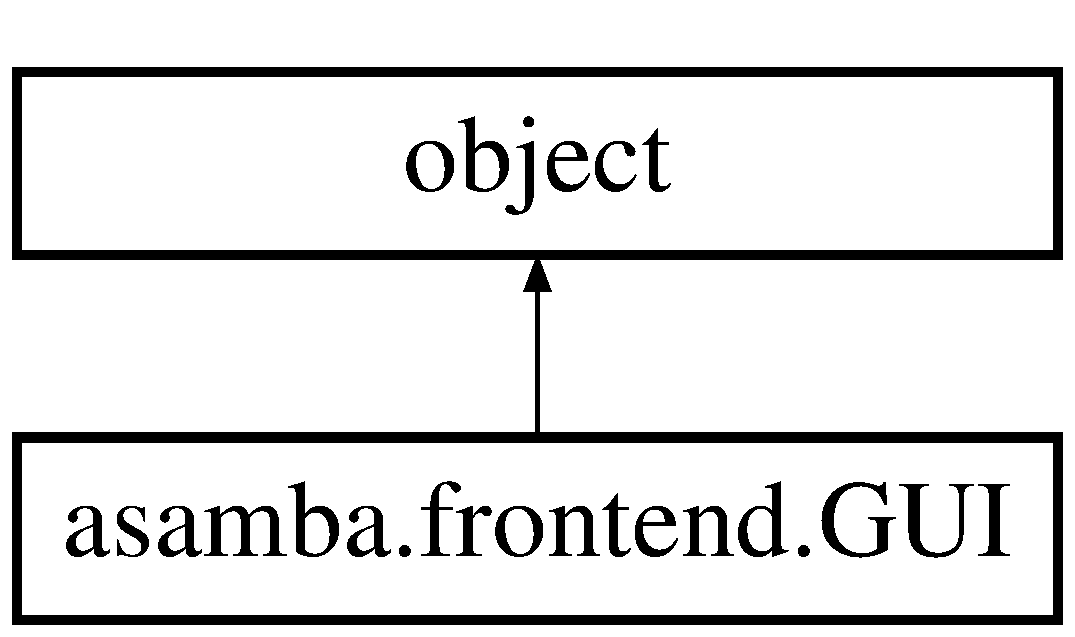
\includegraphics[height=2.000000cm]{classasamba_1_1frontend_1_1_g_u_i}
\end{center}
\end{figure}
\subsection*{Public Member Functions}
\begin{DoxyCompactItemize}
\item 
def \hyperlink{classasamba_1_1frontend_1_1_g_u_i_adff8117b4f723520f100119d38f9b567}{\+\_\+\+\_\+init\+\_\+\+\_\+} (self, root)
\item 
def \hyperlink{classasamba_1_1frontend_1_1_g_u_i_acaec11d5fbe0228d9da0e3ba10a4ea33}{Front\+Window} (self)
\item 
def \hyperlink{classasamba_1_1frontend_1_1_g_u_i_a4c88f62e31fe47af19c81215df643945}{connection\+\_\+choice} (self)
\item 
def \hyperlink{classasamba_1_1frontend_1_1_g_u_i_aacca71c626bd1753c1277e13b5ad8eec}{check\+\_\+connection} (self)
\item 
def \hyperlink{classasamba_1_1frontend_1_1_g_u_i_afb43aa6632c5aa17f9cf4a0270659a7f}{do\+\_\+connect} (self)
\item 
def \hyperlink{classasamba_1_1frontend_1_1_g_u_i_a905cc040d83a85cd64003f98b859a64a}{update\+\_\+connection\+\_\+state} (self)
\item 
def \hyperlink{classasamba_1_1frontend_1_1_g_u_i_aece59ad9eaff01043c324f9fa2175c98}{browse\+\_\+frequency\+\_\+file} (self)
\begin{DoxyCompactList}\small\item\em File Inputs. \end{DoxyCompactList}\item 
def \hyperlink{classasamba_1_1frontend_1_1_g_u_i_a515d6655fbf006441ec5ac9b96e5bd7c}{example\+\_\+input\+\_\+freq} (self)
\item 
def \hyperlink{classasamba_1_1frontend_1_1_g_u_i_addc94b5d78cdf85660cc6b2b61377252}{plot\+\_\+observed\+\_\+frequencies} (self)
\item 
def \hyperlink{classasamba_1_1frontend_1_1_g_u_i_a092f06f2cb8a31817b414a34f9dc52cf}{browse\+\_\+star\+\_\+file} (self)
\item 
def \hyperlink{classasamba_1_1frontend_1_1_g_u_i_a30a1139534dbd25b7635bd39c649a219}{example\+\_\+star\+\_\+inlist} (self)
\item 
def \hyperlink{classasamba_1_1frontend_1_1_g_u_i_ac0b39055d224594aca6190e6c0d7fe7e}{browse\+\_\+sampling\+\_\+file} (self)
\item 
def \hyperlink{classasamba_1_1frontend_1_1_g_u_i_a1a0a42d5c06ceb02b8a48dd7ff2f686e}{example\+\_\+sampling\+\_\+inlist} (self)
\item 
def \hyperlink{classasamba_1_1frontend_1_1_g_u_i_a118685a11c1f7602c17c22bc35419ef2}{call\+\_\+build\+\_\+learning\+\_\+set} (self)
\item 
def \hyperlink{classasamba_1_1frontend_1_1_g_u_i_a2f99fe1402d07c15d79897c8ec0ee4e0}{show\+\_\+samp\+\_\+results} (self)
\item 
def \hyperlink{classasamba_1_1frontend_1_1_g_u_i_a284b5146fbb37994b46e34ce48475f65}{split\+\_\+samp} (self)
\item 
def \hyperlink{classasamba_1_1frontend_1_1_g_u_i_a0e5bd5cd537353b15645f21196606524}{norm\+\_\+eq} (self)
\item 
def \hyperlink{classasamba_1_1frontend_1_1_g_u_i_a863beb8817b0f728771fcb3323afb043}{show\+\_\+norm\+\_\+eq\+\_\+result} (self)
\item 
def \hyperlink{classasamba_1_1frontend_1_1_g_u_i_a9b882f15d916eb942b202888fa29cf12}{update\+\_\+status\+\_\+bar} (self, message)
\end{DoxyCompactItemize}
\subsection*{Public Attributes}
\begin{DoxyCompactItemize}
\item 
\mbox{\Hypertarget{classasamba_1_1frontend_1_1_g_u_i_adfaa31df0ca0f60fb0edb1c8f51c1dab}\label{classasamba_1_1frontend_1_1_g_u_i_adfaa31df0ca0f60fb0edb1c8f51c1dab}} 
{\bfseries root}
\item 
\mbox{\Hypertarget{classasamba_1_1frontend_1_1_g_u_i_a6993546d0bc33283b1f23f78df4f5584}\label{classasamba_1_1frontend_1_1_g_u_i_a6993546d0bc33283b1f23f78df4f5584}} 
\hyperlink{classasamba_1_1frontend_1_1_g_u_i_a6993546d0bc33283b1f23f78df4f5584}{notebook}
\begin{DoxyCompactList}\small\item\em The root and the notebook. \end{DoxyCompactList}\item 
\mbox{\Hypertarget{classasamba_1_1frontend_1_1_g_u_i_ad1400ebbe0f0de8fdb2de1dfa4edec71}\label{classasamba_1_1frontend_1_1_g_u_i_ad1400ebbe0f0de8fdb2de1dfa4edec71}} 
{\bfseries dir\+\_\+data}
\item 
\mbox{\Hypertarget{classasamba_1_1frontend_1_1_g_u_i_a591824b1b84a6f16f79c9b5fa3d8ec4b}\label{classasamba_1_1frontend_1_1_g_u_i_a591824b1b84a6f16f79c9b5fa3d8ec4b}} 
{\bfseries dir\+\_\+bitmaps}
\item 
\mbox{\Hypertarget{classasamba_1_1frontend_1_1_g_u_i_a23ee533c711d07e9f8b698930fddb98a}\label{classasamba_1_1frontend_1_1_g_u_i_a23ee533c711d07e9f8b698930fddb98a}} 
\hyperlink{classasamba_1_1frontend_1_1_g_u_i_a23ee533c711d07e9f8b698930fddb98a}{tab\+\_\+seism}
\begin{DoxyCompactList}\small\item\em Tabs. \end{DoxyCompactList}\item 
\mbox{\Hypertarget{classasamba_1_1frontend_1_1_g_u_i_ad5f08477383ef1399461766f50823c96}\label{classasamba_1_1frontend_1_1_g_u_i_ad5f08477383ef1399461766f50823c96}} 
{\bfseries tab\+\_\+query}
\item 
\mbox{\Hypertarget{classasamba_1_1frontend_1_1_g_u_i_a4d7f4bcc774108ca48082a9975819331}\label{classasamba_1_1frontend_1_1_g_u_i_a4d7f4bcc774108ca48082a9975819331}} 
{\bfseries tab\+\_\+log}
\item 
\mbox{\Hypertarget{classasamba_1_1frontend_1_1_g_u_i_a53e06c13212fca9c491e8a5887925e09}\label{classasamba_1_1frontend_1_1_g_u_i_a53e06c13212fca9c491e8a5887925e09}} 
\hyperlink{classasamba_1_1frontend_1_1_g_u_i_a53e06c13212fca9c491e8a5887925e09}{frame\+\_\+conn}
\begin{DoxyCompactList}\small\item\em Mother \& Child Frames. \end{DoxyCompactList}\item 
\mbox{\Hypertarget{classasamba_1_1frontend_1_1_g_u_i_a9fa98e9c124d2d5d2ff58dcbafc01edf}\label{classasamba_1_1frontend_1_1_g_u_i_a9fa98e9c124d2d5d2ff58dcbafc01edf}} 
{\bfseries frame\+\_\+sample}
\item 
\mbox{\Hypertarget{classasamba_1_1frontend_1_1_g_u_i_a07fbff1b0ab5b17031b3b6acd7ac9b6c}\label{classasamba_1_1frontend_1_1_g_u_i_a07fbff1b0ab5b17031b3b6acd7ac9b6c}} 
{\bfseries frame\+\_\+\+M\+AP}
\item 
\mbox{\Hypertarget{classasamba_1_1frontend_1_1_g_u_i_aa42cba0eb02be7c755c74a35f1169fab}\label{classasamba_1_1frontend_1_1_g_u_i_aa42cba0eb02be7c755c74a35f1169fab}} 
{\bfseries frame\+\_\+input}
\item 
\mbox{\Hypertarget{classasamba_1_1frontend_1_1_g_u_i_a14034ec6f4f6ea938da2cf345686803d}\label{classasamba_1_1frontend_1_1_g_u_i_a14034ec6f4f6ea938da2cf345686803d}} 
{\bfseries frame\+\_\+interp}
\item 
\mbox{\Hypertarget{classasamba_1_1frontend_1_1_g_u_i_a7509cf35e7013100a020f570fafad33f}\label{classasamba_1_1frontend_1_1_g_u_i_a7509cf35e7013100a020f570fafad33f}} 
{\bfseries frame\+\_\+query}
\item 
\mbox{\Hypertarget{classasamba_1_1frontend_1_1_g_u_i_a338ff42655fa833bf03e50337551d154}\label{classasamba_1_1frontend_1_1_g_u_i_a338ff42655fa833bf03e50337551d154}} 
{\bfseries frame\+\_\+stat\+\_\+bar}
\item 
\mbox{\Hypertarget{classasamba_1_1frontend_1_1_g_u_i_a2e6e33452a8cee14657b7a31fe0f9fcc}\label{classasamba_1_1frontend_1_1_g_u_i_a2e6e33452a8cee14657b7a31fe0f9fcc}} 
{\bfseries connection}
\item 
\mbox{\Hypertarget{classasamba_1_1frontend_1_1_g_u_i_aca71293f8c32d7def189074bd89830d9}\label{classasamba_1_1frontend_1_1_g_u_i_aca71293f8c32d7def189074bd89830d9}} 
{\bfseries conn\+\_\+loc}
\item 
\mbox{\Hypertarget{classasamba_1_1frontend_1_1_g_u_i_aa6c77e3ecae07a73514859217d1e26ea}\label{classasamba_1_1frontend_1_1_g_u_i_aa6c77e3ecae07a73514859217d1e26ea}} 
{\bfseries conn\+\_\+loc\+\_\+str}
\item 
\mbox{\Hypertarget{classasamba_1_1frontend_1_1_g_u_i_a034978b933e1624c61b6c3ef558e9966}\label{classasamba_1_1frontend_1_1_g_u_i_a034978b933e1624c61b6c3ef558e9966}} 
{\bfseries conn\+\_\+ivs}
\item 
\mbox{\Hypertarget{classasamba_1_1frontend_1_1_g_u_i_a7e7330bb8b346fc85a3e8696842659a0}\label{classasamba_1_1frontend_1_1_g_u_i_a7e7330bb8b346fc85a3e8696842659a0}} 
{\bfseries conn\+\_\+ivs\+\_\+str}
\item 
\mbox{\Hypertarget{classasamba_1_1frontend_1_1_g_u_i_ae302af893ff2d00fa7f863c83c57d5ec}\label{classasamba_1_1frontend_1_1_g_u_i_ae302af893ff2d00fa7f863c83c57d5ec}} 
{\bfseries conn\+\_\+https}
\item 
\mbox{\Hypertarget{classasamba_1_1frontend_1_1_g_u_i_aa769c90f3ab4287a5111627c2ba7dea4}\label{classasamba_1_1frontend_1_1_g_u_i_aa769c90f3ab4287a5111627c2ba7dea4}} 
{\bfseries conn\+\_\+https\+\_\+str}
\item 
\mbox{\Hypertarget{classasamba_1_1frontend_1_1_g_u_i_a3b306cd67332dd5ea0583642c31b4fdd}\label{classasamba_1_1frontend_1_1_g_u_i_a3b306cd67332dd5ea0583642c31b4fdd}} 
{\bfseries dbname}
\item 
\mbox{\Hypertarget{classasamba_1_1frontend_1_1_g_u_i_ac22146dfa55dbe671ac1218fcb419035}\label{classasamba_1_1frontend_1_1_g_u_i_ac22146dfa55dbe671ac1218fcb419035}} 
{\bfseries conn\+\_\+status}
\item 
\mbox{\Hypertarget{classasamba_1_1frontend_1_1_g_u_i_acaa8c176334500a2440c93d8606b18af}\label{classasamba_1_1frontend_1_1_g_u_i_acaa8c176334500a2440c93d8606b18af}} 
{\bfseries conn\+\_\+lbl\+\_\+str}
\item 
\mbox{\Hypertarget{classasamba_1_1frontend_1_1_g_u_i_a611822ad3b47a5e10bd243a5ceec46dc}\label{classasamba_1_1frontend_1_1_g_u_i_a611822ad3b47a5e10bd243a5ceec46dc}} 
{\bfseries bitmap\+\_\+\+OK}
\item 
\mbox{\Hypertarget{classasamba_1_1frontend_1_1_g_u_i_a4db701e5b850e140443910ba250b794c}\label{classasamba_1_1frontend_1_1_g_u_i_a4db701e5b850e140443910ba250b794c}} 
{\bfseries bitmap\+\_\+\+N\+OK}
\item 
\mbox{\Hypertarget{classasamba_1_1frontend_1_1_g_u_i_af90df3728864c5e9740bd337d3eaf5b1}\label{classasamba_1_1frontend_1_1_g_u_i_af90df3728864c5e9740bd337d3eaf5b1}} 
{\bfseries input\+\_\+freq\+\_\+file}
\item 
\mbox{\Hypertarget{classasamba_1_1frontend_1_1_g_u_i_acae01bc46f8e0558bcd949523b5976e4}\label{classasamba_1_1frontend_1_1_g_u_i_acae01bc46f8e0558bcd949523b5976e4}} 
{\bfseries input\+\_\+freq\+\_\+done}
\item 
\mbox{\Hypertarget{classasamba_1_1frontend_1_1_g_u_i_a29832e3173ac16a017be629c215c2f1e}\label{classasamba_1_1frontend_1_1_g_u_i_a29832e3173ac16a017be629c215c2f1e}} 
{\bfseries star\+\_\+inlist}
\item 
\mbox{\Hypertarget{classasamba_1_1frontend_1_1_g_u_i_ad395df0b3f6ea80b9636bb27c4f092bc}\label{classasamba_1_1frontend_1_1_g_u_i_ad395df0b3f6ea80b9636bb27c4f092bc}} 
{\bfseries star\+\_\+inlist\+\_\+done}
\item 
\mbox{\Hypertarget{classasamba_1_1frontend_1_1_g_u_i_a7bdd62fb8ca976768f41546a6bc00edb}\label{classasamba_1_1frontend_1_1_g_u_i_a7bdd62fb8ca976768f41546a6bc00edb}} 
{\bfseries figure\+\_\+is\+\_\+shown}
\item 
\mbox{\Hypertarget{classasamba_1_1frontend_1_1_g_u_i_a92fe8ff60078991c372d4fdd2c331ed4}\label{classasamba_1_1frontend_1_1_g_u_i_a92fe8ff60078991c372d4fdd2c331ed4}} 
{\bfseries figure\+\_\+object}
\item 
\mbox{\Hypertarget{classasamba_1_1frontend_1_1_g_u_i_a12dae5c66955780ef9a3675a7f6a8346}\label{classasamba_1_1frontend_1_1_g_u_i_a12dae5c66955780ef9a3675a7f6a8346}} 
{\bfseries sampling\+\_\+inlist}
\item 
\mbox{\Hypertarget{classasamba_1_1frontend_1_1_g_u_i_a93f259d9ddc41bd5af93390f242ea6db}\label{classasamba_1_1frontend_1_1_g_u_i_a93f259d9ddc41bd5af93390f242ea6db}} 
{\bfseries sampling\+\_\+inlist\+\_\+done}
\item 
\mbox{\Hypertarget{classasamba_1_1frontend_1_1_g_u_i_ac9a577de855dc6c9404200d54d606796}\label{classasamba_1_1frontend_1_1_g_u_i_ac9a577de855dc6c9404200d54d606796}} 
{\bfseries build\+\_\+learning\+\_\+set\+\_\+done}
\item 
\mbox{\Hypertarget{classasamba_1_1frontend_1_1_g_u_i_a4f97c1f773aa04667c7f938fb5f65fcb}\label{classasamba_1_1frontend_1_1_g_u_i_a4f97c1f773aa04667c7f938fb5f65fcb}} 
{\bfseries norm\+\_\+eq\+\_\+done}
\item 
\mbox{\Hypertarget{classasamba_1_1frontend_1_1_g_u_i_a44b24df133e10e2cbbb9213f3777eb1b}\label{classasamba_1_1frontend_1_1_g_u_i_a44b24df133e10e2cbbb9213f3777eb1b}} 
{\bfseries status\+\_\+bar\+\_\+message}
\item 
\mbox{\Hypertarget{classasamba_1_1frontend_1_1_g_u_i_a94ee91aad33b7e700962853f629ddd0f}\label{classasamba_1_1frontend_1_1_g_u_i_a94ee91aad33b7e700962853f629ddd0f}} 
{\bfseries frame\+\_\+plot\+\_\+modes}
\item 
\mbox{\Hypertarget{classasamba_1_1frontend_1_1_g_u_i_aa0ed48e27bf3c1cf0f27e32c986f17a5}\label{classasamba_1_1frontend_1_1_g_u_i_aa0ed48e27bf3c1cf0f27e32c986f17a5}} 
\hyperlink{classasamba_1_1frontend_1_1_g_u_i_aa0ed48e27bf3c1cf0f27e32c986f17a5}{conn\+\_\+lbl}
\begin{DoxyCompactList}\small\item\em The connection frame. \end{DoxyCompactList}\item 
\mbox{\Hypertarget{classasamba_1_1frontend_1_1_g_u_i_ad013c21fae6ac840c1496a06c8df481f}\label{classasamba_1_1frontend_1_1_g_u_i_ad013c21fae6ac840c1496a06c8df481f}} 
\hyperlink{classasamba_1_1frontend_1_1_g_u_i_ad013c21fae6ac840c1496a06c8df481f}{but\+\_\+input\+\_\+freq}
\begin{DoxyCompactList}\small\item\em The Inputs Frame. \end{DoxyCompactList}\item 
\mbox{\Hypertarget{classasamba_1_1frontend_1_1_g_u_i_a60493d232fe6b161f24bf2dce1f40dd7}\label{classasamba_1_1frontend_1_1_g_u_i_a60493d232fe6b161f24bf2dce1f40dd7}} 
{\bfseries but\+\_\+ex\+\_\+freq}
\item 
\mbox{\Hypertarget{classasamba_1_1frontend_1_1_g_u_i_a40e7e816b472ee626cb370bd84428bd8}\label{classasamba_1_1frontend_1_1_g_u_i_a40e7e816b472ee626cb370bd84428bd8}} 
{\bfseries but\+\_\+input\+\_\+star}
\item 
\mbox{\Hypertarget{classasamba_1_1frontend_1_1_g_u_i_a48c3a6f9bb53cd556f3bfbfc282089b0}\label{classasamba_1_1frontend_1_1_g_u_i_a48c3a6f9bb53cd556f3bfbfc282089b0}} 
{\bfseries but\+\_\+input\+\_\+star\+\_\+ex}
\item 
\mbox{\Hypertarget{classasamba_1_1frontend_1_1_g_u_i_a5b907fc6ece0d97a2f81d3df8b5564f1}\label{classasamba_1_1frontend_1_1_g_u_i_a5b907fc6ece0d97a2f81d3df8b5564f1}} 
\hyperlink{classasamba_1_1frontend_1_1_g_u_i_a5b907fc6ece0d97a2f81d3df8b5564f1}{but\+\_\+samp\+\_\+input}
\begin{DoxyCompactList}\small\item\em The Sampling Frame. \end{DoxyCompactList}\item 
\mbox{\Hypertarget{classasamba_1_1frontend_1_1_g_u_i_a3b6543b0a1dcdd6bb0b1d586190cbe51}\label{classasamba_1_1frontend_1_1_g_u_i_a3b6543b0a1dcdd6bb0b1d586190cbe51}} 
{\bfseries but\+\_\+samp\+\_\+ex}
\item 
\mbox{\Hypertarget{classasamba_1_1frontend_1_1_g_u_i_abe6b8bb625709c304e7025d2f5fa627f}\label{classasamba_1_1frontend_1_1_g_u_i_abe6b8bb625709c304e7025d2f5fa627f}} 
{\bfseries but\+\_\+samp\+\_\+exec}
\item 
\mbox{\Hypertarget{classasamba_1_1frontend_1_1_g_u_i_a82904f7dbb17faed844632791969347f}\label{classasamba_1_1frontend_1_1_g_u_i_a82904f7dbb17faed844632791969347f}} 
{\bfseries but\+\_\+samp\+\_\+res}
\item 
\mbox{\Hypertarget{classasamba_1_1frontend_1_1_g_u_i_a290e3061b55eb81930101c4c55b499ae}\label{classasamba_1_1frontend_1_1_g_u_i_a290e3061b55eb81930101c4c55b499ae}} 
{\bfseries but\+\_\+samp\+\_\+slit}
\item 
\mbox{\Hypertarget{classasamba_1_1frontend_1_1_g_u_i_a0c2c425061ce1583c5311f029825acee}\label{classasamba_1_1frontend_1_1_g_u_i_a0c2c425061ce1583c5311f029825acee}} 
\hyperlink{classasamba_1_1frontend_1_1_g_u_i_a0c2c425061ce1583c5311f029825acee}{but\+\_\+norm\+\_\+eq}
\begin{DoxyCompactList}\small\item\em The Maximum a Posteriori Frame. \end{DoxyCompactList}\item 
\mbox{\Hypertarget{classasamba_1_1frontend_1_1_g_u_i_aee52575a258b715039867fd545b7b2ec}\label{classasamba_1_1frontend_1_1_g_u_i_aee52575a258b715039867fd545b7b2ec}} 
{\bfseries but\+\_\+norm\+\_\+eq\+\_\+res}
\item 
\mbox{\Hypertarget{classasamba_1_1frontend_1_1_g_u_i_a17dc5798170d2360729649e580634ee2}\label{classasamba_1_1frontend_1_1_g_u_i_a17dc5798170d2360729649e580634ee2}} 
{\bfseries but\+\_\+\+M\+AP}
\item 
\mbox{\Hypertarget{classasamba_1_1frontend_1_1_g_u_i_a7bbbdcf42f8093b1d870f19b7b05132b}\label{classasamba_1_1frontend_1_1_g_u_i_a7bbbdcf42f8093b1d870f19b7b05132b}} 
{\bfseries but\+\_\+\+M\+A\+P\+\_\+ex}
\item 
\mbox{\Hypertarget{classasamba_1_1frontend_1_1_g_u_i_a0b9c0994d8efbe779b1f57360f869b50}\label{classasamba_1_1frontend_1_1_g_u_i_a0b9c0994d8efbe779b1f57360f869b50}} 
{\bfseries but\+\_\+\+M\+A\+P\+\_\+exec}
\item 
\mbox{\Hypertarget{classasamba_1_1frontend_1_1_g_u_i_adc6412655d7034c60da54364e0228b73}\label{classasamba_1_1frontend_1_1_g_u_i_adc6412655d7034c60da54364e0228b73}} 
\hyperlink{classasamba_1_1frontend_1_1_g_u_i_adc6412655d7034c60da54364e0228b73}{but\+\_\+interp}
\begin{DoxyCompactList}\small\item\em The Interpolation Frame. \end{DoxyCompactList}\item 
\mbox{\Hypertarget{classasamba_1_1frontend_1_1_g_u_i_a2bb9f4e073b2187955cccad7898eccb7}\label{classasamba_1_1frontend_1_1_g_u_i_a2bb9f4e073b2187955cccad7898eccb7}} 
{\bfseries but\+\_\+interp\+\_\+ex}
\item 
\mbox{\Hypertarget{classasamba_1_1frontend_1_1_g_u_i_a8433ecadef42cf5f34172b222f2015f3}\label{classasamba_1_1frontend_1_1_g_u_i_a8433ecadef42cf5f34172b222f2015f3}} 
{\bfseries but\+\_\+interp\+\_\+exec}
\item 
\mbox{\Hypertarget{classasamba_1_1frontend_1_1_g_u_i_addea3bc3e768466ce68e55f4c1bcb5ea}\label{classasamba_1_1frontend_1_1_g_u_i_addea3bc3e768466ce68e55f4c1bcb5ea}} 
\hyperlink{classasamba_1_1frontend_1_1_g_u_i_addea3bc3e768466ce68e55f4c1bcb5ea}{but\+\_\+query}
\begin{DoxyCompactList}\small\item\em The Query Frame. \end{DoxyCompactList}\item 
\mbox{\Hypertarget{classasamba_1_1frontend_1_1_g_u_i_ae483448f532c86136af6c332c33528b8}\label{classasamba_1_1frontend_1_1_g_u_i_ae483448f532c86136af6c332c33528b8}} 
{\bfseries but\+\_\+query\+\_\+ex}
\item 
\mbox{\Hypertarget{classasamba_1_1frontend_1_1_g_u_i_aeed8a8ab709d60ac0d5d9e1180be5aea}\label{classasamba_1_1frontend_1_1_g_u_i_aeed8a8ab709d60ac0d5d9e1180be5aea}} 
{\bfseries but\+\_\+query\+\_\+exec}
\item 
\mbox{\Hypertarget{classasamba_1_1frontend_1_1_g_u_i_a4d992d23ea956c881ee49406c5bbac6b}\label{classasamba_1_1frontend_1_1_g_u_i_a4d992d23ea956c881ee49406c5bbac6b}} 
{\bfseries save\+\_\+query}
\item 
\hyperlink{classasamba_1_1frontend_1_1_g_u_i_a05a2765e23aaed2a4380f7089f387dbd}{status\+\_\+bar}
\begin{DoxyCompactList}\small\item\em Display observed data. \end{DoxyCompactList}\end{DoxyCompactItemize}


\subsection{Detailed Description}


Definition at line 56 of file frontend.\+py.



\subsection{Constructor \& Destructor Documentation}
\mbox{\Hypertarget{classasamba_1_1frontend_1_1_g_u_i_adff8117b4f723520f100119d38f9b567}\label{classasamba_1_1frontend_1_1_g_u_i_adff8117b4f723520f100119d38f9b567}} 
\index{asamba\+::frontend\+::\+G\+UI@{asamba\+::frontend\+::\+G\+UI}!\+\_\+\+\_\+init\+\_\+\+\_\+@{\+\_\+\+\_\+init\+\_\+\+\_\+}}
\index{\+\_\+\+\_\+init\+\_\+\+\_\+@{\+\_\+\+\_\+init\+\_\+\+\_\+}!asamba\+::frontend\+::\+G\+UI@{asamba\+::frontend\+::\+G\+UI}}
\subsubsection{\texorpdfstring{\+\_\+\+\_\+init\+\_\+\+\_\+()}{\_\_init\_\_()}}
{\footnotesize\ttfamily def asamba.\+frontend.\+G\+U\+I.\+\_\+\+\_\+init\+\_\+\+\_\+ (\begin{DoxyParamCaption}\item[{}]{self,  }\item[{}]{root }\end{DoxyParamCaption})}

\begin{DoxyVerb}Get an instance of the frontend GUI.

@param root: An instance of the tk.Tk() object
@type root: object
\end{DoxyVerb}
 

Definition at line 58 of file frontend.\+py.



\subsection{Member Function Documentation}
\mbox{\Hypertarget{classasamba_1_1frontend_1_1_g_u_i_aece59ad9eaff01043c324f9fa2175c98}\label{classasamba_1_1frontend_1_1_g_u_i_aece59ad9eaff01043c324f9fa2175c98}} 
\index{asamba\+::frontend\+::\+G\+UI@{asamba\+::frontend\+::\+G\+UI}!browse\+\_\+frequency\+\_\+file@{browse\+\_\+frequency\+\_\+file}}
\index{browse\+\_\+frequency\+\_\+file@{browse\+\_\+frequency\+\_\+file}!asamba\+::frontend\+::\+G\+UI@{asamba\+::frontend\+::\+G\+UI}}
\subsubsection{\texorpdfstring{browse\+\_\+frequency\+\_\+file()}{browse\_frequency\_file()}}
{\footnotesize\ttfamily def asamba.\+frontend.\+G\+U\+I.\+browse\+\_\+frequency\+\_\+file (\begin{DoxyParamCaption}\item[{}]{self }\end{DoxyParamCaption})}



File Inputs. 

\begin{DoxyVerb}Browse the local disk for an ASCII file \end{DoxyVerb}
 

Definition at line 370 of file frontend.\+py.

\mbox{\Hypertarget{classasamba_1_1frontend_1_1_g_u_i_ac0b39055d224594aca6190e6c0d7fe7e}\label{classasamba_1_1frontend_1_1_g_u_i_ac0b39055d224594aca6190e6c0d7fe7e}} 
\index{asamba\+::frontend\+::\+G\+UI@{asamba\+::frontend\+::\+G\+UI}!browse\+\_\+sampling\+\_\+file@{browse\+\_\+sampling\+\_\+file}}
\index{browse\+\_\+sampling\+\_\+file@{browse\+\_\+sampling\+\_\+file}!asamba\+::frontend\+::\+G\+UI@{asamba\+::frontend\+::\+G\+UI}}
\subsubsection{\texorpdfstring{browse\+\_\+sampling\+\_\+file()}{browse\_sampling\_file()}}
{\footnotesize\ttfamily def asamba.\+frontend.\+G\+U\+I.\+browse\+\_\+sampling\+\_\+file (\begin{DoxyParamCaption}\item[{}]{self }\end{DoxyParamCaption})}

\begin{DoxyVerb}Browse and locate the user-specified sampling inlist file \end{DoxyVerb}
 

Definition at line 486 of file frontend.\+py.

\mbox{\Hypertarget{classasamba_1_1frontend_1_1_g_u_i_a092f06f2cb8a31817b414a34f9dc52cf}\label{classasamba_1_1frontend_1_1_g_u_i_a092f06f2cb8a31817b414a34f9dc52cf}} 
\index{asamba\+::frontend\+::\+G\+UI@{asamba\+::frontend\+::\+G\+UI}!browse\+\_\+star\+\_\+file@{browse\+\_\+star\+\_\+file}}
\index{browse\+\_\+star\+\_\+file@{browse\+\_\+star\+\_\+file}!asamba\+::frontend\+::\+G\+UI@{asamba\+::frontend\+::\+G\+UI}}
\subsubsection{\texorpdfstring{browse\+\_\+star\+\_\+file()}{browse\_star\_file()}}
{\footnotesize\ttfamily def asamba.\+frontend.\+G\+U\+I.\+browse\+\_\+star\+\_\+file (\begin{DoxyParamCaption}\item[{}]{self }\end{DoxyParamCaption})}

\begin{DoxyVerb}Browse and locate the user-specified star inlist file \end{DoxyVerb}
 

Definition at line 460 of file frontend.\+py.

\mbox{\Hypertarget{classasamba_1_1frontend_1_1_g_u_i_a118685a11c1f7602c17c22bc35419ef2}\label{classasamba_1_1frontend_1_1_g_u_i_a118685a11c1f7602c17c22bc35419ef2}} 
\index{asamba\+::frontend\+::\+G\+UI@{asamba\+::frontend\+::\+G\+UI}!call\+\_\+build\+\_\+learning\+\_\+set@{call\+\_\+build\+\_\+learning\+\_\+set}}
\index{call\+\_\+build\+\_\+learning\+\_\+set@{call\+\_\+build\+\_\+learning\+\_\+set}!asamba\+::frontend\+::\+G\+UI@{asamba\+::frontend\+::\+G\+UI}}
\subsubsection{\texorpdfstring{call\+\_\+build\+\_\+learning\+\_\+set()}{call\_build\_learning\_set()}}
{\footnotesize\ttfamily def asamba.\+frontend.\+G\+U\+I.\+call\+\_\+build\+\_\+learning\+\_\+set (\begin{DoxyParamCaption}\item[{}]{self }\end{DoxyParamCaption})}

\begin{DoxyVerb}A wrapper to call sampler.build_learning_set through the backend \end{DoxyVerb}
 

Definition at line 512 of file frontend.\+py.

\mbox{\Hypertarget{classasamba_1_1frontend_1_1_g_u_i_aacca71c626bd1753c1277e13b5ad8eec}\label{classasamba_1_1frontend_1_1_g_u_i_aacca71c626bd1753c1277e13b5ad8eec}} 
\index{asamba\+::frontend\+::\+G\+UI@{asamba\+::frontend\+::\+G\+UI}!check\+\_\+connection@{check\+\_\+connection}}
\index{check\+\_\+connection@{check\+\_\+connection}!asamba\+::frontend\+::\+G\+UI@{asamba\+::frontend\+::\+G\+UI}}
\subsubsection{\texorpdfstring{check\+\_\+connection()}{check\_connection()}}
{\footnotesize\ttfamily def asamba.\+frontend.\+G\+U\+I.\+check\+\_\+connection (\begin{DoxyParamCaption}\item[{}]{self }\end{DoxyParamCaption})}

\begin{DoxyVerb}Try connecting to the database based on the user's choice \end{DoxyVerb}
 

Definition at line 335 of file frontend.\+py.

\mbox{\Hypertarget{classasamba_1_1frontend_1_1_g_u_i_a4c88f62e31fe47af19c81215df643945}\label{classasamba_1_1frontend_1_1_g_u_i_a4c88f62e31fe47af19c81215df643945}} 
\index{asamba\+::frontend\+::\+G\+UI@{asamba\+::frontend\+::\+G\+UI}!connection\+\_\+choice@{connection\+\_\+choice}}
\index{connection\+\_\+choice@{connection\+\_\+choice}!asamba\+::frontend\+::\+G\+UI@{asamba\+::frontend\+::\+G\+UI}}
\subsubsection{\texorpdfstring{connection\+\_\+choice()}{connection\_choice()}}
{\footnotesize\ttfamily def asamba.\+frontend.\+G\+U\+I.\+connection\+\_\+choice (\begin{DoxyParamCaption}\item[{}]{self }\end{DoxyParamCaption})}

\begin{DoxyVerb}Receive the 3 possible connection choices in int format \end{DoxyVerb}
 

Definition at line 326 of file frontend.\+py.

\mbox{\Hypertarget{classasamba_1_1frontend_1_1_g_u_i_afb43aa6632c5aa17f9cf4a0270659a7f}\label{classasamba_1_1frontend_1_1_g_u_i_afb43aa6632c5aa17f9cf4a0270659a7f}} 
\index{asamba\+::frontend\+::\+G\+UI@{asamba\+::frontend\+::\+G\+UI}!do\+\_\+connect@{do\+\_\+connect}}
\index{do\+\_\+connect@{do\+\_\+connect}!asamba\+::frontend\+::\+G\+UI@{asamba\+::frontend\+::\+G\+UI}}
\subsubsection{\texorpdfstring{do\+\_\+connect()}{do\_connect()}}
{\footnotesize\ttfamily def asamba.\+frontend.\+G\+U\+I.\+do\+\_\+connect (\begin{DoxyParamCaption}\item[{}]{self }\end{DoxyParamCaption})}

\begin{DoxyVerb}The backend will connect based on the user's connecton choice \end{DoxyVerb}
 

Definition at line 348 of file frontend.\+py.

\mbox{\Hypertarget{classasamba_1_1frontend_1_1_g_u_i_a515d6655fbf006441ec5ac9b96e5bd7c}\label{classasamba_1_1frontend_1_1_g_u_i_a515d6655fbf006441ec5ac9b96e5bd7c}} 
\index{asamba\+::frontend\+::\+G\+UI@{asamba\+::frontend\+::\+G\+UI}!example\+\_\+input\+\_\+freq@{example\+\_\+input\+\_\+freq}}
\index{example\+\_\+input\+\_\+freq@{example\+\_\+input\+\_\+freq}!asamba\+::frontend\+::\+G\+UI@{asamba\+::frontend\+::\+G\+UI}}
\subsubsection{\texorpdfstring{example\+\_\+input\+\_\+freq()}{example\_input\_freq()}}
{\footnotesize\ttfamily def asamba.\+frontend.\+G\+U\+I.\+example\+\_\+input\+\_\+freq (\begin{DoxyParamCaption}\item[{}]{self }\end{DoxyParamCaption})}

\begin{DoxyVerb}Show a static window with an example of how the input frequency file is structured \end{DoxyVerb}
 

Definition at line 386 of file frontend.\+py.

\mbox{\Hypertarget{classasamba_1_1frontend_1_1_g_u_i_a1a0a42d5c06ceb02b8a48dd7ff2f686e}\label{classasamba_1_1frontend_1_1_g_u_i_a1a0a42d5c06ceb02b8a48dd7ff2f686e}} 
\index{asamba\+::frontend\+::\+G\+UI@{asamba\+::frontend\+::\+G\+UI}!example\+\_\+sampling\+\_\+inlist@{example\+\_\+sampling\+\_\+inlist}}
\index{example\+\_\+sampling\+\_\+inlist@{example\+\_\+sampling\+\_\+inlist}!asamba\+::frontend\+::\+G\+UI@{asamba\+::frontend\+::\+G\+UI}}
\subsubsection{\texorpdfstring{example\+\_\+sampling\+\_\+inlist()}{example\_sampling\_inlist()}}
{\footnotesize\ttfamily def asamba.\+frontend.\+G\+U\+I.\+example\+\_\+sampling\+\_\+inlist (\begin{DoxyParamCaption}\item[{}]{self }\end{DoxyParamCaption})}

\begin{DoxyVerb}Show a static window with an example of how the sampling inlist file is structured \end{DoxyVerb}
 

Definition at line 501 of file frontend.\+py.

\mbox{\Hypertarget{classasamba_1_1frontend_1_1_g_u_i_a30a1139534dbd25b7635bd39c649a219}\label{classasamba_1_1frontend_1_1_g_u_i_a30a1139534dbd25b7635bd39c649a219}} 
\index{asamba\+::frontend\+::\+G\+UI@{asamba\+::frontend\+::\+G\+UI}!example\+\_\+star\+\_\+inlist@{example\+\_\+star\+\_\+inlist}}
\index{example\+\_\+star\+\_\+inlist@{example\+\_\+star\+\_\+inlist}!asamba\+::frontend\+::\+G\+UI@{asamba\+::frontend\+::\+G\+UI}}
\subsubsection{\texorpdfstring{example\+\_\+star\+\_\+inlist()}{example\_star\_inlist()}}
{\footnotesize\ttfamily def asamba.\+frontend.\+G\+U\+I.\+example\+\_\+star\+\_\+inlist (\begin{DoxyParamCaption}\item[{}]{self }\end{DoxyParamCaption})}

\begin{DoxyVerb}Show a static window with an example of how the star inlist file is structured \end{DoxyVerb}
 

Definition at line 475 of file frontend.\+py.

\mbox{\Hypertarget{classasamba_1_1frontend_1_1_g_u_i_acaec11d5fbe0228d9da0e3ba10a4ea33}\label{classasamba_1_1frontend_1_1_g_u_i_acaec11d5fbe0228d9da0e3ba10a4ea33}} 
\index{asamba\+::frontend\+::\+G\+UI@{asamba\+::frontend\+::\+G\+UI}!Front\+Window@{Front\+Window}}
\index{Front\+Window@{Front\+Window}!asamba\+::frontend\+::\+G\+UI@{asamba\+::frontend\+::\+G\+UI}}
\subsubsection{\texorpdfstring{Front\+Window()}{FrontWindow()}}
{\footnotesize\ttfamily def asamba.\+frontend.\+G\+U\+I.\+Front\+Window (\begin{DoxyParamCaption}\item[{}]{self }\end{DoxyParamCaption})}

\begin{DoxyVerb}The front GUI window \end{DoxyVerb}
 

Definition at line 133 of file frontend.\+py.

\mbox{\Hypertarget{classasamba_1_1frontend_1_1_g_u_i_a0e5bd5cd537353b15645f21196606524}\label{classasamba_1_1frontend_1_1_g_u_i_a0e5bd5cd537353b15645f21196606524}} 
\index{asamba\+::frontend\+::\+G\+UI@{asamba\+::frontend\+::\+G\+UI}!norm\+\_\+eq@{norm\+\_\+eq}}
\index{norm\+\_\+eq@{norm\+\_\+eq}!asamba\+::frontend\+::\+G\+UI@{asamba\+::frontend\+::\+G\+UI}}
\subsubsection{\texorpdfstring{norm\+\_\+eq()}{norm\_eq()}}
{\footnotesize\ttfamily def asamba.\+frontend.\+G\+U\+I.\+norm\+\_\+eq (\begin{DoxyParamCaption}\item[{}]{self }\end{DoxyParamCaption})}

\begin{DoxyVerb}a wrapper around bk.do_normal_eq \end{DoxyVerb}
 

Definition at line 565 of file frontend.\+py.

\mbox{\Hypertarget{classasamba_1_1frontend_1_1_g_u_i_addc94b5d78cdf85660cc6b2b61377252}\label{classasamba_1_1frontend_1_1_g_u_i_addc94b5d78cdf85660cc6b2b61377252}} 
\index{asamba\+::frontend\+::\+G\+UI@{asamba\+::frontend\+::\+G\+UI}!plot\+\_\+observed\+\_\+frequencies@{plot\+\_\+observed\+\_\+frequencies}}
\index{plot\+\_\+observed\+\_\+frequencies@{plot\+\_\+observed\+\_\+frequencies}!asamba\+::frontend\+::\+G\+UI@{asamba\+::frontend\+::\+G\+UI}}
\subsubsection{\texorpdfstring{plot\+\_\+observed\+\_\+frequencies()}{plot\_observed\_frequencies()}}
{\footnotesize\ttfamily def asamba.\+frontend.\+G\+U\+I.\+plot\+\_\+observed\+\_\+frequencies (\begin{DoxyParamCaption}\item[{}]{self }\end{DoxyParamCaption})}

\begin{DoxyVerb}If reading in put frequencies is successfull, the modes will be plotted, as a reward! \end{DoxyVerb}
 

Definition at line 397 of file frontend.\+py.

\mbox{\Hypertarget{classasamba_1_1frontend_1_1_g_u_i_a863beb8817b0f728771fcb3323afb043}\label{classasamba_1_1frontend_1_1_g_u_i_a863beb8817b0f728771fcb3323afb043}} 
\index{asamba\+::frontend\+::\+G\+UI@{asamba\+::frontend\+::\+G\+UI}!show\+\_\+norm\+\_\+eq\+\_\+result@{show\+\_\+norm\+\_\+eq\+\_\+result}}
\index{show\+\_\+norm\+\_\+eq\+\_\+result@{show\+\_\+norm\+\_\+eq\+\_\+result}!asamba\+::frontend\+::\+G\+UI@{asamba\+::frontend\+::\+G\+UI}}
\subsubsection{\texorpdfstring{show\+\_\+norm\+\_\+eq\+\_\+result()}{show\_norm\_eq\_result()}}
{\footnotesize\ttfamily def asamba.\+frontend.\+G\+U\+I.\+show\+\_\+norm\+\_\+eq\+\_\+result (\begin{DoxyParamCaption}\item[{}]{self }\end{DoxyParamCaption})}

\begin{DoxyVerb}Show the outcome of solving the normal equation \end{DoxyVerb}
 

Definition at line 582 of file frontend.\+py.

\mbox{\Hypertarget{classasamba_1_1frontend_1_1_g_u_i_a2f99fe1402d07c15d79897c8ec0ee4e0}\label{classasamba_1_1frontend_1_1_g_u_i_a2f99fe1402d07c15d79897c8ec0ee4e0}} 
\index{asamba\+::frontend\+::\+G\+UI@{asamba\+::frontend\+::\+G\+UI}!show\+\_\+samp\+\_\+results@{show\+\_\+samp\+\_\+results}}
\index{show\+\_\+samp\+\_\+results@{show\+\_\+samp\+\_\+results}!asamba\+::frontend\+::\+G\+UI@{asamba\+::frontend\+::\+G\+UI}}
\subsubsection{\texorpdfstring{show\+\_\+samp\+\_\+results()}{show\_samp\_results()}}
{\footnotesize\ttfamily def asamba.\+frontend.\+G\+U\+I.\+show\+\_\+samp\+\_\+results (\begin{DoxyParamCaption}\item[{}]{self }\end{DoxyParamCaption})}

\begin{DoxyVerb}Show the outcome of the sampling in a new pop up window \end{DoxyVerb}
 

Definition at line 545 of file frontend.\+py.

\mbox{\Hypertarget{classasamba_1_1frontend_1_1_g_u_i_a284b5146fbb37994b46e34ce48475f65}\label{classasamba_1_1frontend_1_1_g_u_i_a284b5146fbb37994b46e34ce48475f65}} 
\index{asamba\+::frontend\+::\+G\+UI@{asamba\+::frontend\+::\+G\+UI}!split\+\_\+samp@{split\+\_\+samp}}
\index{split\+\_\+samp@{split\+\_\+samp}!asamba\+::frontend\+::\+G\+UI@{asamba\+::frontend\+::\+G\+UI}}
\subsubsection{\texorpdfstring{split\+\_\+samp()}{split\_samp()}}
{\footnotesize\ttfamily def asamba.\+frontend.\+G\+U\+I.\+split\+\_\+samp (\begin{DoxyParamCaption}\item[{}]{self }\end{DoxyParamCaption})}

\begin{DoxyVerb}This is a wrapper around the bk.do_split_sample \end{DoxyVerb}
 

Definition at line 556 of file frontend.\+py.

\mbox{\Hypertarget{classasamba_1_1frontend_1_1_g_u_i_a905cc040d83a85cd64003f98b859a64a}\label{classasamba_1_1frontend_1_1_g_u_i_a905cc040d83a85cd64003f98b859a64a}} 
\index{asamba\+::frontend\+::\+G\+UI@{asamba\+::frontend\+::\+G\+UI}!update\+\_\+connection\+\_\+state@{update\+\_\+connection\+\_\+state}}
\index{update\+\_\+connection\+\_\+state@{update\+\_\+connection\+\_\+state}!asamba\+::frontend\+::\+G\+UI@{asamba\+::frontend\+::\+G\+UI}}
\subsubsection{\texorpdfstring{update\+\_\+connection\+\_\+state()}{update\_connection\_state()}}
{\footnotesize\ttfamily def asamba.\+frontend.\+G\+U\+I.\+update\+\_\+connection\+\_\+state (\begin{DoxyParamCaption}\item[{}]{self }\end{DoxyParamCaption})}

\begin{DoxyVerb}Update the label in the connection frame based on the connection test \end{DoxyVerb}
 

Definition at line 353 of file frontend.\+py.

\mbox{\Hypertarget{classasamba_1_1frontend_1_1_g_u_i_a9b882f15d916eb942b202888fa29cf12}\label{classasamba_1_1frontend_1_1_g_u_i_a9b882f15d916eb942b202888fa29cf12}} 
\index{asamba\+::frontend\+::\+G\+UI@{asamba\+::frontend\+::\+G\+UI}!update\+\_\+status\+\_\+bar@{update\+\_\+status\+\_\+bar}}
\index{update\+\_\+status\+\_\+bar@{update\+\_\+status\+\_\+bar}!asamba\+::frontend\+::\+G\+UI@{asamba\+::frontend\+::\+G\+UI}}
\subsubsection{\texorpdfstring{update\+\_\+status\+\_\+bar()}{update\_status\_bar()}}
{\footnotesize\ttfamily def asamba.\+frontend.\+G\+U\+I.\+update\+\_\+status\+\_\+bar (\begin{DoxyParamCaption}\item[{}]{self,  }\item[{}]{message }\end{DoxyParamCaption})}

\begin{DoxyVerb}Concurrently update the status printed on the StatusBar. Very handly method here! \end{DoxyVerb}
 

Definition at line 692 of file frontend.\+py.



\subsection{Member Data Documentation}
\mbox{\Hypertarget{classasamba_1_1frontend_1_1_g_u_i_a05a2765e23aaed2a4380f7089f387dbd}\label{classasamba_1_1frontend_1_1_g_u_i_a05a2765e23aaed2a4380f7089f387dbd}} 
\index{asamba\+::frontend\+::\+G\+UI@{asamba\+::frontend\+::\+G\+UI}!status\+\_\+bar@{status\+\_\+bar}}
\index{status\+\_\+bar@{status\+\_\+bar}!asamba\+::frontend\+::\+G\+UI@{asamba\+::frontend\+::\+G\+UI}}
\subsubsection{\texorpdfstring{status\+\_\+bar}{status\_bar}}
{\footnotesize\ttfamily asamba.\+frontend.\+G\+U\+I.\+status\+\_\+bar}



Display observed data. 

canv\+\_\+input\+\_\+freqs = tk.\+Canvas(inputs\+\_\+right, confine=False, cursor=\textquotesingle{}circle\textquotesingle{}, relief=\textquotesingle{}flat\textquotesingle{}) coord = 10, 50, 240, 240 arc = canv\+\_\+input\+\_\+freqs.\+create\+\_\+arc(coord, start=0, extent=150, fill=\char`\"{}blue\char`\"{}) canv\+\_\+input\+\_\+freqs.\+pack(side=\textquotesingle{}right\textquotesingle{}) Sampling, and online plotting frame

Canv\+\_\+plot\+\_\+1 = tk.\+Canvas(self.\+frame\+\_\+sample, confine=False) plot\+\_\+1\+\_\+file = tk.\+Photo\+Image(file==\textquotesingle{}Ehsan.\+J\+PG\textquotesingle{}) plot\+\_\+1 = Canv\+\_\+plot\+\_\+1.\+create\+\_\+image(500, 500, anchor=\textquotesingle{}center\textquotesingle{}, image=plot\+\_\+1\+\_\+file) Canv\+\_\+plot\+\_\+1.\+pack() Status Bar 

Definition at line 316 of file frontend.\+py.



The documentation for this class was generated from the following file\+:\begin{DoxyCompactItemize}
\item 
frontend.\+py\end{DoxyCompactItemize}

\hypertarget{classasamba_1_1frontend__orig_1_1_g_u_i}{}\section{asamba.\+frontend\+\_\+orig.\+G\+UI Class Reference}
\label{classasamba_1_1frontend__orig_1_1_g_u_i}\index{asamba.\+frontend\+\_\+orig.\+G\+UI@{asamba.\+frontend\+\_\+orig.\+G\+UI}}
Inheritance diagram for asamba.\+frontend\+\_\+orig.\+G\+UI\+:\begin{figure}[H]
\begin{center}
\leavevmode
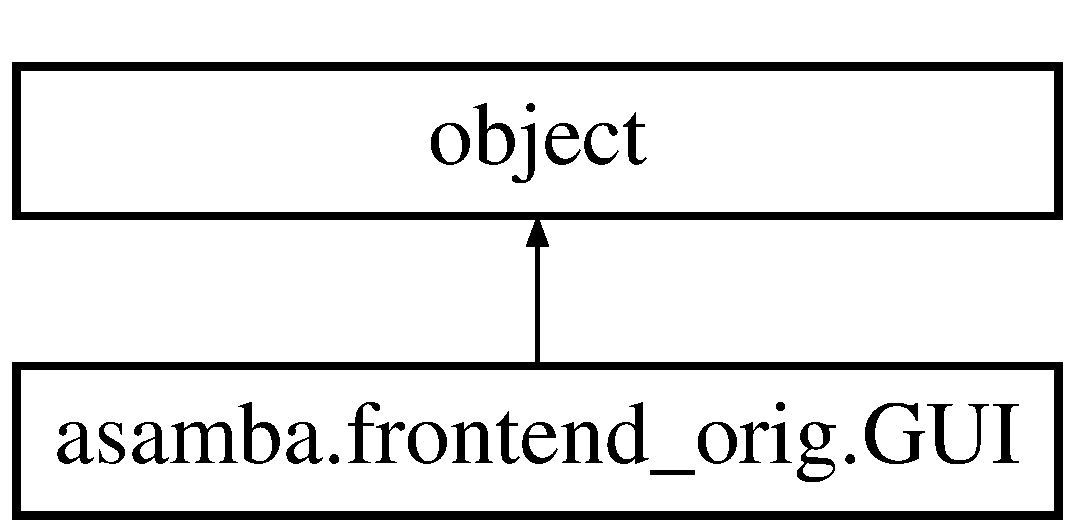
\includegraphics[height=2.000000cm]{classasamba_1_1frontend__orig_1_1_g_u_i}
\end{center}
\end{figure}
\subsection*{Public Member Functions}
\begin{DoxyCompactItemize}
\item 
\mbox{\Hypertarget{classasamba_1_1frontend__orig_1_1_g_u_i_a638a6ee5537927c1f13cdfacb5711168}\label{classasamba_1_1frontend__orig_1_1_g_u_i_a638a6ee5537927c1f13cdfacb5711168}} 
def {\bfseries \+\_\+\+\_\+init\+\_\+\+\_\+} (self, root)
\item 
def \hyperlink{classasamba_1_1frontend__orig_1_1_g_u_i_a0fd564268af273f977bc8065e26e110b}{Front\+Window} (self)
\item 
def \hyperlink{classasamba_1_1frontend__orig_1_1_g_u_i_af3fdec98d1b3657658a5f489b2246c34}{connection\+\_\+choice} (self)
\begin{DoxyCompactList}\small\item\em M E T H O D S. \end{DoxyCompactList}\item 
def \hyperlink{classasamba_1_1frontend__orig_1_1_g_u_i_ae71ecf0efcb575059e181ccd33f75178}{check\+\_\+connection} (self)
\item 
def \hyperlink{classasamba_1_1frontend__orig_1_1_g_u_i_a68a716eaa1fb6d82a7b004c77a5ab270}{do\+\_\+connect} (self)
\item 
def \hyperlink{classasamba_1_1frontend__orig_1_1_g_u_i_a4a594242291c4ab10089f279073ae8a7}{update\+\_\+connection\+\_\+state} (self)
\item 
def \hyperlink{classasamba_1_1frontend__orig_1_1_g_u_i_a5160be30a39afd49a2dd9ac4aba34d1d}{browse\+\_\+file} (self)
\begin{DoxyCompactList}\small\item\em File Inputs. \end{DoxyCompactList}\item 
def \hyperlink{classasamba_1_1frontend__orig_1_1_g_u_i_a6bb5f142abc9b56ccc0d7f9f7b3b99f1}{example\+\_\+input\+\_\+freq} (self)
\item 
def \hyperlink{classasamba_1_1frontend__orig_1_1_g_u_i_abb9e1670526f7bf28a6f2317e14546c0}{plot\+\_\+observed\+\_\+frequencies} (self)
\item 
def \hyperlink{classasamba_1_1frontend__orig_1_1_g_u_i_a5b038a5cef0239f96abd6accd44df396}{release\+\_\+obs\+\_\+log\+\_\+\+Teff} (self)
\begin{DoxyCompactList}\small\item\em Observatinal Inputs. \end{DoxyCompactList}\item 
def \hyperlink{classasamba_1_1frontend__orig_1_1_g_u_i_a23fecf5b0f52f4b0c420118e8572c435}{release\+\_\+obs\+\_\+log\+\_\+g} (self)
\item 
def \hyperlink{classasamba_1_1frontend__orig_1_1_g_u_i_a2115a025361cf5282c72baef51ec0004}{get\+\_\+observations} (self)
\item 
\mbox{\Hypertarget{classasamba_1_1frontend__orig_1_1_g_u_i_acd2f0daae2ef040bed9c496df0063cf6}\label{classasamba_1_1frontend__orig_1_1_g_u_i_acd2f0daae2ef040bed9c496df0063cf6}} 
def \hyperlink{classasamba_1_1frontend__orig_1_1_g_u_i_acd2f0daae2ef040bed9c496df0063cf6}{sampling\+\_\+setup} (self)
\begin{DoxyCompactList}\small\item\em Inputs through checkbuttons and radiobuttons. \end{DoxyCompactList}\item 
\mbox{\Hypertarget{classasamba_1_1frontend__orig_1_1_g_u_i_a0c1d59a9980bfd581ba746733429d620}\label{classasamba_1_1frontend__orig_1_1_g_u_i_a0c1d59a9980bfd581ba746733429d620}} 
def {\bfseries shuffling\+\_\+setup} (self)
\item 
def \hyperlink{classasamba_1_1frontend__orig_1_1_g_u_i_a630301b7e934776f232fcb4562974ae9}{update\+\_\+status\+\_\+bar} (self, message)
\begin{DoxyCompactList}\small\item\em Status Bar. \end{DoxyCompactList}\end{DoxyCompactItemize}
\subsection*{Public Attributes}
\begin{DoxyCompactItemize}
\item 
\mbox{\Hypertarget{classasamba_1_1frontend__orig_1_1_g_u_i_ab02ff442958e60c1104128219993990e}\label{classasamba_1_1frontend__orig_1_1_g_u_i_ab02ff442958e60c1104128219993990e}} 
{\bfseries root}
\item 
\mbox{\Hypertarget{classasamba_1_1frontend__orig_1_1_g_u_i_a0b733e9eedca186730369f6bc85cd07b}\label{classasamba_1_1frontend__orig_1_1_g_u_i_a0b733e9eedca186730369f6bc85cd07b}} 
{\bfseries dir\+\_\+data}
\item 
\mbox{\Hypertarget{classasamba_1_1frontend__orig_1_1_g_u_i_a16f3d14bb673617bee56685f37bb90a0}\label{classasamba_1_1frontend__orig_1_1_g_u_i_a16f3d14bb673617bee56685f37bb90a0}} 
{\bfseries dir\+\_\+bitmaps}
\item 
\mbox{\Hypertarget{classasamba_1_1frontend__orig_1_1_g_u_i_ab07d2cf890bce116c355b695ef3d69ee}\label{classasamba_1_1frontend__orig_1_1_g_u_i_ab07d2cf890bce116c355b695ef3d69ee}} 
\hyperlink{classasamba_1_1frontend__orig_1_1_g_u_i_ab07d2cf890bce116c355b695ef3d69ee}{frame\+\_\+conn}
\begin{DoxyCompactList}\small\item\em The mother frame and the children frames. \end{DoxyCompactList}\item 
\mbox{\Hypertarget{classasamba_1_1frontend__orig_1_1_g_u_i_aef02d079544f8eba516d753fa10f7252}\label{classasamba_1_1frontend__orig_1_1_g_u_i_aef02d079544f8eba516d753fa10f7252}} 
{\bfseries frame\+\_\+inputs}
\item 
\mbox{\Hypertarget{classasamba_1_1frontend__orig_1_1_g_u_i_a2215ed4456c55772765539da0ce4284f}\label{classasamba_1_1frontend__orig_1_1_g_u_i_a2215ed4456c55772765539da0ce4284f}} 
{\bfseries frame\+\_\+sample}
\item 
\mbox{\Hypertarget{classasamba_1_1frontend__orig_1_1_g_u_i_a2ffe91fef818d2e79621233b43e58973}\label{classasamba_1_1frontend__orig_1_1_g_u_i_a2ffe91fef818d2e79621233b43e58973}} 
{\bfseries frame\+\_\+\+M\+AP}
\item 
\mbox{\Hypertarget{classasamba_1_1frontend__orig_1_1_g_u_i_acd0b7f9e5c6ee7a96370ba1ac32b42cb}\label{classasamba_1_1frontend__orig_1_1_g_u_i_acd0b7f9e5c6ee7a96370ba1ac32b42cb}} 
{\bfseries frame\+\_\+stat\+\_\+bar}
\item 
\hyperlink{classasamba_1_1frontend__orig_1_1_g_u_i_a0c7f18b731c65f48e9cc27399e21363c}{inputs\+\_\+left}
\begin{DoxyCompactList}\small\item\em The inputs frame. \end{DoxyCompactList}\item 
\mbox{\Hypertarget{classasamba_1_1frontend__orig_1_1_g_u_i_aa6c810b3520d28a3584e67c70fb78271}\label{classasamba_1_1frontend__orig_1_1_g_u_i_aa6c810b3520d28a3584e67c70fb78271}} 
{\bfseries inputs\+\_\+right}
\item 
\mbox{\Hypertarget{classasamba_1_1frontend__orig_1_1_g_u_i_a6055bd3fe0b8485db6853a6dc9230c50}\label{classasamba_1_1frontend__orig_1_1_g_u_i_a6055bd3fe0b8485db6853a6dc9230c50}} 
{\bfseries connection}
\item 
\mbox{\Hypertarget{classasamba_1_1frontend__orig_1_1_g_u_i_ab7eddd0b03f5159cb7f6c8c7ef870e74}\label{classasamba_1_1frontend__orig_1_1_g_u_i_ab7eddd0b03f5159cb7f6c8c7ef870e74}} 
{\bfseries conn\+\_\+loc}
\item 
\mbox{\Hypertarget{classasamba_1_1frontend__orig_1_1_g_u_i_aae3f4b088a00e72a546148bfa8934be7}\label{classasamba_1_1frontend__orig_1_1_g_u_i_aae3f4b088a00e72a546148bfa8934be7}} 
{\bfseries conn\+\_\+loc\+\_\+str}
\item 
\mbox{\Hypertarget{classasamba_1_1frontend__orig_1_1_g_u_i_acdf60f8776cebfc6d04696feb7ae8d18}\label{classasamba_1_1frontend__orig_1_1_g_u_i_acdf60f8776cebfc6d04696feb7ae8d18}} 
{\bfseries conn\+\_\+ivs}
\item 
\mbox{\Hypertarget{classasamba_1_1frontend__orig_1_1_g_u_i_a77579d2cfd85ceacb8c3f4241635974b}\label{classasamba_1_1frontend__orig_1_1_g_u_i_a77579d2cfd85ceacb8c3f4241635974b}} 
{\bfseries conn\+\_\+ivs\+\_\+str}
\item 
\mbox{\Hypertarget{classasamba_1_1frontend__orig_1_1_g_u_i_a9db45d10c624479be0e5afe20479295f}\label{classasamba_1_1frontend__orig_1_1_g_u_i_a9db45d10c624479be0e5afe20479295f}} 
{\bfseries conn\+\_\+https}
\item 
\mbox{\Hypertarget{classasamba_1_1frontend__orig_1_1_g_u_i_a50ed9a673cd7873b024386cd8f5a3029}\label{classasamba_1_1frontend__orig_1_1_g_u_i_a50ed9a673cd7873b024386cd8f5a3029}} 
{\bfseries conn\+\_\+https\+\_\+str}
\item 
\mbox{\Hypertarget{classasamba_1_1frontend__orig_1_1_g_u_i_a84848ae7701a35e970a2d20f08ea5fc8}\label{classasamba_1_1frontend__orig_1_1_g_u_i_a84848ae7701a35e970a2d20f08ea5fc8}} 
{\bfseries dbname}
\item 
\mbox{\Hypertarget{classasamba_1_1frontend__orig_1_1_g_u_i_a0bdcc6318c315157f1292b7ce06effdd}\label{classasamba_1_1frontend__orig_1_1_g_u_i_a0bdcc6318c315157f1292b7ce06effdd}} 
{\bfseries conn\+\_\+status}
\item 
\mbox{\Hypertarget{classasamba_1_1frontend__orig_1_1_g_u_i_a400ad9f6b65f2537629a089835ea0f9f}\label{classasamba_1_1frontend__orig_1_1_g_u_i_a400ad9f6b65f2537629a089835ea0f9f}} 
{\bfseries conn\+\_\+lbl\+\_\+str}
\item 
\mbox{\Hypertarget{classasamba_1_1frontend__orig_1_1_g_u_i_af66c25399b7df5d82eef9694aca2cc4d}\label{classasamba_1_1frontend__orig_1_1_g_u_i_af66c25399b7df5d82eef9694aca2cc4d}} 
{\bfseries bitmap\+\_\+\+OK}
\item 
\mbox{\Hypertarget{classasamba_1_1frontend__orig_1_1_g_u_i_a0b311f182ac16067c0a60389601c2ec0}\label{classasamba_1_1frontend__orig_1_1_g_u_i_a0b311f182ac16067c0a60389601c2ec0}} 
{\bfseries bitmap\+\_\+\+N\+OK}
\item 
\mbox{\Hypertarget{classasamba_1_1frontend__orig_1_1_g_u_i_a1b58d97c43798befcf9e5040a9e81dd8}\label{classasamba_1_1frontend__orig_1_1_g_u_i_a1b58d97c43798befcf9e5040a9e81dd8}} 
{\bfseries input\+\_\+freq\+\_\+file}
\item 
\mbox{\Hypertarget{classasamba_1_1frontend__orig_1_1_g_u_i_a3d9f55f39d3d97cb6934d04603ae1a28}\label{classasamba_1_1frontend__orig_1_1_g_u_i_a3d9f55f39d3d97cb6934d04603ae1a28}} 
{\bfseries input\+\_\+freq\+\_\+done}
\item 
\mbox{\Hypertarget{classasamba_1_1frontend__orig_1_1_g_u_i_a0e30730af5ec63b823a9ceb5bf232a33}\label{classasamba_1_1frontend__orig_1_1_g_u_i_a0e30730af5ec63b823a9ceb5bf232a33}} 
{\bfseries use\+\_\+obs\+\_\+log\+\_\+\+Teff}
\item 
\mbox{\Hypertarget{classasamba_1_1frontend__orig_1_1_g_u_i_a342a7375a5f9b72d5b16be019c5e6f2f}\label{classasamba_1_1frontend__orig_1_1_g_u_i_a342a7375a5f9b72d5b16be019c5e6f2f}} 
{\bfseries obs\+\_\+log\+\_\+\+Teff}
\item 
\mbox{\Hypertarget{classasamba_1_1frontend__orig_1_1_g_u_i_a6a46561369e3e593ded888c48c650d4e}\label{classasamba_1_1frontend__orig_1_1_g_u_i_a6a46561369e3e593ded888c48c650d4e}} 
{\bfseries obs\+\_\+log\+\_\+\+Teff\+\_\+err}
\item 
\mbox{\Hypertarget{classasamba_1_1frontend__orig_1_1_g_u_i_ab2b662856c77f135a345ce19fd0f4815}\label{classasamba_1_1frontend__orig_1_1_g_u_i_ab2b662856c77f135a345ce19fd0f4815}} 
{\bfseries use\+\_\+obs\+\_\+log\+\_\+g}
\item 
\mbox{\Hypertarget{classasamba_1_1frontend__orig_1_1_g_u_i_ab0e7fb879ece2e7d8bfc52327c4a50ed}\label{classasamba_1_1frontend__orig_1_1_g_u_i_ab0e7fb879ece2e7d8bfc52327c4a50ed}} 
{\bfseries obs\+\_\+log\+\_\+g}
\item 
\mbox{\Hypertarget{classasamba_1_1frontend__orig_1_1_g_u_i_afa05b2e23d04a406ae312f5a605d3a60}\label{classasamba_1_1frontend__orig_1_1_g_u_i_afa05b2e23d04a406ae312f5a605d3a60}} 
{\bfseries obs\+\_\+log\+\_\+g\+\_\+err}
\item 
\mbox{\Hypertarget{classasamba_1_1frontend__orig_1_1_g_u_i_a3aff2f426976da0c2168350ba598d349}\label{classasamba_1_1frontend__orig_1_1_g_u_i_a3aff2f426976da0c2168350ba598d349}} 
{\bfseries which\+\_\+sampling\+\_\+function}
\item 
\mbox{\Hypertarget{classasamba_1_1frontend__orig_1_1_g_u_i_adc3189e05c49b045086f800edfbdd2c3}\label{classasamba_1_1frontend__orig_1_1_g_u_i_adc3189e05c49b045086f800edfbdd2c3}} 
{\bfseries sampling\+\_\+constrained}
\item 
\mbox{\Hypertarget{classasamba_1_1frontend__orig_1_1_g_u_i_aa0081c5aed1d4db293c2b2cf2d8181e0}\label{classasamba_1_1frontend__orig_1_1_g_u_i_aa0081c5aed1d4db293c2b2cf2d8181e0}} 
{\bfseries sampling\+\_\+randomly}
\item 
\mbox{\Hypertarget{classasamba_1_1frontend__orig_1_1_g_u_i_a4cb2c99d340526fde8668a723e8f80c1}\label{classasamba_1_1frontend__orig_1_1_g_u_i_a4cb2c99d340526fde8668a723e8f80c1}} 
{\bfseries sampling\+\_\+shuffle}
\item 
\mbox{\Hypertarget{classasamba_1_1frontend__orig_1_1_g_u_i_a5c5566251563f8a1047c3ea0dbdca00e}\label{classasamba_1_1frontend__orig_1_1_g_u_i_a5c5566251563f8a1047c3ea0dbdca00e}} 
{\bfseries status\+\_\+bar\+\_\+message}
\item 
\hyperlink{classasamba_1_1frontend__orig_1_1_g_u_i_a8ffe858f422b6affa1bc05765e05f360}{conn\+\_\+lbl}
\begin{DoxyCompactList}\small\item\em The connection frame. \end{DoxyCompactList}\item 
\mbox{\Hypertarget{classasamba_1_1frontend__orig_1_1_g_u_i_ad6f8fdbe540dbfef29c702860d6f58a0}\label{classasamba_1_1frontend__orig_1_1_g_u_i_ad6f8fdbe540dbfef29c702860d6f58a0}} 
{\bfseries but\+\_\+input\+\_\+freq}
\item 
\mbox{\Hypertarget{classasamba_1_1frontend__orig_1_1_g_u_i_a342dd1cbe401e79c9af53af7a1138ac3}\label{classasamba_1_1frontend__orig_1_1_g_u_i_a342dd1cbe401e79c9af53af7a1138ac3}} 
{\bfseries but\+\_\+ex\+\_\+freq}
\item 
\mbox{\Hypertarget{classasamba_1_1frontend__orig_1_1_g_u_i_a3d44da8ea42b14a41104b3e8073bbb3b}\label{classasamba_1_1frontend__orig_1_1_g_u_i_a3d44da8ea42b14a41104b3e8073bbb3b}} 
{\bfseries but\+\_\+input\+\_\+options}
\item 
\mbox{\Hypertarget{classasamba_1_1frontend__orig_1_1_g_u_i_ae8e9d8c8efc84c6304f2754c8c761bad}\label{classasamba_1_1frontend__orig_1_1_g_u_i_ae8e9d8c8efc84c6304f2754c8c761bad}} 
{\bfseries ckbx\+\_\+obs\+\_\+log\+\_\+\+Teff}
\item 
\mbox{\Hypertarget{classasamba_1_1frontend__orig_1_1_g_u_i_a0e78e7b94ce4e3b5d4ec3dacf31eadc5}\label{classasamba_1_1frontend__orig_1_1_g_u_i_a0e78e7b94ce4e3b5d4ec3dacf31eadc5}} 
{\bfseries enter\+\_\+log\+\_\+\+Teff}
\item 
\mbox{\Hypertarget{classasamba_1_1frontend__orig_1_1_g_u_i_a07cdf3c62b5a8b4f105e4780d6ac1b48}\label{classasamba_1_1frontend__orig_1_1_g_u_i_a07cdf3c62b5a8b4f105e4780d6ac1b48}} 
{\bfseries enter\+\_\+log\+\_\+\+Teff\+\_\+err}
\item 
\mbox{\Hypertarget{classasamba_1_1frontend__orig_1_1_g_u_i_a7fae7dc453da27ff35055a90dd3dd0a3}\label{classasamba_1_1frontend__orig_1_1_g_u_i_a7fae7dc453da27ff35055a90dd3dd0a3}} 
{\bfseries ckbx\+\_\+obs\+\_\+log\+\_\+g}
\item 
\mbox{\Hypertarget{classasamba_1_1frontend__orig_1_1_g_u_i_a84ef8a4f9716a5711c2909d0e8d96849}\label{classasamba_1_1frontend__orig_1_1_g_u_i_a84ef8a4f9716a5711c2909d0e8d96849}} 
{\bfseries enter\+\_\+log\+\_\+g}
\item 
\mbox{\Hypertarget{classasamba_1_1frontend__orig_1_1_g_u_i_a90efddcd0291cf8104d2b3fda8283e53}\label{classasamba_1_1frontend__orig_1_1_g_u_i_a90efddcd0291cf8104d2b3fda8283e53}} 
{\bfseries enter\+\_\+log\+\_\+g\+\_\+err}
\item 
\mbox{\Hypertarget{classasamba_1_1frontend__orig_1_1_g_u_i_ac80587243a92132f085069f5b28eaea7}\label{classasamba_1_1frontend__orig_1_1_g_u_i_ac80587243a92132f085069f5b28eaea7}} 
{\bfseries but\+\_\+obs}
\item 
\mbox{\Hypertarget{classasamba_1_1frontend__orig_1_1_g_u_i_a65ec52757fcf6b5536b4d118492fa289}\label{classasamba_1_1frontend__orig_1_1_g_u_i_a65ec52757fcf6b5536b4d118492fa289}} 
{\bfseries but\+\_\+ex\+\_\+options}
\item 
\mbox{\Hypertarget{classasamba_1_1frontend__orig_1_1_g_u_i_a182406307449b99c24581349d121efbd}\label{classasamba_1_1frontend__orig_1_1_g_u_i_a182406307449b99c24581349d121efbd}} 
{\bfseries rad\+\_\+but\+\_\+samp\+\_\+cnstr}
\item 
\mbox{\Hypertarget{classasamba_1_1frontend__orig_1_1_g_u_i_a475e4be23a060b2e8594f745f182d69b}\label{classasamba_1_1frontend__orig_1_1_g_u_i_a475e4be23a060b2e8594f745f182d69b}} 
{\bfseries rad\+\_\+but\+\_\+samp\+\_\+rand}
\item 
\mbox{\Hypertarget{classasamba_1_1frontend__orig_1_1_g_u_i_a8e40d620a0d6c1376a716a50b580c7f2}\label{classasamba_1_1frontend__orig_1_1_g_u_i_a8e40d620a0d6c1376a716a50b580c7f2}} 
{\bfseries ckbx\+\_\+sampling\+\_\+shuffle}
\item 
\hyperlink{classasamba_1_1frontend__orig_1_1_g_u_i_a740ec5fcacbc2e7b4fa0ea061b52d411}{status\+\_\+bar}
\begin{DoxyCompactList}\small\item\em Display observed data. \end{DoxyCompactList}\end{DoxyCompactItemize}


\subsection{Detailed Description}


Definition at line 39 of file frontend\+\_\+orig.\+py.



\subsection{Member Function Documentation}
\mbox{\Hypertarget{classasamba_1_1frontend__orig_1_1_g_u_i_a5160be30a39afd49a2dd9ac4aba34d1d}\label{classasamba_1_1frontend__orig_1_1_g_u_i_a5160be30a39afd49a2dd9ac4aba34d1d}} 
\index{asamba\+::frontend\+\_\+orig\+::\+G\+UI@{asamba\+::frontend\+\_\+orig\+::\+G\+UI}!browse\+\_\+file@{browse\+\_\+file}}
\index{browse\+\_\+file@{browse\+\_\+file}!asamba\+::frontend\+\_\+orig\+::\+G\+UI@{asamba\+::frontend\+\_\+orig\+::\+G\+UI}}
\subsubsection{\texorpdfstring{browse\+\_\+file()}{browse\_file()}}
{\footnotesize\ttfamily def asamba.\+frontend\+\_\+orig.\+G\+U\+I.\+browse\+\_\+file (\begin{DoxyParamCaption}\item[{}]{self }\end{DoxyParamCaption})}



File Inputs. 

\begin{DoxyVerb}Browse the local disk for an ASCII file \end{DoxyVerb}
 

Definition at line 349 of file frontend\+\_\+orig.\+py.

\mbox{\Hypertarget{classasamba_1_1frontend__orig_1_1_g_u_i_ae71ecf0efcb575059e181ccd33f75178}\label{classasamba_1_1frontend__orig_1_1_g_u_i_ae71ecf0efcb575059e181ccd33f75178}} 
\index{asamba\+::frontend\+\_\+orig\+::\+G\+UI@{asamba\+::frontend\+\_\+orig\+::\+G\+UI}!check\+\_\+connection@{check\+\_\+connection}}
\index{check\+\_\+connection@{check\+\_\+connection}!asamba\+::frontend\+\_\+orig\+::\+G\+UI@{asamba\+::frontend\+\_\+orig\+::\+G\+UI}}
\subsubsection{\texorpdfstring{check\+\_\+connection()}{check\_connection()}}
{\footnotesize\ttfamily def asamba.\+frontend\+\_\+orig.\+G\+U\+I.\+check\+\_\+connection (\begin{DoxyParamCaption}\item[{}]{self }\end{DoxyParamCaption})}

\begin{DoxyVerb}Try connecting to the database based on the user's choice \end{DoxyVerb}
 

Definition at line 315 of file frontend\+\_\+orig.\+py.

\mbox{\Hypertarget{classasamba_1_1frontend__orig_1_1_g_u_i_af3fdec98d1b3657658a5f489b2246c34}\label{classasamba_1_1frontend__orig_1_1_g_u_i_af3fdec98d1b3657658a5f489b2246c34}} 
\index{asamba\+::frontend\+\_\+orig\+::\+G\+UI@{asamba\+::frontend\+\_\+orig\+::\+G\+UI}!connection\+\_\+choice@{connection\+\_\+choice}}
\index{connection\+\_\+choice@{connection\+\_\+choice}!asamba\+::frontend\+\_\+orig\+::\+G\+UI@{asamba\+::frontend\+\_\+orig\+::\+G\+UI}}
\subsubsection{\texorpdfstring{connection\+\_\+choice()}{connection\_choice()}}
{\footnotesize\ttfamily def asamba.\+frontend\+\_\+orig.\+G\+U\+I.\+connection\+\_\+choice (\begin{DoxyParamCaption}\item[{}]{self }\end{DoxyParamCaption})}



M E T H O D S. 

Connection \begin{DoxyVerb}Receive the 3 possible connection choices in int format \end{DoxyVerb}
 

Definition at line 306 of file frontend\+\_\+orig.\+py.

\mbox{\Hypertarget{classasamba_1_1frontend__orig_1_1_g_u_i_a68a716eaa1fb6d82a7b004c77a5ab270}\label{classasamba_1_1frontend__orig_1_1_g_u_i_a68a716eaa1fb6d82a7b004c77a5ab270}} 
\index{asamba\+::frontend\+\_\+orig\+::\+G\+UI@{asamba\+::frontend\+\_\+orig\+::\+G\+UI}!do\+\_\+connect@{do\+\_\+connect}}
\index{do\+\_\+connect@{do\+\_\+connect}!asamba\+::frontend\+\_\+orig\+::\+G\+UI@{asamba\+::frontend\+\_\+orig\+::\+G\+UI}}
\subsubsection{\texorpdfstring{do\+\_\+connect()}{do\_connect()}}
{\footnotesize\ttfamily def asamba.\+frontend\+\_\+orig.\+G\+U\+I.\+do\+\_\+connect (\begin{DoxyParamCaption}\item[{}]{self }\end{DoxyParamCaption})}

\begin{DoxyVerb}The backend will connect based on the user's connecton choice \end{DoxyVerb}
 

Definition at line 328 of file frontend\+\_\+orig.\+py.

\mbox{\Hypertarget{classasamba_1_1frontend__orig_1_1_g_u_i_a6bb5f142abc9b56ccc0d7f9f7b3b99f1}\label{classasamba_1_1frontend__orig_1_1_g_u_i_a6bb5f142abc9b56ccc0d7f9f7b3b99f1}} 
\index{asamba\+::frontend\+\_\+orig\+::\+G\+UI@{asamba\+::frontend\+\_\+orig\+::\+G\+UI}!example\+\_\+input\+\_\+freq@{example\+\_\+input\+\_\+freq}}
\index{example\+\_\+input\+\_\+freq@{example\+\_\+input\+\_\+freq}!asamba\+::frontend\+\_\+orig\+::\+G\+UI@{asamba\+::frontend\+\_\+orig\+::\+G\+UI}}
\subsubsection{\texorpdfstring{example\+\_\+input\+\_\+freq()}{example\_input\_freq()}}
{\footnotesize\ttfamily def asamba.\+frontend\+\_\+orig.\+G\+U\+I.\+example\+\_\+input\+\_\+freq (\begin{DoxyParamCaption}\item[{}]{self }\end{DoxyParamCaption})}

\begin{DoxyVerb}Show a static window with an example of how the input frequency file is structured \end{DoxyVerb}
 

Definition at line 365 of file frontend\+\_\+orig.\+py.

\mbox{\Hypertarget{classasamba_1_1frontend__orig_1_1_g_u_i_a0fd564268af273f977bc8065e26e110b}\label{classasamba_1_1frontend__orig_1_1_g_u_i_a0fd564268af273f977bc8065e26e110b}} 
\index{asamba\+::frontend\+\_\+orig\+::\+G\+UI@{asamba\+::frontend\+\_\+orig\+::\+G\+UI}!Front\+Window@{Front\+Window}}
\index{Front\+Window@{Front\+Window}!asamba\+::frontend\+\_\+orig\+::\+G\+UI@{asamba\+::frontend\+\_\+orig\+::\+G\+UI}}
\subsubsection{\texorpdfstring{Front\+Window()}{FrontWindow()}}
{\footnotesize\ttfamily def asamba.\+frontend\+\_\+orig.\+G\+U\+I.\+Front\+Window (\begin{DoxyParamCaption}\item[{}]{self }\end{DoxyParamCaption})}

\begin{DoxyVerb}The front GUI window \end{DoxyVerb}
 

Definition at line 100 of file frontend\+\_\+orig.\+py.

\mbox{\Hypertarget{classasamba_1_1frontend__orig_1_1_g_u_i_a2115a025361cf5282c72baef51ec0004}\label{classasamba_1_1frontend__orig_1_1_g_u_i_a2115a025361cf5282c72baef51ec0004}} 
\index{asamba\+::frontend\+\_\+orig\+::\+G\+UI@{asamba\+::frontend\+\_\+orig\+::\+G\+UI}!get\+\_\+observations@{get\+\_\+observations}}
\index{get\+\_\+observations@{get\+\_\+observations}!asamba\+::frontend\+\_\+orig\+::\+G\+UI@{asamba\+::frontend\+\_\+orig\+::\+G\+UI}}
\subsubsection{\texorpdfstring{get\+\_\+observations()}{get\_observations()}}
{\footnotesize\ttfamily def asamba.\+frontend\+\_\+orig.\+G\+U\+I.\+get\+\_\+observations (\begin{DoxyParamCaption}\item[{}]{self }\end{DoxyParamCaption})}

\begin{DoxyVerb}Get all the observed values which are set in Entry boxes \end{DoxyVerb}
 

Definition at line 423 of file frontend\+\_\+orig.\+py.

\mbox{\Hypertarget{classasamba_1_1frontend__orig_1_1_g_u_i_abb9e1670526f7bf28a6f2317e14546c0}\label{classasamba_1_1frontend__orig_1_1_g_u_i_abb9e1670526f7bf28a6f2317e14546c0}} 
\index{asamba\+::frontend\+\_\+orig\+::\+G\+UI@{asamba\+::frontend\+\_\+orig\+::\+G\+UI}!plot\+\_\+observed\+\_\+frequencies@{plot\+\_\+observed\+\_\+frequencies}}
\index{plot\+\_\+observed\+\_\+frequencies@{plot\+\_\+observed\+\_\+frequencies}!asamba\+::frontend\+\_\+orig\+::\+G\+UI@{asamba\+::frontend\+\_\+orig\+::\+G\+UI}}
\subsubsection{\texorpdfstring{plot\+\_\+observed\+\_\+frequencies()}{plot\_observed\_frequencies()}}
{\footnotesize\ttfamily def asamba.\+frontend\+\_\+orig.\+G\+U\+I.\+plot\+\_\+observed\+\_\+frequencies (\begin{DoxyParamCaption}\item[{}]{self }\end{DoxyParamCaption})}

\begin{DoxyVerb}If reading in put frequencies is successfull, the modes will be plotted, as a reward! \end{DoxyVerb}
 

Definition at line 377 of file frontend\+\_\+orig.\+py.

\mbox{\Hypertarget{classasamba_1_1frontend__orig_1_1_g_u_i_a23fecf5b0f52f4b0c420118e8572c435}\label{classasamba_1_1frontend__orig_1_1_g_u_i_a23fecf5b0f52f4b0c420118e8572c435}} 
\index{asamba\+::frontend\+\_\+orig\+::\+G\+UI@{asamba\+::frontend\+\_\+orig\+::\+G\+UI}!release\+\_\+obs\+\_\+log\+\_\+g@{release\+\_\+obs\+\_\+log\+\_\+g}}
\index{release\+\_\+obs\+\_\+log\+\_\+g@{release\+\_\+obs\+\_\+log\+\_\+g}!asamba\+::frontend\+\_\+orig\+::\+G\+UI@{asamba\+::frontend\+\_\+orig\+::\+G\+UI}}
\subsubsection{\texorpdfstring{release\+\_\+obs\+\_\+log\+\_\+g()}{release\_obs\_log\_g()}}
{\footnotesize\ttfamily def asamba.\+frontend\+\_\+orig.\+G\+U\+I.\+release\+\_\+obs\+\_\+log\+\_\+g (\begin{DoxyParamCaption}\item[{}]{self }\end{DoxyParamCaption})}

\begin{DoxyVerb}Release the log_g two entry boxes \end{DoxyVerb}
 

Definition at line 415 of file frontend\+\_\+orig.\+py.

\mbox{\Hypertarget{classasamba_1_1frontend__orig_1_1_g_u_i_a5b038a5cef0239f96abd6accd44df396}\label{classasamba_1_1frontend__orig_1_1_g_u_i_a5b038a5cef0239f96abd6accd44df396}} 
\index{asamba\+::frontend\+\_\+orig\+::\+G\+UI@{asamba\+::frontend\+\_\+orig\+::\+G\+UI}!release\+\_\+obs\+\_\+log\+\_\+\+Teff@{release\+\_\+obs\+\_\+log\+\_\+\+Teff}}
\index{release\+\_\+obs\+\_\+log\+\_\+\+Teff@{release\+\_\+obs\+\_\+log\+\_\+\+Teff}!asamba\+::frontend\+\_\+orig\+::\+G\+UI@{asamba\+::frontend\+\_\+orig\+::\+G\+UI}}
\subsubsection{\texorpdfstring{release\+\_\+obs\+\_\+log\+\_\+\+Teff()}{release\_obs\_log\_Teff()}}
{\footnotesize\ttfamily def asamba.\+frontend\+\_\+orig.\+G\+U\+I.\+release\+\_\+obs\+\_\+log\+\_\+\+Teff (\begin{DoxyParamCaption}\item[{}]{self }\end{DoxyParamCaption})}



Observatinal Inputs. 

\begin{DoxyVerb}Release the log_Teff two entry boxes \end{DoxyVerb}
 

Definition at line 407 of file frontend\+\_\+orig.\+py.

\mbox{\Hypertarget{classasamba_1_1frontend__orig_1_1_g_u_i_a4a594242291c4ab10089f279073ae8a7}\label{classasamba_1_1frontend__orig_1_1_g_u_i_a4a594242291c4ab10089f279073ae8a7}} 
\index{asamba\+::frontend\+\_\+orig\+::\+G\+UI@{asamba\+::frontend\+\_\+orig\+::\+G\+UI}!update\+\_\+connection\+\_\+state@{update\+\_\+connection\+\_\+state}}
\index{update\+\_\+connection\+\_\+state@{update\+\_\+connection\+\_\+state}!asamba\+::frontend\+\_\+orig\+::\+G\+UI@{asamba\+::frontend\+\_\+orig\+::\+G\+UI}}
\subsubsection{\texorpdfstring{update\+\_\+connection\+\_\+state()}{update\_connection\_state()}}
{\footnotesize\ttfamily def asamba.\+frontend\+\_\+orig.\+G\+U\+I.\+update\+\_\+connection\+\_\+state (\begin{DoxyParamCaption}\item[{}]{self }\end{DoxyParamCaption})}

\begin{DoxyVerb}Update the label in the connection frame based on the connection test \end{DoxyVerb}
 

Definition at line 332 of file frontend\+\_\+orig.\+py.

\mbox{\Hypertarget{classasamba_1_1frontend__orig_1_1_g_u_i_a630301b7e934776f232fcb4562974ae9}\label{classasamba_1_1frontend__orig_1_1_g_u_i_a630301b7e934776f232fcb4562974ae9}} 
\index{asamba\+::frontend\+\_\+orig\+::\+G\+UI@{asamba\+::frontend\+\_\+orig\+::\+G\+UI}!update\+\_\+status\+\_\+bar@{update\+\_\+status\+\_\+bar}}
\index{update\+\_\+status\+\_\+bar@{update\+\_\+status\+\_\+bar}!asamba\+::frontend\+\_\+orig\+::\+G\+UI@{asamba\+::frontend\+\_\+orig\+::\+G\+UI}}
\subsubsection{\texorpdfstring{update\+\_\+status\+\_\+bar()}{update\_status\_bar()}}
{\footnotesize\ttfamily def asamba.\+frontend\+\_\+orig.\+G\+U\+I.\+update\+\_\+status\+\_\+bar (\begin{DoxyParamCaption}\item[{}]{self,  }\item[{}]{message }\end{DoxyParamCaption})}



Status Bar. 

\begin{DoxyVerb}Concurrently update the status printed on the StatusBar. Very handly method here! \end{DoxyVerb}
 

Definition at line 493 of file frontend\+\_\+orig.\+py.



\subsection{Member Data Documentation}
\mbox{\Hypertarget{classasamba_1_1frontend__orig_1_1_g_u_i_a8ffe858f422b6affa1bc05765e05f360}\label{classasamba_1_1frontend__orig_1_1_g_u_i_a8ffe858f422b6affa1bc05765e05f360}} 
\index{asamba\+::frontend\+\_\+orig\+::\+G\+UI@{asamba\+::frontend\+\_\+orig\+::\+G\+UI}!conn\+\_\+lbl@{conn\+\_\+lbl}}
\index{conn\+\_\+lbl@{conn\+\_\+lbl}!asamba\+::frontend\+\_\+orig\+::\+G\+UI@{asamba\+::frontend\+\_\+orig\+::\+G\+UI}}
\subsubsection{\texorpdfstring{conn\+\_\+lbl}{conn\_lbl}}
{\footnotesize\ttfamily asamba.\+frontend\+\_\+orig.\+G\+U\+I.\+conn\+\_\+lbl}



The connection frame. 

define the left, middle and right insets 

Definition at line 161 of file frontend\+\_\+orig.\+py.

\mbox{\Hypertarget{classasamba_1_1frontend__orig_1_1_g_u_i_a0c7f18b731c65f48e9cc27399e21363c}\label{classasamba_1_1frontend__orig_1_1_g_u_i_a0c7f18b731c65f48e9cc27399e21363c}} 
\index{asamba\+::frontend\+\_\+orig\+::\+G\+UI@{asamba\+::frontend\+\_\+orig\+::\+G\+UI}!inputs\+\_\+left@{inputs\+\_\+left}}
\index{inputs\+\_\+left@{inputs\+\_\+left}!asamba\+::frontend\+\_\+orig\+::\+G\+UI@{asamba\+::frontend\+\_\+orig\+::\+G\+UI}}
\subsubsection{\texorpdfstring{inputs\+\_\+left}{inputs\_left}}
{\footnotesize\ttfamily asamba.\+frontend\+\_\+orig.\+G\+U\+I.\+inputs\+\_\+left}



The inputs frame. 

define the left and right insets 

Definition at line 55 of file frontend\+\_\+orig.\+py.

\mbox{\Hypertarget{classasamba_1_1frontend__orig_1_1_g_u_i_a740ec5fcacbc2e7b4fa0ea061b52d411}\label{classasamba_1_1frontend__orig_1_1_g_u_i_a740ec5fcacbc2e7b4fa0ea061b52d411}} 
\index{asamba\+::frontend\+\_\+orig\+::\+G\+UI@{asamba\+::frontend\+\_\+orig\+::\+G\+UI}!status\+\_\+bar@{status\+\_\+bar}}
\index{status\+\_\+bar@{status\+\_\+bar}!asamba\+::frontend\+\_\+orig\+::\+G\+UI@{asamba\+::frontend\+\_\+orig\+::\+G\+UI}}
\subsubsection{\texorpdfstring{status\+\_\+bar}{status\_bar}}
{\footnotesize\ttfamily asamba.\+frontend\+\_\+orig.\+G\+U\+I.\+status\+\_\+bar}



Display observed data. 

canv\+\_\+input\+\_\+freqs = tk.\+Canvas(inputs\+\_\+right, confine=False, cursor=\textquotesingle{}circle\textquotesingle{}, relief=\textquotesingle{}flat\textquotesingle{}) coord = 10, 50, 240, 240 arc = canv\+\_\+input\+\_\+freqs.\+create\+\_\+arc(coord, start=0, extent=150, fill=\char`\"{}blue\char`\"{}) canv\+\_\+input\+\_\+freqs.\+pack(side=\textquotesingle{}right\textquotesingle{}) Sampling, and online plotting frame M\+AP analysis frame Status Bar 

Definition at line 296 of file frontend\+\_\+orig.\+py.



The documentation for this class was generated from the following file\+:\begin{DoxyCompactItemize}
\item 
frontend\+\_\+orig.\+py\end{DoxyCompactItemize}

\hypertarget{classasamba_1_1insert__def_1_1insertion}{}\section{asamba.\+insert\+\_\+def.\+insertion Class Reference}
\label{classasamba_1_1insert__def_1_1insertion}\index{asamba.\+insert\+\_\+def.\+insertion@{asamba.\+insert\+\_\+def.\+insertion}}
Inheritance diagram for asamba.\+insert\+\_\+def.\+insertion\+:\begin{figure}[H]
\begin{center}
\leavevmode
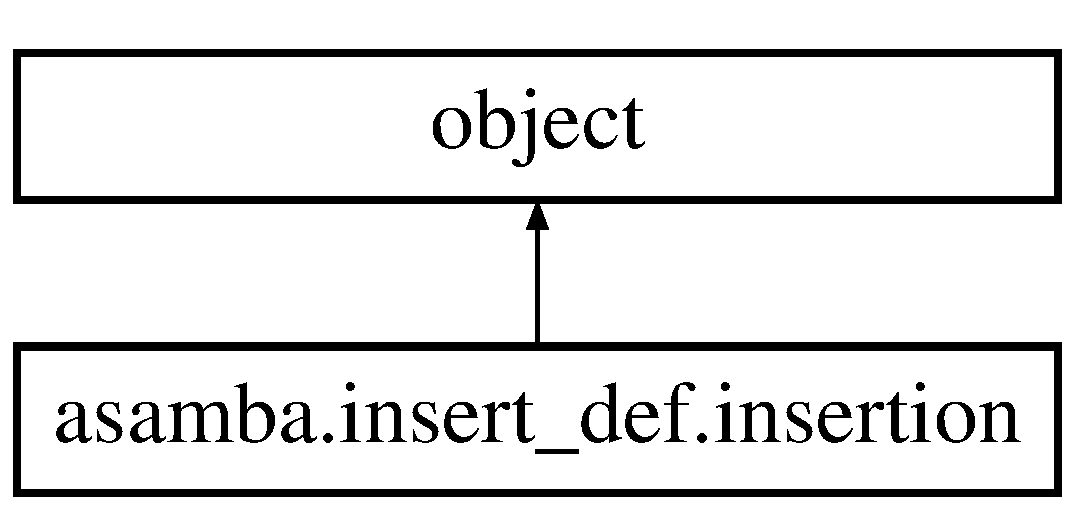
\includegraphics[height=2.000000cm]{classasamba_1_1insert__def_1_1insertion}
\end{center}
\end{figure}
\subsection*{Public Member Functions}
\begin{DoxyCompactItemize}
\item 
def \hyperlink{classasamba_1_1insert__def_1_1insertion_a0e4e59d72941182ec69091fc07d6cef0}{\+\_\+\+\_\+init\+\_\+\+\_\+} (self, table)
\item 
\mbox{\Hypertarget{classasamba_1_1insert__def_1_1insertion_a5b4f042cbf109ed685775bedce7b98b6}\label{classasamba_1_1insert__def_1_1insertion_a5b4f042cbf109ed685775bedce7b98b6}} 
def {\bfseries set\+\_\+table} (self, table)
\item 
\mbox{\Hypertarget{classasamba_1_1insert__def_1_1insertion_aeba8c7a346ddc819949ff194af0b4690}\label{classasamba_1_1insert__def_1_1insertion_aeba8c7a346ddc819949ff194af0b4690}} 
def {\bfseries get\+\_\+table} (self)
\end{DoxyCompactItemize}
\subsection*{Public Attributes}
\begin{DoxyCompactItemize}
\item 
\mbox{\Hypertarget{classasamba_1_1insert__def_1_1insertion_a47a62132fc8d77aee73fa5d08dbf6ce2}\label{classasamba_1_1insert__def_1_1insertion_a47a62132fc8d77aee73fa5d08dbf6ce2}} 
{\bfseries table}
\end{DoxyCompactItemize}


\subsection{Detailed Description}
\begin{DoxyVerb}Inserting data into the database tables
\end{DoxyVerb}
 

Definition at line 9 of file insert\+\_\+def.\+py.



\subsection{Constructor \& Destructor Documentation}
\mbox{\Hypertarget{classasamba_1_1insert__def_1_1insertion_a0e4e59d72941182ec69091fc07d6cef0}\label{classasamba_1_1insert__def_1_1insertion_a0e4e59d72941182ec69091fc07d6cef0}} 
\index{asamba\+::insert\+\_\+def\+::insertion@{asamba\+::insert\+\_\+def\+::insertion}!\+\_\+\+\_\+init\+\_\+\+\_\+@{\+\_\+\+\_\+init\+\_\+\+\_\+}}
\index{\+\_\+\+\_\+init\+\_\+\+\_\+@{\+\_\+\+\_\+init\+\_\+\+\_\+}!asamba\+::insert\+\_\+def\+::insertion@{asamba\+::insert\+\_\+def\+::insertion}}
\subsubsection{\texorpdfstring{\+\_\+\+\_\+init\+\_\+\+\_\+()}{\_\_init\_\_()}}
{\footnotesize\ttfamily def asamba.\+insert\+\_\+def.\+insertion.\+\_\+\+\_\+init\+\_\+\+\_\+ (\begin{DoxyParamCaption}\item[{}]{self,  }\item[{}]{table }\end{DoxyParamCaption})}

\begin{DoxyVerb}class constructor 

@param table: (default=None); insert data into one of the tables defined in the schema of the 
   database (grid.sql). The allowed values are:
   - tracks
   - models
   - rotation_rates
   - mode_types
   - modes
@type table: string
\end{DoxyVerb}
 

Definition at line 15 of file insert\+\_\+def.\+py.



The documentation for this class was generated from the following file\+:\begin{DoxyCompactItemize}
\item 
insert\+\_\+def.\+py\end{DoxyCompactItemize}

\hypertarget{classasamba_1_1interpolator_1_1interpolation}{}\section{asamba.\+interpolator.\+interpolation Class Reference}
\label{classasamba_1_1interpolator_1_1interpolation}\index{asamba.\+interpolator.\+interpolation@{asamba.\+interpolator.\+interpolation}}


\paragraph*{}

\subsection*{}

\subsection*{}

\subsection*{}

\subsection*{}

\subsection*{}

\subparagraph*{} 




Inheritance diagram for asamba.\+interpolator.\+interpolation\+:
% FIG 0


Collaboration diagram for asamba.\+interpolator.\+interpolation\+:
% FIG 1
\subsection*{Additional Inherited Members}


\subsection{Detailed Description}
\paragraph*{}

\subsection*{}

\subsection*{}

\subsection*{}

\subsection*{}

\subsection*{}

\subparagraph*{}

Definition at line 43 of file interpolator.\+py.



The documentation for this class was generated from the following file\+:\begin{DoxyCompactItemize}
\item 
interpolator.\+py\end{DoxyCompactItemize}

\hypertarget{classasamba_1_1star_1_1mode}{}\section{asamba.\+star.\+mode Class Reference}
\label{classasamba_1_1star_1_1mode}\index{asamba.\+star.\+mode@{asamba.\+star.\+mode}}


Inheritance diagram for asamba.\+star.\+mode\+:
% FIG 0


Collaboration diagram for asamba.\+star.\+mode\+:
% FIG 1
\subsection*{Public Member Functions}
\begin{DoxyCompactItemize}
\item 
\mbox{\Hypertarget{classasamba_1_1star_1_1mode_ac9526f60e2052a0f0fc55138a76217fc}\label{classasamba_1_1star_1_1mode_ac9526f60e2052a0f0fc55138a76217fc}} 
def {\bfseries \+\_\+\+\_\+init\+\_\+\+\_\+} (self)
\item 
\mbox{\Hypertarget{classasamba_1_1star_1_1mode_acd7157d9ec303f09579e24ba7d2638cc}\label{classasamba_1_1star_1_1mode_acd7157d9ec303f09579e24ba7d2638cc}} 
def \hyperlink{classasamba_1_1star_1_1mode_acd7157d9ec303f09579e24ba7d2638cc}{set} (self, attr, val)
\begin{DoxyCompactList}\small\item\em Setter. \end{DoxyCompactList}\item 
\mbox{\Hypertarget{classasamba_1_1star_1_1mode_a88d1239ec655f2bc03e5db88e170aad0}\label{classasamba_1_1star_1_1mode_a88d1239ec655f2bc03e5db88e170aad0}} 
def \hyperlink{classasamba_1_1star_1_1mode_a88d1239ec655f2bc03e5db88e170aad0}{get} (self, attr)
\begin{DoxyCompactList}\small\item\em Getter. \end{DoxyCompactList}\end{DoxyCompactItemize}
\subsection*{Public Attributes}
\begin{DoxyCompactItemize}
\item 
\mbox{\Hypertarget{classasamba_1_1star_1_1mode_a6003aa35ca504e83c244195dd0be0aa9}\label{classasamba_1_1star_1_1mode_a6003aa35ca504e83c244195dd0be0aa9}} 
{\bfseries freq}
\item 
\mbox{\Hypertarget{classasamba_1_1star_1_1mode_a04b08ed1bdbe5c67922016371873d078}\label{classasamba_1_1star_1_1mode_a04b08ed1bdbe5c67922016371873d078}} 
{\bfseries freq\+\_\+err}
\item 
\mbox{\Hypertarget{classasamba_1_1star_1_1mode_ac626ddf68f1b2574834e57caf9c46978}\label{classasamba_1_1star_1_1mode_ac626ddf68f1b2574834e57caf9c46978}} 
{\bfseries freq\+\_\+unit}
\item 
\mbox{\Hypertarget{classasamba_1_1star_1_1mode_a76a1b2601b1d958edca6b68435b9808a}\label{classasamba_1_1star_1_1mode_a76a1b2601b1d958edca6b68435b9808a}} 
{\bfseries amplitude}
\item 
\mbox{\Hypertarget{classasamba_1_1star_1_1mode_a0be493e05e856447886a4b93a63239ec}\label{classasamba_1_1star_1_1mode_a0be493e05e856447886a4b93a63239ec}} 
{\bfseries amplitude\+\_\+err}
\item 
\mbox{\Hypertarget{classasamba_1_1star_1_1mode_a439a154e6feeb8d745694ed4aa1e3b64}\label{classasamba_1_1star_1_1mode_a439a154e6feeb8d745694ed4aa1e3b64}} 
{\bfseries amplitude\+\_\+unit}
\item 
\mbox{\Hypertarget{classasamba_1_1star_1_1mode_a35d20dc954d4434a8904c23660b26fbb}\label{classasamba_1_1star_1_1mode_a35d20dc954d4434a8904c23660b26fbb}} 
{\bfseries n}
\item 
\mbox{\Hypertarget{classasamba_1_1star_1_1mode_a9527d01b6a59c7677d1026a2dc2a0f1a}\label{classasamba_1_1star_1_1mode_a9527d01b6a59c7677d1026a2dc2a0f1a}} 
{\bfseries l}
\item 
\mbox{\Hypertarget{classasamba_1_1star_1_1mode_a58fe1eb8496f48c0fd4195843eeaa717}\label{classasamba_1_1star_1_1mode_a58fe1eb8496f48c0fd4195843eeaa717}} 
{\bfseries m}
\item 
\mbox{\Hypertarget{classasamba_1_1star_1_1mode_a4f0ffe5b31745eeacac7016e1a80c06f}\label{classasamba_1_1star_1_1mode_a4f0ffe5b31745eeacac7016e1a80c06f}} 
{\bfseries p\+\_\+mode}
\item 
\mbox{\Hypertarget{classasamba_1_1star_1_1mode_a385b864ebec76029c6d7174725133c97}\label{classasamba_1_1star_1_1mode_a385b864ebec76029c6d7174725133c97}} 
{\bfseries g\+\_\+mode}
\item 
\mbox{\Hypertarget{classasamba_1_1star_1_1mode_a9b008393aa48f471d5949a6b63253d0e}\label{classasamba_1_1star_1_1mode_a9b008393aa48f471d5949a6b63253d0e}} 
{\bfseries in\+\_\+df}
\item 
\mbox{\Hypertarget{classasamba_1_1star_1_1mode_aeca13ebe6ebbd499f0d543bf57c3d133}\label{classasamba_1_1star_1_1mode_aeca13ebe6ebbd499f0d543bf57c3d133}} 
{\bfseries in\+\_\+dP}
\end{DoxyCompactItemize}


\subsection{Detailed Description}
\begin{DoxyVerb}Container for a single pulsation mode of a star. E.g. 

>>>from star import mode
>>>mode_1 = star.mode()
>>>mode_1.set('freq_unit', 'cd')

Note that the frequency unit is converted to "per day" if not already in this unit. This is convenient
because the typical frequencies of massive stars are around a day, and further feature normalization
is not really needed for frequencies. Whereas with Hertz, there is roughly a factor of 10^{-6} always
hanging around without any added value.
\end{DoxyVerb}
 

Definition at line 49 of file star.\+py.



The documentation for this class was generated from the following file\+:\begin{DoxyCompactItemize}
\item 
star.\+py\end{DoxyCompactItemize}

\hypertarget{classasamba_1_1var__def_1_1model}{}\section{asamba.\+var\+\_\+def.\+model Class Reference}
\label{classasamba_1_1var__def_1_1model}\index{asamba.\+var\+\_\+def.\+model@{asamba.\+var\+\_\+def.\+model}}
Inheritance diagram for asamba.\+var\+\_\+def.\+model\+:\begin{figure}[H]
\begin{center}
\leavevmode
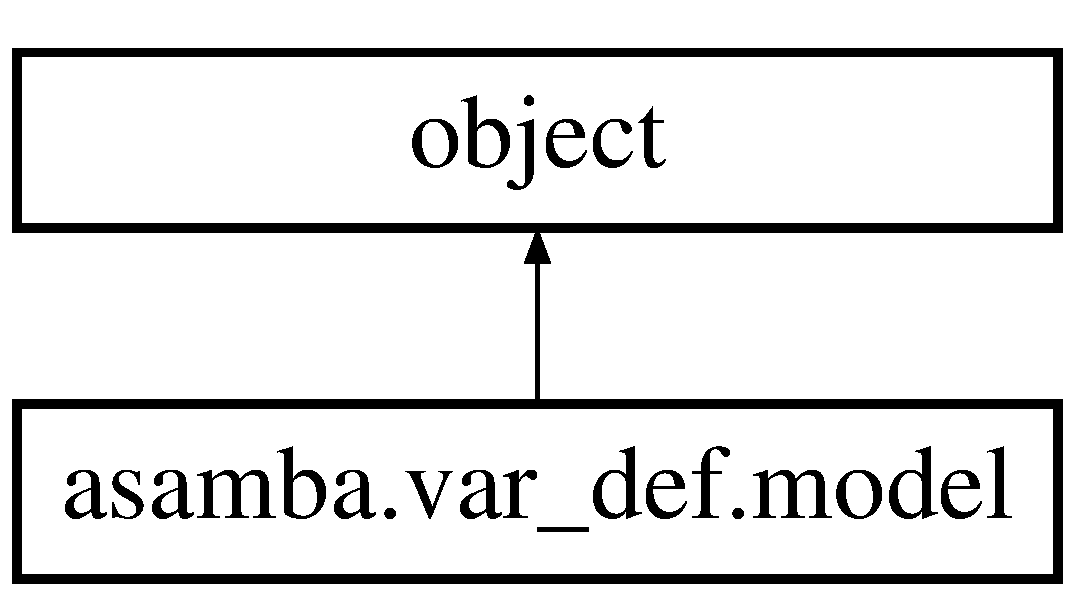
\includegraphics[height=2.000000cm]{classasamba_1_1var__def_1_1model}
\end{center}
\end{figure}
\subsection*{Public Member Functions}
\begin{DoxyCompactItemize}
\item 
def \hyperlink{classasamba_1_1var__def_1_1model_a6bb4340f0dd97b1311eb7b3e053de0c7}{\+\_\+\+\_\+init\+\_\+\+\_\+} (self)
\item 
\mbox{\Hypertarget{classasamba_1_1var__def_1_1model_a6a49d75a9ee4d9eed26b01023eff743f}\label{classasamba_1_1var__def_1_1model_a6a49d75a9ee4d9eed26b01023eff743f}} 
def {\bfseries \+\_\+\+\_\+enter\+\_\+\+\_\+} (self)
\item 
\mbox{\Hypertarget{classasamba_1_1var__def_1_1model_ab85d274fc5f0d3c17ee11b4d0e5fa739}\label{classasamba_1_1var__def_1_1model_ab85d274fc5f0d3c17ee11b4d0e5fa739}} 
def {\bfseries \+\_\+\+\_\+exit\+\_\+\+\_\+} (self, type, value, traceback)
\item 
\mbox{\Hypertarget{classasamba_1_1var__def_1_1model_a843e0624678507d02e9c8e6656563440}\label{classasamba_1_1var__def_1_1model_a843e0624678507d02e9c8e6656563440}} 
def {\bfseries set\+\_\+filename} (self, filename)
\item 
def \hyperlink{classasamba_1_1var__def_1_1model_a49205357c320bfe944bc1177b3d3a4ee}{set\+\_\+by\+\_\+dic} (self, dic)
\item 
def \hyperlink{classasamba_1_1var__def_1_1model_adf918a64e584736b39e108f4c705d413}{set} (self, attr, val)
\item 
def \hyperlink{classasamba_1_1var__def_1_1model_abc39be012825aa3842b694adc8a3b697}{get} (self, attr)
\end{DoxyCompactItemize}
\subsection*{Public Attributes}
\begin{DoxyCompactItemize}
\item 
\mbox{\Hypertarget{classasamba_1_1var__def_1_1model_a7f446ec899b32319f3d94edd2b58bd9b}\label{classasamba_1_1var__def_1_1model_a7f446ec899b32319f3d94edd2b58bd9b}} 
{\bfseries filename}
\item 
\mbox{\Hypertarget{classasamba_1_1var__def_1_1model_adcaaea581f15eb0a417ba14dc1dbd469}\label{classasamba_1_1var__def_1_1model_adcaaea581f15eb0a417ba14dc1dbd469}} 
{\bfseries M\+\_\+ini}
\item 
\mbox{\Hypertarget{classasamba_1_1var__def_1_1model_a228653ff26586f56d170110b6a1bae9e}\label{classasamba_1_1var__def_1_1model_a228653ff26586f56d170110b6a1bae9e}} 
{\bfseries fov}
\item 
\mbox{\Hypertarget{classasamba_1_1var__def_1_1model_aa7735590fccf115cdf588ecf9b901e7a}\label{classasamba_1_1var__def_1_1model_aa7735590fccf115cdf588ecf9b901e7a}} 
{\bfseries Z}
\item 
\mbox{\Hypertarget{classasamba_1_1var__def_1_1model_a6610ed4fb47670aa6c50a11137aa5ff0}\label{classasamba_1_1var__def_1_1model_a6610ed4fb47670aa6c50a11137aa5ff0}} 
{\bfseries logD}
\item 
\mbox{\Hypertarget{classasamba_1_1var__def_1_1model_afb499ea021f0715d03ee4eae7257d069}\label{classasamba_1_1var__def_1_1model_afb499ea021f0715d03ee4eae7257d069}} 
{\bfseries Xc}
\item 
\mbox{\Hypertarget{classasamba_1_1var__def_1_1model_acbdfd50972b2be45157b5061090ef6fb}\label{classasamba_1_1var__def_1_1model_acbdfd50972b2be45157b5061090ef6fb}} 
{\bfseries model\+\_\+number}
\item 
\mbox{\Hypertarget{classasamba_1_1var__def_1_1model_a595c517e1ba4c0379612c1dd4c15ea3a}\label{classasamba_1_1var__def_1_1model_a595c517e1ba4c0379612c1dd4c15ea3a}} 
{\bfseries star\+\_\+mass}
\item 
\mbox{\Hypertarget{classasamba_1_1var__def_1_1model_ad0f82c868451b18b2760b26667d92042}\label{classasamba_1_1var__def_1_1model_ad0f82c868451b18b2760b26667d92042}} 
{\bfseries radius}
\item 
\mbox{\Hypertarget{classasamba_1_1var__def_1_1model_a4a5ff84f75ab5e93982efc52b0883695}\label{classasamba_1_1var__def_1_1model_a4a5ff84f75ab5e93982efc52b0883695}} 
{\bfseries log\+\_\+\+Teff}
\item 
\mbox{\Hypertarget{classasamba_1_1var__def_1_1model_a12a3022f1c8b82b18de38b7c246fa0a1}\label{classasamba_1_1var__def_1_1model_a12a3022f1c8b82b18de38b7c246fa0a1}} 
{\bfseries log\+\_\+g}
\item 
\mbox{\Hypertarget{classasamba_1_1var__def_1_1model_ae8559bdbbfe023a12885bf0528c844b4}\label{classasamba_1_1var__def_1_1model_ae8559bdbbfe023a12885bf0528c844b4}} 
{\bfseries log\+\_\+L}
\item 
\mbox{\Hypertarget{classasamba_1_1var__def_1_1model_a196451876cf67192b4980a1d170188a0}\label{classasamba_1_1var__def_1_1model_a196451876cf67192b4980a1d170188a0}} 
{\bfseries log\+\_\+\+Ledd}
\item 
\mbox{\Hypertarget{classasamba_1_1var__def_1_1model_a7a1b278c4333f2c70c4b36b2d0618f57}\label{classasamba_1_1var__def_1_1model_a7a1b278c4333f2c70c4b36b2d0618f57}} 
{\bfseries log\+\_\+abs\+\_\+mdot}
\item 
\mbox{\Hypertarget{classasamba_1_1var__def_1_1model_aeb874391bc02337bb252df4131a44f69}\label{classasamba_1_1var__def_1_1model_aeb874391bc02337bb252df4131a44f69}} 
{\bfseries mass\+\_\+conv\+\_\+core}
\item 
\mbox{\Hypertarget{classasamba_1_1var__def_1_1model_aecc53b1e7ddfe75a57b38cd026190cff}\label{classasamba_1_1var__def_1_1model_aecc53b1e7ddfe75a57b38cd026190cff}} 
{\bfseries star\+\_\+age}
\item 
\mbox{\Hypertarget{classasamba_1_1var__def_1_1model_a5bf9613482f45cd559d4e4d1d500e6dd}\label{classasamba_1_1var__def_1_1model_a5bf9613482f45cd559d4e4d1d500e6dd}} 
{\bfseries dynamic\+\_\+timescale}
\item 
\mbox{\Hypertarget{classasamba_1_1var__def_1_1model_a85430ca777cd918b5d9706e53973c7d7}\label{classasamba_1_1var__def_1_1model_a85430ca777cd918b5d9706e53973c7d7}} 
{\bfseries kh\+\_\+timescale}
\item 
\mbox{\Hypertarget{classasamba_1_1var__def_1_1model_aa82a3dbf2e78944336dfbe4aac58372f}\label{classasamba_1_1var__def_1_1model_aa82a3dbf2e78944336dfbe4aac58372f}} 
{\bfseries nuc\+\_\+timescale}
\item 
\mbox{\Hypertarget{classasamba_1_1var__def_1_1model_acf97982d5b5d6f89eb1b8e97f8c575c3}\label{classasamba_1_1var__def_1_1model_acf97982d5b5d6f89eb1b8e97f8c575c3}} 
{\bfseries log\+\_\+center\+\_\+T}
\item 
\mbox{\Hypertarget{classasamba_1_1var__def_1_1model_ad67c7cb475708e5127223d1c34c2c1cb}\label{classasamba_1_1var__def_1_1model_ad67c7cb475708e5127223d1c34c2c1cb}} 
{\bfseries log\+\_\+center\+\_\+\+Rho}
\item 
\mbox{\Hypertarget{classasamba_1_1var__def_1_1model_aba2088929e7800fdc9d0de01e6ab6d9c}\label{classasamba_1_1var__def_1_1model_aba2088929e7800fdc9d0de01e6ab6d9c}} 
{\bfseries log\+\_\+center\+\_\+P}
\item 
\mbox{\Hypertarget{classasamba_1_1var__def_1_1model_af9962144c40864f73c042c429b10839f}\label{classasamba_1_1var__def_1_1model_af9962144c40864f73c042c429b10839f}} 
{\bfseries center\+\_\+h1}
\item 
\mbox{\Hypertarget{classasamba_1_1var__def_1_1model_a2751b8ccca82916eea8a17e8f18d6d27}\label{classasamba_1_1var__def_1_1model_a2751b8ccca82916eea8a17e8f18d6d27}} 
{\bfseries center\+\_\+h2}
\item 
\mbox{\Hypertarget{classasamba_1_1var__def_1_1model_ac0a66fc6d2f27e036d3b47eaa33c9f70}\label{classasamba_1_1var__def_1_1model_ac0a66fc6d2f27e036d3b47eaa33c9f70}} 
{\bfseries center\+\_\+he3}
\item 
\mbox{\Hypertarget{classasamba_1_1var__def_1_1model_a820f8b110f3003e2c896b1118b3134c8}\label{classasamba_1_1var__def_1_1model_a820f8b110f3003e2c896b1118b3134c8}} 
{\bfseries center\+\_\+he4}
\item 
\mbox{\Hypertarget{classasamba_1_1var__def_1_1model_a29b8d90d7bae1eee48780b513b0f8682}\label{classasamba_1_1var__def_1_1model_a29b8d90d7bae1eee48780b513b0f8682}} 
{\bfseries center\+\_\+c12}
\item 
\mbox{\Hypertarget{classasamba_1_1var__def_1_1model_ac49a0d92275c8bd871fbdf154bb2d052}\label{classasamba_1_1var__def_1_1model_ac49a0d92275c8bd871fbdf154bb2d052}} 
{\bfseries center\+\_\+c13}
\item 
\mbox{\Hypertarget{classasamba_1_1var__def_1_1model_a0b9e70cebb2c3b7e6aa777e0fb2fb0ec}\label{classasamba_1_1var__def_1_1model_a0b9e70cebb2c3b7e6aa777e0fb2fb0ec}} 
{\bfseries center\+\_\+n14}
\item 
\mbox{\Hypertarget{classasamba_1_1var__def_1_1model_a06ee1546e5c914d6b498cc966e60a86d}\label{classasamba_1_1var__def_1_1model_a06ee1546e5c914d6b498cc966e60a86d}} 
{\bfseries center\+\_\+n15}
\item 
\mbox{\Hypertarget{classasamba_1_1var__def_1_1model_a216d637d0aec7193ec7af98eed0a491b}\label{classasamba_1_1var__def_1_1model_a216d637d0aec7193ec7af98eed0a491b}} 
{\bfseries center\+\_\+o16}
\item 
\mbox{\Hypertarget{classasamba_1_1var__def_1_1model_a9ffa1edb64394586e1058b6ef1ee6aab}\label{classasamba_1_1var__def_1_1model_a9ffa1edb64394586e1058b6ef1ee6aab}} 
{\bfseries center\+\_\+o18}
\item 
\mbox{\Hypertarget{classasamba_1_1var__def_1_1model_ae0ea2ae397ebb60964a16f790faf7f77}\label{classasamba_1_1var__def_1_1model_ae0ea2ae397ebb60964a16f790faf7f77}} 
{\bfseries center\+\_\+ne20}
\item 
\mbox{\Hypertarget{classasamba_1_1var__def_1_1model_a94808168e5c693c40b104fd466224a3f}\label{classasamba_1_1var__def_1_1model_a94808168e5c693c40b104fd466224a3f}} 
{\bfseries center\+\_\+ne22}
\item 
\mbox{\Hypertarget{classasamba_1_1var__def_1_1model_ad6948b987ffc0dd5c67692f5d626937f}\label{classasamba_1_1var__def_1_1model_ad6948b987ffc0dd5c67692f5d626937f}} 
{\bfseries center\+\_\+mg24}
\item 
\mbox{\Hypertarget{classasamba_1_1var__def_1_1model_a96301181558a35827f4cde6b0cd0d6d9}\label{classasamba_1_1var__def_1_1model_a96301181558a35827f4cde6b0cd0d6d9}} 
{\bfseries surface\+\_\+h1}
\item 
\mbox{\Hypertarget{classasamba_1_1var__def_1_1model_aa8447776b737b0d8f3e35787e3183aeb}\label{classasamba_1_1var__def_1_1model_aa8447776b737b0d8f3e35787e3183aeb}} 
{\bfseries surface\+\_\+h2}
\item 
\mbox{\Hypertarget{classasamba_1_1var__def_1_1model_a7905f672e05a1029f3d4978a3b8c4764}\label{classasamba_1_1var__def_1_1model_a7905f672e05a1029f3d4978a3b8c4764}} 
{\bfseries surface\+\_\+he3}
\item 
\mbox{\Hypertarget{classasamba_1_1var__def_1_1model_a820bce606a97fd2c6c702d27c89aa7f5}\label{classasamba_1_1var__def_1_1model_a820bce606a97fd2c6c702d27c89aa7f5}} 
{\bfseries surface\+\_\+he4}
\item 
\mbox{\Hypertarget{classasamba_1_1var__def_1_1model_a37d6dd9fc1cb98197bbb7431859950a1}\label{classasamba_1_1var__def_1_1model_a37d6dd9fc1cb98197bbb7431859950a1}} 
{\bfseries surface\+\_\+c12}
\item 
\mbox{\Hypertarget{classasamba_1_1var__def_1_1model_aed75477a276f93a7710e7aacca8e896d}\label{classasamba_1_1var__def_1_1model_aed75477a276f93a7710e7aacca8e896d}} 
{\bfseries surface\+\_\+c13}
\item 
\mbox{\Hypertarget{classasamba_1_1var__def_1_1model_a2f0c0cdf8513c6b91d4732fc67a01dad}\label{classasamba_1_1var__def_1_1model_a2f0c0cdf8513c6b91d4732fc67a01dad}} 
{\bfseries surface\+\_\+n14}
\item 
\mbox{\Hypertarget{classasamba_1_1var__def_1_1model_acc757d3f0b962dea407de51727789139}\label{classasamba_1_1var__def_1_1model_acc757d3f0b962dea407de51727789139}} 
{\bfseries surface\+\_\+n15}
\item 
\mbox{\Hypertarget{classasamba_1_1var__def_1_1model_ad953d1b76003f5fb3b674b2c1815ac25}\label{classasamba_1_1var__def_1_1model_ad953d1b76003f5fb3b674b2c1815ac25}} 
{\bfseries surface\+\_\+o16}
\item 
\mbox{\Hypertarget{classasamba_1_1var__def_1_1model_abd2e78697969380859082a86e50c629c}\label{classasamba_1_1var__def_1_1model_abd2e78697969380859082a86e50c629c}} 
{\bfseries surface\+\_\+o18}
\item 
\mbox{\Hypertarget{classasamba_1_1var__def_1_1model_a1ce265f2cf172aa5ebc97eaf42259bd0}\label{classasamba_1_1var__def_1_1model_a1ce265f2cf172aa5ebc97eaf42259bd0}} 
{\bfseries surface\+\_\+ne20}
\item 
\mbox{\Hypertarget{classasamba_1_1var__def_1_1model_adf29e9cc8a8427331f7df56512d76fea}\label{classasamba_1_1var__def_1_1model_adf29e9cc8a8427331f7df56512d76fea}} 
{\bfseries surface\+\_\+ne22}
\item 
\mbox{\Hypertarget{classasamba_1_1var__def_1_1model_a9f011955c5572b497df636a640e3917f}\label{classasamba_1_1var__def_1_1model_a9f011955c5572b497df636a640e3917f}} 
{\bfseries surface\+\_\+mg24}
\item 
\mbox{\Hypertarget{classasamba_1_1var__def_1_1model_a37d39a5c929fd18efe6cf4142f45793d}\label{classasamba_1_1var__def_1_1model_a37d39a5c929fd18efe6cf4142f45793d}} 
{\bfseries delta\+\_\+nu}
\item 
\mbox{\Hypertarget{classasamba_1_1var__def_1_1model_a4efb4f186a74e1645e73e5a8afdf4428}\label{classasamba_1_1var__def_1_1model_a4efb4f186a74e1645e73e5a8afdf4428}} 
{\bfseries nu\+\_\+max}
\item 
\mbox{\Hypertarget{classasamba_1_1var__def_1_1model_aaa395e3c6bcd3bc72453abc2a1a80364}\label{classasamba_1_1var__def_1_1model_aaa395e3c6bcd3bc72453abc2a1a80364}} 
{\bfseries acoustic\+\_\+cutoff}
\item 
\mbox{\Hypertarget{classasamba_1_1var__def_1_1model_a20969a3fff51673d4eb006e4111322bc}\label{classasamba_1_1var__def_1_1model_a20969a3fff51673d4eb006e4111322bc}} 
{\bfseries delta\+\_\+\+Pg}
\item 
\mbox{\Hypertarget{classasamba_1_1var__def_1_1model_a3b9effa2eea2d62aedabf6c559233b69}\label{classasamba_1_1var__def_1_1model_a3b9effa2eea2d62aedabf6c559233b69}} 
{\bfseries Mbol}
\item 
\mbox{\Hypertarget{classasamba_1_1var__def_1_1model_a23e5c98b118cf406f76f449ec6f49240}\label{classasamba_1_1var__def_1_1model_a23e5c98b118cf406f76f449ec6f49240}} 
{\bfseries bcv}
\item 
\mbox{\Hypertarget{classasamba_1_1var__def_1_1model_a99d65f26f006ee193851105490f52ce7}\label{classasamba_1_1var__def_1_1model_a99d65f26f006ee193851105490f52ce7}} 
{\bfseries U\+\_\+B}
\item 
\mbox{\Hypertarget{classasamba_1_1var__def_1_1model_a630f76bf4eab180e6774337326190bbc}\label{classasamba_1_1var__def_1_1model_a630f76bf4eab180e6774337326190bbc}} 
{\bfseries B\+\_\+V}
\item 
\mbox{\Hypertarget{classasamba_1_1var__def_1_1model_a064204fa102f196d0843fab7039e58bb}\label{classasamba_1_1var__def_1_1model_a064204fa102f196d0843fab7039e58bb}} 
{\bfseries V\+\_\+R}
\item 
\mbox{\Hypertarget{classasamba_1_1var__def_1_1model_ab96d9c3adc9350939a1765a804604ef4}\label{classasamba_1_1var__def_1_1model_ab96d9c3adc9350939a1765a804604ef4}} 
{\bfseries V\+\_\+I}
\item 
\mbox{\Hypertarget{classasamba_1_1var__def_1_1model_abb4127412ab183c8dab374d1cda52aad}\label{classasamba_1_1var__def_1_1model_abb4127412ab183c8dab374d1cda52aad}} 
{\bfseries V\+\_\+K}
\item 
\mbox{\Hypertarget{classasamba_1_1var__def_1_1model_a987931b2eb09b177d4eebe854c782a51}\label{classasamba_1_1var__def_1_1model_a987931b2eb09b177d4eebe854c782a51}} 
{\bfseries R\+\_\+I}
\item 
\mbox{\Hypertarget{classasamba_1_1var__def_1_1model_a5ca38d549f192609afce700cf5b1c4f3}\label{classasamba_1_1var__def_1_1model_a5ca38d549f192609afce700cf5b1c4f3}} 
{\bfseries I\+\_\+K}
\item 
\mbox{\Hypertarget{classasamba_1_1var__def_1_1model_abd5f63d4c1b0e05cd202d55f6cb658fb}\label{classasamba_1_1var__def_1_1model_abd5f63d4c1b0e05cd202d55f6cb658fb}} 
{\bfseries J\+\_\+H}
\item 
\mbox{\Hypertarget{classasamba_1_1var__def_1_1model_a597ddf7dcd5310edc3aef5fc4b3ef91b}\label{classasamba_1_1var__def_1_1model_a597ddf7dcd5310edc3aef5fc4b3ef91b}} 
{\bfseries H\+\_\+K}
\item 
\mbox{\Hypertarget{classasamba_1_1var__def_1_1model_ac96b6bb1341f39b2d4d54d1a3b520ebb}\label{classasamba_1_1var__def_1_1model_ac96b6bb1341f39b2d4d54d1a3b520ebb}} 
{\bfseries K\+\_\+L}
\item 
\mbox{\Hypertarget{classasamba_1_1var__def_1_1model_a13f1539423c716924a11e1bcf7ccc069}\label{classasamba_1_1var__def_1_1model_a13f1539423c716924a11e1bcf7ccc069}} 
{\bfseries J\+\_\+K}
\item 
\mbox{\Hypertarget{classasamba_1_1var__def_1_1model_a9ca962db67ce685bf2442e172a8cd8cd}\label{classasamba_1_1var__def_1_1model_a9ca962db67ce685bf2442e172a8cd8cd}} 
{\bfseries J\+\_\+L}
\item 
\mbox{\Hypertarget{classasamba_1_1var__def_1_1model_ab6601fec6d9887cf3b5b16aa3c75eef2}\label{classasamba_1_1var__def_1_1model_ab6601fec6d9887cf3b5b16aa3c75eef2}} 
{\bfseries J\+\_\+\+Lp}
\item 
\mbox{\Hypertarget{classasamba_1_1var__def_1_1model_a350a6ef82b4e052b39eebd4c88d0a30b}\label{classasamba_1_1var__def_1_1model_a350a6ef82b4e052b39eebd4c88d0a30b}} 
{\bfseries K\+\_\+M}
\end{DoxyCompactItemize}


\subsection{Detailed Description}
\begin{DoxyVerb}The class that encapsulates the properties of each of MESA output model files which serve as inputs
to GYRE.
\end{DoxyVerb}
 

Definition at line 298 of file var\+\_\+def.\+py.



\subsection{Constructor \& Destructor Documentation}
\mbox{\Hypertarget{classasamba_1_1var__def_1_1model_a6bb4340f0dd97b1311eb7b3e053de0c7}\label{classasamba_1_1var__def_1_1model_a6bb4340f0dd97b1311eb7b3e053de0c7}} 
\index{asamba\+::var\+\_\+def\+::model@{asamba\+::var\+\_\+def\+::model}!\+\_\+\+\_\+init\+\_\+\+\_\+@{\+\_\+\+\_\+init\+\_\+\+\_\+}}
\index{\+\_\+\+\_\+init\+\_\+\+\_\+@{\+\_\+\+\_\+init\+\_\+\+\_\+}!asamba\+::var\+\_\+def\+::model@{asamba\+::var\+\_\+def\+::model}}
\subsubsection{\texorpdfstring{\+\_\+\+\_\+init\+\_\+\+\_\+()}{\_\_init\_\_()}}
{\footnotesize\ttfamily def asamba.\+var\+\_\+def.\+model.\+\_\+\+\_\+init\+\_\+\+\_\+ (\begin{DoxyParamCaption}\item[{}]{self }\end{DoxyParamCaption})}

\begin{DoxyVerb}constructor of the class
\end{DoxyVerb}
 

Definition at line 303 of file var\+\_\+def.\+py.



\subsection{Member Function Documentation}
\mbox{\Hypertarget{classasamba_1_1var__def_1_1model_abc39be012825aa3842b694adc8a3b697}\label{classasamba_1_1var__def_1_1model_abc39be012825aa3842b694adc8a3b697}} 
\index{asamba\+::var\+\_\+def\+::model@{asamba\+::var\+\_\+def\+::model}!get@{get}}
\index{get@{get}!asamba\+::var\+\_\+def\+::model@{asamba\+::var\+\_\+def\+::model}}
\subsubsection{\texorpdfstring{get()}{get()}}
{\footnotesize\ttfamily def asamba.\+var\+\_\+def.\+model.\+get (\begin{DoxyParamCaption}\item[{}]{self,  }\item[{}]{attr }\end{DoxyParamCaption})}

\begin{DoxyVerb}General-purpose method to get the value of a canonical attribute of the object
E.g.

>>>val = a_model.get('age')

@param attr: the name of the available attribute of the class
@type attr: string
@return: the value of the attribute
@rtype: float
\end{DoxyVerb}
 

Definition at line 445 of file var\+\_\+def.\+py.

\mbox{\Hypertarget{classasamba_1_1var__def_1_1model_adf918a64e584736b39e108f4c705d413}\label{classasamba_1_1var__def_1_1model_adf918a64e584736b39e108f4c705d413}} 
\index{asamba\+::var\+\_\+def\+::model@{asamba\+::var\+\_\+def\+::model}!set@{set}}
\index{set@{set}!asamba\+::var\+\_\+def\+::model@{asamba\+::var\+\_\+def\+::model}}
\subsubsection{\texorpdfstring{set()}{set()}}
{\footnotesize\ttfamily def asamba.\+var\+\_\+def.\+model.\+set (\begin{DoxyParamCaption}\item[{}]{self,  }\item[{}]{attr,  }\item[{}]{val }\end{DoxyParamCaption})}

\begin{DoxyVerb}Set the value of the specific attribute "attr" of the model object
\end{DoxyVerb}
 

Definition at line 433 of file var\+\_\+def.\+py.

\mbox{\Hypertarget{classasamba_1_1var__def_1_1model_a49205357c320bfe944bc1177b3d3a4ee}\label{classasamba_1_1var__def_1_1model_a49205357c320bfe944bc1177b3d3a4ee}} 
\index{asamba\+::var\+\_\+def\+::model@{asamba\+::var\+\_\+def\+::model}!set\+\_\+by\+\_\+dic@{set\+\_\+by\+\_\+dic}}
\index{set\+\_\+by\+\_\+dic@{set\+\_\+by\+\_\+dic}!asamba\+::var\+\_\+def\+::model@{asamba\+::var\+\_\+def\+::model}}
\subsubsection{\texorpdfstring{set\+\_\+by\+\_\+dic()}{set\_by\_dic()}}
{\footnotesize\ttfamily def asamba.\+var\+\_\+def.\+model.\+set\+\_\+by\+\_\+dic (\begin{DoxyParamCaption}\item[{}]{self,  }\item[{}]{dic }\end{DoxyParamCaption})}

\begin{DoxyVerb}Since the "model" class has many attributes, instead of writing a setter for all 
attributes manually (exhaustive), we pass the attribute values through a dictionary.
This is a general-purpose interface to set the "canonical" attributes of the "model"
class. E.g. 

>>> a_model.set_by_dic({'Teff':10125.0, 'log_g':4.128, 'center_018':1.4509e-5})

@param self: an instance of the model class
@type self: object
@param dic: a dictionary containing the attributes to be set in the model, e.g.
@type dic: dict
\end{DoxyVerb}
 

Definition at line 404 of file var\+\_\+def.\+py.



The documentation for this class was generated from the following file\+:\begin{DoxyCompactItemize}
\item 
var\+\_\+def.\+py\end{DoxyCompactItemize}

\hypertarget{classasamba_1_1backend_1_1_modelling_session}{}\section{asamba.\+backend.\+Modelling\+Session Class Reference}
\label{classasamba_1_1backend_1_1_modelling_session}\index{asamba.\+backend.\+Modelling\+Session@{asamba.\+backend.\+Modelling\+Session}}


U S E R -\/ C O N T R O L L E D P A R A M E T E R S \+: B A C K E N D O B J E C T S T H A T D O T H E R E A L W O R K.  




Inheritance diagram for asamba.\+backend.\+Modelling\+Session\+:
% FIG 0


Collaboration diagram for asamba.\+backend.\+Modelling\+Session\+:
% FIG 1
\subsection*{Public Member Functions}
\begin{DoxyCompactItemize}
\item 
def \hyperlink{classasamba_1_1backend_1_1_modelling_session_a4d7e25887ba7c8af5ae303b2dc63191d}{\+\_\+\+\_\+init\+\_\+\+\_\+} (self)
\item 
def \hyperlink{classasamba_1_1backend_1_1_modelling_session_a83549fd610225e6edea77914b0f65f30}{set} (self, attr, val)
\item 
def \hyperlink{classasamba_1_1backend_1_1_modelling_session_a32588cc6e0b3869d3d5ef688953599d2}{get} (self, attr)
\end{DoxyCompactItemize}
\subsection*{Additional Inherited Members}


\subsection{Detailed Description}
U S E R -\/ C O N T R O L L E D P A R A M E T E R S \+: B A C K E N D O B J E C T S T H A T D O T H E R E A L W O R K. 

\begin{DoxyVerb}The ModellingSession is a derived class from the underlying modules in the package. 
Concretely, the parent classes which are used here are below, in the following "Method
Resolution Order (MRO)":

  - interpolator.interpolation
  - artificial_neural_network.neural_net
  - sampler.sampling
  - star.star

With the bundling of the above classes, we create a derived class which takes care of 
the observatinal data, the theoretical models in the database, the interface between 
the underlying routine and the PostgreSQL database, and the high-level machine learning
analysis machinery.
\end{DoxyVerb}
 

Definition at line 27 of file backend.\+py.



\subsection{Constructor \& Destructor Documentation}
\mbox{\Hypertarget{classasamba_1_1backend_1_1_modelling_session_a4d7e25887ba7c8af5ae303b2dc63191d}\label{classasamba_1_1backend_1_1_modelling_session_a4d7e25887ba7c8af5ae303b2dc63191d}} 
\index{asamba\+::backend\+::\+Modelling\+Session@{asamba\+::backend\+::\+Modelling\+Session}!\+\_\+\+\_\+init\+\_\+\+\_\+@{\+\_\+\+\_\+init\+\_\+\+\_\+}}
\index{\+\_\+\+\_\+init\+\_\+\+\_\+@{\+\_\+\+\_\+init\+\_\+\+\_\+}!asamba\+::backend\+::\+Modelling\+Session@{asamba\+::backend\+::\+Modelling\+Session}}
\subsubsection{\texorpdfstring{\+\_\+\+\_\+init\+\_\+\+\_\+()}{\_\_init\_\_()}}
{\footnotesize\ttfamily def asamba.\+backend.\+Modelling\+Session.\+\_\+\+\_\+init\+\_\+\+\_\+ (\begin{DoxyParamCaption}\item[{}]{self }\end{DoxyParamCaption})}

\begin{DoxyVerb}Constructor \end{DoxyVerb}
 

Definition at line 44 of file backend.\+py.



\subsection{Member Function Documentation}
\mbox{\Hypertarget{classasamba_1_1backend_1_1_modelling_session_a32588cc6e0b3869d3d5ef688953599d2}\label{classasamba_1_1backend_1_1_modelling_session_a32588cc6e0b3869d3d5ef688953599d2}} 
\index{asamba\+::backend\+::\+Modelling\+Session@{asamba\+::backend\+::\+Modelling\+Session}!get@{get}}
\index{get@{get}!asamba\+::backend\+::\+Modelling\+Session@{asamba\+::backend\+::\+Modelling\+Session}}
\subsubsection{\texorpdfstring{get()}{get()}}
{\footnotesize\ttfamily def asamba.\+backend.\+Modelling\+Session.\+get (\begin{DoxyParamCaption}\item[{}]{self,  }\item[{}]{attr }\end{DoxyParamCaption})}

\begin{DoxyVerb}Getter \end{DoxyVerb}
 

Definition at line 52 of file backend.\+py.

Here is the caller graph for this function\+:
% FIG 2
\mbox{\Hypertarget{classasamba_1_1backend_1_1_modelling_session_a83549fd610225e6edea77914b0f65f30}\label{classasamba_1_1backend_1_1_modelling_session_a83549fd610225e6edea77914b0f65f30}} 
\index{asamba\+::backend\+::\+Modelling\+Session@{asamba\+::backend\+::\+Modelling\+Session}!set@{set}}
\index{set@{set}!asamba\+::backend\+::\+Modelling\+Session@{asamba\+::backend\+::\+Modelling\+Session}}
\subsubsection{\texorpdfstring{set()}{set()}}
{\footnotesize\ttfamily def asamba.\+backend.\+Modelling\+Session.\+set (\begin{DoxyParamCaption}\item[{}]{self,  }\item[{}]{attr,  }\item[{}]{val }\end{DoxyParamCaption})}

\begin{DoxyVerb}Setter \end{DoxyVerb}
 

Definition at line 48 of file backend.\+py.

Here is the caller graph for this function\+:
% FIG 3


The documentation for this class was generated from the following file\+:\begin{DoxyCompactItemize}
\item 
backend.\+py\end{DoxyCompactItemize}

\hypertarget{classasamba_1_1var__def_1_1models}{}\section{asamba.\+var\+\_\+def.\+models Class Reference}
\label{classasamba_1_1var__def_1_1models}\index{asamba.\+var\+\_\+def.\+models@{asamba.\+var\+\_\+def.\+models}}


Inheritance diagram for asamba.\+var\+\_\+def.\+models\+:
% FIG 0


Collaboration diagram for asamba.\+var\+\_\+def.\+models\+:
% FIG 1
\subsection*{Public Member Functions}
\begin{DoxyCompactItemize}
\item 
def \hyperlink{classasamba_1_1var__def_1_1models_a21b6a3b0d85fafe41208098a03fcf7ab}{\+\_\+\+\_\+init\+\_\+\+\_\+} (self, dir\+\_\+repos)
\item 
\mbox{\Hypertarget{classasamba_1_1var__def_1_1models_afcc52884c26aac2e9aa85eecc38119b6}\label{classasamba_1_1var__def_1_1models_afcc52884c26aac2e9aa85eecc38119b6}} 
def {\bfseries \+\_\+\+\_\+enter\+\_\+\+\_\+} (self)
\item 
\mbox{\Hypertarget{classasamba_1_1var__def_1_1models_ad3911bafbf1ffbe6c7357ce0762b47c8}\label{classasamba_1_1var__def_1_1models_ad3911bafbf1ffbe6c7357ce0762b47c8}} 
def {\bfseries \+\_\+\+\_\+exit\+\_\+\+\_\+} (self, type, value, traceback)
\item 
\mbox{\Hypertarget{classasamba_1_1var__def_1_1models_a0701c4b198d774b5a54aa378e25779f6}\label{classasamba_1_1var__def_1_1models_a0701c4b198d774b5a54aa378e25779f6}} 
def {\bfseries set\+\_\+model\+\_\+search\+\_\+pattern} (self, model\+\_\+search\+\_\+pattern)
\item 
\mbox{\Hypertarget{classasamba_1_1var__def_1_1models_a2827d4182c5d3a85bf559daaca81bec3}\label{classasamba_1_1var__def_1_1models_a2827d4182c5d3a85bf559daaca81bec3}} 
def {\bfseries set\+\_\+model\+\_\+extension} (self, model\+\_\+extension)
\item 
\mbox{\Hypertarget{classasamba_1_1var__def_1_1models_a0f23ccd6f783e5c3e5878d6efd5a5fd5}\label{classasamba_1_1var__def_1_1models_a0f23ccd6f783e5c3e5878d6efd5a5fd5}} 
def {\bfseries set\+\_\+n\+\_\+models} (self, n\+\_\+models)
\item 
\mbox{\Hypertarget{classasamba_1_1var__def_1_1models_a6d42985357f164d32ae57a6b38b267e7}\label{classasamba_1_1var__def_1_1models_a6d42985357f164d32ae57a6b38b267e7}} 
def {\bfseries set\+\_\+list\+\_\+filenames} (self, list\+\_\+filenames)
\item 
\mbox{\Hypertarget{classasamba_1_1var__def_1_1models_af251a31d212a3f448a482d7f455e4efe}\label{classasamba_1_1var__def_1_1models_af251a31d212a3f448a482d7f455e4efe}} 
def {\bfseries set\+\_\+list\+\_\+models} (self, list\+\_\+models)
\item 
def \hyperlink{classasamba_1_1var__def_1_1models_ae0babd86feff61275e38952a7cc23282}{find\+\_\+list\+\_\+filenames} (self)
\item 
\mbox{\Hypertarget{classasamba_1_1var__def_1_1models_a803340c120565c5c7efc4caf0eab9785}\label{classasamba_1_1var__def_1_1models_a803340c120565c5c7efc4caf0eab9785}} 
def {\bfseries sort\+\_\+list\+\_\+filenames} (self)
\item 
\mbox{\Hypertarget{classasamba_1_1var__def_1_1models_ae7c4bf74c3b026d2b02afd17a0d8958e}\label{classasamba_1_1var__def_1_1models_ae7c4bf74c3b026d2b02afd17a0d8958e}} 
def {\bfseries get\+\_\+model\+\_\+search\+\_\+pattern} (self)
\item 
\mbox{\Hypertarget{classasamba_1_1var__def_1_1models_acd68787862f1bc189b591cdc7b1f8317}\label{classasamba_1_1var__def_1_1models_acd68787862f1bc189b591cdc7b1f8317}} 
def {\bfseries get\+\_\+model\+\_\+extension} (self)
\item 
\mbox{\Hypertarget{classasamba_1_1var__def_1_1models_af2265e679ad70a301f49597023f74af1}\label{classasamba_1_1var__def_1_1models_af2265e679ad70a301f49597023f74af1}} 
def {\bfseries get\+\_\+list\+\_\+filenames} (self)
\item 
\mbox{\Hypertarget{classasamba_1_1var__def_1_1models_a0d42ee8bfa9d99a37768e31f843f5a9f}\label{classasamba_1_1var__def_1_1models_a0d42ee8bfa9d99a37768e31f843f5a9f}} 
def {\bfseries get\+\_\+list\+\_\+models} (self)
\item 
\mbox{\Hypertarget{classasamba_1_1var__def_1_1models_a610f2b866ecb89f6541e30c461e825bd}\label{classasamba_1_1var__def_1_1models_a610f2b866ecb89f6541e30c461e825bd}} 
def {\bfseries get\+\_\+n\+\_\+models} (self)
\end{DoxyCompactItemize}
\subsection*{Public Attributes}
\begin{DoxyCompactItemize}
\item 
\mbox{\Hypertarget{classasamba_1_1var__def_1_1models_a44661e2a402b05c80da5c9387d030a0d}\label{classasamba_1_1var__def_1_1models_a44661e2a402b05c80da5c9387d030a0d}} 
{\bfseries dir\+\_\+repos}
\item 
\mbox{\Hypertarget{classasamba_1_1var__def_1_1models_a3d6a55a38b5b43d6c0780ed4c26f885f}\label{classasamba_1_1var__def_1_1models_a3d6a55a38b5b43d6c0780ed4c26f885f}} 
{\bfseries model\+\_\+search\+\_\+pattern}
\item 
\mbox{\Hypertarget{classasamba_1_1var__def_1_1models_ac27eceb3a2d44515e86329f0f36ccebd}\label{classasamba_1_1var__def_1_1models_ac27eceb3a2d44515e86329f0f36ccebd}} 
{\bfseries model\+\_\+extension}
\item 
\mbox{\Hypertarget{classasamba_1_1var__def_1_1models_a56ca32e9e5fc6ced55d70e4e4e102ea2}\label{classasamba_1_1var__def_1_1models_a56ca32e9e5fc6ced55d70e4e4e102ea2}} 
{\bfseries n\+\_\+models}
\item 
\mbox{\Hypertarget{classasamba_1_1var__def_1_1models_a4807b6490e5b7afe8377880762049b86}\label{classasamba_1_1var__def_1_1models_a4807b6490e5b7afe8377880762049b86}} 
{\bfseries list\+\_\+filenames}
\item 
\mbox{\Hypertarget{classasamba_1_1var__def_1_1models_a7716492752231f81909b728d633f4494}\label{classasamba_1_1var__def_1_1models_a7716492752231f81909b728d633f4494}} 
{\bfseries list\+\_\+models}
\end{DoxyCompactItemize}


\subsection{Detailed Description}
\begin{DoxyVerb}An agglomeration (container) of the objects from the "model" class
\end{DoxyVerb}
 

Definition at line 464 of file var\+\_\+def.\+py.



\subsection{Constructor \& Destructor Documentation}
\mbox{\Hypertarget{classasamba_1_1var__def_1_1models_a21b6a3b0d85fafe41208098a03fcf7ab}\label{classasamba_1_1var__def_1_1models_a21b6a3b0d85fafe41208098a03fcf7ab}} 
\index{asamba\+::var\+\_\+def\+::models@{asamba\+::var\+\_\+def\+::models}!\+\_\+\+\_\+init\+\_\+\+\_\+@{\+\_\+\+\_\+init\+\_\+\+\_\+}}
\index{\+\_\+\+\_\+init\+\_\+\+\_\+@{\+\_\+\+\_\+init\+\_\+\+\_\+}!asamba\+::var\+\_\+def\+::models@{asamba\+::var\+\_\+def\+::models}}
\subsubsection{\texorpdfstring{\+\_\+\+\_\+init\+\_\+\+\_\+()}{\_\_init\_\_()}}
{\footnotesize\ttfamily def asamba.\+var\+\_\+def.\+models.\+\_\+\+\_\+init\+\_\+\+\_\+ (\begin{DoxyParamCaption}\item[{}]{self,  }\item[{}]{dir\+\_\+repos }\end{DoxyParamCaption})}

\begin{DoxyVerb}Constructor of the class. It can be instantiated by specifying the full path to the repository. 
E.g.

>>>many_models = var_def.models('/home/user/projects/mygrid')\end{DoxyVerb}
 

Definition at line 468 of file var\+\_\+def.\+py.



\subsection{Member Function Documentation}
\mbox{\Hypertarget{classasamba_1_1var__def_1_1models_ae0babd86feff61275e38952a7cc23282}\label{classasamba_1_1var__def_1_1models_ae0babd86feff61275e38952a7cc23282}} 
\index{asamba\+::var\+\_\+def\+::models@{asamba\+::var\+\_\+def\+::models}!find\+\_\+list\+\_\+filenames@{find\+\_\+list\+\_\+filenames}}
\index{find\+\_\+list\+\_\+filenames@{find\+\_\+list\+\_\+filenames}!asamba\+::var\+\_\+def\+::models@{asamba\+::var\+\_\+def\+::models}}
\subsubsection{\texorpdfstring{find\+\_\+list\+\_\+filenames()}{find\_list\_filenames()}}
{\footnotesize\ttfamily def asamba.\+var\+\_\+def.\+models.\+find\+\_\+list\+\_\+filenames (\begin{DoxyParamCaption}\item[{}]{self }\end{DoxyParamCaption})}

\begin{DoxyVerb}Find present models on the disk that match the search pattern.

@param dir_repos: the full path to the repository where the files sit, e.g. '/home/user/mygrid'
@type dir_repos: string
@param model_search_pattern: the search pattern for globbing the available model files. e.g.
  'M*/gyre_in/*'
@type model_search_pattern: string
\end{DoxyVerb}
 

Definition at line 518 of file var\+\_\+def.\+py.

Here is the call graph for this function\+:
% FIG 2


The documentation for this class was generated from the following file\+:\begin{DoxyCompactItemize}
\item 
var\+\_\+def.\+py\end{DoxyCompactItemize}

\hypertarget{classasamba_1_1var__def_1_1modes}{}\section{asamba.\+var\+\_\+def.\+modes Class Reference}
\label{classasamba_1_1var__def_1_1modes}\index{asamba.\+var\+\_\+def.\+modes@{asamba.\+var\+\_\+def.\+modes}}
Inheritance diagram for asamba.\+var\+\_\+def.\+modes\+:\begin{figure}[H]
\begin{center}
\leavevmode
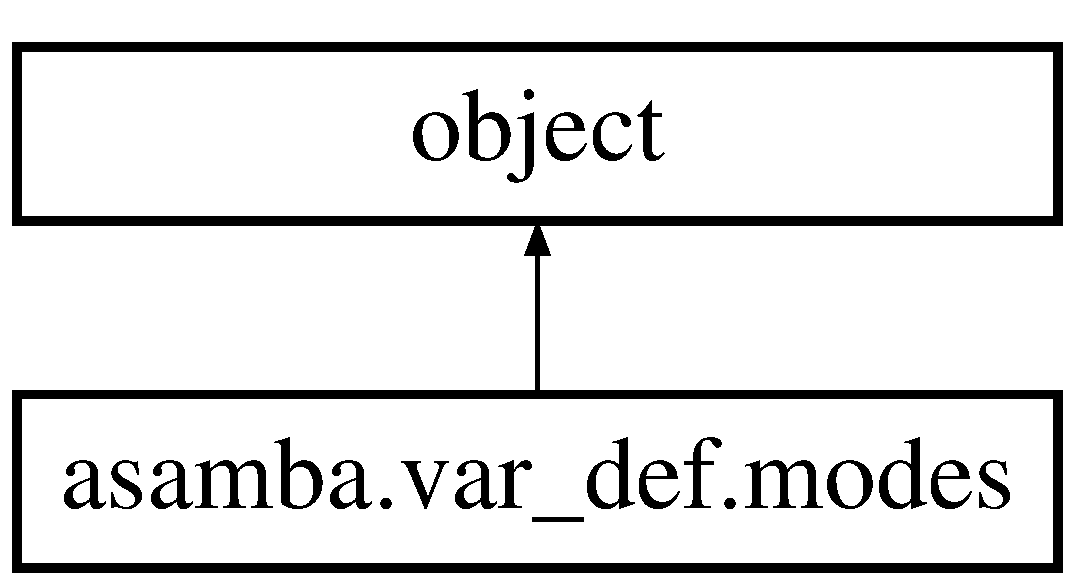
\includegraphics[height=2.000000cm]{classasamba_1_1var__def_1_1modes}
\end{center}
\end{figure}
\subsection*{Public Member Functions}
\begin{DoxyCompactItemize}
\item 
def \hyperlink{classasamba_1_1var__def_1_1modes_a3e7e2e2e01dadeb07002bde1f8e35ac9}{\+\_\+\+\_\+init\+\_\+\+\_\+} (self)
\item 
\mbox{\Hypertarget{classasamba_1_1var__def_1_1modes_ae15778f02288da4abc131dfd5d0af151}\label{classasamba_1_1var__def_1_1modes_ae15778f02288da4abc131dfd5d0af151}} 
def {\bfseries \+\_\+\+\_\+enter\+\_\+\+\_\+} (self)
\item 
\mbox{\Hypertarget{classasamba_1_1var__def_1_1modes_a928762de62f113e943da5a711c546397}\label{classasamba_1_1var__def_1_1modes_a928762de62f113e943da5a711c546397}} 
def {\bfseries \+\_\+\+\_\+exit\+\_\+\+\_\+} (self, type, value, traceback)
\item 
def \hyperlink{classasamba_1_1var__def_1_1modes_a68e3175f54a123a371a9e5345b2cfe6e}{set} (self, attr, val)
\item 
def \hyperlink{classasamba_1_1var__def_1_1modes_a2d9b87e9cdfe54142627a502476bb868}{set\+\_\+by\+\_\+dic} (self, dic)
\end{DoxyCompactItemize}
\subsection*{Public Attributes}
\begin{DoxyCompactItemize}
\item 
\mbox{\Hypertarget{classasamba_1_1var__def_1_1modes_a2093f0cd80f29a1a028ec5201b871a6b}\label{classasamba_1_1var__def_1_1modes_a2093f0cd80f29a1a028ec5201b871a6b}} 
{\bfseries l}
\item 
\mbox{\Hypertarget{classasamba_1_1var__def_1_1modes_a9856db104cea06faea5507c026d7456d}\label{classasamba_1_1var__def_1_1modes_a9856db104cea06faea5507c026d7456d}} 
{\bfseries l\+\_\+0}
\item 
\mbox{\Hypertarget{classasamba_1_1var__def_1_1modes_a3f1460a74f06ddd3ad3f6d2b04011990}\label{classasamba_1_1var__def_1_1modes_a3f1460a74f06ddd3ad3f6d2b04011990}} 
{\bfseries m}
\item 
\mbox{\Hypertarget{classasamba_1_1var__def_1_1modes_a049923aad4828ee504fe88c3433b5179}\label{classasamba_1_1var__def_1_1modes_a049923aad4828ee504fe88c3433b5179}} 
{\bfseries n\+\_\+pg}
\item 
\mbox{\Hypertarget{classasamba_1_1var__def_1_1modes_a315e3825dcd065519c40354f882996a2}\label{classasamba_1_1var__def_1_1modes_a315e3825dcd065519c40354f882996a2}} 
{\bfseries n\+\_\+p}
\item 
\mbox{\Hypertarget{classasamba_1_1var__def_1_1modes_ae04b49b400db1f19440c11d5c6dca97c}\label{classasamba_1_1var__def_1_1modes_ae04b49b400db1f19440c11d5c6dca97c}} 
{\bfseries n\+\_\+g}
\item 
\mbox{\Hypertarget{classasamba_1_1var__def_1_1modes_a5a5b1f5584312652e3f8228f3b09104e}\label{classasamba_1_1var__def_1_1modes_a5a5b1f5584312652e3f8228f3b09104e}} 
{\bfseries omega}
\item 
\mbox{\Hypertarget{classasamba_1_1var__def_1_1modes_a503f5d883f3e486b21bfdd65e28acc40}\label{classasamba_1_1var__def_1_1modes_a503f5d883f3e486b21bfdd65e28acc40}} 
{\bfseries omega\+\_\+int}
\item 
\mbox{\Hypertarget{classasamba_1_1var__def_1_1modes_a0bb3770ae61ef8991a72f9c9343f123f}\label{classasamba_1_1var__def_1_1modes_a0bb3770ae61ef8991a72f9c9343f123f}} 
{\bfseries freq}
\item 
\mbox{\Hypertarget{classasamba_1_1var__def_1_1modes_a965f0466a8526e517679d5c24802a24c}\label{classasamba_1_1var__def_1_1modes_a965f0466a8526e517679d5c24802a24c}} 
{\bfseries freq\+\_\+units}
\item 
\mbox{\Hypertarget{classasamba_1_1var__def_1_1modes_addefacd0beff89624f6b101487c07053}\label{classasamba_1_1var__def_1_1modes_addefacd0beff89624f6b101487c07053}} 
{\bfseries f\+\_\+T}
\item 
\mbox{\Hypertarget{classasamba_1_1var__def_1_1modes_a0446ae4e25b0bc111660021aeeddfaeb}\label{classasamba_1_1var__def_1_1modes_a0446ae4e25b0bc111660021aeeddfaeb}} 
{\bfseries f\+\_\+g}
\item 
\mbox{\Hypertarget{classasamba_1_1var__def_1_1modes_a5ab0a6c679b5fe0a2ef749ca02db0ce1}\label{classasamba_1_1var__def_1_1modes_a5ab0a6c679b5fe0a2ef749ca02db0ce1}} 
{\bfseries psi\+\_\+T}
\item 
\mbox{\Hypertarget{classasamba_1_1var__def_1_1modes_a857885889483b7efaabdba673988d06a}\label{classasamba_1_1var__def_1_1modes_a857885889483b7efaabdba673988d06a}} 
{\bfseries psi\+\_\+g}
\item 
\mbox{\Hypertarget{classasamba_1_1var__def_1_1modes_aece047ae82078bf02f331ebe40124d34}\label{classasamba_1_1var__def_1_1modes_aece047ae82078bf02f331ebe40124d34}} 
{\bfseries beta}
\item 
\mbox{\Hypertarget{classasamba_1_1var__def_1_1modes_a461002b089de4c644a8a8c74907e376c}\label{classasamba_1_1var__def_1_1modes_a461002b089de4c644a8a8c74907e376c}} 
{\bfseries E}
\item 
\mbox{\Hypertarget{classasamba_1_1var__def_1_1modes_aaa940309c979e1c55b5c3a12051e124b}\label{classasamba_1_1var__def_1_1modes_aaa940309c979e1c55b5c3a12051e124b}} 
{\bfseries E\+\_\+norm}
\item 
\mbox{\Hypertarget{classasamba_1_1var__def_1_1modes_aef72630d13c4198990b42b8831540493}\label{classasamba_1_1var__def_1_1modes_aef72630d13c4198990b42b8831540493}} 
{\bfseries W}
\item 
\mbox{\Hypertarget{classasamba_1_1var__def_1_1modes_a512b154b76afae26d1f25c1f2a4a8e93}\label{classasamba_1_1var__def_1_1modes_a512b154b76afae26d1f25c1f2a4a8e93}} 
{\bfseries M\+\_\+star}
\item 
\mbox{\Hypertarget{classasamba_1_1var__def_1_1modes_a7e9113df2353b7f6c57ce32e39f56732}\label{classasamba_1_1var__def_1_1modes_a7e9113df2353b7f6c57ce32e39f56732}} 
{\bfseries R\+\_\+star}
\item 
\mbox{\Hypertarget{classasamba_1_1var__def_1_1modes_a9c0d2a9fc9eef5766b649417eb58e2cf}\label{classasamba_1_1var__def_1_1modes_a9c0d2a9fc9eef5766b649417eb58e2cf}} 
{\bfseries L\+\_\+star}
\item 
\mbox{\Hypertarget{classasamba_1_1var__def_1_1modes_a94306b8bd1065650f930683a1961f419}\label{classasamba_1_1var__def_1_1modes_a94306b8bd1065650f930683a1961f419}} 
{\bfseries n\+\_\+poly}
\item 
\mbox{\Hypertarget{classasamba_1_1var__def_1_1modes_a9d50a2b5b16b35e9456c9665c90a2a0c}\label{classasamba_1_1var__def_1_1modes_a9d50a2b5b16b35e9456c9665c90a2a0c}} 
{\bfseries W\+\_\+eps}
\item 
\mbox{\Hypertarget{classasamba_1_1var__def_1_1modes_a3508c1f71eaee3c3f7345281fb50cdb5}\label{classasamba_1_1var__def_1_1modes_a3508c1f71eaee3c3f7345281fb50cdb5}} 
{\bfseries n}
\item 
\mbox{\Hypertarget{classasamba_1_1var__def_1_1modes_a972fb47ae5dc9de526dbef405e95ba55}\label{classasamba_1_1var__def_1_1modes_a972fb47ae5dc9de526dbef405e95ba55}} 
{\bfseries x}
\item 
\mbox{\Hypertarget{classasamba_1_1var__def_1_1modes_af2fef28086bbc7532c37f474be35e687}\label{classasamba_1_1var__def_1_1modes_af2fef28086bbc7532c37f474be35e687}} 
{\bfseries V}
\item 
\mbox{\Hypertarget{classasamba_1_1var__def_1_1modes_a151552b279817e247e57e8c943396132}\label{classasamba_1_1var__def_1_1modes_a151552b279817e247e57e8c943396132}} 
{\bfseries As}
\item 
\mbox{\Hypertarget{classasamba_1_1var__def_1_1modes_a8d563f144b094064ac089b6fbe8bf077}\label{classasamba_1_1var__def_1_1modes_a8d563f144b094064ac089b6fbe8bf077}} 
{\bfseries U}
\item 
\mbox{\Hypertarget{classasamba_1_1var__def_1_1modes_a88c73aa4fe2a386d809a68fef24dc570}\label{classasamba_1_1var__def_1_1modes_a88c73aa4fe2a386d809a68fef24dc570}} 
{\bfseries c\+\_\+1}
\item 
\mbox{\Hypertarget{classasamba_1_1var__def_1_1modes_ac336f62c2ddfea23ee3f97b052ea45a1}\label{classasamba_1_1var__def_1_1modes_ac336f62c2ddfea23ee3f97b052ea45a1}} 
{\bfseries Gamma\+\_\+1}
\item 
\mbox{\Hypertarget{classasamba_1_1var__def_1_1modes_ac1ba7ac8da40fdc968a58d7bb3f49dd4}\label{classasamba_1_1var__def_1_1modes_ac1ba7ac8da40fdc968a58d7bb3f49dd4}} 
{\bfseries nabla\+\_\+ad}
\item 
\mbox{\Hypertarget{classasamba_1_1var__def_1_1modes_ae4de903aeff6ae2839defc01ce64180e}\label{classasamba_1_1var__def_1_1modes_ae4de903aeff6ae2839defc01ce64180e}} 
{\bfseries delta}
\item 
\mbox{\Hypertarget{classasamba_1_1var__def_1_1modes_a2bfc19077f3145a8d0d28234cb92c8e4}\label{classasamba_1_1var__def_1_1modes_a2bfc19077f3145a8d0d28234cb92c8e4}} 
{\bfseries Omega\+\_\+rot}
\item 
\mbox{\Hypertarget{classasamba_1_1var__def_1_1modes_ac6be1074329428a22e6973b0d0eef1ca}\label{classasamba_1_1var__def_1_1modes_ac6be1074329428a22e6973b0d0eef1ca}} 
{\bfseries xi\+\_\+r}
\item 
\mbox{\Hypertarget{classasamba_1_1var__def_1_1modes_a862fdbeecdd319acbaeba8279ef9a380}\label{classasamba_1_1var__def_1_1modes_a862fdbeecdd319acbaeba8279ef9a380}} 
{\bfseries xi\+\_\+h}
\item 
\mbox{\Hypertarget{classasamba_1_1var__def_1_1modes_a1d69a00f18ece3bc657b32b9ac011e8b}\label{classasamba_1_1var__def_1_1modes_a1d69a00f18ece3bc657b32b9ac011e8b}} 
{\bfseries Yt\+\_\+1}
\item 
\mbox{\Hypertarget{classasamba_1_1var__def_1_1modes_abb734c06ea84841e1a5842dcc05712ac}\label{classasamba_1_1var__def_1_1modes_abb734c06ea84841e1a5842dcc05712ac}} 
{\bfseries Yt\+\_\+2}
\item 
\mbox{\Hypertarget{classasamba_1_1var__def_1_1modes_aacb76836e40bf785c6f3eae7b56117cc}\label{classasamba_1_1var__def_1_1modes_aacb76836e40bf785c6f3eae7b56117cc}} 
{\bfseries eul\+\_\+phi}
\item 
\mbox{\Hypertarget{classasamba_1_1var__def_1_1modes_a4f36aa955926c8ee328cbbf33adca044}\label{classasamba_1_1var__def_1_1modes_a4f36aa955926c8ee328cbbf33adca044}} 
{\bfseries deul\+\_\+phi}
\item 
\mbox{\Hypertarget{classasamba_1_1var__def_1_1modes_a7fc498962a482fdf2ef2e1b906e85673}\label{classasamba_1_1var__def_1_1modes_a7fc498962a482fdf2ef2e1b906e85673}} 
{\bfseries eul\+\_\+p}
\item 
\mbox{\Hypertarget{classasamba_1_1var__def_1_1modes_a7781d50183e4a321a17083353cbaf10a}\label{classasamba_1_1var__def_1_1modes_a7781d50183e4a321a17083353cbaf10a}} 
{\bfseries eul\+\_\+rho}
\item 
\mbox{\Hypertarget{classasamba_1_1var__def_1_1modes_af7ab994988e9f4d61b20caa7704cfb99}\label{classasamba_1_1var__def_1_1modes_af7ab994988e9f4d61b20caa7704cfb99}} 
{\bfseries eul\+\_\+T}
\item 
\mbox{\Hypertarget{classasamba_1_1var__def_1_1modes_af6c68dd7df0849a6e223247b8e3ec83c}\label{classasamba_1_1var__def_1_1modes_af6c68dd7df0849a6e223247b8e3ec83c}} 
{\bfseries lag\+\_\+S}
\item 
\mbox{\Hypertarget{classasamba_1_1var__def_1_1modes_a5dda57c1b22eb6c56ea8fc8a834c3b65}\label{classasamba_1_1var__def_1_1modes_a5dda57c1b22eb6c56ea8fc8a834c3b65}} 
{\bfseries lag\+\_\+L}
\item 
\mbox{\Hypertarget{classasamba_1_1var__def_1_1modes_a18bca3299f192c62a1e4eab6e28c1464}\label{classasamba_1_1var__def_1_1modes_a18bca3299f192c62a1e4eab6e28c1464}} 
{\bfseries lag\+\_\+p}
\item 
\mbox{\Hypertarget{classasamba_1_1var__def_1_1modes_a68219f38443384c2bfb10c276dc9d59f}\label{classasamba_1_1var__def_1_1modes_a68219f38443384c2bfb10c276dc9d59f}} 
{\bfseries lag\+\_\+rho}
\item 
\mbox{\Hypertarget{classasamba_1_1var__def_1_1modes_aec2e4fba1afedf72b036d50eee3e4a1b}\label{classasamba_1_1var__def_1_1modes_aec2e4fba1afedf72b036d50eee3e4a1b}} 
{\bfseries lag\+\_\+T}
\item 
\mbox{\Hypertarget{classasamba_1_1var__def_1_1modes_a10b707282fb263330acfec479322fbd2}\label{classasamba_1_1var__def_1_1modes_a10b707282fb263330acfec479322fbd2}} 
{\bfseries d\+E\+\_\+dx}
\item 
\mbox{\Hypertarget{classasamba_1_1var__def_1_1modes_a42a7001673078d7893d9a4c774053670}\label{classasamba_1_1var__def_1_1modes_a42a7001673078d7893d9a4c774053670}} 
{\bfseries d\+W\+\_\+eps\+\_\+dx}
\item 
\mbox{\Hypertarget{classasamba_1_1var__def_1_1modes_abe005002c5bca2330d87bb6a9c3c88d9}\label{classasamba_1_1var__def_1_1modes_abe005002c5bca2330d87bb6a9c3c88d9}} 
{\bfseries d\+W\+\_\+dx}
\item 
\mbox{\Hypertarget{classasamba_1_1var__def_1_1modes_a6f008dc0452b46a62fa2838db16a817f}\label{classasamba_1_1var__def_1_1modes_a6f008dc0452b46a62fa2838db16a817f}} 
{\bfseries prop\+\_\+type}
\item 
\mbox{\Hypertarget{classasamba_1_1var__def_1_1modes_aa941b7ceaf1e3719fa0d96feb2026910}\label{classasamba_1_1var__def_1_1modes_aa941b7ceaf1e3719fa0d96feb2026910}} 
{\bfseries K}
\item 
\mbox{\Hypertarget{classasamba_1_1var__def_1_1modes_a82118ff0203cda5aa81ffebe050480be}\label{classasamba_1_1var__def_1_1modes_a82118ff0203cda5aa81ffebe050480be}} 
{\bfseries M\+\_\+r}
\item 
\mbox{\Hypertarget{classasamba_1_1var__def_1_1modes_a6651bc41dfad320052400385a813611e}\label{classasamba_1_1var__def_1_1modes_a6651bc41dfad320052400385a813611e}} 
{\bfseries p}
\item 
\mbox{\Hypertarget{classasamba_1_1var__def_1_1modes_a34e06af2e02dfa6a7e7fc4a6576d8d1e}\label{classasamba_1_1var__def_1_1modes_a34e06af2e02dfa6a7e7fc4a6576d8d1e}} 
{\bfseries rho}
\item 
\mbox{\Hypertarget{classasamba_1_1var__def_1_1modes_a8faeea4050695e5b297464a746179e3b}\label{classasamba_1_1var__def_1_1modes_a8faeea4050695e5b297464a746179e3b}} 
{\bfseries T}
\item 
\mbox{\Hypertarget{classasamba_1_1var__def_1_1modes_ab46084e01587c79201da7cd2799d22fd}\label{classasamba_1_1var__def_1_1modes_ab46084e01587c79201da7cd2799d22fd}} 
{\bfseries F\+\_\+j}
\item 
\mbox{\Hypertarget{classasamba_1_1var__def_1_1modes_a17b8a735886d4aaa988dcad54a4d7cdf}\label{classasamba_1_1var__def_1_1modes_a17b8a735886d4aaa988dcad54a4d7cdf}} 
{\bfseries div\+\_\+\+F\+\_\+j}
\item 
\mbox{\Hypertarget{classasamba_1_1var__def_1_1modes_a632181ff0c8c224e89404a3d44a3f190}\label{classasamba_1_1var__def_1_1modes_a632181ff0c8c224e89404a3d44a3f190}} 
{\bfseries freq\+\_\+rot}
\item 
\mbox{\Hypertarget{classasamba_1_1var__def_1_1modes_addb3760a10df298392bca09f06aa8c1e}\label{classasamba_1_1var__def_1_1modes_addb3760a10df298392bca09f06aa8c1e}} 
{\bfseries freq\+\_\+crit}
\item 
\mbox{\Hypertarget{classasamba_1_1var__def_1_1modes_a39e79bc979d3b545f6c4a98093d0c2bc}\label{classasamba_1_1var__def_1_1modes_a39e79bc979d3b545f6c4a98093d0c2bc}} 
{\bfseries eta\+\_\+rot}
\item 
\mbox{\Hypertarget{classasamba_1_1var__def_1_1modes_acea37e3fc94676be4a39dc13fe306e0e}\label{classasamba_1_1var__def_1_1modes_acea37e3fc94676be4a39dc13fe306e0e}} 
{\bfseries omega\+\_\+rot}
\item 
\mbox{\Hypertarget{classasamba_1_1var__def_1_1modes_acf54b56da47442b3ada6abcb7da78aa1}\label{classasamba_1_1var__def_1_1modes_acf54b56da47442b3ada6abcb7da78aa1}} 
{\bfseries label}
\end{DoxyCompactItemize}


\subsection{Detailed Description}
\begin{DoxyVerb}This is a light-weight container for the GYRE outputs. All attriutes corresponding to the summary
files or the eigenfunction files are available. The fields are initiated to "None" to keep the default
volume of the objects minimal.
\end{DoxyVerb}
 

Definition at line 582 of file var\+\_\+def.\+py.



\subsection{Constructor \& Destructor Documentation}
\mbox{\Hypertarget{classasamba_1_1var__def_1_1modes_a3e7e2e2e01dadeb07002bde1f8e35ac9}\label{classasamba_1_1var__def_1_1modes_a3e7e2e2e01dadeb07002bde1f8e35ac9}} 
\index{asamba\+::var\+\_\+def\+::modes@{asamba\+::var\+\_\+def\+::modes}!\+\_\+\+\_\+init\+\_\+\+\_\+@{\+\_\+\+\_\+init\+\_\+\+\_\+}}
\index{\+\_\+\+\_\+init\+\_\+\+\_\+@{\+\_\+\+\_\+init\+\_\+\+\_\+}!asamba\+::var\+\_\+def\+::modes@{asamba\+::var\+\_\+def\+::modes}}
\subsubsection{\texorpdfstring{\+\_\+\+\_\+init\+\_\+\+\_\+()}{\_\_init\_\_()}}
{\footnotesize\ttfamily def asamba.\+var\+\_\+def.\+modes.\+\_\+\+\_\+init\+\_\+\+\_\+ (\begin{DoxyParamCaption}\item[{}]{self }\end{DoxyParamCaption})}

\begin{DoxyVerb}Constructor of the class. The attributes are based on the GYRE v.4.4, and the list of attributes 
are availble here: <https://bitbucket.org/rhdtownsend/gyre/wiki/Output%20Files%20(4.4)>
The data types after allocation is either integer, float, string
\end{DoxyVerb}
 

Definition at line 589 of file var\+\_\+def.\+py.



\subsection{Member Function Documentation}
\mbox{\Hypertarget{classasamba_1_1var__def_1_1modes_a68e3175f54a123a371a9e5345b2cfe6e}\label{classasamba_1_1var__def_1_1modes_a68e3175f54a123a371a9e5345b2cfe6e}} 
\index{asamba\+::var\+\_\+def\+::modes@{asamba\+::var\+\_\+def\+::modes}!set@{set}}
\index{set@{set}!asamba\+::var\+\_\+def\+::modes@{asamba\+::var\+\_\+def\+::modes}}
\subsubsection{\texorpdfstring{set()}{set()}}
{\footnotesize\ttfamily def asamba.\+var\+\_\+def.\+modes.\+set (\begin{DoxyParamCaption}\item[{}]{self,  }\item[{}]{attr,  }\item[{}]{val }\end{DoxyParamCaption})}

\begin{DoxyVerb}Set the value of an attribute
\end{DoxyVerb}
 

Definition at line 677 of file var\+\_\+def.\+py.

\mbox{\Hypertarget{classasamba_1_1var__def_1_1modes_a2d9b87e9cdfe54142627a502476bb868}\label{classasamba_1_1var__def_1_1modes_a2d9b87e9cdfe54142627a502476bb868}} 
\index{asamba\+::var\+\_\+def\+::modes@{asamba\+::var\+\_\+def\+::modes}!set\+\_\+by\+\_\+dic@{set\+\_\+by\+\_\+dic}}
\index{set\+\_\+by\+\_\+dic@{set\+\_\+by\+\_\+dic}!asamba\+::var\+\_\+def\+::modes@{asamba\+::var\+\_\+def\+::modes}}
\subsubsection{\texorpdfstring{set\+\_\+by\+\_\+dic()}{set\_by\_dic()}}
{\footnotesize\ttfamily def asamba.\+var\+\_\+def.\+modes.\+set\+\_\+by\+\_\+dic (\begin{DoxyParamCaption}\item[{}]{self,  }\item[{}]{dic }\end{DoxyParamCaption})}

\begin{DoxyVerb}Set the attributes of the object through the available items (key, values) in the passed 
dictionary. This is to minimize the number of necessary calls to the "set()" method.

@param self: An instance of the modes class
@type self: object
@param dic: A dictionary containing the contents of the GYRE output files
@type dic: dictionary
\end{DoxyVerb}
 

Definition at line 687 of file var\+\_\+def.\+py.



The documentation for this class was generated from the following file\+:\begin{DoxyCompactItemize}
\item 
var\+\_\+def.\+py\end{DoxyCompactItemize}

\hypertarget{classasamba_1_1star_1_1modes}{}\section{asamba.\+star.\+modes Class Reference}
\label{classasamba_1_1star_1_1modes}\index{asamba.\+star.\+modes@{asamba.\+star.\+modes}}


Inheritance diagram for asamba.\+star.\+modes\+:
% FIG 0


Collaboration diagram for asamba.\+star.\+modes\+:
% FIG 1
\subsection*{Public Member Functions}
\begin{DoxyCompactItemize}
\item 
\mbox{\Hypertarget{classasamba_1_1star_1_1modes_abce4d33b22e4f51db250c3e384591be6}\label{classasamba_1_1star_1_1modes_abce4d33b22e4f51db250c3e384591be6}} 
def {\bfseries \+\_\+\+\_\+init\+\_\+\+\_\+} (self)
\item 
\mbox{\Hypertarget{classasamba_1_1star_1_1modes_a86f1dd21b0af24cc60d521fbeb391ef8}\label{classasamba_1_1star_1_1modes_a86f1dd21b0af24cc60d521fbeb391ef8}} 
def \hyperlink{classasamba_1_1star_1_1modes_a86f1dd21b0af24cc60d521fbeb391ef8}{set} (self, attr, val)
\begin{DoxyCompactList}\small\item\em Setter. \end{DoxyCompactList}\item 
\mbox{\Hypertarget{classasamba_1_1star_1_1modes_a4bf25d680e466f4e888b3a63df76281d}\label{classasamba_1_1star_1_1modes_a4bf25d680e466f4e888b3a63df76281d}} 
def \hyperlink{classasamba_1_1star_1_1modes_a4bf25d680e466f4e888b3a63df76281d}{get} (self, attr)
\begin{DoxyCompactList}\small\item\em Getter. \end{DoxyCompactList}\item 
def \hyperlink{classasamba_1_1star_1_1modes_a5164b765f3ed46300e4c5a1970f2c784}{load\+\_\+modes\+\_\+from\+\_\+file} (self, filename, delimiter=\textquotesingle{}\textquotesingle{})
\begin{DoxyCompactList}\small\item\em Methods. \end{DoxyCompactList}\end{DoxyCompactItemize}
\subsection*{Public Attributes}
\begin{DoxyCompactItemize}
\item 
\mbox{\Hypertarget{classasamba_1_1star_1_1modes_a876e916c49eba64dc7cff4997a486000}\label{classasamba_1_1star_1_1modes_a876e916c49eba64dc7cff4997a486000}} 
{\bfseries modes}
\item 
\mbox{\Hypertarget{classasamba_1_1star_1_1modes_a2a36ba9c82cc7c23db125cfcdd2bf1d7}\label{classasamba_1_1star_1_1modes_a2a36ba9c82cc7c23db125cfcdd2bf1d7}} 
{\bfseries num\+\_\+modes}
\end{DoxyCompactItemize}


\subsection{Detailed Description}


Definition at line 114 of file star.\+py.



\subsection{Member Function Documentation}
\mbox{\Hypertarget{classasamba_1_1star_1_1modes_a5164b765f3ed46300e4c5a1970f2c784}\label{classasamba_1_1star_1_1modes_a5164b765f3ed46300e4c5a1970f2c784}} 
\index{asamba\+::star\+::modes@{asamba\+::star\+::modes}!load\+\_\+modes\+\_\+from\+\_\+file@{load\+\_\+modes\+\_\+from\+\_\+file}}
\index{load\+\_\+modes\+\_\+from\+\_\+file@{load\+\_\+modes\+\_\+from\+\_\+file}!asamba\+::star\+::modes@{asamba\+::star\+::modes}}
\subsubsection{\texorpdfstring{load\+\_\+modes\+\_\+from\+\_\+file()}{load\_modes\_from\_file()}}
{\footnotesize\ttfamily def asamba.\+star.\+modes.\+load\+\_\+modes\+\_\+from\+\_\+file (\begin{DoxyParamCaption}\item[{}]{self,  }\item[{}]{filename,  }\item[{}]{delimiter = {\ttfamily \textquotesingle{}\textquotesingle{}} }\end{DoxyParamCaption})}



Methods. 

\begin{DoxyVerb}Load a file, and insert all meaningful columns in the file (i.e. those that have the same header name
as those of the "modes" class) into the "mode" attribute. It returns a list of modes, where each mode
corresponds to one line in the file. The columns are delimited based on the passed delimiter

Strict formatting of the input file:
- The file has two headers as the first two lines:
  + line 1: the name of each column
  + line 2: the Python-intrinsic format of each line, e.g. int, float, boolean
- The header names must be identical to the attributes of the mode object
- If one attribute is unknown for all modes of the same star, that column would better be omitted.
  E.g. if for a star we do not know the modes form a frequency spacing or not, we leave this column
  off, instead of setting it off for all modes.
- if a value for a mode is unknown, the column must read None or none. Never leave an unknown column
  empty.
- For boolean columns, "1" means True, and "0" means False.

@param filename: the full path where the 
@type filename: str
@param delimiter: the delimiting character between the columns, e.g. ',', or space, etc. Default: ''
@type delimiter: str
@return: list of modes
@rtype: list
\end{DoxyVerb}
 

Definition at line 148 of file star.\+py.

Here is the call graph for this function\+:
% FIG 2


The documentation for this class was generated from the following file\+:\begin{DoxyCompactItemize}
\item 
star.\+py\end{DoxyCompactItemize}

\hypertarget{classasamba_1_1artificial__neural__network_1_1neural__net}{}\section{asamba.\+artificial\+\_\+neural\+\_\+network.\+neural\+\_\+net Class Reference}
\label{classasamba_1_1artificial__neural__network_1_1neural__net}\index{asamba.\+artificial\+\_\+neural\+\_\+network.\+neural\+\_\+net@{asamba.\+artificial\+\_\+neural\+\_\+network.\+neural\+\_\+net}}


\paragraph*{}

\subsection*{}

\subsection*{}

\subsection*{}

\subsection*{}

\subsection*{}

\subparagraph*{} 


Inheritance diagram for asamba.\+artificial\+\_\+neural\+\_\+network.\+neural\+\_\+net\+:\begin{figure}[H]
\begin{center}
\leavevmode
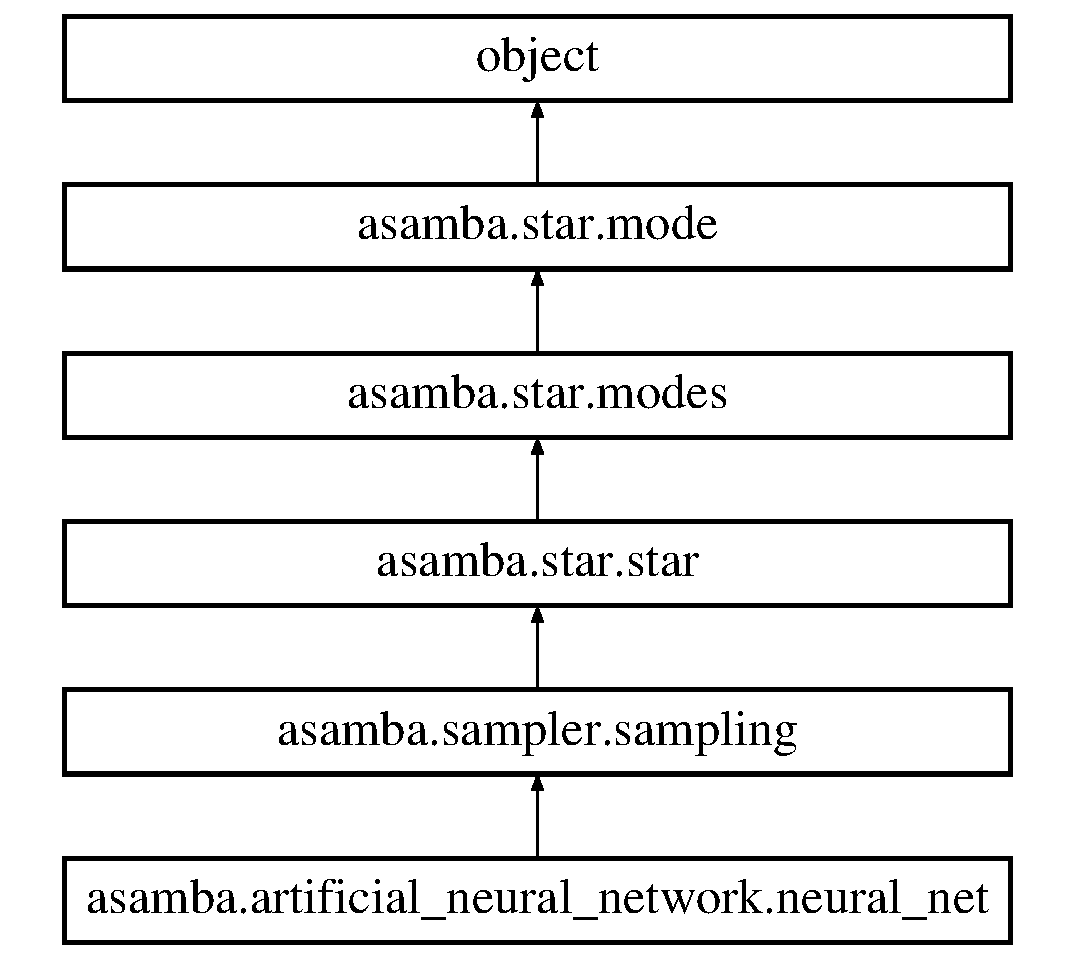
\includegraphics[height=6.000000cm]{classasamba_1_1artificial__neural__network_1_1neural__net}
\end{center}
\end{figure}
\subsection*{Public Member Functions}
\begin{DoxyCompactItemize}
\item 
\mbox{\Hypertarget{classasamba_1_1artificial__neural__network_1_1neural__net_ab35d35b79c522dd0f1e5bf88164e82f3}\label{classasamba_1_1artificial__neural__network_1_1neural__net_ab35d35b79c522dd0f1e5bf88164e82f3}} 
def {\bfseries \+\_\+\+\_\+init\+\_\+\+\_\+} (self)
\item 
\mbox{\Hypertarget{classasamba_1_1artificial__neural__network_1_1neural__net_afb2a64a48856eb07e4f48a3645d30843}\label{classasamba_1_1artificial__neural__network_1_1neural__net_afb2a64a48856eb07e4f48a3645d30843}} 
def \hyperlink{classasamba_1_1artificial__neural__network_1_1neural__net_afb2a64a48856eb07e4f48a3645d30843}{set} (self, attr, val)
\begin{DoxyCompactList}\small\item\em Setter. \end{DoxyCompactList}\item 
\mbox{\Hypertarget{classasamba_1_1artificial__neural__network_1_1neural__net_ad916fe73e8028f451fadbdb0436da70e}\label{classasamba_1_1artificial__neural__network_1_1neural__net_ad916fe73e8028f451fadbdb0436da70e}} 
def \hyperlink{classasamba_1_1artificial__neural__network_1_1neural__net_ad916fe73e8028f451fadbdb0436da70e}{get} (self, attr)
\begin{DoxyCompactList}\small\item\em Getter. \end{DoxyCompactList}\item 
def \hyperlink{classasamba_1_1artificial__neural__network_1_1neural__net_a623b5424543944cb88d5a3a8889e6bbe}{solve\+\_\+normal\+\_\+equation} (self)
\begin{DoxyCompactList}\small\item\em Methods. \end{DoxyCompactList}\item 
def \hyperlink{classasamba_1_1artificial__neural__network_1_1neural__net_ac976779fd464470353ebe1f247314b8a}{chi\+\_\+square} (self)
\item 
def \hyperlink{classasamba_1_1artificial__neural__network_1_1neural__net_a333856c597f409a2ef20e07545baadf1}{max\+\_\+a\+\_\+posteriori} (self)
\item 
def \hyperlink{classasamba_1_1artificial__neural__network_1_1neural__net_a6c9272cb29ab3220ad19ffd3d35495a7}{marginalize\+\_\+wrt} (self, wrt)
\item 
def \hyperlink{classasamba_1_1artificial__neural__network_1_1neural__net_aa5832df25488526021198613fc2f6ce6}{marginalize} (self)
\end{DoxyCompactItemize}
\subsection*{Public Attributes}
\begin{DoxyCompactItemize}
\item 
\mbox{\Hypertarget{classasamba_1_1artificial__neural__network_1_1neural__net_a4ab09b5b637dc7f53b8d59a93b6474e4}\label{classasamba_1_1artificial__neural__network_1_1neural__net_a4ab09b5b637dc7f53b8d59a93b6474e4}} 
{\bfseries normal\+\_\+equation\+\_\+done}
\item 
\mbox{\Hypertarget{classasamba_1_1artificial__neural__network_1_1neural__net_acf888280ab4e318d98f30b198b8ead00}\label{classasamba_1_1artificial__neural__network_1_1neural__net_acf888280ab4e318d98f30b198b8ead00}} 
{\bfseries normal\+\_\+equation\+\_\+theta}
\item 
\mbox{\Hypertarget{classasamba_1_1artificial__neural__network_1_1neural__net_adc2fd98d21454d4d84385cf081b6193e}\label{classasamba_1_1artificial__neural__network_1_1neural__net_adc2fd98d21454d4d84385cf081b6193e}} 
{\bfseries normal\+\_\+equation\+\_\+features}
\item 
\mbox{\Hypertarget{classasamba_1_1artificial__neural__network_1_1neural__net_a57fa03f2b417cbfcc070544ae999a4fa}\label{classasamba_1_1artificial__neural__network_1_1neural__net_a57fa03f2b417cbfcc070544ae999a4fa}} 
{\bfseries normal\+\_\+equation\+\_\+cost}
\item 
\mbox{\Hypertarget{classasamba_1_1artificial__neural__network_1_1neural__net_a99482343ab6e14f2b2299d06f9502c4b}\label{classasamba_1_1artificial__neural__network_1_1neural__net_a99482343ab6e14f2b2299d06f9502c4b}} 
{\bfseries M\+A\+P\+\_\+uniform\+\_\+prior}
\item 
\mbox{\Hypertarget{classasamba_1_1artificial__neural__network_1_1neural__net_a73abc1d438d9caffe5fe1535add5013c}\label{classasamba_1_1artificial__neural__network_1_1neural__net_a73abc1d438d9caffe5fe1535add5013c}} 
{\bfseries M\+A\+P\+\_\+use\+\_\+log\+\_\+\+Teff\+\_\+log\+\_\+g\+\_\+prior}
\item 
\mbox{\Hypertarget{classasamba_1_1artificial__neural__network_1_1neural__net_af486639662cc9a0a09eefa44e3bace5f}\label{classasamba_1_1artificial__neural__network_1_1neural__net_af486639662cc9a0a09eefa44e3bace5f}} 
{\bfseries M\+A\+P\+\_\+prior}
\item 
\mbox{\Hypertarget{classasamba_1_1artificial__neural__network_1_1neural__net_a44e49b7e1b7c6d23d28e19f2fbabe67c}\label{classasamba_1_1artificial__neural__network_1_1neural__net_a44e49b7e1b7c6d23d28e19f2fbabe67c}} 
{\bfseries M\+A\+P\+\_\+ln\+\_\+prior}
\item 
\mbox{\Hypertarget{classasamba_1_1artificial__neural__network_1_1neural__net_ae4b6ad0fb8f1539a45379805604bf091}\label{classasamba_1_1artificial__neural__network_1_1neural__net_ae4b6ad0fb8f1539a45379805604bf091}} 
{\bfseries chi\+\_\+square\+\_\+done}
\item 
\mbox{\Hypertarget{classasamba_1_1artificial__neural__network_1_1neural__net_ac73fdf3dfb1500a70ccfa3a62d279f30}\label{classasamba_1_1artificial__neural__network_1_1neural__net_ac73fdf3dfb1500a70ccfa3a62d279f30}} 
{\bfseries frequency\+\_\+sigma\+\_\+factor}
\item 
\mbox{\Hypertarget{classasamba_1_1artificial__neural__network_1_1neural__net_a9e249497ea1f7700c74ce4e53132ab89}\label{classasamba_1_1artificial__neural__network_1_1neural__net_a9e249497ea1f7700c74ce4e53132ab89}} 
{\bfseries M\+A\+P\+\_\+chi\+\_\+square\+\_\+matrix}
\item 
\mbox{\Hypertarget{classasamba_1_1artificial__neural__network_1_1neural__net_a31d8ee3e87c6844d6dbabf13bdd917fe}\label{classasamba_1_1artificial__neural__network_1_1neural__net_a31d8ee3e87c6844d6dbabf13bdd917fe}} 
{\bfseries M\+A\+P\+\_\+chi\+\_\+square}
\item 
\mbox{\Hypertarget{classasamba_1_1artificial__neural__network_1_1neural__net_ab2950ada903f70215bf38d38a5f34eb3}\label{classasamba_1_1artificial__neural__network_1_1neural__net_ab2950ada903f70215bf38d38a5f34eb3}} 
{\bfseries M\+A\+P\+\_\+likelihood}
\item 
\mbox{\Hypertarget{classasamba_1_1artificial__neural__network_1_1neural__net_a41b9deec89d13536b875662528a72d69}\label{classasamba_1_1artificial__neural__network_1_1neural__net_a41b9deec89d13536b875662528a72d69}} 
{\bfseries M\+A\+P\+\_\+ln\+\_\+likelihood}
\item 
\mbox{\Hypertarget{classasamba_1_1artificial__neural__network_1_1neural__net_afb36d0c0e233608eb9a4433eadbdd789}\label{classasamba_1_1artificial__neural__network_1_1neural__net_afb36d0c0e233608eb9a4433eadbdd789}} 
{\bfseries rescale\+\_\+ln\+\_\+likelihood}
\item 
\mbox{\Hypertarget{classasamba_1_1artificial__neural__network_1_1neural__net_a10e72597954ac3c1bf07776f630bf2c2}\label{classasamba_1_1artificial__neural__network_1_1neural__net_a10e72597954ac3c1bf07776f630bf2c2}} 
{\bfseries M\+A\+P\+\_\+evidence}
\item 
\mbox{\Hypertarget{classasamba_1_1artificial__neural__network_1_1neural__net_aaf8bff278ba4b75f89f288b3d91815d0}\label{classasamba_1_1artificial__neural__network_1_1neural__net_aaf8bff278ba4b75f89f288b3d91815d0}} 
{\bfseries M\+A\+P\+\_\+ln\+\_\+evidence}
\item 
\mbox{\Hypertarget{classasamba_1_1artificial__neural__network_1_1neural__net_ab9d760e895c2e9819cdd8f6293aa057e}\label{classasamba_1_1artificial__neural__network_1_1neural__net_ab9d760e895c2e9819cdd8f6293aa057e}} 
{\bfseries M\+A\+P\+\_\+posterior}
\item 
\mbox{\Hypertarget{classasamba_1_1artificial__neural__network_1_1neural__net_a5932ac64322c8efaa69c9d8295743344}\label{classasamba_1_1artificial__neural__network_1_1neural__net_a5932ac64322c8efaa69c9d8295743344}} 
{\bfseries M\+A\+P\+\_\+ln\+\_\+posterior}
\item 
\mbox{\Hypertarget{classasamba_1_1artificial__neural__network_1_1neural__net_ad9528902cdfd730e5d825e6d3868affc}\label{classasamba_1_1artificial__neural__network_1_1neural__net_ad9528902cdfd730e5d825e6d3868affc}} 
{\bfseries M\+A\+P\+\_\+feature}
\item 
\mbox{\Hypertarget{classasamba_1_1artificial__neural__network_1_1neural__net_af7f78c03187ed9359531a55b7a52008e}\label{classasamba_1_1artificial__neural__network_1_1neural__net_af7f78c03187ed9359531a55b7a52008e}} 
{\bfseries M\+A\+P\+\_\+frequencies}
\item 
\mbox{\Hypertarget{classasamba_1_1artificial__neural__network_1_1neural__net_a3ae7716eb30c21b8b30aaaed771a5e3a}\label{classasamba_1_1artificial__neural__network_1_1neural__net_a3ae7716eb30c21b8b30aaaed771a5e3a}} 
{\bfseries M\+A\+P\+\_\+id\+\_\+track}
\item 
\mbox{\Hypertarget{classasamba_1_1artificial__neural__network_1_1neural__net_a8969c4634111100eea1539b7b11ae31c}\label{classasamba_1_1artificial__neural__network_1_1neural__net_a8969c4634111100eea1539b7b11ae31c}} 
{\bfseries M\+A\+P\+\_\+id\+\_\+model}
\item 
\mbox{\Hypertarget{classasamba_1_1artificial__neural__network_1_1neural__net_a0d9cacebc57b4f5f3011030f5d5aa721}\label{classasamba_1_1artificial__neural__network_1_1neural__net_a0d9cacebc57b4f5f3011030f5d5aa721}} 
{\bfseries M\+A\+P\+\_\+radial\+\_\+orders}
\item 
\mbox{\Hypertarget{classasamba_1_1artificial__neural__network_1_1neural__net_a6fb72c4f6177f96d67bdaa9759b55a6a}\label{classasamba_1_1artificial__neural__network_1_1neural__net_a6fb72c4f6177f96d67bdaa9759b55a6a}} 
{\bfseries M\+A\+P\+\_\+mode\+\_\+types}
\item 
\mbox{\Hypertarget{classasamba_1_1artificial__neural__network_1_1neural__net_a61c3c718b9655a5b3e91c0d2db796351}\label{classasamba_1_1artificial__neural__network_1_1neural__net_a61c3c718b9655a5b3e91c0d2db796351}} 
{\bfseries marginal\+\_\+results}
\item 
\mbox{\Hypertarget{classasamba_1_1artificial__neural__network_1_1neural__net_afc25832fb20e8fdb4064ec38f4d6de70}\label{classasamba_1_1artificial__neural__network_1_1neural__net_afc25832fb20e8fdb4064ec38f4d6de70}} 
{\bfseries marginal\+\_\+features}
\end{DoxyCompactItemize}


\subsection{Detailed Description}
\paragraph*{}

\subsection*{}

\subsection*{}

\subsection*{}

\subsection*{}

\subsection*{}

\subparagraph*{}

\begin{DoxyVerb}\end{DoxyVerb}
 

Definition at line 36 of file artificial\+\_\+neural\+\_\+network.\+py.



\subsection{Member Function Documentation}
\mbox{\Hypertarget{classasamba_1_1artificial__neural__network_1_1neural__net_ac976779fd464470353ebe1f247314b8a}\label{classasamba_1_1artificial__neural__network_1_1neural__net_ac976779fd464470353ebe1f247314b8a}} 
\index{asamba\+::artificial\+\_\+neural\+\_\+network\+::neural\+\_\+net@{asamba\+::artificial\+\_\+neural\+\_\+network\+::neural\+\_\+net}!chi\+\_\+square@{chi\+\_\+square}}
\index{chi\+\_\+square@{chi\+\_\+square}!asamba\+::artificial\+\_\+neural\+\_\+network\+::neural\+\_\+net@{asamba\+::artificial\+\_\+neural\+\_\+network\+::neural\+\_\+net}}
\subsubsection{\texorpdfstring{chi\+\_\+square()}{chi\_square()}}
{\footnotesize\ttfamily def asamba.\+artificial\+\_\+neural\+\_\+network.\+neural\+\_\+net.\+chi\+\_\+square (\begin{DoxyParamCaption}\item[{}]{self }\end{DoxyParamCaption})}

\begin{DoxyVerb}We define the \f$ \chi^2\f$ score between the i-th observed frequency \f$ f_i^{\rm (obs)}, and the model
frequency \f$ f_i^{\rm (mod)}\f$ (coming from e.g. the learning set) as the following

\f[ \chi^2 = \sum_{i=1}^{K} \chi^2_i = \sum_{i=1}^{K} \frac{1}{2}
         \left(\frac{f_i^{\rm (obs) - f_i^{\rm (mod)}{\sigma_i^2}\right)^2. 
\f]

Here, \f$ K\f$ is the total number of observed modes, and \f$\sigma_i\f$ is the 1-\f$\sigma\f$ uncertainty
around each observed frequency.

@param self: An instance of the neural_net() class
@type self: obj
@return: the "MAP_chi_square_matrix" and "MAP_chi_square" attributes of the class will be set
@rtype: None
\end{DoxyVerb}
 

Definition at line 194 of file artificial\+\_\+neural\+\_\+network.\+py.

\mbox{\Hypertarget{classasamba_1_1artificial__neural__network_1_1neural__net_aa5832df25488526021198613fc2f6ce6}\label{classasamba_1_1artificial__neural__network_1_1neural__net_aa5832df25488526021198613fc2f6ce6}} 
\index{asamba\+::artificial\+\_\+neural\+\_\+network\+::neural\+\_\+net@{asamba\+::artificial\+\_\+neural\+\_\+network\+::neural\+\_\+net}!marginalize@{marginalize}}
\index{marginalize@{marginalize}!asamba\+::artificial\+\_\+neural\+\_\+network\+::neural\+\_\+net@{asamba\+::artificial\+\_\+neural\+\_\+network\+::neural\+\_\+net}}
\subsubsection{\texorpdfstring{marginalize()}{marginalize()}}
{\footnotesize\ttfamily def asamba.\+artificial\+\_\+neural\+\_\+network.\+neural\+\_\+net.\+marginalize (\begin{DoxyParamCaption}\item[{}]{self }\end{DoxyParamCaption})}

\begin{DoxyVerb}Iterate over all features in the learning set (whose names are stored in self.sampling.feature_names),
and marginalize with respect to each of these quantities. The outcome of the marginalization will be stored in
two attribute of the neural_net class:

1. marginal_results: which is a list of tuples; read the documentation of marginalize_wrt() method for more info.

2. marginal_features: which is basically cherrypicking of the most likely value from the marginal_features list.
   The order of the outputs here matches exactly that of sampling.features_names

The return structure of "self.marginal_results" is noteworthy. Because we iteratively call the
marginalize_wrt() method and collect its results (tuple with two ndarrays), the "self.marginal_results"
is a list of tuples.
\end{DoxyVerb}
 

Definition at line 266 of file artificial\+\_\+neural\+\_\+network.\+py.

\mbox{\Hypertarget{classasamba_1_1artificial__neural__network_1_1neural__net_a6c9272cb29ab3220ad19ffd3d35495a7}\label{classasamba_1_1artificial__neural__network_1_1neural__net_a6c9272cb29ab3220ad19ffd3d35495a7}} 
\index{asamba\+::artificial\+\_\+neural\+\_\+network\+::neural\+\_\+net@{asamba\+::artificial\+\_\+neural\+\_\+network\+::neural\+\_\+net}!marginalize\+\_\+wrt@{marginalize\+\_\+wrt}}
\index{marginalize\+\_\+wrt@{marginalize\+\_\+wrt}!asamba\+::artificial\+\_\+neural\+\_\+network\+::neural\+\_\+net@{asamba\+::artificial\+\_\+neural\+\_\+network\+::neural\+\_\+net}}
\subsubsection{\texorpdfstring{marginalize\+\_\+wrt()}{marginalize\_wrt()}}
{\footnotesize\ttfamily def asamba.\+artificial\+\_\+neural\+\_\+network.\+neural\+\_\+net.\+marginalize\+\_\+wrt (\begin{DoxyParamCaption}\item[{}]{self,  }\item[{}]{wrt }\end{DoxyParamCaption})}

\begin{DoxyVerb}Marginalize the learning features (learning_x), with respect to (hence "wrt") one of the feature columns (whose names
are available as self.sampling.feature_names)

@param self: an instance of the neural_net() class
@type self: obj
@param wrt: marginalize with respect to
@type wrt: str
@return: a tuple with two members:
 - (ndarray) sorted array of the values of the attribute whose name was passed as wrt, e.g. 'logD'. Note that
   the values in this array are unique, and all repetitions are marginalized over
 - (ndarray) the marginalized posterior probability distribution associated with each of the values in the
   first element of the tuple
@rtype: tuple
\end{DoxyVerb}
 

Definition at line 247 of file artificial\+\_\+neural\+\_\+network.\+py.

\mbox{\Hypertarget{classasamba_1_1artificial__neural__network_1_1neural__net_a333856c597f409a2ef20e07545baadf1}\label{classasamba_1_1artificial__neural__network_1_1neural__net_a333856c597f409a2ef20e07545baadf1}} 
\index{asamba\+::artificial\+\_\+neural\+\_\+network\+::neural\+\_\+net@{asamba\+::artificial\+\_\+neural\+\_\+network\+::neural\+\_\+net}!max\+\_\+a\+\_\+posteriori@{max\+\_\+a\+\_\+posteriori}}
\index{max\+\_\+a\+\_\+posteriori@{max\+\_\+a\+\_\+posteriori}!asamba\+::artificial\+\_\+neural\+\_\+network\+::neural\+\_\+net@{asamba\+::artificial\+\_\+neural\+\_\+network\+::neural\+\_\+net}}
\subsubsection{\texorpdfstring{max\+\_\+a\+\_\+posteriori()}{max\_a\_posteriori()}}
{\footnotesize\ttfamily def asamba.\+artificial\+\_\+neural\+\_\+network.\+neural\+\_\+net.\+max\+\_\+a\+\_\+posteriori (\begin{DoxyParamCaption}\item[{}]{self }\end{DoxyParamCaption})}

\begin{DoxyVerb}This routine finds the attributes of the model which maximizes the posterior likelihood function, hence MAP. 
It consists of the following steps:

1. Priors: Either set uniformly, or are set based on a comparison between log_Teff and log_g of the model and
   the star. For each hypothesis \f$h\f$, we return the prior information \f$P(h)\f$, and \f$\ln P(h)\f$.

2. LogLikelihood, or chi square \f$\chi^2\f$: the natural logarithm of the probability density of the data 
   given the hypothesis, i.e. 
   \f$\chi^2=\ln P(D|h) = \frac{1}{2K}\sum_{i=1}^{K} \left((f_i^{\rm (obs)} - f_i^{\rm (mod)})/sigma_i \right)^2 \f$.
   A recommended option here is to "rescale" the chi-square values to avoid numerical overflow.

3. Evidence, which is basically an inner dot product between the prior vector and the likelihood vector:
   \f$P(D)=\sum_h P(D\h) P(h) \f$. We return both \f$P(D)\f$ and \f$\ln P(D)\f$.

4. Posterior \f$P(h|D)\f$: Based on the Bayes Theorem, the posterior is 

   \f[
   \frac{P(h|D)}{s}=\frac{\frac{P(D|h)}{s}P(h)}{P(D)},
   \f]

   where \f$s\f$ is an optional "scaling" factor used to "rescale" the loglikelihood. Indeed, setting \f$s=1\f$
   recovers the Bayes theorem in its original form. This scaling is allowed, since we only make relative 
   comparison between the models.

@param self: an instance of the neural_net() class    
@type self: obj
\end{DoxyVerb}
 

Definition at line 215 of file artificial\+\_\+neural\+\_\+network.\+py.

\mbox{\Hypertarget{classasamba_1_1artificial__neural__network_1_1neural__net_a623b5424543944cb88d5a3a8889e6bbe}\label{classasamba_1_1artificial__neural__network_1_1neural__net_a623b5424543944cb88d5a3a8889e6bbe}} 
\index{asamba\+::artificial\+\_\+neural\+\_\+network\+::neural\+\_\+net@{asamba\+::artificial\+\_\+neural\+\_\+network\+::neural\+\_\+net}!solve\+\_\+normal\+\_\+equation@{solve\+\_\+normal\+\_\+equation}}
\index{solve\+\_\+normal\+\_\+equation@{solve\+\_\+normal\+\_\+equation}!asamba\+::artificial\+\_\+neural\+\_\+network\+::neural\+\_\+net@{asamba\+::artificial\+\_\+neural\+\_\+network\+::neural\+\_\+net}}
\subsubsection{\texorpdfstring{solve\+\_\+normal\+\_\+equation()}{solve\_normal\_equation()}}
{\footnotesize\ttfamily def asamba.\+artificial\+\_\+neural\+\_\+network.\+neural\+\_\+net.\+solve\+\_\+normal\+\_\+equation (\begin{DoxyParamCaption}\item[{}]{self }\end{DoxyParamCaption})}



Methods. 

\begin{DoxyVerb}Find the analytic solution for the unknown hypothesis coefficients \f$\theta\f$, which minimizes the
cost function \f$ J(\theta) \f$ as defined below.

\f[ J(\theta)= \frac{1}{2m} (\theta^T X-y)^T \cdot (\theta^T X-y) \f]

For more information refer to: 
<a href="http://eli.thegreenplace.net/2014/derivation-of-the-normal-equation-for-linear-regression">Click to Open</a> 
Consequently, the analytic solution to \f$\theta\f$ is:

\f[ \theta_0 = (X^T \cdot X)^{-1} \cdot X^{-1} \cdot y. \f]

A brief remark on the dimensionality of the terms: For a learning set of size \f$ m\f$, with \f$ n+1\f$ features
(including the intercept coefficient), and for the observed/trained output \f$ y \f$ being a matrix of \f$ m\times K\f$
(for \f$ K\f$ modes), then the coefficient matrix \f$ \theta_0\f$ is \f$ (n+1) \times K \f$.

Once \f$\theta_0\f$ is analytically derived, then the cost function is minimized. If we assume
this set of coefficients make the cost function approach zero \f$J(\theta_0)\approx 0\f$, intuitively 
\f$ \theta_0^T\cdot X \approx y \f$. 

One can immediately solve for the unknown feature vector \f$ X \f$, which reproduces the observations \f$ y_0\f$, 
given the corresponding coefficients \f$ \theta_0 \f$. To that end, we multiply both sides of the last equation 
by \f$ \theta \f$, followed by a multiplication with \f$ (\theta_0 \cdot \theta_0^T)^{-1} \f$ to yield \f$ X \f$:

\f[ X_0 \approx (\theta_0 \cdot \theta_0^T)^{-1} \cdot (\theta \cdot y_0) \f]

Needless to highlight that \f$X_0\f$ is a vector of size \f$(n+1)\f$, for an intercept and \f n\f$ features.

Notes:
- The resulting coefficients are saved as the following attribute self.normal_equation_theta, and the resulting
  feature vector \f$ X_0 \f$ is stored as the attribute self.normal_equation_features.
- The model frequencies \f$ y \f$ and the observed frequencies \f$ y_0 \f$ are converted to the per day 
  (\f$ d^{-1} \f$) unit for a fair comparison.
- "A major drawback of the Maximum Likelihood approach is that it is vulnerable to overfitting, because no care
   is taken for cmplex models that try to learn the specificities of the particular training set (Theodoridis, S.
   2015, Machine Learning book)."

@param self: instance of the neural_net class
@type self: object
\end{DoxyVerb}
 

Definition at line 149 of file artificial\+\_\+neural\+\_\+network.\+py.



The documentation for this class was generated from the following file\+:\begin{DoxyCompactItemize}
\item 
artificial\+\_\+neural\+\_\+network.\+py\end{DoxyCompactItemize}

\hypertarget{classasamba_1_1sampler_1_1sampling}{}\section{asamba.\+sampler.\+sampling Class Reference}
\label{classasamba_1_1sampler_1_1sampling}\index{asamba.\+sampler.\+sampling@{asamba.\+sampler.\+sampling}}


\paragraph*{}

\subsection*{}

\subsection*{}

\subsection*{}

\subsection*{}

\subsection*{}

\subparagraph*{} 


Inheritance diagram for asamba.\+sampler.\+sampling\+:\begin{figure}[H]
\begin{center}
\leavevmode
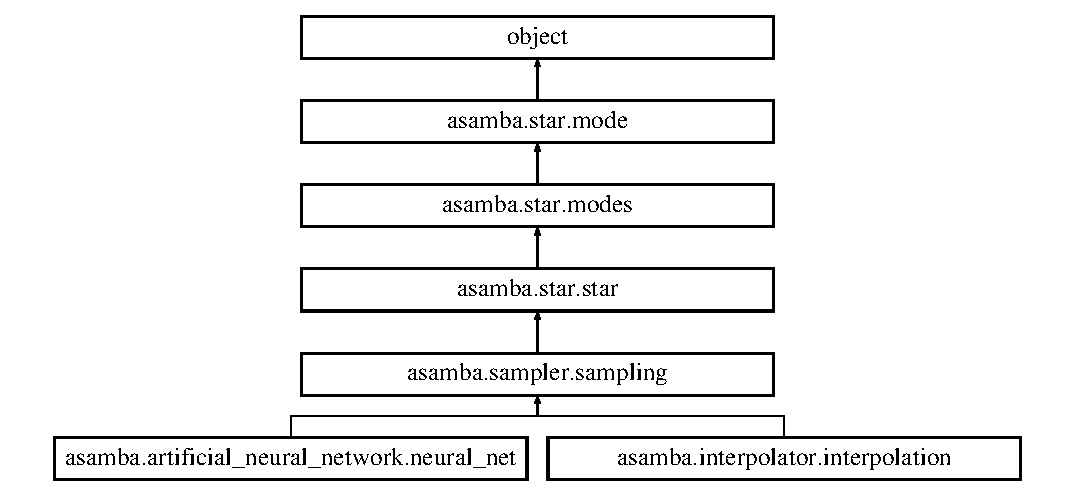
\includegraphics[height=6.000000cm]{classasamba_1_1sampler_1_1sampling}
\end{center}
\end{figure}
\subsection*{Public Member Functions}
\begin{DoxyCompactItemize}
\item 
\mbox{\Hypertarget{classasamba_1_1sampler_1_1sampling_a2551ddd4207eefb6dd3eb669ca92cc3e}\label{classasamba_1_1sampler_1_1sampling_a2551ddd4207eefb6dd3eb669ca92cc3e}} 
def {\bfseries \+\_\+\+\_\+init\+\_\+\+\_\+} (self)
\item 
def \hyperlink{classasamba_1_1sampler_1_1sampling_a682af8a360751e2fb6dd215fe571ea43}{set} (self, attr, val)
\begin{DoxyCompactList}\small\item\em Setter. \end{DoxyCompactList}\item 
def \hyperlink{classasamba_1_1sampler_1_1sampling_a55ebddb5056b66524d34341cccae5d05}{load\+\_\+sampling\+\_\+from\+\_\+inlist} (self, filename)
\item 
def \hyperlink{classasamba_1_1sampler_1_1sampling_a9e11f6bf4371b3dbe372dcc75c47ad3a}{get} (self, attr)
\begin{DoxyCompactList}\small\item\em Getter. \end{DoxyCompactList}\item 
def \hyperlink{classasamba_1_1sampler_1_1sampling_abb689acce45526b082697abe45e2cb56}{build\+\_\+learning\+\_\+set} (self)
\begin{DoxyCompactList}\small\item\em Methods. \end{DoxyCompactList}\item 
def \hyperlink{classasamba_1_1sampler_1_1sampling_ae9c349cf7e5114f9675f07e5b97ed628}{learning\+\_\+log\+\_\+\+Teff\+\_\+log\+\_\+g} (self)
\item 
def \hyperlink{classasamba_1_1sampler_1_1sampling_ae0e3548d71adf58b309904e65b0e6e8c}{split\+\_\+learning\+\_\+sets} (self)
\item 
def \hyperlink{classasamba_1_1sampler_1_1sampling_a64ed2afa6e77447a36512136da5b500a}{get\+\_\+\+M\+\_\+ini\+\_\+fov\+\_\+\+Z\+\_\+log\+D\+\_\+\+Xc\+\_\+from\+\_\+models\+\_\+id} (self, list\+\_\+ids\+\_\+models)
\item 
def \hyperlink{classasamba_1_1sampler_1_1sampling_abdedb54b26dfc7605977d2103ce050b0}{extract\+\_\+gyre\+\_\+modes\+\_\+from\+\_\+id\+\_\+model\+\_\+id\+\_\+rot} (self, list\+\_\+ids\+\_\+models, list\+\_\+ids\+\_\+rot, list\+\_\+rows)
\item 
def \hyperlink{classasamba_1_1sampler_1_1sampling_a75e186291813796d1114ccf2e1f3b2c3}{trim\+\_\+closest\+\_\+modes} (modes, rec\+\_\+gyre, dic\+\_\+mode\+\_\+types, trim\+\_\+delta\+\_\+freq\+\_\+factor)
\begin{DoxyCompactList}\small\item\em Trimming Functions Note\+: The signatures of the following three functions must be identical, because they are tossed into self.\+search\+\_\+function, and can be called from external (inherited) modules. \end{DoxyCompactList}\item 
def \hyperlink{classasamba_1_1sampler_1_1sampling_a8058c0e4f2aa8642f7b19daeb016d73a}{trim\+\_\+modes\+\_\+by\+\_\+dP} (modes, rec\+\_\+gyre, dic\+\_\+mode\+\_\+types, trim\+\_\+delta\+\_\+freq\+\_\+factor)
\item 
def \hyperlink{classasamba_1_1sampler_1_1sampling_a0fe5ca163f5e1c07a017783818535579}{trim\+\_\+modes\+\_\+by\+\_\+df} (modes, rec\+\_\+gyre, dic\+\_\+mode\+\_\+types, trim\+\_\+delta\+\_\+freq\+\_\+factor)
\item 
def \hyperlink{classasamba_1_1sampler_1_1sampling_ad67c8918488194428f7733918a55a4a0}{trim\+\_\+modes} (self, rec\+\_\+gyre, dic\+\_\+mode\+\_\+types)
\end{DoxyCompactItemize}
\subsection*{Public Attributes}
\begin{DoxyCompactItemize}
\item 
\mbox{\Hypertarget{classasamba_1_1sampler_1_1sampling_ae3c9b14c6e2b7ed0e8b14349fca6ed33}\label{classasamba_1_1sampler_1_1sampling_ae3c9b14c6e2b7ed0e8b14349fca6ed33}} 
{\bfseries dbname}
\item 
\mbox{\Hypertarget{classasamba_1_1sampler_1_1sampling_a589acc5a8396b9f00f8d26851e4bc017}\label{classasamba_1_1sampler_1_1sampling_a589acc5a8396b9f00f8d26851e4bc017}} 
{\bfseries use\+\_\+constrained\+\_\+sampling}
\item 
\mbox{\Hypertarget{classasamba_1_1sampler_1_1sampling_a0abd60f79c46e2c855fe6f7a1f8469c4}\label{classasamba_1_1sampler_1_1sampling_a0abd60f79c46e2c855fe6f7a1f8469c4}} 
{\bfseries use\+\_\+random\+\_\+sampling}
\item 
\mbox{\Hypertarget{classasamba_1_1sampler_1_1sampling_a5fa5105e4e10525cc821a279f6e9130c}\label{classasamba_1_1sampler_1_1sampling_a5fa5105e4e10525cc821a279f6e9130c}} 
{\bfseries sampling\+\_\+func\+\_\+name}
\item 
\mbox{\Hypertarget{classasamba_1_1sampler_1_1sampling_a5468f841e18e555e719ea5fe5b2b7501}\label{classasamba_1_1sampler_1_1sampling_a5468f841e18e555e719ea5fe5b2b7501}} 
{\bfseries sampling\+\_\+func}
\item 
\mbox{\Hypertarget{classasamba_1_1sampler_1_1sampling_a5da6b0bcf8404f27f713e4fccec22068}\label{classasamba_1_1sampler_1_1sampling_a5da6b0bcf8404f27f713e4fccec22068}} 
{\bfseries sampling\+\_\+shuffle}
\item 
\mbox{\Hypertarget{classasamba_1_1sampler_1_1sampling_a5d94a7ed123b396c965b1a0895d8e6f4}\label{classasamba_1_1sampler_1_1sampling_a5d94a7ed123b396c965b1a0895d8e6f4}} 
{\bfseries max\+\_\+sample\+\_\+size}
\item 
\mbox{\Hypertarget{classasamba_1_1sampler_1_1sampling_aa88018692ca34106856a89f984d7d52e}\label{classasamba_1_1sampler_1_1sampling_aa88018692ca34106856a89f984d7d52e}} 
{\bfseries range\+\_\+log\+\_\+\+Teff}
\item 
\mbox{\Hypertarget{classasamba_1_1sampler_1_1sampling_a74bdc509d834e5a345b37d4584108262}\label{classasamba_1_1sampler_1_1sampling_a74bdc509d834e5a345b37d4584108262}} 
{\bfseries range\+\_\+log\+\_\+g}
\item 
\mbox{\Hypertarget{classasamba_1_1sampler_1_1sampling_ad40d773c803564dbc19a95288b73ed7c}\label{classasamba_1_1sampler_1_1sampling_ad40d773c803564dbc19a95288b73ed7c}} 
{\bfseries range\+\_\+eta}
\item 
\mbox{\Hypertarget{classasamba_1_1sampler_1_1sampling_ac55cf20b249cb039e6049ea750578b6b}\label{classasamba_1_1sampler_1_1sampling_ac55cf20b249cb039e6049ea750578b6b}} 
{\bfseries ids\+\_\+models}
\item 
\mbox{\Hypertarget{classasamba_1_1sampler_1_1sampling_a9a517de5052801b0e2371fe3967bcdb7}\label{classasamba_1_1sampler_1_1sampling_a9a517de5052801b0e2371fe3967bcdb7}} 
{\bfseries ids\+\_\+rot}
\item 
\mbox{\Hypertarget{classasamba_1_1sampler_1_1sampling_adce94ac7ba9a3ba672ee4ebcd245d026}\label{classasamba_1_1sampler_1_1sampling_adce94ac7ba9a3ba672ee4ebcd245d026}} 
{\bfseries learning\+\_\+done}
\item 
\mbox{\Hypertarget{classasamba_1_1sampler_1_1sampling_ae3cd713dfb67e74e9183c90c81ac9b91}\label{classasamba_1_1sampler_1_1sampling_ae3cd713dfb67e74e9183c90c81ac9b91}} 
{\bfseries exclude\+\_\+eta\+\_\+column}
\item 
\mbox{\Hypertarget{classasamba_1_1sampler_1_1sampling_a9420f2c77fcacb74154b2beb160bcdfe}\label{classasamba_1_1sampler_1_1sampling_a9420f2c77fcacb74154b2beb160bcdfe}} 
{\bfseries num\+\_\+features}
\item 
\mbox{\Hypertarget{classasamba_1_1sampler_1_1sampling_af984009f39bc2e2288c6363e971f434f}\label{classasamba_1_1sampler_1_1sampling_af984009f39bc2e2288c6363e971f434f}} 
{\bfseries feature\+\_\+names}
\item 
\mbox{\Hypertarget{classasamba_1_1sampler_1_1sampling_a6f02b0ed44f4d6129e3be661bc2b3a70}\label{classasamba_1_1sampler_1_1sampling_a6f02b0ed44f4d6129e3be661bc2b3a70}} 
{\bfseries learning\+\_\+ids\+\_\+models}
\item 
\mbox{\Hypertarget{classasamba_1_1sampler_1_1sampling_a2926aa1563a998de742ff085831523ef}\label{classasamba_1_1sampler_1_1sampling_a2926aa1563a998de742ff085831523ef}} 
{\bfseries learning\+\_\+ids\+\_\+rot}
\item 
\mbox{\Hypertarget{classasamba_1_1sampler_1_1sampling_a29c34146d0ae287bfbc2e3967fad4e34}\label{classasamba_1_1sampler_1_1sampling_a29c34146d0ae287bfbc2e3967fad4e34}} 
{\bfseries learning\+\_\+x}
\item 
\mbox{\Hypertarget{classasamba_1_1sampler_1_1sampling_ad29cdc91b7bfae6a00e6d39b1f58f238}\label{classasamba_1_1sampler_1_1sampling_ad29cdc91b7bfae6a00e6d39b1f58f238}} 
{\bfseries learning\+\_\+y}
\item 
\mbox{\Hypertarget{classasamba_1_1sampler_1_1sampling_af7bb28a5bd990445d2eae1a241528bf8}\label{classasamba_1_1sampler_1_1sampling_af7bb28a5bd990445d2eae1a241528bf8}} 
{\bfseries sample\+\_\+size}
\item 
\mbox{\Hypertarget{classasamba_1_1sampler_1_1sampling_a39908bdd8a3b9a314cb2b75e7dc546ed}\label{classasamba_1_1sampler_1_1sampling_a39908bdd8a3b9a314cb2b75e7dc546ed}} 
{\bfseries learning\+\_\+log\+\_\+\+Teff}
\item 
\mbox{\Hypertarget{classasamba_1_1sampler_1_1sampling_a213d8e0aa722b14e348fad4e3dbf5b72}\label{classasamba_1_1sampler_1_1sampling_a213d8e0aa722b14e348fad4e3dbf5b72}} 
{\bfseries learning\+\_\+log\+\_\+g}
\item 
\mbox{\Hypertarget{classasamba_1_1sampler_1_1sampling_aebb4ebee9d878c432168f6ef87c680cf}\label{classasamba_1_1sampler_1_1sampling_aebb4ebee9d878c432168f6ef87c680cf}} 
{\bfseries learning\+\_\+radial\+\_\+orders}
\item 
\mbox{\Hypertarget{classasamba_1_1sampler_1_1sampling_ad0f1cc678b190fa1472e58880f4975f5}\label{classasamba_1_1sampler_1_1sampling_ad0f1cc678b190fa1472e58880f4975f5}} 
{\bfseries learning\+\_\+mode\+\_\+types}
\item 
\mbox{\Hypertarget{classasamba_1_1sampler_1_1sampling_a993e780e274a85a8a397b69e5e054dcc}\label{classasamba_1_1sampler_1_1sampling_a993e780e274a85a8a397b69e5e054dcc}} 
{\bfseries modes\+\_\+id\+\_\+types}
\item 
\mbox{\Hypertarget{classasamba_1_1sampler_1_1sampling_a61d875d585ecfa4932291af6b26a9843}\label{classasamba_1_1sampler_1_1sampling_a61d875d585ecfa4932291af6b26a9843}} 
{\bfseries modes\+\_\+freq\+\_\+range}
\item 
\mbox{\Hypertarget{classasamba_1_1sampler_1_1sampling_ad3791306712fccfd8c1b92e89929165e}\label{classasamba_1_1sampler_1_1sampling_ad3791306712fccfd8c1b92e89929165e}} 
{\bfseries search\+\_\+function}
\item 
\mbox{\Hypertarget{classasamba_1_1sampler_1_1sampling_ae388f6d2dd2cdb7ab3a4c06f389c5db8}\label{classasamba_1_1sampler_1_1sampling_ae388f6d2dd2cdb7ab3a4c06f389c5db8}} 
{\bfseries search\+\_\+for\+\_\+closest\+\_\+frequencies}
\item 
\mbox{\Hypertarget{classasamba_1_1sampler_1_1sampling_a1708b7cb7730f4e85b9821cafc534241}\label{classasamba_1_1sampler_1_1sampling_a1708b7cb7730f4e85b9821cafc534241}} 
{\bfseries search\+\_\+strictly\+\_\+for\+\_\+dP}
\item 
\mbox{\Hypertarget{classasamba_1_1sampler_1_1sampling_a2d6b91c616a0de9e0e058d7394c07aa3}\label{classasamba_1_1sampler_1_1sampling_a2d6b91c616a0de9e0e058d7394c07aa3}} 
{\bfseries search\+\_\+strictly\+\_\+for\+\_\+df}
\item 
\mbox{\Hypertarget{classasamba_1_1sampler_1_1sampling_a07a61bc0c96faf223e4e69401ab16e65}\label{classasamba_1_1sampler_1_1sampling_a07a61bc0c96faf223e4e69401ab16e65}} 
{\bfseries match\+\_\+lowest\+\_\+frequency}
\item 
\mbox{\Hypertarget{classasamba_1_1sampler_1_1sampling_ad2eaa097f99e3906f6de7eeaed61feb3}\label{classasamba_1_1sampler_1_1sampling_ad2eaa097f99e3906f6de7eeaed61feb3}} 
{\bfseries trim\+\_\+delta\+\_\+freq\+\_\+factor}
\item 
\mbox{\Hypertarget{classasamba_1_1sampler_1_1sampling_a777fe570dd82981ed9dcf93300a45274}\label{classasamba_1_1sampler_1_1sampling_a777fe570dd82981ed9dcf93300a45274}} 
{\bfseries training\+\_\+percentage}
\item 
\mbox{\Hypertarget{classasamba_1_1sampler_1_1sampling_a56d9a80694ff18be9c3160d7166d265d}\label{classasamba_1_1sampler_1_1sampling_a56d9a80694ff18be9c3160d7166d265d}} 
{\bfseries training\+\_\+size}
\item 
\mbox{\Hypertarget{classasamba_1_1sampler_1_1sampling_a6e3210ceaf457fc63234bb3b880272e5}\label{classasamba_1_1sampler_1_1sampling_a6e3210ceaf457fc63234bb3b880272e5}} 
{\bfseries training\+\_\+x}
\item 
\mbox{\Hypertarget{classasamba_1_1sampler_1_1sampling_ad3e7389fabd7b3d5a7578f31c40c665e}\label{classasamba_1_1sampler_1_1sampling_ad3e7389fabd7b3d5a7578f31c40c665e}} 
{\bfseries training\+\_\+y}
\item 
\mbox{\Hypertarget{classasamba_1_1sampler_1_1sampling_a96ea30c13d9643fc573e00e092518224}\label{classasamba_1_1sampler_1_1sampling_a96ea30c13d9643fc573e00e092518224}} 
{\bfseries training\+\_\+log\+\_\+\+Teff}
\item 
\mbox{\Hypertarget{classasamba_1_1sampler_1_1sampling_a5a18cd0b6f1e94fce04bf498707fce85}\label{classasamba_1_1sampler_1_1sampling_a5a18cd0b6f1e94fce04bf498707fce85}} 
{\bfseries training\+\_\+log\+\_\+g}
\item 
\mbox{\Hypertarget{classasamba_1_1sampler_1_1sampling_a21f67468dd8f4153600b7d91c4b092c4}\label{classasamba_1_1sampler_1_1sampling_a21f67468dd8f4153600b7d91c4b092c4}} 
{\bfseries training\+\_\+set\+\_\+done}
\item 
\mbox{\Hypertarget{classasamba_1_1sampler_1_1sampling_aafc92cfb36fb9e4d2fa186b2d12baead}\label{classasamba_1_1sampler_1_1sampling_aafc92cfb36fb9e4d2fa186b2d12baead}} 
{\bfseries cross\+\_\+valid\+\_\+percentage}
\item 
\mbox{\Hypertarget{classasamba_1_1sampler_1_1sampling_adaa625c45da7ac3f97b45758c5f15268}\label{classasamba_1_1sampler_1_1sampling_adaa625c45da7ac3f97b45758c5f15268}} 
{\bfseries cross\+\_\+valid\+\_\+size}
\item 
\mbox{\Hypertarget{classasamba_1_1sampler_1_1sampling_a8d298377398af0cab3386248ceb95b98}\label{classasamba_1_1sampler_1_1sampling_a8d298377398af0cab3386248ceb95b98}} 
{\bfseries cross\+\_\+valid\+\_\+x}
\item 
\mbox{\Hypertarget{classasamba_1_1sampler_1_1sampling_a7aa489f44c493aba0d74e92656cdfbb7}\label{classasamba_1_1sampler_1_1sampling_a7aa489f44c493aba0d74e92656cdfbb7}} 
{\bfseries cross\+\_\+valid\+\_\+y}
\item 
\mbox{\Hypertarget{classasamba_1_1sampler_1_1sampling_ab5ae6f97f27bbbfc647f737051390b6b}\label{classasamba_1_1sampler_1_1sampling_ab5ae6f97f27bbbfc647f737051390b6b}} 
{\bfseries cross\+\_\+valid\+\_\+log\+\_\+\+Teff}
\item 
\mbox{\Hypertarget{classasamba_1_1sampler_1_1sampling_a885317dc8020e2dca023d5c172ab0378}\label{classasamba_1_1sampler_1_1sampling_a885317dc8020e2dca023d5c172ab0378}} 
{\bfseries cross\+\_\+valid\+\_\+log\+\_\+g}
\item 
\mbox{\Hypertarget{classasamba_1_1sampler_1_1sampling_a2b6fdb6d09da0f3202af2c13db8b031b}\label{classasamba_1_1sampler_1_1sampling_a2b6fdb6d09da0f3202af2c13db8b031b}} 
{\bfseries cross\+\_\+valid\+\_\+set\+\_\+done}
\item 
\mbox{\Hypertarget{classasamba_1_1sampler_1_1sampling_a63b781e64024a63fe80901439b777c32}\label{classasamba_1_1sampler_1_1sampling_a63b781e64024a63fe80901439b777c32}} 
{\bfseries test\+\_\+percentage}
\item 
\mbox{\Hypertarget{classasamba_1_1sampler_1_1sampling_a1233091c7ec9d729334b103cf6d22a13}\label{classasamba_1_1sampler_1_1sampling_a1233091c7ec9d729334b103cf6d22a13}} 
{\bfseries test\+\_\+size}
\item 
\mbox{\Hypertarget{classasamba_1_1sampler_1_1sampling_af5e6dff62618792e7c71d7051475697a}\label{classasamba_1_1sampler_1_1sampling_af5e6dff62618792e7c71d7051475697a}} 
{\bfseries test\+\_\+x}
\item 
\mbox{\Hypertarget{classasamba_1_1sampler_1_1sampling_ae9df70e624b576992754d5c94e7b29a3}\label{classasamba_1_1sampler_1_1sampling_ae9df70e624b576992754d5c94e7b29a3}} 
{\bfseries test\+\_\+y}
\item 
\mbox{\Hypertarget{classasamba_1_1sampler_1_1sampling_ac04c057284530c6b1b1db81efab59d02}\label{classasamba_1_1sampler_1_1sampling_ac04c057284530c6b1b1db81efab59d02}} 
{\bfseries test\+\_\+log\+\_\+\+Teff}
\item 
\mbox{\Hypertarget{classasamba_1_1sampler_1_1sampling_a2d6308328350d4d8e807a76f016f53f9}\label{classasamba_1_1sampler_1_1sampling_a2d6308328350d4d8e807a76f016f53f9}} 
{\bfseries test\+\_\+log\+\_\+g}
\item 
\mbox{\Hypertarget{classasamba_1_1sampler_1_1sampling_a5576728203ff7da70308dd5bf6cedc23}\label{classasamba_1_1sampler_1_1sampling_a5576728203ff7da70308dd5bf6cedc23}} 
{\bfseries test\+\_\+set\+\_\+done}
\end{DoxyCompactItemize}


\subsection{Detailed Description}
\paragraph*{}

\subsection*{}

\subsection*{}

\subsection*{}

\subsection*{}

\subsection*{}

\subparagraph*{}

\begin{DoxyVerb}This class carries out sampling of the learning sets from the database. This class inherits the
"star.star()" object to represent a star
\end{DoxyVerb}
 

Definition at line 45 of file sampler.\+py.



\subsection{Member Function Documentation}
\mbox{\Hypertarget{classasamba_1_1sampler_1_1sampling_abb689acce45526b082697abe45e2cb56}\label{classasamba_1_1sampler_1_1sampling_abb689acce45526b082697abe45e2cb56}} 
\index{asamba\+::sampler\+::sampling@{asamba\+::sampler\+::sampling}!build\+\_\+learning\+\_\+set@{build\+\_\+learning\+\_\+set}}
\index{build\+\_\+learning\+\_\+set@{build\+\_\+learning\+\_\+set}!asamba\+::sampler\+::sampling@{asamba\+::sampler\+::sampling}}
\subsubsection{\texorpdfstring{build\+\_\+learning\+\_\+set()}{build\_learning\_set()}}
{\footnotesize\ttfamily def asamba.\+sampler.\+sampling.\+build\+\_\+learning\+\_\+set (\begin{DoxyParamCaption}\item[{}]{self }\end{DoxyParamCaption})}



Methods. 

\begin{DoxyVerb}This routine prepares a learning (training + cross-validation + test) set from the "tracks", "models",
and "rotation_rates" table from the database "dbname". The sampling method of the data (constrained or
unconstrained) is specified by passing the function name as "sampling_func", with the function arguments
"sampling_args".

The result from this function can be used to randomly build training, cross-validation, and/or test
sets by random slicing.

@param self: An instance of the sampling class
@type self: obj
@return: None. However, the "self.sample" attribute is set to a numpy record array whose columns are
  the following:
  - M_ini: initial mass of the model
  - fov: overshoot free parameter
  - Z: metallicity
  - logD: logarithm of extra diffusive mixing
  - Xc: central hydrogen mass fraction
  - eta: percentage rotation rate w.r.t. to the break up
@rtype: None
\end{DoxyVerb}
 

Definition at line 280 of file sampler.\+py.

\mbox{\Hypertarget{classasamba_1_1sampler_1_1sampling_abdedb54b26dfc7605977d2103ce050b0}\label{classasamba_1_1sampler_1_1sampling_abdedb54b26dfc7605977d2103ce050b0}} 
\index{asamba\+::sampler\+::sampling@{asamba\+::sampler\+::sampling}!extract\+\_\+gyre\+\_\+modes\+\_\+from\+\_\+id\+\_\+model\+\_\+id\+\_\+rot@{extract\+\_\+gyre\+\_\+modes\+\_\+from\+\_\+id\+\_\+model\+\_\+id\+\_\+rot}}
\index{extract\+\_\+gyre\+\_\+modes\+\_\+from\+\_\+id\+\_\+model\+\_\+id\+\_\+rot@{extract\+\_\+gyre\+\_\+modes\+\_\+from\+\_\+id\+\_\+model\+\_\+id\+\_\+rot}!asamba\+::sampler\+::sampling@{asamba\+::sampler\+::sampling}}
\subsubsection{\texorpdfstring{extract\+\_\+gyre\+\_\+modes\+\_\+from\+\_\+id\+\_\+model\+\_\+id\+\_\+rot()}{extract\_gyre\_modes\_from\_id\_model\_id\_rot()}}
{\footnotesize\ttfamily def asamba.\+sampler.\+sampling.\+extract\+\_\+gyre\+\_\+modes\+\_\+from\+\_\+id\+\_\+model\+\_\+id\+\_\+rot (\begin{DoxyParamCaption}\item[{}]{self,  }\item[{}]{list\+\_\+ids\+\_\+models,  }\item[{}]{list\+\_\+ids\+\_\+rot,  }\item[{}]{list\+\_\+rows }\end{DoxyParamCaption})}

\begin{DoxyVerb}This finds a GYRE outputs for a model given its id_model, and id_rot. Then, it slices the
modes based on the observed list, to ensure that there is a "reasonable" match between the
model and observed frequencies. It returns various useful info, only for those models that
survive the frequency filtering.

@param self: an instance of the sampler class
@type self: object
@param list_ids_models: is a list of the id_model for all input models
@type list_ids_models: list
@param list_ids_rot: is a list of the id_rot for all input models
@type list_ids_rot: list
@param list_rows: a list of tuples, where each tuple is e.g. (M_ini, fov, Z, logD, Xc) for
     the input models. 
@tupe list_rows: list
@return: The following items are packed into the returned data structure:
   - list of (M_ini, fov, Z, logD) attribute tuples which fulfil the trimming condition. 
   - list of id_model which fulfil the trimming condition. This is basically
     a subset of the input list.
   - List of id_rot which fulfil the trimming condition. This is basically
     a subset of the input list.
   - List of record arrays for the corresponding models which fulfil the frequency
     filtering criteria.
@rtype: tuple
\end{DoxyVerb}
 

Definition at line 375 of file sampler.\+py.

\mbox{\Hypertarget{classasamba_1_1sampler_1_1sampling_a9e11f6bf4371b3dbe372dcc75c47ad3a}\label{classasamba_1_1sampler_1_1sampling_a9e11f6bf4371b3dbe372dcc75c47ad3a}} 
\index{asamba\+::sampler\+::sampling@{asamba\+::sampler\+::sampling}!get@{get}}
\index{get@{get}!asamba\+::sampler\+::sampling@{asamba\+::sampler\+::sampling}}
\subsubsection{\texorpdfstring{get()}{get()}}
{\footnotesize\ttfamily def asamba.\+sampler.\+sampling.\+get (\begin{DoxyParamCaption}\item[{}]{self,  }\item[{}]{attr }\end{DoxyParamCaption})}



Getter. 

\begin{DoxyVerb}General-purpose method to get the value of a canonical attribute of the object
E.g.

>>>MySample = MyProblem.get('learning_x')

@param attr: the name of the available attribute of the class
@type attr: string
@return: the value of the attribute
@rtype: float
\end{DoxyVerb}
 

Definition at line 257 of file sampler.\+py.

\mbox{\Hypertarget{classasamba_1_1sampler_1_1sampling_a64ed2afa6e77447a36512136da5b500a}\label{classasamba_1_1sampler_1_1sampling_a64ed2afa6e77447a36512136da5b500a}} 
\index{asamba\+::sampler\+::sampling@{asamba\+::sampler\+::sampling}!get\+\_\+\+M\+\_\+ini\+\_\+fov\+\_\+\+Z\+\_\+log\+D\+\_\+\+Xc\+\_\+from\+\_\+models\+\_\+id@{get\+\_\+\+M\+\_\+ini\+\_\+fov\+\_\+\+Z\+\_\+log\+D\+\_\+\+Xc\+\_\+from\+\_\+models\+\_\+id}}
\index{get\+\_\+\+M\+\_\+ini\+\_\+fov\+\_\+\+Z\+\_\+log\+D\+\_\+\+Xc\+\_\+from\+\_\+models\+\_\+id@{get\+\_\+\+M\+\_\+ini\+\_\+fov\+\_\+\+Z\+\_\+log\+D\+\_\+\+Xc\+\_\+from\+\_\+models\+\_\+id}!asamba\+::sampler\+::sampling@{asamba\+::sampler\+::sampling}}
\subsubsection{\texorpdfstring{get\+\_\+\+M\+\_\+ini\+\_\+fov\+\_\+\+Z\+\_\+log\+D\+\_\+\+Xc\+\_\+from\+\_\+models\+\_\+id()}{get\_M\_ini\_fov\_Z\_logD\_Xc\_from\_models\_id()}}
{\footnotesize\ttfamily def asamba.\+sampler.\+sampling.\+get\+\_\+\+M\+\_\+ini\+\_\+fov\+\_\+\+Z\+\_\+log\+D\+\_\+\+Xc\+\_\+from\+\_\+models\+\_\+id (\begin{DoxyParamCaption}\item[{}]{self,  }\item[{}]{list\+\_\+ids\+\_\+models }\end{DoxyParamCaption})}

\begin{DoxyVerb}This routine queries the models table in the database, and returns tuples of the global attributes
(M_ini, fov, Z, logD, Xc) that match the models.id passed by as the "list_ids_models" argument.
This routine can lie in the heart of many applications which require retrieving of the global attributes
by only providing/knowing the corresponding model id.

Note: Even if one model id is passed (repeated) several times in the following query, only the first
occurance is effective. Therefore, the size of the returned results from the following query
is a factor (len(set(ids_rot))) larger than the result of the query. Then, the problem of 1-to-1
matching is resolved by setting up a look-up dictionary, internally.

@param self: an instance of the sampler.sampling class
@type self: object
@param list_ids_models: the list of models.id (integers) giving the exact models.id as in the database
@type list_ids_models: list of integers
@return: tuples of the corresponding attributes/feature values (M_ini, fov, Z, logD, Xc) for the unique
  values in the input list_ids_models. The repeated ids will be reconstructed by walking through the
  input models.id and putting the excluded attributes back in their place.
@rtype: list of tuples
\end{DoxyVerb}
 

Definition at line 351 of file sampler.\+py.

\mbox{\Hypertarget{classasamba_1_1sampler_1_1sampling_ae9c349cf7e5114f9675f07e5b97ed628}\label{classasamba_1_1sampler_1_1sampling_ae9c349cf7e5114f9675f07e5b97ed628}} 
\index{asamba\+::sampler\+::sampling@{asamba\+::sampler\+::sampling}!learning\+\_\+log\+\_\+\+Teff\+\_\+log\+\_\+g@{learning\+\_\+log\+\_\+\+Teff\+\_\+log\+\_\+g}}
\index{learning\+\_\+log\+\_\+\+Teff\+\_\+log\+\_\+g@{learning\+\_\+log\+\_\+\+Teff\+\_\+log\+\_\+g}!asamba\+::sampler\+::sampling@{asamba\+::sampler\+::sampling}}
\subsubsection{\texorpdfstring{learning\+\_\+log\+\_\+\+Teff\+\_\+log\+\_\+g()}{learning\_log\_Teff\_log\_g()}}
{\footnotesize\ttfamily def asamba.\+sampler.\+sampling.\+learning\+\_\+log\+\_\+\+Teff\+\_\+log\+\_\+g (\begin{DoxyParamCaption}\item[{}]{self }\end{DoxyParamCaption})}

\begin{DoxyVerb}Fill up the "models_log_Teff" and "models_log_g" attributes of the class with the corresponding values retrieved
from the models_ids. The resulting arrays are significantly important when dealing with priors for the Bayesian
learning (see, e.g. artificial_neural_network.set_priors() method).
\end{DoxyVerb}
 

Definition at line 306 of file sampler.\+py.

\mbox{\Hypertarget{classasamba_1_1sampler_1_1sampling_a55ebddb5056b66524d34341cccae5d05}\label{classasamba_1_1sampler_1_1sampling_a55ebddb5056b66524d34341cccae5d05}} 
\index{asamba\+::sampler\+::sampling@{asamba\+::sampler\+::sampling}!load\+\_\+sampling\+\_\+from\+\_\+inlist@{load\+\_\+sampling\+\_\+from\+\_\+inlist}}
\index{load\+\_\+sampling\+\_\+from\+\_\+inlist@{load\+\_\+sampling\+\_\+from\+\_\+inlist}!asamba\+::sampler\+::sampling@{asamba\+::sampler\+::sampling}}
\subsubsection{\texorpdfstring{load\+\_\+sampling\+\_\+from\+\_\+inlist()}{load\_sampling\_from\_inlist()}}
{\footnotesize\ttfamily def asamba.\+sampler.\+sampling.\+load\+\_\+sampling\+\_\+from\+\_\+inlist (\begin{DoxyParamCaption}\item[{}]{self,  }\item[{}]{filename }\end{DoxyParamCaption})}

\begin{DoxyVerb}Set some of the attributes of the sampling object through an inlist file. This allows to control
the behaviour of the sampling procedure in an easier way, e.g. through the frontend GUI. For every
valid input variable and its input value, the set method is called iteratively.

@param filename: Full path to the input inlist file. One example can be found in the following 
   directory: <asamba>/data/input_templates/instructions.sampling
@type filename: str
@return: None
\end{DoxyVerb}
 

Definition at line 237 of file sampler.\+py.

\mbox{\Hypertarget{classasamba_1_1sampler_1_1sampling_a682af8a360751e2fb6dd215fe571ea43}\label{classasamba_1_1sampler_1_1sampling_a682af8a360751e2fb6dd215fe571ea43}} 
\index{asamba\+::sampler\+::sampling@{asamba\+::sampler\+::sampling}!set@{set}}
\index{set@{set}!asamba\+::sampler\+::sampling@{asamba\+::sampler\+::sampling}}
\subsubsection{\texorpdfstring{set()}{set()}}
{\footnotesize\ttfamily def asamba.\+sampler.\+sampling.\+set (\begin{DoxyParamCaption}\item[{}]{self,  }\item[{}]{attr,  }\item[{}]{val }\end{DoxyParamCaption})}



Setter. 

\begin{DoxyVerb}Set a sampling attribute, e.g.
>>>MySample = sampler.sampling()
>>>MySample.set('range_log_Teff', [4.12, 4.27])

@param attr: The name of the attribute to set
@type attr: str
@param val: The corresponding data (type and value) for the attribute. 
   Note that the users is mainly responsible for the sanity of the input values, 
   though we internally check for some basic compatibility. The val can take any
   datatype
@type val: int, float, bool, list, etc.
\end{DoxyVerb}
 

Definition at line 181 of file sampler.\+py.

\mbox{\Hypertarget{classasamba_1_1sampler_1_1sampling_ae0e3548d71adf58b309904e65b0e6e8c}\label{classasamba_1_1sampler_1_1sampling_ae0e3548d71adf58b309904e65b0e6e8c}} 
\index{asamba\+::sampler\+::sampling@{asamba\+::sampler\+::sampling}!split\+\_\+learning\+\_\+sets@{split\+\_\+learning\+\_\+sets}}
\index{split\+\_\+learning\+\_\+sets@{split\+\_\+learning\+\_\+sets}!asamba\+::sampler\+::sampling@{asamba\+::sampler\+::sampling}}
\subsubsection{\texorpdfstring{split\+\_\+learning\+\_\+sets()}{split\_learning\_sets()}}
{\footnotesize\ttfamily def asamba.\+sampler.\+sampling.\+split\+\_\+learning\+\_\+sets (\begin{DoxyParamCaption}\item[{}]{self }\end{DoxyParamCaption})}

\begin{DoxyVerb}Split the learning set (prepared by calling build_learning_sets) into a training set, cross-validation
set, and a test set. To do such, the following three attributes of the "sampling" class is used (so, they
must have been already set to their non-default value):
  - training_percentage: (default -1); valid range: 0 to 100
  - cross_valid_percentage: (default -1); valid range: 0 to 100
  - test_percentage: (default -1); valid range: 0 to 100
As a result of applying this method, the following variables are set
  - training_size = -1
  - training_x = -1
  - training_y = -1

  - cross_valid_size = -1
  - cross_valid_x = -1
  - cross_valid_y = -1

  - test_size = -1
  - test_x = -1
  - test_y = -1

Note: once the training/cross-validation/test sets (i.e. *_x and *_y) are prepared, they are randomly
  shuffled internally. So, one shall never reshuffle them, else the ordering of different arrays 
  become inconsistent.

@param self: An instance of the sampling class
@type self: obj
@return: the above nine parameters will be set
@rtype: None
\end{DoxyVerb}
 

Definition at line 315 of file sampler.\+py.

\mbox{\Hypertarget{classasamba_1_1sampler_1_1sampling_a75e186291813796d1114ccf2e1f3b2c3}\label{classasamba_1_1sampler_1_1sampling_a75e186291813796d1114ccf2e1f3b2c3}} 
\index{asamba\+::sampler\+::sampling@{asamba\+::sampler\+::sampling}!trim\+\_\+closest\+\_\+modes@{trim\+\_\+closest\+\_\+modes}}
\index{trim\+\_\+closest\+\_\+modes@{trim\+\_\+closest\+\_\+modes}!asamba\+::sampler\+::sampling@{asamba\+::sampler\+::sampling}}
\subsubsection{\texorpdfstring{trim\+\_\+closest\+\_\+modes()}{trim\_closest\_modes()}}
{\footnotesize\ttfamily def asamba.\+sampler.\+sampling.\+trim\+\_\+closest\+\_\+modes (\begin{DoxyParamCaption}\item[{}]{modes,  }\item[{}]{rec\+\_\+gyre,  }\item[{}]{dic\+\_\+mode\+\_\+types,  }\item[{}]{trim\+\_\+delta\+\_\+freq\+\_\+factor }\end{DoxyParamCaption})}



Trimming Functions Note\+: The signatures of the following three functions must be identical, because they are tossed into self.\+search\+\_\+function, and can be called from external (inherited) modules. 

\begin{DoxyVerb}Not developed yet \end{DoxyVerb}
 

Definition at line 408 of file sampler.\+py.

\mbox{\Hypertarget{classasamba_1_1sampler_1_1sampling_ad67c8918488194428f7733918a55a4a0}\label{classasamba_1_1sampler_1_1sampling_ad67c8918488194428f7733918a55a4a0}} 
\index{asamba\+::sampler\+::sampling@{asamba\+::sampler\+::sampling}!trim\+\_\+modes@{trim\+\_\+modes}}
\index{trim\+\_\+modes@{trim\+\_\+modes}!asamba\+::sampler\+::sampling@{asamba\+::sampler\+::sampling}}
\subsubsection{\texorpdfstring{trim\+\_\+modes()}{trim\_modes()}}
{\footnotesize\ttfamily def asamba.\+sampler.\+sampling.\+trim\+\_\+modes (\begin{DoxyParamCaption}\item[{}]{self,  }\item[{}]{rec\+\_\+gyre,  }\item[{}]{dic\+\_\+mode\+\_\+types }\end{DoxyParamCaption})}

\begin{DoxyVerb}Plan a strategy to trim the GYRE frequency list, and adapt it to the observed list based on the 
requests of the user, i.e. based on the following attributes of the sampling object: 
- search_for_closest_frequencies (Default = False)
- search_strictly_for_dP (Default = False)
- search_strictly_for_df (Default = False)
- match_lowest_frequency (Default = True)
- match_lowest_frequency (Default = 3.0)

Note: The first three booleans specify the search method, and they are all False by defult. We check
internally that only one of the flags is set to True, and the rest being False!

Note: The return value from this routine is identical to the return from the following three functions:
- _trim_closest_modes()
- _trim_modes_by_dP()
- _trim_modes_by_df()

@param self: an instance of the "sampler.sampling" class
@type self: object
@param rec_gyre: the GYRE output list of frequencies as fetched from the database. The following
     columns are available here:
     - id_model: int32
     - id_rot: int16
     - n: int16
     - id_type: int16
     - freq: float32
@type rec_gyre: np.recarray
@param dic_mode_types: Look up dictionary to match the modes identification (l, m) with the modes.id_type
  attribute in the database. This dictionary is fetched from db_lib.get_dic_look_up_mode_types_id(). 
  However, we pass it as an argument instead of fetching it internally to speed up this function.
@type dic_mode_types: dict
@return: False, if for any reason no match is found between the observed and the modeled frequency lists.
     If successful, a matching slice of the input GYRE frequency list is returned.
@rtype: np.recarray or bool
\end{DoxyVerb}
 

Definition at line 445 of file sampler.\+py.

\mbox{\Hypertarget{classasamba_1_1sampler_1_1sampling_a0fe5ca163f5e1c07a017783818535579}\label{classasamba_1_1sampler_1_1sampling_a0fe5ca163f5e1c07a017783818535579}} 
\index{asamba\+::sampler\+::sampling@{asamba\+::sampler\+::sampling}!trim\+\_\+modes\+\_\+by\+\_\+df@{trim\+\_\+modes\+\_\+by\+\_\+df}}
\index{trim\+\_\+modes\+\_\+by\+\_\+df@{trim\+\_\+modes\+\_\+by\+\_\+df}!asamba\+::sampler\+::sampling@{asamba\+::sampler\+::sampling}}
\subsubsection{\texorpdfstring{trim\+\_\+modes\+\_\+by\+\_\+df()}{trim\_modes\_by\_df()}}
{\footnotesize\ttfamily def asamba.\+sampler.\+sampling.\+trim\+\_\+modes\+\_\+by\+\_\+df (\begin{DoxyParamCaption}\item[{}]{modes,  }\item[{}]{rec\+\_\+gyre,  }\item[{}]{dic\+\_\+mode\+\_\+types,  }\item[{}]{trim\+\_\+delta\+\_\+freq\+\_\+factor }\end{DoxyParamCaption})}

\begin{DoxyVerb}Not developed yet \end{DoxyVerb}
 

Definition at line 440 of file sampler.\+py.

\mbox{\Hypertarget{classasamba_1_1sampler_1_1sampling_a8058c0e4f2aa8642f7b19daeb016d73a}\label{classasamba_1_1sampler_1_1sampling_a8058c0e4f2aa8642f7b19daeb016d73a}} 
\index{asamba\+::sampler\+::sampling@{asamba\+::sampler\+::sampling}!trim\+\_\+modes\+\_\+by\+\_\+dP@{trim\+\_\+modes\+\_\+by\+\_\+dP}}
\index{trim\+\_\+modes\+\_\+by\+\_\+dP@{trim\+\_\+modes\+\_\+by\+\_\+dP}!asamba\+::sampler\+::sampling@{asamba\+::sampler\+::sampling}}
\subsubsection{\texorpdfstring{trim\+\_\+modes\+\_\+by\+\_\+d\+P()}{trim\_modes\_by\_dP()}}
{\footnotesize\ttfamily def asamba.\+sampler.\+sampling.\+trim\+\_\+modes\+\_\+by\+\_\+dP (\begin{DoxyParamCaption}\item[{}]{modes,  }\item[{}]{rec\+\_\+gyre,  }\item[{}]{dic\+\_\+mode\+\_\+types,  }\item[{}]{trim\+\_\+delta\+\_\+freq\+\_\+factor }\end{DoxyParamCaption})}

\begin{DoxyVerb}As the name explains, this function receives a record array of GYRE modes summary, and trims/clips
the modes based on their period spacing pattern

@param modes: The observed modes, where each mode in the list is an instance of the "star.mode" class
@type modes: list of star.mode
@param rec_gyre: The numpy record array from GYRE frequency list coming from one GYRE output file
@type rec_gyre: np.recarray
@param dic_mode_types: Look up dictionary to match the modes identification (l, m) with the modes.id_type
  attribute in the database. This dictionary is fetched from db_lib.get_dic_look_up_mode_types_id(). 
  However, we pass it as an argument instead of fetching it internally to speed up this function.
@type dic_mode_types: dict
@param trim_delta_freq_factor: This is the fraction of the frequency difference (delta_f) between the 
  first and last observed frequencies. Default:0.25. This delta is used to select models which have
  frequencies (f) in the range [f-df*factor , f+df*factor], where df is the frequency difference between
  two consecutive modes for the lowest and highest observed modes. If this factor is set to greater than
  0.5, the theoretical modes for two neighboring modes will overlap, and that will mess up the analysis.
  In that case, we raise an exception and terminate the program.
@return: False if, for one among many reasons, it is not possible to trim the GYRE list based on the 
  observed modes. If it succeeds, the input GYRE list will be trimmed to match the size of the input
  modes, and then it will be returned.
@rtype: np.recarray or bool
\end{DoxyVerb}
 

Definition at line 413 of file sampler.\+py.



The documentation for this class was generated from the following file\+:\begin{DoxyCompactItemize}
\item 
sampler.\+py\end{DoxyCompactItemize}

\hypertarget{classasamba_1_1star_1_1star}{}\section{asamba.\+star.\+star Class Reference}
\label{classasamba_1_1star_1_1star}\index{asamba.\+star.\+star@{asamba.\+star.\+star}}
Inheritance diagram for asamba.\+star.\+star\+:\begin{figure}[H]
\begin{center}
\leavevmode
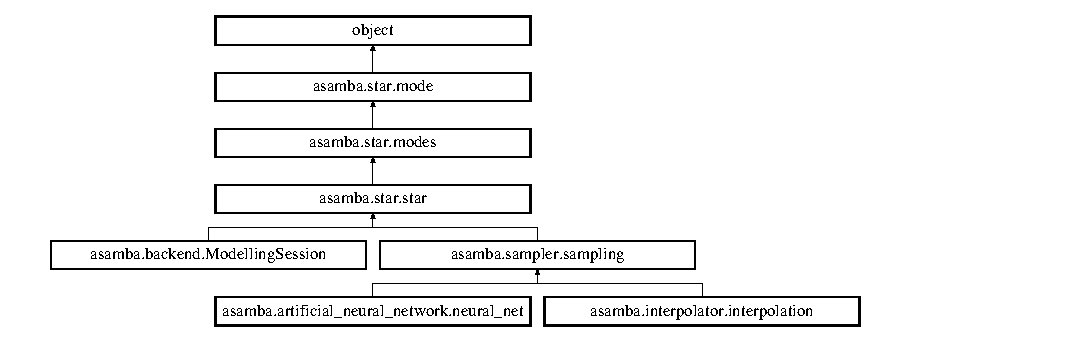
\includegraphics[height=4.148148cm]{classasamba_1_1star_1_1star}
\end{center}
\end{figure}
\subsection*{Public Member Functions}
\begin{DoxyCompactItemize}
\item 
\mbox{\Hypertarget{classasamba_1_1star_1_1star_a5e1bfb2e0171a571b99aeb125afde4a4}\label{classasamba_1_1star_1_1star_a5e1bfb2e0171a571b99aeb125afde4a4}} 
def {\bfseries \+\_\+\+\_\+init\+\_\+\+\_\+} (self)
\item 
def \hyperlink{classasamba_1_1star_1_1star_af0cfdd4049f081617d13919decddc5af}{set} (self, attr, val)
\begin{DoxyCompactList}\small\item\em Setter. \end{DoxyCompactList}\item 
def \hyperlink{classasamba_1_1star_1_1star_a388403867f4905df1f6c983131535379}{get} (self, attr)
\begin{DoxyCompactList}\small\item\em Getter. \end{DoxyCompactList}\item 
def \hyperlink{classasamba_1_1star_1_1star_aec75624cd5c21ff1f0121012ccb01903}{load\+\_\+star\+\_\+from\+\_\+inlist} (self, filename)
\begin{DoxyCompactList}\small\item\em Methods. \end{DoxyCompactList}\end{DoxyCompactItemize}
\subsection*{Public Attributes}
\begin{DoxyCompactItemize}
\item 
\mbox{\Hypertarget{classasamba_1_1star_1_1star_a5745ec51cebce66c39d5ab488a70bb15}\label{classasamba_1_1star_1_1star_a5745ec51cebce66c39d5ab488a70bb15}} 
{\bfseries name}
\item 
\mbox{\Hypertarget{classasamba_1_1star_1_1star_a9d186d20067653c388ccc45744753b53}\label{classasamba_1_1star_1_1star_a9d186d20067653c388ccc45744753b53}} 
{\bfseries other\+\_\+names}
\item 
\mbox{\Hypertarget{classasamba_1_1star_1_1star_ad0bc9c0a55cba0f8afee7731b850e2c9}\label{classasamba_1_1star_1_1star_ad0bc9c0a55cba0f8afee7731b850e2c9}} 
{\bfseries is\+\_\+binary}
\item 
\mbox{\Hypertarget{classasamba_1_1star_1_1star_ad8001e2b6fda7552b31a0aff5b0f729a}\label{classasamba_1_1star_1_1star_ad8001e2b6fda7552b31a0aff5b0f729a}} 
{\bfseries spectral\+\_\+type}
\item 
\mbox{\Hypertarget{classasamba_1_1star_1_1star_ac55e92d39e4e187226b7f1b82fe65904}\label{classasamba_1_1star_1_1star_ac55e92d39e4e187226b7f1b82fe65904}} 
{\bfseries luminosity\+\_\+class}
\item 
\mbox{\Hypertarget{classasamba_1_1star_1_1star_ac10038a76ff2953d48b5820879ec7e68}\label{classasamba_1_1star_1_1star_ac10038a76ff2953d48b5820879ec7e68}} 
{\bfseries is\+\_\+magnetic}
\item 
\mbox{\Hypertarget{classasamba_1_1star_1_1star_a8af04f7854ae81d4b6a63e69f73b6c8c}\label{classasamba_1_1star_1_1star_a8af04f7854ae81d4b6a63e69f73b6c8c}} 
{\bfseries B\+\_\+mag}
\item 
\mbox{\Hypertarget{classasamba_1_1star_1_1star_a1b394ea5457aaaf3c1275eedcb640e9d}\label{classasamba_1_1star_1_1star_a1b394ea5457aaaf3c1275eedcb640e9d}} 
{\bfseries B\+\_\+mag\+\_\+err}
\item 
\mbox{\Hypertarget{classasamba_1_1star_1_1star_a315e6a69358382cf59800a1e20c5d9c2}\label{classasamba_1_1star_1_1star_a315e6a69358382cf59800a1e20c5d9c2}} 
{\bfseries variability\+\_\+type}
\item 
\mbox{\Hypertarget{classasamba_1_1star_1_1star_af2e769fdae7cfa43881fb02c1c382cb6}\label{classasamba_1_1star_1_1star_af2e769fdae7cfa43881fb02c1c382cb6}} 
{\bfseries Teff}
\item 
\mbox{\Hypertarget{classasamba_1_1star_1_1star_a0077d9c97ec3a441c8a145111a49b5c8}\label{classasamba_1_1star_1_1star_a0077d9c97ec3a441c8a145111a49b5c8}} 
{\bfseries Teff\+\_\+err\+\_\+lower}
\item 
\mbox{\Hypertarget{classasamba_1_1star_1_1star_a8724c262f903a1d1d35444d4c6d57565}\label{classasamba_1_1star_1_1star_a8724c262f903a1d1d35444d4c6d57565}} 
{\bfseries Teff\+\_\+err\+\_\+upper}
\item 
\mbox{\Hypertarget{classasamba_1_1star_1_1star_aa4be7611f7395d3d73f357a87bd11571}\label{classasamba_1_1star_1_1star_aa4be7611f7395d3d73f357a87bd11571}} 
{\bfseries log\+\_\+\+Teff}
\item 
\mbox{\Hypertarget{classasamba_1_1star_1_1star_adb749bbdfe31ada03e6ac781afa7f67f}\label{classasamba_1_1star_1_1star_adb749bbdfe31ada03e6ac781afa7f67f}} 
{\bfseries log\+\_\+\+Teff\+\_\+err\+\_\+lower}
\item 
\mbox{\Hypertarget{classasamba_1_1star_1_1star_a7cec1d140d2c0a599fda83079d565e8e}\label{classasamba_1_1star_1_1star_a7cec1d140d2c0a599fda83079d565e8e}} 
{\bfseries log\+\_\+\+Teff\+\_\+err\+\_\+upper}
\item 
\mbox{\Hypertarget{classasamba_1_1star_1_1star_a53aa33233065675a0f180dfba93b8c52}\label{classasamba_1_1star_1_1star_a53aa33233065675a0f180dfba93b8c52}} 
{\bfseries log\+\_\+g}
\item 
\mbox{\Hypertarget{classasamba_1_1star_1_1star_ad78d960a48114d00ecd25ee8c16d2cdb}\label{classasamba_1_1star_1_1star_ad78d960a48114d00ecd25ee8c16d2cdb}} 
{\bfseries log\+\_\+g\+\_\+err\+\_\+lower}
\item 
\mbox{\Hypertarget{classasamba_1_1star_1_1star_a31964770e19faa83dc7c9604cce6d5a1}\label{classasamba_1_1star_1_1star_a31964770e19faa83dc7c9604cce6d5a1}} 
{\bfseries log\+\_\+g\+\_\+err\+\_\+upper}
\item 
\mbox{\Hypertarget{classasamba_1_1star_1_1star_a2505f4e279d9ae79b3569bd278886b6b}\label{classasamba_1_1star_1_1star_a2505f4e279d9ae79b3569bd278886b6b}} 
{\bfseries parallax}
\item 
\mbox{\Hypertarget{classasamba_1_1star_1_1star_a8e9fe42ae1c67d44feadcb46e7f9ee04}\label{classasamba_1_1star_1_1star_a8e9fe42ae1c67d44feadcb46e7f9ee04}} 
{\bfseries parallax\+\_\+err}
\item 
\mbox{\Hypertarget{classasamba_1_1star_1_1star_aad442595239d19de5f4e535a6e4ba719}\label{classasamba_1_1star_1_1star_aad442595239d19de5f4e535a6e4ba719}} 
{\bfseries luminosity}
\item 
\mbox{\Hypertarget{classasamba_1_1star_1_1star_a8c2b98cc5f2898bcbd7ddd1dd5761dec}\label{classasamba_1_1star_1_1star_a8c2b98cc5f2898bcbd7ddd1dd5761dec}} 
{\bfseries luminosity\+\_\+err}
\item 
\mbox{\Hypertarget{classasamba_1_1star_1_1star_a9aa673c778c4adcfff8c421a8ffdc6c8}\label{classasamba_1_1star_1_1star_a9aa673c778c4adcfff8c421a8ffdc6c8}} 
{\bfseries v\+\_\+sini}
\item 
\mbox{\Hypertarget{classasamba_1_1star_1_1star_a7b213f48369e1451f0184cb4697d7c2f}\label{classasamba_1_1star_1_1star_a7b213f48369e1451f0184cb4697d7c2f}} 
{\bfseries v\+\_\+sini\+\_\+err}
\item 
\mbox{\Hypertarget{classasamba_1_1star_1_1star_a9779fa966ac15c207b45e03f21bd8ee6}\label{classasamba_1_1star_1_1star_a9779fa966ac15c207b45e03f21bd8ee6}} 
{\bfseries freq\+\_\+rot}
\item 
\mbox{\Hypertarget{classasamba_1_1star_1_1star_a1a8239990c1e0a2829ed191a6289789f}\label{classasamba_1_1star_1_1star_a1a8239990c1e0a2829ed191a6289789f}} 
{\bfseries freq\+\_\+rot\+\_\+err}
\item 
\mbox{\Hypertarget{classasamba_1_1star_1_1star_a111223a6ccc57b0de6f4a28b55aae5ad}\label{classasamba_1_1star_1_1star_a111223a6ccc57b0de6f4a28b55aae5ad}} 
{\bfseries v\+\_\+micro}
\item 
\mbox{\Hypertarget{classasamba_1_1star_1_1star_ac67dfd88fd1247305764f4ce22c104ec}\label{classasamba_1_1star_1_1star_ac67dfd88fd1247305764f4ce22c104ec}} 
{\bfseries v\+\_\+macro}
\item 
\mbox{\Hypertarget{classasamba_1_1star_1_1star_ae6949e6dff3cb5640f3feda4222bfcb3}\label{classasamba_1_1star_1_1star_ae6949e6dff3cb5640f3feda4222bfcb3}} 
{\bfseries mass}
\item 
\mbox{\Hypertarget{classasamba_1_1star_1_1star_a566db35a0b6fc907c77c8ec7b3d266ff}\label{classasamba_1_1star_1_1star_a566db35a0b6fc907c77c8ec7b3d266ff}} 
{\bfseries mass\+\_\+err}
\item 
\mbox{\Hypertarget{classasamba_1_1star_1_1star_a40ef93f67cc28659517c4426f9e95cd4}\label{classasamba_1_1star_1_1star_a40ef93f67cc28659517c4426f9e95cd4}} 
{\bfseries Z}
\item 
\mbox{\Hypertarget{classasamba_1_1star_1_1star_ab2e35d0a4ebb0c04aee1af74bb75037a}\label{classasamba_1_1star_1_1star_ab2e35d0a4ebb0c04aee1af74bb75037a}} 
{\bfseries Fe\+\_\+H}
\item 
\mbox{\Hypertarget{classasamba_1_1star_1_1star_a6b40508ece199d419ed2f9622de24c76}\label{classasamba_1_1star_1_1star_a6b40508ece199d419ed2f9622de24c76}} 
{\bfseries Z\+\_\+err}
\item 
\mbox{\Hypertarget{classasamba_1_1star_1_1star_afd36b3493c92b62b661eb2804d289274}\label{classasamba_1_1star_1_1star_afd36b3493c92b62b661eb2804d289274}} 
{\bfseries Fe\+\_\+\+H\+\_\+err}
\item 
\mbox{\Hypertarget{classasamba_1_1star_1_1star_ad35253c9cbf322657b2449952467968e}\label{classasamba_1_1star_1_1star_ad35253c9cbf322657b2449952467968e}} 
{\bfseries alpha\+\_\+ov}
\item 
\mbox{\Hypertarget{classasamba_1_1star_1_1star_afa18930c32b371d53fa4e1381b0d0d5d}\label{classasamba_1_1star_1_1star_afa18930c32b371d53fa4e1381b0d0d5d}} 
{\bfseries alpha\+\_\+ov\+\_\+err}
\item 
\mbox{\Hypertarget{classasamba_1_1star_1_1star_a61bd9518c71fccec5bfd50ab81b07d56}\label{classasamba_1_1star_1_1star_a61bd9518c71fccec5bfd50ab81b07d56}} 
{\bfseries f\+\_\+ov}
\item 
\mbox{\Hypertarget{classasamba_1_1star_1_1star_a35bbe1a77c317d3c603ce8ffeb248b74}\label{classasamba_1_1star_1_1star_a35bbe1a77c317d3c603ce8ffeb248b74}} 
{\bfseries f\+\_\+ov\+\_\+err}
\item 
\mbox{\Hypertarget{classasamba_1_1star_1_1star_a7f754d7a4dec982176203eb686f68129}\label{classasamba_1_1star_1_1star_a7f754d7a4dec982176203eb686f68129}} 
{\bfseries surface\+\_\+\+He}
\item 
\mbox{\Hypertarget{classasamba_1_1star_1_1star_ae627cb5b1c43489828a75cafa995fbb1}\label{classasamba_1_1star_1_1star_ae627cb5b1c43489828a75cafa995fbb1}} 
{\bfseries surface\+\_\+\+He\+\_\+err}
\item 
\mbox{\Hypertarget{classasamba_1_1star_1_1star_ac1835a6bfe752d6fa27a6579399b63a9}\label{classasamba_1_1star_1_1star_ac1835a6bfe752d6fa27a6579399b63a9}} 
{\bfseries surface\+\_\+C}
\item 
\mbox{\Hypertarget{classasamba_1_1star_1_1star_ad2f55e87023ba67ad276cd7165aadb48}\label{classasamba_1_1star_1_1star_ad2f55e87023ba67ad276cd7165aadb48}} 
{\bfseries surface\+\_\+\+C\+\_\+err}
\item 
\mbox{\Hypertarget{classasamba_1_1star_1_1star_a89178eb40fe3ef9f6edc649b963c9aad}\label{classasamba_1_1star_1_1star_a89178eb40fe3ef9f6edc649b963c9aad}} 
{\bfseries surface\+\_\+N}
\item 
\mbox{\Hypertarget{classasamba_1_1star_1_1star_a7f4d24c9c4456100f1c25f2c8e485eb6}\label{classasamba_1_1star_1_1star_a7f4d24c9c4456100f1c25f2c8e485eb6}} 
{\bfseries surface\+\_\+\+N\+\_\+err}
\item 
\mbox{\Hypertarget{classasamba_1_1star_1_1star_ac79085a11f7959ceae8abaf5463891e8}\label{classasamba_1_1star_1_1star_ac79085a11f7959ceae8abaf5463891e8}} 
{\bfseries surface\+\_\+O}
\item 
\mbox{\Hypertarget{classasamba_1_1star_1_1star_a505218c62a31e5bb61b2822040d87028}\label{classasamba_1_1star_1_1star_a505218c62a31e5bb61b2822040d87028}} 
{\bfseries surface\+\_\+\+O\+\_\+err}
\item 
\mbox{\Hypertarget{classasamba_1_1star_1_1star_a8252f0a54aa01752eadcb1342a6c35cd}\label{classasamba_1_1star_1_1star_a8252f0a54aa01752eadcb1342a6c35cd}} 
{\bfseries center\+\_\+H}
\item 
\mbox{\Hypertarget{classasamba_1_1star_1_1star_a4c8093e51c1fe37d10c9186aaa972793}\label{classasamba_1_1star_1_1star_a4c8093e51c1fe37d10c9186aaa972793}} 
{\bfseries center\+\_\+\+H\+\_\+err}
\item 
\mbox{\Hypertarget{classasamba_1_1star_1_1star_abc2e548e03a7224e0aed1f5cd69317be}\label{classasamba_1_1star_1_1star_abc2e548e03a7224e0aed1f5cd69317be}} 
{\bfseries center\+\_\+\+He}
\item 
\mbox{\Hypertarget{classasamba_1_1star_1_1star_a7515833b54158162ef38212c9babb910}\label{classasamba_1_1star_1_1star_a7515833b54158162ef38212c9babb910}} 
{\bfseries center\+\_\+\+He\+\_\+err}
\item 
\mbox{\Hypertarget{classasamba_1_1star_1_1star_a89631fb850b002759c4e08b3377536a3}\label{classasamba_1_1star_1_1star_a89631fb850b002759c4e08b3377536a3}} 
{\bfseries principal\+\_\+investigator}
\item 
\mbox{\Hypertarget{classasamba_1_1star_1_1star_a6e1ada4846d84c80523313edaa09b5bc}\label{classasamba_1_1star_1_1star_a6e1ada4846d84c80523313edaa09b5bc}} 
{\bfseries references}
\item 
\mbox{\Hypertarget{classasamba_1_1star_1_1star_a5d06a6f0a74d4934527b5776b6d16a60}\label{classasamba_1_1star_1_1star_a5d06a6f0a74d4934527b5776b6d16a60}} 
{\bfseries url}
\end{DoxyCompactItemize}


\subsection{Detailed Description}
\begin{DoxyVerb}Container for all possible observables of a star, and the uncertainties, if available. This class
inherits the "mode()" class.
\end{DoxyVerb}
 

Definition at line 259 of file star.\+py.



\subsection{Member Function Documentation}
\mbox{\Hypertarget{classasamba_1_1star_1_1star_a388403867f4905df1f6c983131535379}\label{classasamba_1_1star_1_1star_a388403867f4905df1f6c983131535379}} 
\index{asamba\+::star\+::star@{asamba\+::star\+::star}!get@{get}}
\index{get@{get}!asamba\+::star\+::star@{asamba\+::star\+::star}}
\subsubsection{\texorpdfstring{get()}{get()}}
{\footnotesize\ttfamily def asamba.\+star.\+star.\+get (\begin{DoxyParamCaption}\item[{}]{self,  }\item[{}]{attr }\end{DoxyParamCaption})}



Getter. 

\begin{DoxyVerb}Getter \end{DoxyVerb}
 

Definition at line 411 of file star.\+py.

\mbox{\Hypertarget{classasamba_1_1star_1_1star_aec75624cd5c21ff1f0121012ccb01903}\label{classasamba_1_1star_1_1star_aec75624cd5c21ff1f0121012ccb01903}} 
\index{asamba\+::star\+::star@{asamba\+::star\+::star}!load\+\_\+star\+\_\+from\+\_\+inlist@{load\+\_\+star\+\_\+from\+\_\+inlist}}
\index{load\+\_\+star\+\_\+from\+\_\+inlist@{load\+\_\+star\+\_\+from\+\_\+inlist}!asamba\+::star\+::star@{asamba\+::star\+::star}}
\subsubsection{\texorpdfstring{load\+\_\+star\+\_\+from\+\_\+inlist()}{load\_star\_from\_inlist()}}
{\footnotesize\ttfamily def asamba.\+star.\+star.\+load\+\_\+star\+\_\+from\+\_\+inlist (\begin{DoxyParamCaption}\item[{}]{self,  }\item[{}]{filename }\end{DoxyParamCaption})}



Methods. 

\begin{DoxyVerb}One can set the attributes of a specific star all from an inlist. This method is used by the 
backend module, but can be widely used in any script.

@param self: an instance of the star.star() class 
@type self: object
@param filename: full path to the star inlist
@type filename: str
@return: None
\end{DoxyVerb}
 

Definition at line 422 of file star.\+py.

\mbox{\Hypertarget{classasamba_1_1star_1_1star_af0cfdd4049f081617d13919decddc5af}\label{classasamba_1_1star_1_1star_af0cfdd4049f081617d13919decddc5af}} 
\index{asamba\+::star\+::star@{asamba\+::star\+::star}!set@{set}}
\index{set@{set}!asamba\+::star\+::star@{asamba\+::star\+::star}}
\subsubsection{\texorpdfstring{set()}{set()}}
{\footnotesize\ttfamily def asamba.\+star.\+star.\+set (\begin{DoxyParamCaption}\item[{}]{self,  }\item[{}]{attr,  }\item[{}]{val }\end{DoxyParamCaption})}



Setter. 

\begin{DoxyVerb}Setter \end{DoxyVerb}
 

Definition at line 400 of file star.\+py.



The documentation for this class was generated from the following file\+:\begin{DoxyCompactItemize}
\item 
star.\+py\end{DoxyCompactItemize}

\hypertarget{classasamba_1_1var__def_1_1track}{}\section{asamba.\+var\+\_\+def.\+track Class Reference}
\label{classasamba_1_1var__def_1_1track}\index{asamba.\+var\+\_\+def.\+track@{asamba.\+var\+\_\+def.\+track}}


Inheritance diagram for asamba.\+var\+\_\+def.\+track\+:
% FIG 0


Collaboration diagram for asamba.\+var\+\_\+def.\+track\+:
% FIG 1
\subsection*{Public Member Functions}
\begin{DoxyCompactItemize}
\item 
def \hyperlink{classasamba_1_1var__def_1_1track_a4b2441ffcfecbec92fb57d7d57aa3939}{\+\_\+\+\_\+init\+\_\+\+\_\+} (self, M\+\_\+ini=-\/1.\+0, Z=-\/1.\+0, fov=-\/1.\+0, logD=-\/1.\+0)
\item 
\mbox{\Hypertarget{classasamba_1_1var__def_1_1track_aed957132df7a7e728252aad31b93ea67}\label{classasamba_1_1var__def_1_1track_aed957132df7a7e728252aad31b93ea67}} 
def {\bfseries \+\_\+\+\_\+exit\+\_\+\+\_\+} (self, type, value, traceback)
\item 
\mbox{\Hypertarget{classasamba_1_1var__def_1_1track_a5f46732cb3a31e15e2aed17688a403ea}\label{classasamba_1_1var__def_1_1track_a5f46732cb3a31e15e2aed17688a403ea}} 
def {\bfseries set\+\_\+\+M\+\_\+ini} (self, M\+\_\+ini)
\item 
\mbox{\Hypertarget{classasamba_1_1var__def_1_1track_ad70395a3e579d489e6234232629e341f}\label{classasamba_1_1var__def_1_1track_ad70395a3e579d489e6234232629e341f}} 
def {\bfseries set\+\_\+Z} (self, Z)
\item 
\mbox{\Hypertarget{classasamba_1_1var__def_1_1track_a26354c8dfd8dc3ee2cc1557ad1ab299d}\label{classasamba_1_1var__def_1_1track_a26354c8dfd8dc3ee2cc1557ad1ab299d}} 
def {\bfseries set\+\_\+fov} (self, fov)
\item 
\mbox{\Hypertarget{classasamba_1_1var__def_1_1track_a62f1ee4781b07e529f159ad292f199a9}\label{classasamba_1_1var__def_1_1track_a62f1ee4781b07e529f159ad292f199a9}} 
def {\bfseries set\+\_\+logD} (self, logD)
\item 
\mbox{\Hypertarget{classasamba_1_1var__def_1_1track_aac1969da3c80cef07dac95d9d19a5267}\label{classasamba_1_1var__def_1_1track_aac1969da3c80cef07dac95d9d19a5267}} 
def {\bfseries set\+\_\+filename} (self, filename)
\item 
\mbox{\Hypertarget{classasamba_1_1var__def_1_1track_ac30f57980f1f11f3d986e3dcb654d0c3}\label{classasamba_1_1var__def_1_1track_ac30f57980f1f11f3d986e3dcb654d0c3}} 
def {\bfseries get\+\_\+\+M\+\_\+ini} (self)
\item 
\mbox{\Hypertarget{classasamba_1_1var__def_1_1track_a18150ada4b8ce715f9bbb56434fdf83e}\label{classasamba_1_1var__def_1_1track_a18150ada4b8ce715f9bbb56434fdf83e}} 
def {\bfseries get\+\_\+Z} (self)
\item 
\mbox{\Hypertarget{classasamba_1_1var__def_1_1track_a15bd996fa8ef66ac4575a35ace31a0af}\label{classasamba_1_1var__def_1_1track_a15bd996fa8ef66ac4575a35ace31a0af}} 
def {\bfseries get\+\_\+fov} (self)
\item 
\mbox{\Hypertarget{classasamba_1_1var__def_1_1track_ac9944e9e2c420b290800b89499a1b46e}\label{classasamba_1_1var__def_1_1track_ac9944e9e2c420b290800b89499a1b46e}} 
def {\bfseries get\+\_\+logD} (self)
\item 
\mbox{\Hypertarget{classasamba_1_1var__def_1_1track_a481ec6ec42ef88569f7f7460e71a4301}\label{classasamba_1_1var__def_1_1track_a481ec6ec42ef88569f7f7460e71a4301}} 
def {\bfseries get\+\_\+filename} (self)
\item 
def \hyperlink{classasamba_1_1var__def_1_1track_aec000211bbf1940b5c05b0bcd380fc2a}{get\+\_\+attr\+\_\+as\+\_\+dic} (self)
\end{DoxyCompactItemize}
\subsection*{Public Attributes}
\begin{DoxyCompactItemize}
\item 
\mbox{\Hypertarget{classasamba_1_1var__def_1_1track_aa3dbc15bdcf66b74d94c7eec646d1130}\label{classasamba_1_1var__def_1_1track_aa3dbc15bdcf66b74d94c7eec646d1130}} 
{\bfseries M\+\_\+ini}
\item 
\mbox{\Hypertarget{classasamba_1_1var__def_1_1track_a2c417501a83649d928d086a3145ab209}\label{classasamba_1_1var__def_1_1track_a2c417501a83649d928d086a3145ab209}} 
{\bfseries Z}
\item 
\mbox{\Hypertarget{classasamba_1_1var__def_1_1track_a0f34b50e996c9be9d9f0832a25ab33cb}\label{classasamba_1_1var__def_1_1track_a0f34b50e996c9be9d9f0832a25ab33cb}} 
{\bfseries fov}
\item 
\mbox{\Hypertarget{classasamba_1_1var__def_1_1track_a76991863706f1d8838b4864957d50ddd}\label{classasamba_1_1var__def_1_1track_a76991863706f1d8838b4864957d50ddd}} 
{\bfseries logD}
\item 
\mbox{\Hypertarget{classasamba_1_1var__def_1_1track_af8f0ad459781b31152e8a2329a788886}\label{classasamba_1_1var__def_1_1track_af8f0ad459781b31152e8a2329a788886}} 
{\bfseries filename}
\end{DoxyCompactItemize}


\subsection{Detailed Description}
\begin{DoxyVerb}Class object that stores the data for MESA tracks
\end{DoxyVerb}
 

Definition at line 18 of file var\+\_\+def.\+py.



\subsection{Constructor \& Destructor Documentation}
\mbox{\Hypertarget{classasamba_1_1var__def_1_1track_a4b2441ffcfecbec92fb57d7d57aa3939}\label{classasamba_1_1var__def_1_1track_a4b2441ffcfecbec92fb57d7d57aa3939}} 
\index{asamba\+::var\+\_\+def\+::track@{asamba\+::var\+\_\+def\+::track}!\+\_\+\+\_\+init\+\_\+\+\_\+@{\+\_\+\+\_\+init\+\_\+\+\_\+}}
\index{\+\_\+\+\_\+init\+\_\+\+\_\+@{\+\_\+\+\_\+init\+\_\+\+\_\+}!asamba\+::var\+\_\+def\+::track@{asamba\+::var\+\_\+def\+::track}}
\subsubsection{\texorpdfstring{\+\_\+\+\_\+init\+\_\+\+\_\+()}{\_\_init\_\_()}}
{\footnotesize\ttfamily def asamba.\+var\+\_\+def.\+track.\+\_\+\+\_\+init\+\_\+\+\_\+ (\begin{DoxyParamCaption}\item[{}]{self,  }\item[{}]{M\+\_\+ini = {\ttfamily -\/1.0},  }\item[{}]{Z = {\ttfamily -\/1.0},  }\item[{}]{fov = {\ttfamily -\/1.0},  }\item[{}]{logD = {\ttfamily -\/1.0} }\end{DoxyParamCaption})}

\begin{DoxyVerb}Constructor that stores the mass, metalicity, overshoot and extra diffusive mixing per each 
track. By default, the attributes are set to "-1.0" as a physically meaningless initial value,
to facilitate more convenient capturing of wrong initializations. E.g. you can initialize a track
as:

>>>a_track = var_def.track(M_ini=12.0, Z=0.014, fov=0.024, logD=2.25)

@param M_ini: the initial mass in solar unit
@type M_ini: float
@param Z: metallicity (where the solar metallicity from Asplund et al. 2009 is 0.014)
@type Z: float
@param fov: the exponential overshoot free parameter (see e.g. Eq. 2 in Moravveji et al.
   2016, ApJ)
@type fov: float
@param logD: the (logarithm of the) constant diffusive mixing in the radiative envelope.
   See e.g. Fig. 2a in Moravveji et al. (2016, ApJ)
@type logD: float
\end{DoxyVerb}
 

Definition at line 22 of file var\+\_\+def.\+py.



\subsection{Member Function Documentation}
\mbox{\Hypertarget{classasamba_1_1var__def_1_1track_aec000211bbf1940b5c05b0bcd380fc2a}\label{classasamba_1_1var__def_1_1track_aec000211bbf1940b5c05b0bcd380fc2a}} 
\index{asamba\+::var\+\_\+def\+::track@{asamba\+::var\+\_\+def\+::track}!get\+\_\+attr\+\_\+as\+\_\+dic@{get\+\_\+attr\+\_\+as\+\_\+dic}}
\index{get\+\_\+attr\+\_\+as\+\_\+dic@{get\+\_\+attr\+\_\+as\+\_\+dic}!asamba\+::var\+\_\+def\+::track@{asamba\+::var\+\_\+def\+::track}}
\subsubsection{\texorpdfstring{get\+\_\+attr\+\_\+as\+\_\+dic()}{get\_attr\_as\_dic()}}
{\footnotesize\ttfamily def asamba.\+var\+\_\+def.\+track.\+get\+\_\+attr\+\_\+as\+\_\+dic (\begin{DoxyParamCaption}\item[{}]{self }\end{DoxyParamCaption})}

\begin{DoxyVerb}Convert the attributes of the "track" object into a dictionary, with the attribute names as keys
\end{DoxyVerb}
 

Definition at line 94 of file var\+\_\+def.\+py.



The documentation for this class was generated from the following file\+:\begin{DoxyCompactItemize}
\item 
var\+\_\+def.\+py\end{DoxyCompactItemize}

\hypertarget{classasamba_1_1var__def_1_1tracks}{}\section{asamba.\+var\+\_\+def.\+tracks Class Reference}
\label{classasamba_1_1var__def_1_1tracks}\index{asamba.\+var\+\_\+def.\+tracks@{asamba.\+var\+\_\+def.\+tracks}}


Inheritance diagram for asamba.\+var\+\_\+def.\+tracks\+:
% FIG 0


Collaboration diagram for asamba.\+var\+\_\+def.\+tracks\+:
% FIG 1
\subsection*{Public Member Functions}
\begin{DoxyCompactItemize}
\item 
def \hyperlink{classasamba_1_1var__def_1_1tracks_a317ae0c8a333fcbcf9e907f9f09d4c48}{\+\_\+\+\_\+init\+\_\+\+\_\+} (self, dir\+\_\+repos)
\item 
\mbox{\Hypertarget{classasamba_1_1var__def_1_1tracks_a3fa0854d4982624b4a2f954c745e9f6d}\label{classasamba_1_1var__def_1_1tracks_a3fa0854d4982624b4a2f954c745e9f6d}} 
def {\bfseries \+\_\+\+\_\+enter\+\_\+\+\_\+} (self)
\item 
\mbox{\Hypertarget{classasamba_1_1var__def_1_1tracks_a2f766da66983a7e055916b8a2c6d8c8b}\label{classasamba_1_1var__def_1_1tracks_a2f766da66983a7e055916b8a2c6d8c8b}} 
def {\bfseries \+\_\+\+\_\+exit\+\_\+\+\_\+} (self, type, value, traceback)
\item 
\mbox{\Hypertarget{classasamba_1_1var__def_1_1tracks_acbfad91a58aad6c1d94d4697c5da07f2}\label{classasamba_1_1var__def_1_1tracks_acbfad91a58aad6c1d94d4697c5da07f2}} 
def {\bfseries set\+\_\+dir\+\_\+repos} (self, dir\+\_\+repos)
\item 
\mbox{\Hypertarget{classasamba_1_1var__def_1_1tracks_a3a604a91219aee4ceefe39ec53a11909}\label{classasamba_1_1var__def_1_1tracks_a3a604a91219aee4ceefe39ec53a11909}} 
def {\bfseries set\+\_\+mass\+\_\+search\+\_\+pattern} (self, mass\+\_\+search\+\_\+pattern)
\item 
\mbox{\Hypertarget{classasamba_1_1var__def_1_1tracks_ade5767a5bf3585e28b799c9f0293cc47}\label{classasamba_1_1var__def_1_1tracks_ade5767a5bf3585e28b799c9f0293cc47}} 
def {\bfseries set\+\_\+hist\+\_\+search\+\_\+pattern} (self, hist\+\_\+search\+\_\+pattern)
\item 
\mbox{\Hypertarget{classasamba_1_1var__def_1_1tracks_a9915164166bfc2053982747a020ba9e7}\label{classasamba_1_1var__def_1_1tracks_a9915164166bfc2053982747a020ba9e7}} 
def {\bfseries set\+\_\+hist\+\_\+extension} (self, hist\+\_\+extension)
\item 
\mbox{\Hypertarget{classasamba_1_1var__def_1_1tracks_aaa05dae334bf401bb6a5a68c3bdd44aa}\label{classasamba_1_1var__def_1_1tracks_aaa05dae334bf401bb6a5a68c3bdd44aa}} 
def {\bfseries set\+\_\+n\+\_\+dirs\+\_\+\+M\+\_\+ini} (self, n\+\_\+dirs\+\_\+\+M\+\_\+ini)
\item 
\mbox{\Hypertarget{classasamba_1_1var__def_1_1tracks_ab4111e6b26edf9e76ceb96bec4763064}\label{classasamba_1_1var__def_1_1tracks_ab4111e6b26edf9e76ceb96bec4763064}} 
def {\bfseries set\+\_\+list\+\_\+dirs\+\_\+\+M\+\_\+ini} (self, list\+\_\+dirs\+\_\+\+M\+\_\+ini)
\item 
\mbox{\Hypertarget{classasamba_1_1var__def_1_1tracks_a148ce756693d708911775b3c2820c1f0}\label{classasamba_1_1var__def_1_1tracks_a148ce756693d708911775b3c2820c1f0}} 
def {\bfseries set\+\_\+n\+\_\+tracks} (self, n\+\_\+tracks)
\item 
\mbox{\Hypertarget{classasamba_1_1var__def_1_1tracks_ad8905211d69ef4b3199cedc83bc94803}\label{classasamba_1_1var__def_1_1tracks_ad8905211d69ef4b3199cedc83bc94803}} 
def {\bfseries set\+\_\+list\+\_\+tracks} (self, list\+\_\+tracks)
\item 
def \hyperlink{classasamba_1_1var__def_1_1tracks_abd062bf94f2cd69eab54d2a081bebad1}{set\+\_\+mass\+\_\+directories} (self)
\item 
def \hyperlink{classasamba_1_1var__def_1_1tracks_a743c0e7e4af42a5c67f8a4be54a7d3c6}{set\+\_\+track\+\_\+parameters} (self)
\item 
\mbox{\Hypertarget{classasamba_1_1var__def_1_1tracks_a8a24194336cd06e10cd0e4431cff963f}\label{classasamba_1_1var__def_1_1tracks_a8a24194336cd06e10cd0e4431cff963f}} 
def {\bfseries get\+\_\+dir\+\_\+repos} (self)
\item 
\mbox{\Hypertarget{classasamba_1_1var__def_1_1tracks_ae2293a407b4f731e3f76de188de57ec5}\label{classasamba_1_1var__def_1_1tracks_ae2293a407b4f731e3f76de188de57ec5}} 
def {\bfseries get\+\_\+mass\+\_\+search\+\_\+pattern} (self)
\item 
\mbox{\Hypertarget{classasamba_1_1var__def_1_1tracks_aeb2f2c3e19db68028deb8bcd65eee114}\label{classasamba_1_1var__def_1_1tracks_aeb2f2c3e19db68028deb8bcd65eee114}} 
def {\bfseries get\+\_\+hist\+\_\+search\+\_\+pattern} (self)
\item 
\mbox{\Hypertarget{classasamba_1_1var__def_1_1tracks_aac18c3f27f1fe9d5fc9005461f57d000}\label{classasamba_1_1var__def_1_1tracks_aac18c3f27f1fe9d5fc9005461f57d000}} 
def {\bfseries get\+\_\+hist\+\_\+extension} (self)
\item 
\mbox{\Hypertarget{classasamba_1_1var__def_1_1tracks_afab2403696c70d59afc162276a793783}\label{classasamba_1_1var__def_1_1tracks_afab2403696c70d59afc162276a793783}} 
def {\bfseries get\+\_\+n\+\_\+dirs\+\_\+\+M\+\_\+ini} (self)
\item 
\mbox{\Hypertarget{classasamba_1_1var__def_1_1tracks_a25425bb3a9c187e4fb4cfcfc45f794f9}\label{classasamba_1_1var__def_1_1tracks_a25425bb3a9c187e4fb4cfcfc45f794f9}} 
def {\bfseries get\+\_\+list\+\_\+dirs\+\_\+\+M\+\_\+ini} (self)
\item 
\mbox{\Hypertarget{classasamba_1_1var__def_1_1tracks_a180bebc4deeb360ba14d70010103ab9a}\label{classasamba_1_1var__def_1_1tracks_a180bebc4deeb360ba14d70010103ab9a}} 
def {\bfseries get\+\_\+n\+\_\+tracks} (self)
\item 
\mbox{\Hypertarget{classasamba_1_1var__def_1_1tracks_ae8321984c301c8df018c02385c7ceb40}\label{classasamba_1_1var__def_1_1tracks_ae8321984c301c8df018c02385c7ceb40}} 
def {\bfseries get\+\_\+list\+\_\+tracks} (self)
\end{DoxyCompactItemize}
\subsection*{Public Attributes}
\begin{DoxyCompactItemize}
\item 
\mbox{\Hypertarget{classasamba_1_1var__def_1_1tracks_abb5a3f5f51f42ffa33d17cfa59afdf49}\label{classasamba_1_1var__def_1_1tracks_abb5a3f5f51f42ffa33d17cfa59afdf49}} 
{\bfseries dir\+\_\+repos}
\item 
\mbox{\Hypertarget{classasamba_1_1var__def_1_1tracks_a05e8ca115e34ba8146953d8b5ad95ed2}\label{classasamba_1_1var__def_1_1tracks_a05e8ca115e34ba8146953d8b5ad95ed2}} 
{\bfseries mass\+\_\+search\+\_\+pattern}
\item 
\mbox{\Hypertarget{classasamba_1_1var__def_1_1tracks_a714538f69e4e307a4c6fc6608da928a0}\label{classasamba_1_1var__def_1_1tracks_a714538f69e4e307a4c6fc6608da928a0}} 
{\bfseries hist\+\_\+search\+\_\+pattern}
\item 
\mbox{\Hypertarget{classasamba_1_1var__def_1_1tracks_aa594311bba704adf5f31e33c8edc3537}\label{classasamba_1_1var__def_1_1tracks_aa594311bba704adf5f31e33c8edc3537}} 
{\bfseries hist\+\_\+extension}
\item 
\mbox{\Hypertarget{classasamba_1_1var__def_1_1tracks_ad360b83822ae08c5061886f32846ebf0}\label{classasamba_1_1var__def_1_1tracks_ad360b83822ae08c5061886f32846ebf0}} 
{\bfseries n\+\_\+dirs\+\_\+\+M\+\_\+ini}
\item 
\mbox{\Hypertarget{classasamba_1_1var__def_1_1tracks_a5eec02ca2b36e289fc3502ec9fd3995f}\label{classasamba_1_1var__def_1_1tracks_a5eec02ca2b36e289fc3502ec9fd3995f}} 
{\bfseries list\+\_\+dirs\+\_\+\+M\+\_\+ini}
\item 
\mbox{\Hypertarget{classasamba_1_1var__def_1_1tracks_afda95e1c2639e216c0e72ef57324acb4}\label{classasamba_1_1var__def_1_1tracks_afda95e1c2639e216c0e72ef57324acb4}} 
{\bfseries n\+\_\+tracks}
\item 
\mbox{\Hypertarget{classasamba_1_1var__def_1_1tracks_a94088762399d82745bd830791518c155}\label{classasamba_1_1var__def_1_1tracks_a94088762399d82745bd830791518c155}} 
{\bfseries list\+\_\+tracks}
\end{DoxyCompactItemize}


\subsection{Detailed Description}
\begin{DoxyVerb}Class object that agglemerates multiple instances of the "track" object
\end{DoxyVerb}
 

Definition at line 105 of file var\+\_\+def.\+py.



\subsection{Constructor \& Destructor Documentation}
\mbox{\Hypertarget{classasamba_1_1var__def_1_1tracks_a317ae0c8a333fcbcf9e907f9f09d4c48}\label{classasamba_1_1var__def_1_1tracks_a317ae0c8a333fcbcf9e907f9f09d4c48}} 
\index{asamba\+::var\+\_\+def\+::tracks@{asamba\+::var\+\_\+def\+::tracks}!\+\_\+\+\_\+init\+\_\+\+\_\+@{\+\_\+\+\_\+init\+\_\+\+\_\+}}
\index{\+\_\+\+\_\+init\+\_\+\+\_\+@{\+\_\+\+\_\+init\+\_\+\+\_\+}!asamba\+::var\+\_\+def\+::tracks@{asamba\+::var\+\_\+def\+::tracks}}
\subsubsection{\texorpdfstring{\+\_\+\+\_\+init\+\_\+\+\_\+()}{\_\_init\_\_()}}
{\footnotesize\ttfamily def asamba.\+var\+\_\+def.\+tracks.\+\_\+\+\_\+init\+\_\+\+\_\+ (\begin{DoxyParamCaption}\item[{}]{self,  }\item[{}]{dir\+\_\+repos }\end{DoxyParamCaption})}

\begin{DoxyVerb}The constructor of the class. E.g.

>>>some_tracks = var_def.tracks(dir_repos='/home/username/projects/mygrid')

@param dir_repos: Full path to the directory where the grid is stored, e.g. 
   /home/user/projects/asamba-grid
@type dir_repos: string
\end{DoxyVerb}
 

Definition at line 109 of file var\+\_\+def.\+py.



\subsection{Member Function Documentation}
\mbox{\Hypertarget{classasamba_1_1var__def_1_1tracks_abd062bf94f2cd69eab54d2a081bebad1}\label{classasamba_1_1var__def_1_1tracks_abd062bf94f2cd69eab54d2a081bebad1}} 
\index{asamba\+::var\+\_\+def\+::tracks@{asamba\+::var\+\_\+def\+::tracks}!set\+\_\+mass\+\_\+directories@{set\+\_\+mass\+\_\+directories}}
\index{set\+\_\+mass\+\_\+directories@{set\+\_\+mass\+\_\+directories}!asamba\+::var\+\_\+def\+::tracks@{asamba\+::var\+\_\+def\+::tracks}}
\subsubsection{\texorpdfstring{set\+\_\+mass\+\_\+directories()}{set\_mass\_directories()}}
{\footnotesize\ttfamily def asamba.\+var\+\_\+def.\+tracks.\+set\+\_\+mass\+\_\+directories (\begin{DoxyParamCaption}\item[{}]{self }\end{DoxyParamCaption})}

\begin{DoxyVerb}Return the list of directories labelled with track initial masses residing in the repository path.
E.g. the directories have names like "dir_repos/M01.234", "dir_repos/M56.789", and so on.
@result: list of full paths to the mass directories
@rtype: list of strings
\end{DoxyVerb}
 

Definition at line 176 of file var\+\_\+def.\+py.

Here is the call graph for this function\+:
% FIG 2
\mbox{\Hypertarget{classasamba_1_1var__def_1_1tracks_a743c0e7e4af42a5c67f8a4be54a7d3c6}\label{classasamba_1_1var__def_1_1tracks_a743c0e7e4af42a5c67f8a4be54a7d3c6}} 
\index{asamba\+::var\+\_\+def\+::tracks@{asamba\+::var\+\_\+def\+::tracks}!set\+\_\+track\+\_\+parameters@{set\+\_\+track\+\_\+parameters}}
\index{set\+\_\+track\+\_\+parameters@{set\+\_\+track\+\_\+parameters}!asamba\+::var\+\_\+def\+::tracks@{asamba\+::var\+\_\+def\+::tracks}}
\subsubsection{\texorpdfstring{set\+\_\+track\+\_\+parameters()}{set\_track\_parameters()}}
{\footnotesize\ttfamily def asamba.\+var\+\_\+def.\+tracks.\+set\+\_\+track\+\_\+parameters (\begin{DoxyParamCaption}\item[{}]{self }\end{DoxyParamCaption})}

\begin{DoxyVerb}Glob and find all available tracks that are organized inside the repository (hence dir_repos).
The tracks are organized based on their initial mass, and lie inside the "hist" subdirectory, e.g.
"dir_repos/M12.345/hist/M12.345-ov0.010-Z0.018-logD01.23.hist"
Then, the whole track parameters will be stored into the "tracks" object

@param self: an instance of the var_def.tracks() object
@type self: class object
\end{DoxyVerb}
 

Definition at line 201 of file var\+\_\+def.\+py.

Here is the call graph for this function\+:
% FIG 3


The documentation for this class was generated from the following file\+:\begin{DoxyCompactItemize}
\item 
var\+\_\+def.\+py\end{DoxyCompactItemize}

%--- End generated contents ---

% Index
\backmatter
\newpage
\phantomsection
\clearemptydoublepage
\addcontentsline{toc}{chapter}{Index}
\printindex

\end{document}
